\documentclass{cernatlasnote}
\usepackage[colorinlistoftodos]{todonotes}
\usepackage{placeins}
\usepackage{multicol}
\usepackage{tikz}
\usepackage{indentfirst}
% \usepackage{biblatex}
\usetikzlibrary{calc}
\newcommand{\tl}{\ensuremath{\textless}}
\newcommand{\tg}{\ensuremath{\textgreater}}
\newcommand{\mumu}{\ensuremath{\mu^{+}\mu^{-}}}
\newcommand{\ee}{\ensuremath{\e^{+}e^{-}}}
\newcommand{\MGaMC}{\textsc{MG5}\_a\textsc{MC}\xspace}
\newcommand{\GENEVA}{\textsc{geneva}\xspace}
\newcommand{\source}[1]{\caption*{Source: {#1}} }
\newcommand{\Lagr}{\mathcal{L}}
\newcommand{\ppbar}{p$\bar{\text{p}}$\xspace}
\newcommand{\qqbar}{q$\bar{\text{q}}$\xspace}
\newcommand{\bbbar}{b$\bar{\text{b}}$\xspace}
\newcommand{\qtoqg}{q $\rightarrow\text{qg}$\xspace}
\newcommand{\gtogg}{g $\rightarrow\text{gg}$\xspace}
\newcommand{\ttbar}{t$\bar{\text{t}}$\xspace}
\newcommand{\ttbarnospace}{t$\bar{\text{t}}$}
\newcommand{\gtoqqbar}{g $\rightarrow\text{q}\bar{\text{q}}$\xspace}
\newcommand{\gtobbbar}{g $\rightarrow\text{b}\bar{\text{b}}$\xspace}
\newcommand{\met}{\ensuremath{E_{\mathrm{T}}^{\rm miss}} \xspace}
\newcommand{\ptmiss}{\ensuremath{p_{\mathrm{T}}^{\rm miss}}\xspace}
\newcommand{\ptvecmiss}{\ensuremath{\vec{p_{\mathrm{T}}^{\rm miss}}}\xspace}
\newcommand{\deta}{\Delta\eta_{jj}}
\newcommand{\mt}{m_{T}(\tau, \met)}

%\newcommand{\pt}{p_{\text T}\xspace}
\newcommand{\pt}{$p_{\text T}$\xspace}
\newcommand{\ptsq}{$p_{\text T}^{2}$\xspace}
%\newcommand{\pt}{\ensuremath{p_{\mathrm T}\xspace}}
\newcommand{\et}{E$_{\rm T}$\xspace}
\newcommand{\kt}{$k_{\text T}$\xspace}
\newcommand{\ptnospace}{$p_{\rm T}$}
\newcommand{\PYTHIA}{\textsc{pythia}\xspace}
\newcommand{\pythia}{\textsc{pythia}\xspace}
\newcommand{\pythiasix}{\textsc{pythia6}\xspace}
\newcommand{\pythiaeight}{\textsc{pythia8}\xspace}
\newcommand{\pythiaeightp}{\textsc{pythia8.2}\xspace}
\newcommand{\MG}{\textsc{madgraph}\xspace}
\newcommand{\MGfive}{\textsc{madgraph5}\xspace}
\newcommand{\powheg}{\textsc{powheg}\xspace}
\newcommand{\POWHEG}{\textsc{powheg}\xspace}
\newcommand{\powhegbox}{\textsc{powhegbox}\xspace}
\newcommand{\herwig}{\textsc{herwig}\xspace}
\newcommand{\sherpa}{\textsc{sherpa}\xspace}
\newcommand{\SHERPA}{\textsc{sherpa}\xspace}
\newcommand{\GEANT}{\textsc{geant4}\xspace}
%\newcommand{TOPpp}{TOP$^{++}$\xspace}
\newcommand{\qqbarZll}{q$\bar{\text{q}}$ $\rightarrow$ Z $\rightarrow l^{+}l^{-}$}
\newcommand{\MGfiveamc} {\textsc{mg5}\_a\textsc{mc}\xspace}
\newcommand{\MGvATNLO}{\textsc{mg5}\_a\textsc{mc@nlo}\xspace}
\newcommand{\MGfiveatNLO}{\textsc{madgraph5}\_a\textsc{mc@nlo}\xspace}
\newcommand{\ATNLO}{a\textsc{mc@nlo}\xspace}
\newcommand{\MCNLO}{\textsc{mc@nlo}\xspace}
\newcommand{\FEWZ}{\textsc{FEWZ}\xspace}
\newcommand{\Irel}{I$_{\rm rel}$\xspace}
\newcommand{\pTPU}{\ensuremath{p_{\mathrm{T}}^{\mathrm{PU}}}\xspace}
%\usepackage[italic]{hepnames}
\usepackage{hepnames}
\newcommand{\PQb}{b\xspace}
\newcommand{\PQc}{c\xspace}
%\newcommand{\PZ}{Z\xspace}
\newcommand{\cPqb}{b\xspace}
\newcommand{\cPqc}{c\xspace}
\newcommand{\fbinv}{\! fb$^{-1}$\xspace}
\newcommand{\Pell}{ll\xspace}
\newcommand{\TeV}{\,TeV\xspace}
\newcommand{\GeV}{\,GeV\xspace}
\newcommand{\MeV}{\,MeV\xspace}
\newcommand{\cm}{\,cm\xspace}
\newcommand{\m}{\,m\xspace}
\newcommand{\mm}{\,mm\xspace}
\newcommand{\fm}{\,fm\xspace}
\newcommand{\pb}{\,pb\xspace}
\newcommand{\ps}{\,ps\xspace}
\newcommand{\s}{\,s\xspace}
\newcommand{\alpSnospace}{$\alpha_{\rm s}$}
\newcommand{\alpS}{$\alpha_{\rm s}$\xspace}
\newcommand{\cPqt}{t}
\newcommand{\gt}{$>$}
\newcommand{\lt}{$<$}
\newcommand{\gte}{$\geq$}
\newcommand{\lte}{$\leq$}
%\newcommand{\PW}{W}
\newcommand{\DeepCSV}{D\textsc{eep}CSV\xspace}
\newcommand{\diele}{ee\xspace}
\newcommand{\dimu}{$\mu\mu$\xspace}


\title{\centering
Search for a long-lived massive particle decaying into a top quark and light quarks in proton-proton collisions at $\sqrt{s} = 13$ and $13.6$ TeV
}
\author{CMS collaboration}
\date{\today}

% Here is the information that will be entered in the title page
\DocAuthors{A.Paul Vaucelle }
\DocCheckedBy{ D.~Person \\ E.~Person}
\DocApprovedBy{F.~Person \\ G.~Person }
\EDMSDocNo{EXO-24-ZZZZ}
\EDMSDocId{123456}
\draftversion{0.1}

\begin{document}
\maketitle

\begin{abstract}

A search for the associated production of a \mumu pair and a pair of massive long-lived particles (LLP), each decaying into a top quark and two light quarks is presented. The data correspond to an integrated luminosity of 300\fbinv recorded in proton-proton collisions at $\sqrt{s} = 13$ and $13.6$ TeV at the LHC. Machine learning technique is used to distinguish displaced charged particles tracks from the LLP and from the Standard Model background. A study is performed relying on reconstructed displaced vertices. Results are interpreted within the R-parity violated Minimal SuperSymmetric model. 
\end{abstract}

% Make the review table at the bottom of the title page
\vfill
\makereviewtable
\clearpage

% Short documentes dont always need a Table of Content / Figures / Tables, so comment out what is not needed
% \begingroup
% \color{black}
% \tableofcontents
% \pagebreak
% \listoffigures
% \pagebreak
% \listoftables
% \endgroup
% \pagebreak

%%%%%%%%%%%%%%%%%%%%%%%%%%%%%%%%%%%%%%%%%%%%%%%%%%%%%%%%%%%%%%%
%%%%%%%%%%%%%%%%%%%%%%%%%%%%%%%%%%%%%%%%%%%%%%%%%%%%%%%%%%%%%%%
%------------------- SECTION ----------------------------------
%%%%%%%%%%%%%%%%%%%%%%%%%%%%%%%%%%%%%%%%%%%%%%%%%%%%%%%%%%%%%%%
%%%%%%%%%%%%%%%%%%%%%%%%%%%%%%%%%%%%%%%%%%%%%%%%%%%%%%%%%%%%%%%

\section{Introduction}
\label{SEC: INTRO}
The search for long-lived particles (LLP) is highly motivated by many extensions of the Standard Model (SM), as R-Parity Violated Minimal SuperSymmetry Model (RPV-MSSM)~\cite{RPV1, RPV2, RPV3, RPV4}, Split-SUSY~\cite{SPLITSUSY, SPLITSUSY2, SPLITSUSY3, SPLITSUSY4, SPLITSUSY5, SPLITSUSY6}, weakly interacting massive particles~\cite{WIMP1,WIMP2,WIMP3}, Gauge Mediated supersymmetry breaking (GMSB)~\cite{GMSB1,GMSB2, GMSB3}, hidden sector \cite{HS1, HS2, HS3}. However the LLP production cross section can be small in case of a high mass or due to its weak coupling, and dedicated techniques have to be applied to reduce the large SM background.

 Searches for displaced jets and vertices at $\sqrt{13}$ TeV have been reported by ATLAS \cite{ATLAS-CONF-2018-003} \cite{DISJETSATLAS} and CMS \cite{DISJETSCMS} in an inclusive approach, where the displaced vertices are mainly searched in the pixel detectors due to the tracking efficiency decreasing rapidly. 

The peculiar process considered in this paper is characterized by the production of a $Z/\gamma^*$ boson from proton-proton (pp) collisions at the LHC. Then the virtual boson couples to a pair of sleptons, where the considered slepton is here a smuon, assumed to be the next-to-lightest supersymmetric particle (NLSP) and to be short-lived. Since the smuon is the NLSP, it decays into a muon and the Lightest-SuperSymmetric-Particle (LSP) which is the neutralino $\chi^{1}_{0}$. The neutralino can only be bino-like, allowing its decay into a top quark and a virtual stop quark. The stop quark couples to SM quarks via $\lambda^{''}_{312}$ RPV coupling giving a down and a strange quark.
In order to reduce the complexity of the model, no mixing between particles of different generations is considered in the mixing matrices of sleptons and squarks, and left-handed and right-handed mass states are set in equal proportion, but results can be reinterpreted in terms of pure left-handed or right-handed states.

A drawing of the considered signal is depicted in Fig.\ref{fig:Feyn}.
The final state consists of an energetic \mumu pair which can be used to trigger the event, and many jets from the two neutralino decays. If the decays occur in the tracker acceptance, secondary vertices with many tracks can be reconstructed, allowing a significant reduction of the SM backgrounds.

\begin{figure}[ht]
\centering
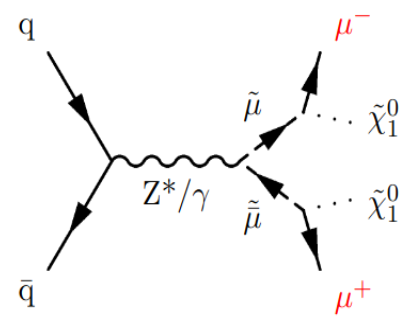
\includegraphics[height=6cm, width=8cm, trim= 0cm 0cm 0cm 0.cm,clip]{images/Feynmann/smuprod.png}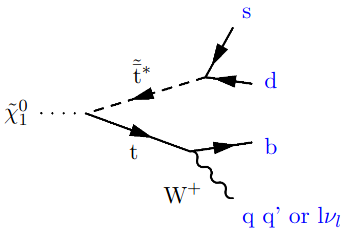
\includegraphics[height=6cm, width=8cm, trim= 0cm 0cm 0cm 0.cm,clip]{images/Feynmann/ChiDecay.png}
\caption{\label{fig:Feyn} Smuon pair production and decay channels.}
\end{figure}

Data recorded in pp collisions at the LHC at center-of-mass energies of 13~TeV from 2016 to 2018 and 13.6~TeV from 2022 to 2024, corresponding to an integrated luminosity of \textcolor{red}{300} $fb^{-1}$, are used. 
The analysis focus on the search for the associated production of a \mumu pair and pair-produced long-lived particles which decay into SM particles producing jets and tracks in the tracker volume. The event topology, as well as the tracks and the secondary displaced vertices, are used to discriminate the displaced signature from SM backgrounds. The high hadronic activity helps to improve the sensitivity as compared to previous searches. The results are interpreted in term of smuon pair production within the RPV-MSSM.


%%%%%%%%%%%%%%%%%%%%%%%%%%%%%%%%%%%%%%%%%%%%%%%%%%%%%%%%%%%%%%%
%%%%%%%%%%%%%%%%%%%%%%%%%%%%%%%%%%%%%%%%%%%%%%%%%%%%%%%%%%%%%%%
%------------------- SECTION ----------------------------------
%%%%%%%%%%%%%%%%%%%%%%%%%%%%%%%%%%%%%%%%%%%%%%%%%%%%%%%%%%%%%%%
%%%%%%%%%%%%%%%%%%%%%%%%%%%%%%%%%%%%%%%%%%%%%%%%%%%%%%%%%%%%%%%
% \newpage
\section{MC simulation}
\label{SEC: MC}

\subsection{Signal}
The search development is carried out using centrally produced signal samples (\textcolor{red}{\mbox Zto2SmuTo2Mu2ChiTo2Top2Stop production}). These samples are generated using the MADGRAPH5\_aMC@NLO generator \cite{MAD} at leading order (LO) plus 1 jet from initial-state radiation. The generation is produced using a private model described in the Appendix~\ref{APP: GEN}. This model allows for the decay of the neutralino into SUSY and SM particles following the RPV-MSSM. In this analysis, we focus on the pair production of long-lived neutral SUSY particles as shown in Fig.\ref{fig:Feyn}.

We consider a wide range of combinations of values between the following parameters of our signal :
the mass of the smuon $m_{\Tilde{\mu}}$, the mass of the neutralino $m_{\Tilde{\chi}_{0}^{1}}$, the proper lifetime of the neutralino $c\tau_{0}$, the RPV coupling $\lambda^{''}_{312}$, and the mass of the virtual stop $m_{\Tilde{t}}$. All envisaged combinations are described in Table~\ref{tab:TAB1}. The upper limit on $M_{\Tilde{\mu}}$ is due to a low cross section ($\sim 0.1$~fb) and the lower limit is due to the presence of a top quark in the neutralino decay and also from previous experimental limits \cite{ATLAS1,ATLAS2,ATLAS3,CMS1,ATLAS4,CMS2,ATLAS5}. 
Around 240 signal samples are produced per year period of data-taking (including 2016 pre- and post-APV correction, 2022 pre- and post-EE leak, 2023 pre- and post-BPIX failure), so 4 year periods in 2016-2018 and 5 in 2022-2024.

\begin{table}[h]
\centering
\begin{tabular}{|c|c|c|c|c|c|}
  \hline
  $\beta\gamma c\tau$~(cm) & $m_{\Tilde{\mu}}$~(GeV) &  $m_{\Tilde{\chi}_{0}^{1}}$~(GeV) &  $m_{\Tilde{t}}$(GeV) &  $\lambda^{"}_{312}$ \\
  \hline
\textbf{0.1 to 100} & \textbf{200 to 500}  & \textbf{180 to 480}  & 1000 &  $10^{-4}$ to $10^{-1}$\\
  \hline
\end{tabular}
    \caption{Masses of the SUSY particles and the associated couplings for the different benchmarks used. Samples are generated for 7 different $c\tau_{0}$ values (0.1, 0.3, 1, 3, 10, 30 and 100~cm) and by step of 50~GeV for the $\Tilde{\mu}$ and $\Tilde{\chi}_{0}^{1}$ masses.}
    \label{tab:TAB1}
\end{table}

The smuon pair production cross-section depends only on the smuon mass, while the decay length ($L$) of the neutralino depends on the other parameters as follows:
$$ L = \frac{0.9 \beta\gamma}{(\lambda^{"}_{312})^2} \left(\frac{m_{\Tilde{t}}}{100}\right)^{4} \left(\frac{1}{m_{\Tilde{\chi}_{0}^{1}}}\right)^5. $$

\textcolor{red}{Faire les plots de boost vs masse neutralino et pour une masse donnée de smuon ainsi que les pltos 3D, plot 3D}

\begin{figure}[ht]
\centering
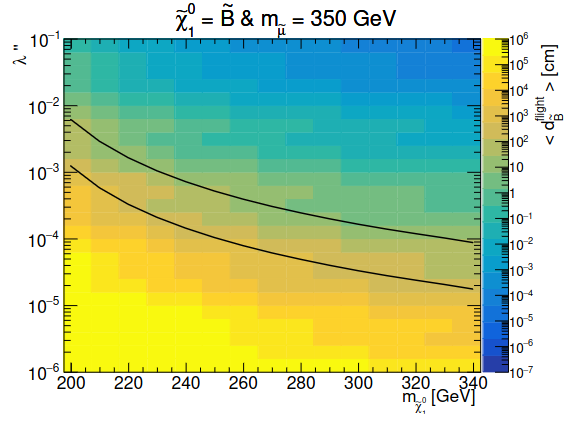
\includegraphics[height=6cm, width=8cm, trim= 0cm 0cm 0cm 0.cm,clip]{images/PhaseSPace/Meandecaylength.png}
\caption{\label{fig:bgctau} \textcolor{red}{to be replaced} Mean decay length of the neutralino as a function of the neutralino mass and coupling. The black lines are the limits of the volume of the tracker of CMS. The tracker volume sets constraints on the phase space to be probed.}
\end{figure}

The cross section $\sigma$ of the pair production of $\Tilde{\mu}$ is displayed in Tables~\ref{tab:RLLRXS}, \ref{tab:LEFTXS} and~\ref{tab:RIGHTXS} for different mixing of left- and right-handed sleptons at Run 2 and in Tables~\ref{tab:RLLRXS13p6}, \ref{tab:LEFTXS13p6} and~\ref{tab:RIGHTXS13p6} at Run 3 . For simplicity all other RPV couplings are null. 
%\\

%\FloatBarrier
\begin{table}
    \centering
    \begin{tabular}{ | c | c | c |}
        \hline
        \rowcolor{lightgray} 
         $m_{\Tilde{\mu}}$ [GeV] &  LO [fb] & LO + 1 jet [fb]\\
         \hline
         200  & $8.964^{+1.71\%}_{-1.86\%} \pm 1.83\%$ & $14.35^{+5.72\%}_{-4.41\%} \pm 1.92\%$ \\
         \hline
         250   & $3.776^{+2.88\%}_{-2.86\%} \pm 2.13\%$ &  $6.25^{+5.90\%}_{-4.57\%} \pm 2.14\%$\\
         \hline
         300  & $1.8158^{+3.87\%}_{-3.69\%} \pm 2.36\%$ &  $3.06^{+5.94\%}_{-4.67\%} \pm 2.50\%$\\
         \hline
         350 &  $0.9484^{+4.65\%}_{-4.34\%} \pm 2.66\%$ &  $1.64^{+6.08\%}_{-4.75\%} \pm 2.75\%$\\
         \hline
         400  & $0.5292^{+5.37\%}_{-4.93\%} \pm 2.93\%$ & $0.94^{+6.27\%}_{-4.89\%} \pm 3.17\%$\\
         \hline
         450  & $0.3102^{+5.99\%}_{-5.43\%} \pm 3.17\%$ & $0.55^{+6.20\%}_{-5.47\%} \pm 3.33\%$\\
         \hline
         500  & $0.18886^{+6.57\%}_{-5.9\%} \pm 3.49\%$ & $0.34^{+6.65\%}_{-5.98\%} \pm 3.57\%$\\
         \hline
    \end{tabular}
    \caption{Total production cross sections at pp center-of-mass energy of 13 TeV, for second generation mixed states (50\% right-handed, 50\% left-handed) sleptons. Results are given in fb with the associated uncertainties using the PDF PDF4LHC15\_nlo\_mc (LHAid : 90500). The second column gives the cross sections at LO obtained with MADGRAPH5\_aMC@NLO for this analysis, the third column is at LO + 1 jet. Asymmetric uncertainties are scale variations while symmetric variations are PDF uncertainties.} 
    \label{tab:RLLRXS}
\end{table}

\begin{table}
    \centering
    \begin{tabular}{ | c | c |}
        \hline
        \rowcolor{lightgray} 
         $m_{\Tilde{\mu}}$ [GeV] &  LO + 1 jet [fb]\\
         \hline
         200  & $15.59^{+5.80\%}_{-4.47\%} \pm 1.86\%$  \\
         \hline
         250   & $6.86^{+5.94\%}_{-4.60\%} \pm 2.03\%$ \\
         \hline
         300  & $3.39^{+6.07\%}_{-4.71\%} \pm 2.43\%$ \\
         \hline
         350 &  $1.82^{+6.21\%}_{-4.83\%} \pm 2.69\%$\\
         \hline
         400  & $1.04^{+6.28\%}_{-4.90\%} \pm 3.21\%$ \\
         \hline
         450  & $0.62^{+6.33\%}_{-4.95\%} \pm 3.20\%$ \\
         \hline
         500  & $0.39^{+6.36\%}_{-4.93\%} \pm 3.41\%$ \\
         \hline
    \end{tabular}
    \caption{Total production cross sections at pp center-of-mass energy of 13.6 TeV, for second generation mixed states (50\% right-handed, 50\% left-handed) sleptons. Results are given in fb with the associated uncertainties using the PDF PDF4LHC15\_nlo\_mc (LHAid : 90500). The second column gives the cross sections at LO + 1 jet obtained with MADGRAPH5\_aMC@NLO for this analysis. Asymmetric uncertainties are scale variations while symmetric variations are PDF uncertainties.} 
    \label{tab:RLLRXS13p6}
\end{table}

\begin{table}
    \centering
    \begin{tabular}{ | c || c | m{6em} | c |}
        \hline
        \rowcolor{lightgray} 
         $m_{\Tilde{\mu}}$ [GeV]  & LO [fb] this analysis & LO [fb] \cite{Fuks_2014}& LO [fb] \cite{Fiaschi_2018}\\
         \hline
         \hline
         200 & $17.93^{+1.69\%}_{-1.85\%} \pm 1.87\%$  & $18.84^{+1.3\%}_{-1.6\%}$ & $18.68^{+0.8\%}_{-1.1\%} \pm 6.2\%$ \\
         \hline
         250  & $7.55^{+2.88\%}_{-2.86\%} \pm 2.16\% $   & $8.04^{+2.8\%}_{-2.9\%}$  & $8.14^{+2.2\%}_{-2.4\%} \pm 6.2\%$  \\
         \hline
         300  & $3.63^{+3.87\%}_{-3.69\%} \pm 2.36\%$ & $3.89^{+4.0\%}_{-3.8\%}$  & $4.01^{+3.4\%}_{-3.3\%} \pm 6.2\%$ \\
         \hline
         350  & $1.9^{+4.65\%}_{-4.33\%} \pm 2.67\%$  & $2.05^{+4.9\%}_{-4.6\%}$  & $2.15^{+4.3\%}_{-4.1\%} \pm 6.2\%$ \\
         \hline
         400   & $1.06^{+5.37\%}_{-4.93\%} \pm 2.93\%$ & $1.15^{+5.7\%}_{-5.2\%}$   & $1.23^{+5.1\%}_{-4.8\%} \pm 6.2\%$ \\
         \hline
         450   & $0.62^{+5.98\%}_{-5.42\%} \pm 3.16\%$   & $0.68^{+6.4\%}_{-5.8\%}$  & $0.74^{+5.8\%}_{-5.3\%} \pm 6.3\%$ \\
         \hline
         500  & $0.38^{+6.56\%}_{-5.89\%} \pm 3.47\%$   & $0.42^{+7.1\%}_{-6.3\%}$  & $0.46^{+6.5\%}_{-5.8\%} \pm 6.4\%$ \\
         \hline
    \end{tabular}
    \caption{Total production cross sections at pp center-of-mass  energy of 13 TeV, for second generation left-handed sleptons. Results are given in fb with the associated uncertainties using the PDF PDF4LHC15\_nlo\_mc (LHAid : 90500). The second column gives the cross sections obtained with MADGRAPH5\_aMC@NLO for this analysis. The third column is from~\cite{Fuks_2014} and the fourth column from~\cite{Fiaschi_2018}. The cross sections could be extended at NLO using a $K$ factor ($\frac{\sigma_{NLO}}{\sigma_{LO}}$) of about 1.4. Asymmetric uncertainties are scale variations while symmetric variations are PDF uncertainties.} 
    \label{tab:LEFTXS}
\end{table}

\begin{table}
    \centering
    \begin{tabular}{ | c || c |}
        \hline
        \rowcolor{lightgray} 
         $m_{\Tilde{\mu}}$ [GeV]  & LO + 1 jet [fb] \\
         \hline
         \hline
         200 & $31.17^{+5.80\%}_{-4.47\%} \pm 1.86\%$  \\
         \hline
         250  & $13.73^{+5.94\%}_{-4.60\%} \pm 2.03\% $   \\
         \hline
         300  & $6.77^{+6.07\%}_{-4.71\%} \pm 2.43\%$ \\
         \hline
         350  & $3.65^{+6.21\%}_{-4.84\%} \pm 2.69\%$ \\
         \hline
         400   & $2.09^{+6.28\%}_{-4.90\%} \pm 3.21\%$ \\
         \hline
         450   & $1.25^{+6.33\%}_{-5.27\%} \pm 3.20\%$  \\
         \hline
         500  & $0.78^{+6.65\%}_{-5.75\%} \pm 3.41\%$  \\
         \hline
    \end{tabular}
    \caption{Total production cross sections at pp center-of-mass  energy of 13.6 TeV, for second generation left-handed sleptons. Results are given in fb with the associated uncertainties using the PDF PDF4LHC15\_nlo\_mc (LHAid : 90500). The second column gives the cross sections obtained with MADGRAPH5\_aMC@NLO for this analysis. The third column is from~\cite{Fuks_2014} and the fourth column from~\cite{Fiaschi_2018}. The cross sections could be extended at NLO using a $K$ factor ($\frac{\sigma_{NLO}}{\sigma_{LO}}$) of about 1.4. Asymmetric uncertainties are scale variations while symmetric variations are PDF uncertainties.} 
    \label{tab:LEFTXS13p6}
\end{table}

\begin{table}
    \centering
    \begin{tabular}{ | c || c | m{6em} |}
        \hline
        \rowcolor{lightgray} 
         $m_{\Tilde{\mu}}$ [GeV]  & LO [fb] this analysis & LO [fb] \cite{Fuks_2014} \\
         \hline
         \hline
         200 & $7.66^{+1.63\%}_{-1.8\%} \pm 2.11\% $  & $7.03^{+1.3\%}_{-1.6\%}$  \\
         \hline
         250  & $3.25^{+2.82\%}_{-2.8\%} \pm 2.28\%$   & $3.03^{+2.8\%}_{-2.9\%}$  \\
         \hline
         300  & $1.57^{+3.8\%}_{-3.63\%} \pm 2.47\%$ & $1.48^{+4.0\%}_{-3.8\%}$  \\
         \hline
         350  & $0.83^{+4.61\%}_{-4.3\%} \pm 2.76\% $  & $0.78^{+4.8\%}_{-4.5\%}$  \\
         \hline
         400   & $0.46^{+5.3\%}_{-4.87\%} \pm 2.94\%$ & $0.44^{+5.7\%}_{-5.2\%}$ \\
         \hline
         450   & $0.27^{+5.89\%}_{-5.35\%} \pm 3.2\%$   & $0.26^{+6.4\%}_{-5.7\%}$  \\
         \hline
         500  & $0.17^{+6.47\%}_{-5.82\%} \pm 3.46\%$   & $0.16^{+7.0\%}_{-6.2\%}$ \\
         \hline
    \end{tabular}
    \caption{Total production cross sections at pp center-of-mass  energy of 13 TeV, for second generation right-handed sleptons. Results are given in fb with the associated uncertainties using the PDF PDF4LHC15\_nlo\_mc (LHAid : 90500). The second column gives the cross sections obtained with MADGRAPH5\_aMC@NLO for this analysis, the third column is from~\cite{Fuks_2014}. The cross sections can be extended at NLO using a $K$ factor ($\frac{\sigma_{NLO}}{\sigma_{LO}}$) of about 1.4. Asymmetric uncertainties are scale variations and symmetric uncertainties are PDF variations.} 
    \label{tab:RIGHTXS}
\end{table}

\begin{table}
    \centering
    \begin{tabular}{ | c || c |}
        \hline
        \rowcolor{lightgray} 
         $m_{\Tilde{\mu}}$ [GeV]  & LO + 1 jet [fb]  \\
         \hline
         \hline
         200 & $13.36^{+5.86\%}_{-4.51\%} \pm 2.07\% $  \\
         \hline
         250  & $5.92^{+5.93\%}_{-4.59\%} \pm 2.27\%$    \\
         \hline
         300  & $2.94^{+6.18\%}_{-4.80\%} \pm 2.53\%$  \\
         \hline
         350  & $1.59^{+6.21\%}_{-4.83\%} \pm 2.76\% $   \\
         \hline
         400   & $0.91^{+6.31\%}_{-4.83\%} \pm 3.00\%$  \\
         \hline
         450   & $0.55^{+6.34\%}_{-5.22\%} \pm 3.27\%$   \\
         \hline
         500  & $0.34^{+6.39\%}_{-5.67\%} \pm 3.55\%$  \\
         \hline
    \end{tabular}
    \caption{Total production cross sections at pp center-of-mass  energy of 13.6 TeV, for second generation right handed sleptons. Results are given in fb with the associated uncertainties using the PDF PDF4LHC15\_nlo\_mc (LHAid : 90500). The second column gives the cross sections obtained with MADGRAPH5\_aMC@NLO for this analysis, the third column is from~\cite{Fuks_2014}. The cross sections can be extended at NLO using a $K$ factor ($\frac{\sigma_{NLO}}{\sigma_{LO}}$) of about 1.4. Asymmetric uncertainties are scale variations and symmetric uncertainties are PDF variations.} 
    \label{tab:RIGHTXS13p6}
\end{table}
%\FloatBarrier


\subsection{Background}

 The background sources for this displaced vertices search are mainly $t\Bar{t}$ and Drell-Yan.
To develop the analysis, MC samples generated during the Summer20 Ultra-Legacy campaign for 2016, 2017 and 2018 stored in the MiniAODv2 format are used. The CMSSW settings to process these MC samples are given in Table [\ref{tab:MCSET}] for Run 2 and Table \ref{tab:MCSETRun3} .
These samples are listed for each year of Run 2 in the Tables [\ref{tab:MC2016}], [\ref{tab:MC2017}] and [\ref{tab:MC2018}].

\begin{table}
    \centering
    \begin{tabular}{| c | c | c |}
    \hline
    \rowcolor{lightgray} 
         Year &  CMSSW release & Global Tag  \\
    \hline
         2016Pre & 10\_6\_30&   106X\_mcRun2\_asymptotic\_preVFP\_v11\\
    \hline
         2016Post & 10\_6\_30 &  106X\_mcRun2\_asymptotic\_v17  \\
    \hline
         2017 & 10\_6\_30 &  106X\_mc2017\_realistic\_v10  \\
    \hline
         2018 & 10\_6\_30  &  106X\_upgrade2018\_realistic\_v16\_L1v1 \\
    \hline
    \end{tabular}
    \caption{Version of the CMS Software and the associated global tag for each year of Run 2}
    \label{tab:MCSET}
\end{table}

\begin{table}
    \centering
    \begin{tabular}{| c | c | c |}
    \hline
    \rowcolor{lightgray} 
         Year &  CMSSW release & Global Tag  \\
    \hline
         2022 & 14\_0\_8 &   130X\_mcRun3\_2022\_realistic\_v5\\
    \hline
         2022EE & 14\_0\_8 &  130X\_mcRun3\_2022\_realistic\_postEE\_v6  \\
    \hline
         2023 & 14\_0\_8 &  130X\_mcRun3\_2023\_realistic\_v14  \\
    \hline
         2023BPix & 14\_0\_8 &   130X\_mcRun3\_2023\_realistic\_postBPix\_v2 \\
    \hline
    \end{tabular}
    \caption{Version of the CMS Software and the associated global tag for each year of Run 3}
    \label{tab:MCSETRun3}
\end{table}


\begin{table}[h]
\centering
\begin{tabular}{|c|c|c|}
  \hline
  \rowcolor{lightgray} 
  Sample 2016 & No. events & $\sigma$ [pb] \\
  \hline
  \footnotesize/TTTo2L2Nu\_TuneCP5\_13TeV-powheg-pythia8                                   & 960000 & 88.3\\
  \footnotesize /ST\_tW\_top\_5f\_NoFullyHadronicDecays\_TuneCP5\_13TeV-powheg-pythia8     & 963768 &  10.8908 \\
  \footnotesize /ST\_tW\_antitop\_5f\_NoFullyHadronicDecays\_TuneCP5\_13TeV-powheg-pythia8 & 920153 & 10.8707 \\
  \footnotesize/DYJetsToLL\_M-10to50\_TuneCP5\_13TeV-madgraphMLM-pythia8                   & 1836747 & 15910.0\\
  \footnotesize/DYJetsToLL\_M-50\_TuneCP5\_13TeV-madgraphMLM-pythia8                       & 800000 & 5379\\
  \footnotesize/WWTo2L2Nu\_TuneCP5\_13TeV-powheg-pythia8                                   & 780000 & 11.09\\
  \footnotesize/WZTo2Q2L\_mllmin4p0\_TuneCP5\_13TeV-amcatnloFXFX-pythia8                   & 994094 & 6.535\\
  \footnotesize/ZZTo2Q2L\_mllmin4p0\_TuneCP5\_13TeV-amcatnloFXFX-pythia8                   &  780170 & 3.676 \\
  \footnotesize/ttWJetsToLNu\_5f\_EWK\_TuneCP5\_13TeV\_amcatnlo-pythia8                    & 825000 & 0.290 \\
  \footnotesize/TTZToLL\_5f\_TuneCP5\_13TeV-madgraphMLM-pythia8                            & 660694 & 0.05188\\
  \footnotesize/TTWW\_TuneCP5\_13TeV-madgraph-pythia8                                      & 570000 &  0.006992\\

  \hline
\end{tabular}
    \caption{Background MC samples fro 2016 with their associated number of events and cross-sections}
    \label{tab:MC2016}
\end{table}
\FloatBarrier
\begin{table}[h]
\centering
\begin{tabular}{|c|c|c|}
  \hline
  \rowcolor{lightgray} 
  Sample 2017 & No. events & $\sigma$ [pb] \\
  \hline
  \footnotesize/TTTo2L2Nu\_TuneCP5\_13TeV-powheg-pythia8 & 960000 & 88.3\\
  \footnotesize /ST\_tW\_top\_5f\_NoFullyHadronicDecays\_TuneCP5\_13TeV-powheg-pythia8 & 963768 &  10.8908 \\
  \footnotesize /ST\_tW\_antitop\_5f\_NoFullyHadronicDecays\_TuneCP5\_13TeV-powheg-pythia8 & 920153 & 10.8707 \\
  \footnotesize/DYJetsToLL\_M-10to50\_TuneCP5\_13TeV-madgraphMLM-pythia8 & 1836747 & 15910.0\\
  \footnotesize/DYJetsToLL\_M-50\_TuneCP5\_13TeV-madgraphMLM-pythia8 & 800000 & 5379\\
  \footnotesize/WWTo2L2Nu\_TuneCP5\_13TeV-powheg-pythia8 & 780000 & 11.09\\
  \footnotesize/WZTo2Q2L\_mllmin4p0\_TuneCP5\_13TeV-amcatnloFXFX-pythia8 & 994094 & 6.535\\
  \footnotesize/ZZTo2Q2L\_mllmin4p0\_TuneCP5\_13TeV-amcatnloFXFX-pythia8 &  780170 & 3.676 \\
  \footnotesize/ttWJetsToLNu\_5f\_EWK\_TuneCP5\_13TeV\_amcatnlo-pythia8 & 825000 & 0.290 \\
  \footnotesize/TTZToLL\_5f\_TuneCP5\_13TeV-madgraphMLM-pythia8 & 660694 & 0.05188\\
  \footnotesize/TTWW\_TuneCP5\_13TeV-madgraph-pythia8  & 570000 &  0.006992\\

  \hline
\end{tabular}
    \caption{Background MC samples for 2017 with their associated number of events and cross-sections}
    \label{tab:MC2017}
\end{table}
\FloatBarrier
\begin{table}[h]
\centering
\begin{tabular}{|c|c|c|}
  \hline
  \rowcolor{lightgray} 
  Sample 2018 & No. events & $\sigma$ [pb] \\
  \hline
  \footnotesize/TTTo2L2Nu\_TuneCP5\_13TeV-powheg-pythia8 & 960000 & 88.3\\
  \footnotesize /ST\_tW\_top\_5f\_NoFullyHadronicDecays\_TuneCP5\_13TeV-powheg-pythia8 & 963768 &  10.8908 \\
  \footnotesize /ST\_tW\_antitop\_5f\_NoFullyHadronicDecays\_TuneCP5\_13TeV-powheg-pythia8 & 920153 & 10.8707 \\
  \footnotesize/DYJetsToLL\_M-10to50\_TuneCP5\_13TeV-madgraphMLM-pythia8 & 1836747 & 15910.0\\
  \footnotesize/DYJetsToLL\_M-50\_TuneCP5\_13TeV-madgraphMLM-pythia8 & 800000 & 5379\\
  \footnotesize/WWTo2L2Nu\_TuneCP5\_13TeV-powheg-pythia8 & 780000 & 11.09\\
  \footnotesize/WZTo2Q2L\_mllmin4p0\_TuneCP5\_13TeV-amcatnloFXFX-pythia8 & 994094 & 6.535\\
  \footnotesize/ZZTo2Q2L\_mllmin4p0\_TuneCP5\_13TeV-amcatnloFXFX-pythia8 &  780170 & 3.676 \\
  \footnotesize/ttWJetsToLNu\_5f\_EWK\_TuneCP5\_13TeV\_amcatnlo-pythia8 & 825000 & 0.290 \\
  \footnotesize/TTZToLL\_5f\_TuneCP5\_13TeV-madgraphMLM-pythia8 & 660694 & 0.05188\\
  \footnotesize/TTWW\_TuneCP5\_13TeV-madgraph-pythia8  & 570000 &  0.006992\\

  \hline
\end{tabular}
    \caption{Background MC samples for 2018 with their associated number of events and cross-sections}
    \label{tab:MC2018}
\end{table}
\FloatBarrier
%%%%%%%%%%%%%%%%%%%%%%%%%%%%%%%%%%%%%%%%%%%%%%%%%%%%%%%%%%%%%%%
%%%%%%%%%%%%%%%%%%%%%%%%%%%%%%%%%%%%%%%%%%%%%%%%%%%%%%%%%%%%%%%
%------------------- SECTION ----------------------------------
%%%%%%%%%%%%%%%%%%%%%%%%%%%%%%%%%%%%%%%%%%%%%%%%%%%%%%%%%%%%%%%
%%%%%%%%%%%%%%%%%%%%%%%%%%%%%%%%%%%%%%%%%%%%%%%%%%%%%%%%%%%%%%%


\section{Datasets}
\label{SEC: DATASET}
\subsection{Run 2}
Since the experimental signature has two prompt muons, this analysis makes use of one data sample :
\begin{itemize}
    \item DoubleMuon
\end{itemize}
% For the electron channel : 
% \begin{itemize}
%     \item SingleElectron, called EGamma in 2018
%     \item DoubleElectron
% \end{itemize}

The trigger set is given in Table\ref{tab:TRIGGER2016} for 2016, Table\ref{tab:TRIGGER2017} for 2017 and in Table.\ref{tab:TRIGGER2018} for 2018. 

\begin{table}[h]
\centering
\begin{tabular}{|c|p{12cm}|}
  \hline
  \rowcolor{lightgray} 
  Dataset & Trigger \\
  % \hline
  % SingleMuon & HLT\_IsoMu27\_v \textbf{OR}  HLT\_IsoTkMu24\_v\\
  \hline
  DoubleMuon & HLT\_Mu17\_TrkIsoVVL\_Mu8\_TrkIsoVVL\_DZ\_v \textbf{OR} HLT\_Mu17\_TrkIsoVVL\_TkMu8\_TrkIsoVVL\_DZ\_v \textbf{OR} HLT\_Mu17\_TrkIsoVVL\_Mu8\_TrkIsoVVL\_v  \\
  \hline
\end{tabular}
    \caption{Trigger for the datasets of 2016}
    \label{tab:TRIGGER2016}
\end{table}

\begin{table}[h]
\centering
\begin{tabular}{|c|p{13 cm}|}
  \hline
  \rowcolor{lightgray} 
  Dataset & Trigger \\
  % \hline
  % SingleMuon & HLT\_IsoMu24\_v\\
  \hline
  DoubleMuon & HLT\_Mu17\_TrkIsoVVL\_Mu8\_TrkIsoVVL\_DZ\_Mass3p8\_v \textbf{OR} HLT\_Mu17\_TrkIsoVVL\_Mu8\_TrkIsoVVL\_DZ\_Mass8\_v \\
  \hline
\end{tabular}
    \caption{Trigger for the datasets of 2017}
    \label{tab:TRIGGER2017}
\end{table}



\begin{table}[h]
\centering
\begin{tabular}{|c|p{13 cm}|}
  \hline
  \rowcolor{lightgray} 
  Dataset & Trigger \\
  % \hline
  % SingleMuon & HLT\_IsoMu24\_v\\
  \hline
  DoubleMuon & HLT\_Mu17\_TrkIsoVVL\_Mu8\_TrkIsoVVL\_DZ\_Mass3p8\_v \textbf{OR} HLT\_Mu17\_TrkIsoVVL\_Mu8\_TrkIsoVVL\_DZ\_Mass8\_v\\
  \hline
\end{tabular}
    \caption{Trigger for the datasets of 2018}
    \label{tab:TRIGGER2018}
\end{table}

\begin{table}
    \centering
    \begin{tabular}{| c | c | c |}
    \hline
    \rowcolor{lightgray} 
         Year &  Global Tag & Golden JSON \\
    \hline
         2016Pre &  \scriptsize  106X\_dataRun2\_v37 & \scriptsize Cert\_271036-284044\_13TeV\_Legacy2016\_Collisions16\_JSON.txt\\
    \hline
         2016Post &  \scriptsize 106X\_dataRun2\_v37  & \scriptsize Cert\_271036-284044\_13TeV\_Legacy2016\_Collisions16\_JSON.txt \\
    \hline
         2017 &  \scriptsize 106X\_dataRun2\_v37 & \scriptsize Cert\_294927-306462\_13TeV\_UL2017\_Collisions17\_GoldenJSON.txt\\
    \hline
         2018 &  \scriptsize 106X\_dataRun2\_v37 & \scriptsize
         Cert\_314472-325175\_13TeV\_Legacy2018\_Collisions18\_JSON.txt\\
    \hline
    \end{tabular}
    \caption{Global tags with the associated Golden JSON file for each year of Run 2}
    \label{tab:DATASET}
\end{table}
\FloatBarrier

\subsection{Run 3}
The new muon datasets are used:
\begin{itemize}
    \item Muon for 2022
    \item Muon0 and Muon1 for 2023 and 2024
\end{itemize}

For each data set, the trigger set is given in Table\ref{tab:TRIGGER2022} for 2022, Table\ref{tab:TRIGGER2023} for 2023 and Table\ref{tab:TRIGGER2024} for 2024 with the associated Global tag in Table \ref{tab:DATASETRun3}. 

\begin{table}[h]
\centering
\begin{tabular}{|c|p{12cm}|}
  \hline
  \rowcolor{lightgray} 
  Dataset & Trigger \\
  % \hline
  % SingleMuon & HLT\_IsoMu27\_v \textbf{OR}  HLT\_IsoTkMu24\_v\\
  \hline
  DoubleMuon & HLT\_Mu17\_TrkIsoVVL\_Mu8\_TrkIsoVVL\_DZ\_v \textbf{OR} HLT\_Mu17\_TrkIsoVVL\_TkMu8\_TrkIsoVVL\_DZ\_v \textbf{OR} HLT\_Mu17\_TrkIsoVVL\_Mu8\_TrkIsoVVL\_v  \\
  \hline
\end{tabular}
    \caption{Trigger for the datasets of 2022}
    \label{tab:TRIGGER2022}
\end{table}

\begin{table}[h]
\centering
\begin{tabular}{|c|p{13 cm}|}
  \hline
  \rowcolor{lightgray} 
  Dataset & Trigger \\
  % \hline
  % SingleMuon & HLT\_IsoMu24\_v\\
  \hline
  DoubleMuon & HLT\_Mu17\_TrkIsoVVL\_Mu8\_TrkIsoVVL\_DZ\_Mass3p8\_v \textbf{OR} HLT\_Mu17\_TrkIsoVVL\_Mu8\_TrkIsoVVL\_DZ\_Mass8\_v \\
  \hline
\end{tabular}
    \caption{Trigger for the datasets of 2023}
    \label{tab:TRIGGER2023}
\end{table}



\begin{table}[h]
\centering
\begin{tabular}{|c|p{13 cm}|}
  \hline
  \rowcolor{lightgray} 
  Dataset & Trigger \\
  % \hline
  % SingleMuon & HLT\_IsoMu24\_v\\
  \hline
  DoubleMuon & HLT\_Mu17\_TrkIsoVVL\_Mu8\_TrkIsoVVL\_DZ\_Mass3p8\_v \textbf{OR} HLT\_Mu17\_TrkIsoVVL\_Mu8\_TrkIsoVVL\_DZ\_Mass8\_v\\
  \hline
\end{tabular}
    \caption{Trigger for the datasets of 2024}
    \label{tab:TRIGGER2024}
\end{table}

\FloatBarrier

\begin{table}
    \centering
    \begin{tabular}{| c | c | c |}
    \hline
    \rowcolor{lightgray} 
         Year &  Global Tag & Golden JSON \\
    \hline
         2022 &  \scriptsize  140X\_dataRun3\_v3 & \scriptsize Cert\_Collisions2022\_355100\_362760\_Golden.json\\
    \hline
         2023 &  \scriptsize 140X\_dataRun3\_v3 & \scriptsize Cert\_Collisions2023\_366442\_370790\_Golden.json\\
         
    \hline
         2024 &  \scriptsize 140X\_dataRun3\_HLT\_v3 & \scriptsize
         Cert\_Collisions2024\_378981\_384380\_Golden.json\\
    \hline
    \end{tabular}
    \caption{Global tags with the associated Golden JSON file for each year of Run 3}
    \label{tab:DATASETRun3}
\end{table}
\FloatBarrier
%%%%%%%%%%%%%%%%%%%%%%%%%%%%%%%%%%%%%%%%%%%%%%%%%%%%%%%%%%%%%%%
%%%%%%%%%%%%%%%%%%%%%%%%%%%%%%%%%%%%%%%%%%%%%%%%%%%%%%%%%%%%%%%
%------------------- SECTION ----------------------------------
%%%%%%%%%%%%%%%%%%%%%%%%%%%%%%%%%%%%%%%%%%%%%%%%%%%%%%%%%%%%%%%
%%%%%%%%%%%%%%%%%%%%%%%%%%%%%%%%%%%%%%%%%%%%%%%%%%%%%%%%%%%%%%%
\newpage
\section{Object Selection}
\label{SEC: OBJSEL}
    Particle-Flow \cite{CMS:2017yfk} is the algorithm used by the CMS experiment to reconstruct objects by using the information of all sub-detectors. Selections are applied on the following reconstructed objects: on muons for the muon channel and on both leptons when looking at the electron-muon channel (used for background estimation) and jets for all channels. The analysis looks for prompt leptons with potential displaced leptons coming from the decay of heavy-flavor hadrons from the decay channel of the neutralino. In addition, the prompt leptons can overlap with the displaced jets, increasing the complexity of the experimental signature of the signal. All these constraints have been taken into account for the selections of the different objects and of the events.
    \subsection{Muons}
        Muons are reconstructed using the information from the tracker and the muon chambers. In this analysis, muons are required to be in the acceptance of the muon detector,$|\eta| <$ 2.4. All muons are required to have a $p_T > $  3 GeV. In the muon channel, there are two prompt muons that come from the decay of the smuons. These prompt muons are required to have constraints on their impact parameters, to be of opposite charge and also to follow the muon ID and isolation given in the Table.\ref{tab:MUONSEL}. The two prompt muons from the signal tend to be more energetic than muons from the Standard Model $t\bar{t}$ muons as shown in Fig.\ref{fig:MuonPt}. As the prompt signal muons come from the decay of the smuons, they also tend to be more back-to-back than $t\bar{t}$ muons as shown in Fig.\ref{fig:MuondR}.

        \begin{figure}[ht]
\centering
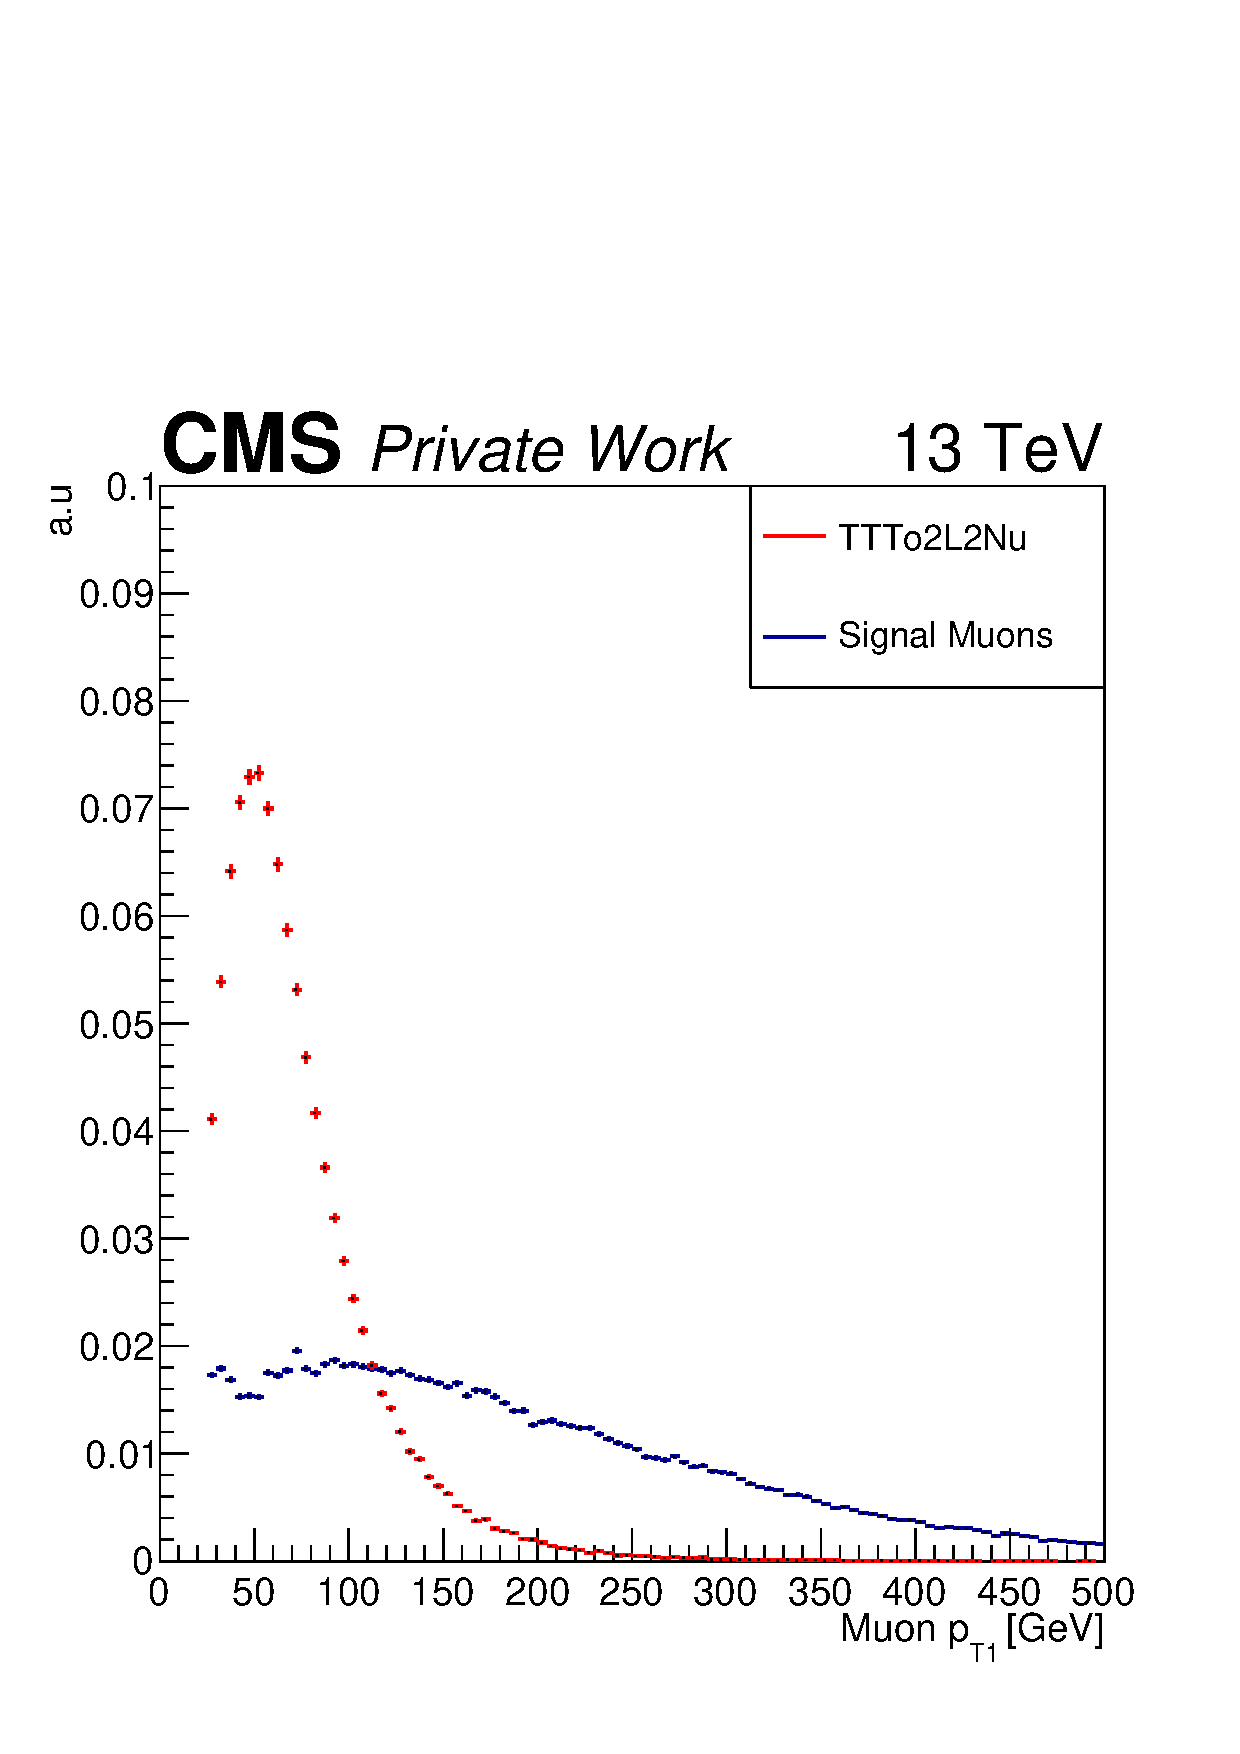
\includegraphics[height=8cm, width=8cm, trim= 0cm 0cm 0cm 0.cm,clip]{images/Muon/MuonLeadingPt.pdf}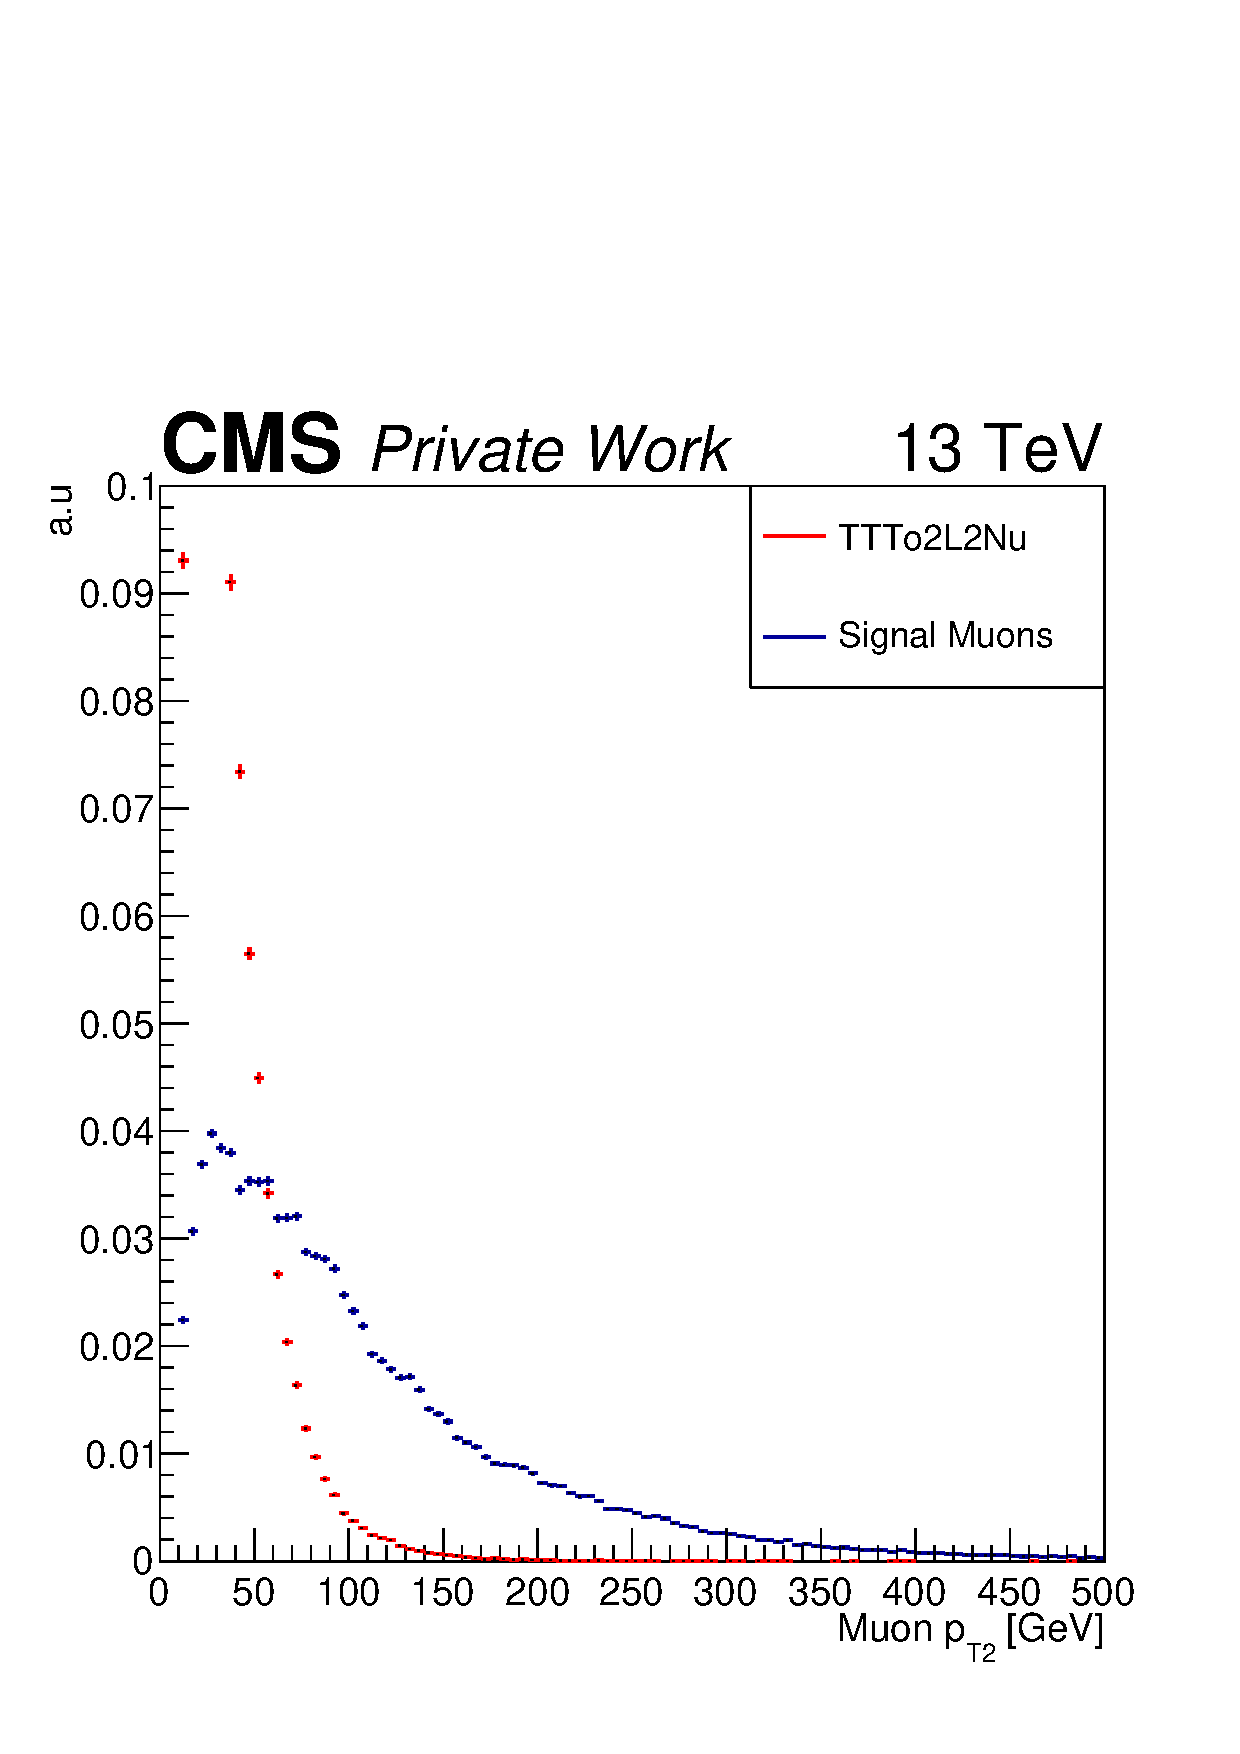
\includegraphics[height=8cm, width=8cm, trim= 0cm 0cm 0cm 0.cm,clip]{images/Muon/MuonLeadingPt2.pdf}
\caption{\label{fig:MuonPt} Distributions of the leading and sub-leading muon $p_T$ in signal events and $t\bar{t}$ MC events.}
\end{figure}
\FloatBarrier


        \begin{figure}[ht]
\centering
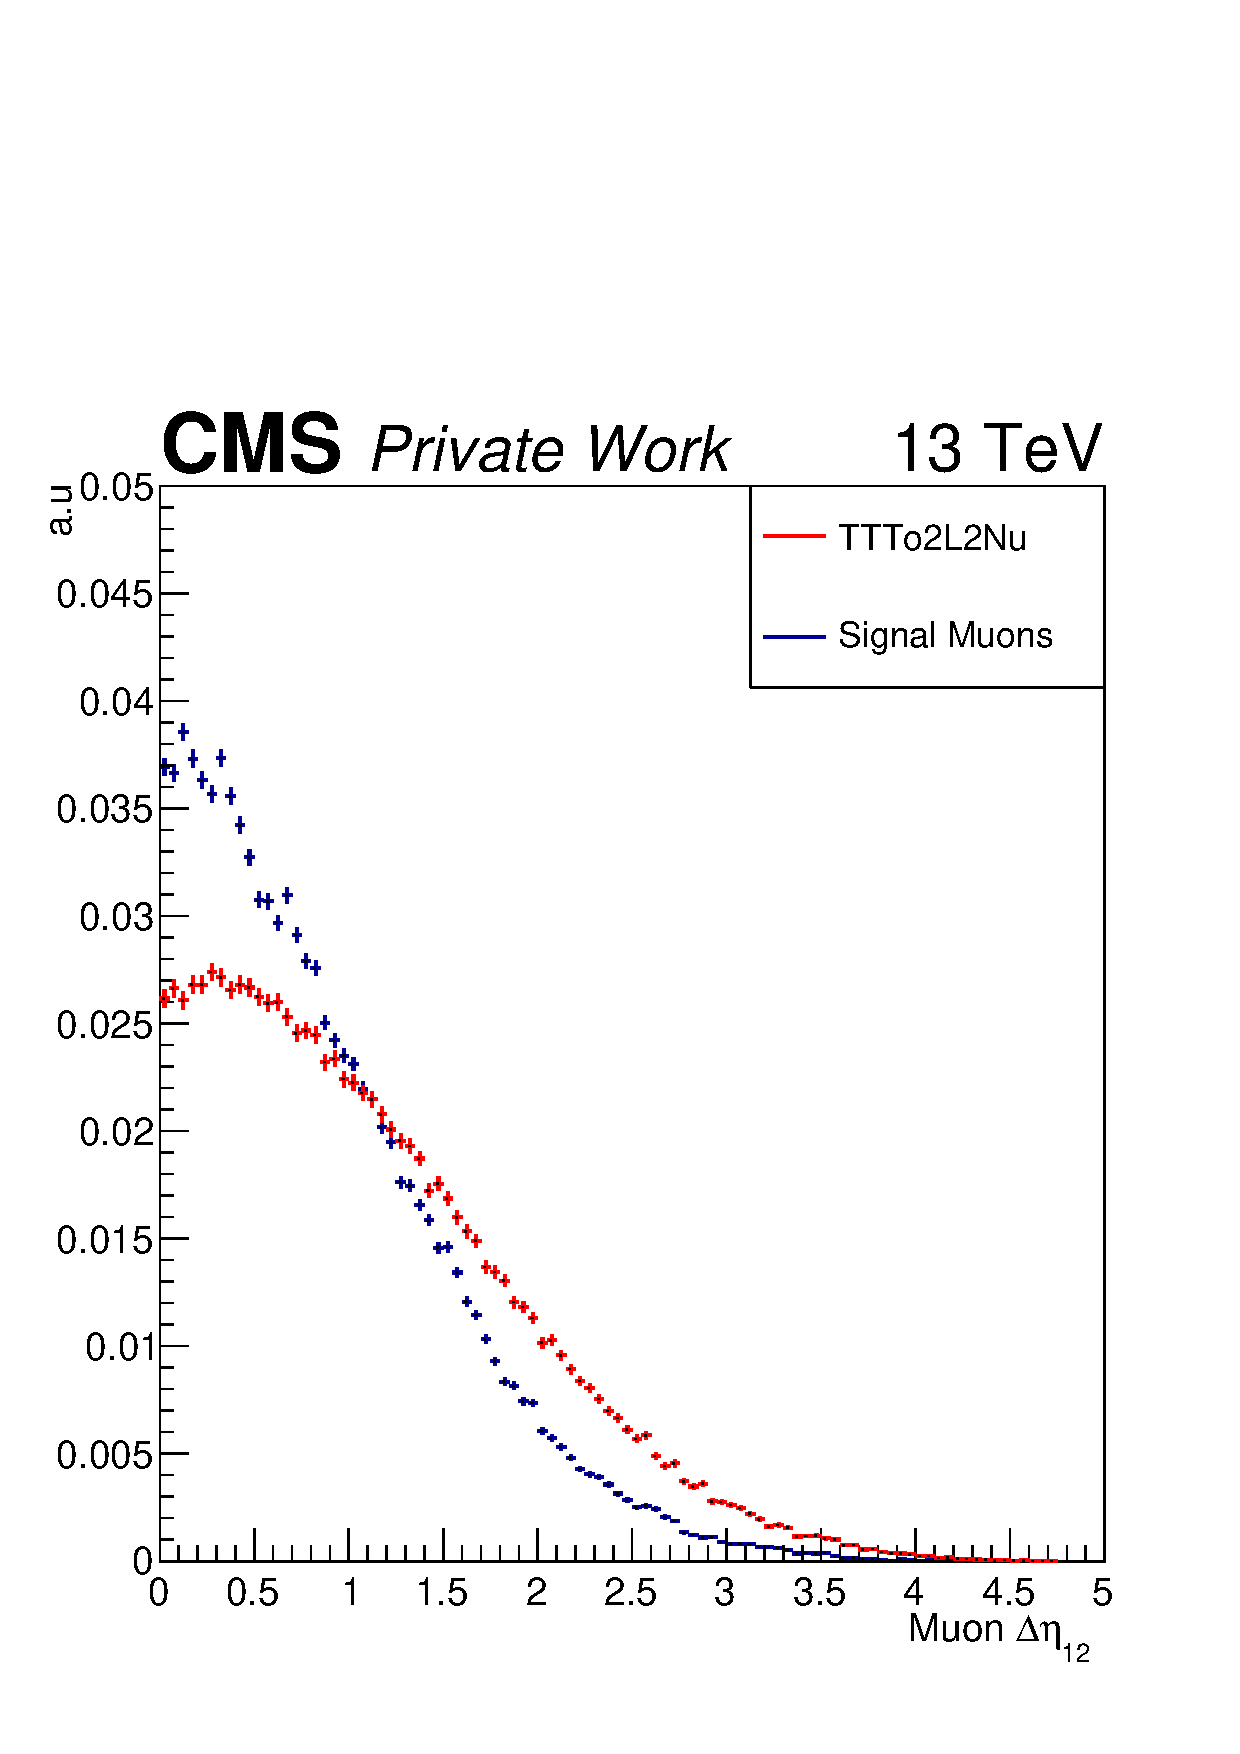
\includegraphics[height=8cm, width=8cm, trim= 0cm 0cm 0cm 0.cm,clip]{images/Muon/MuonMuondEta.pdf}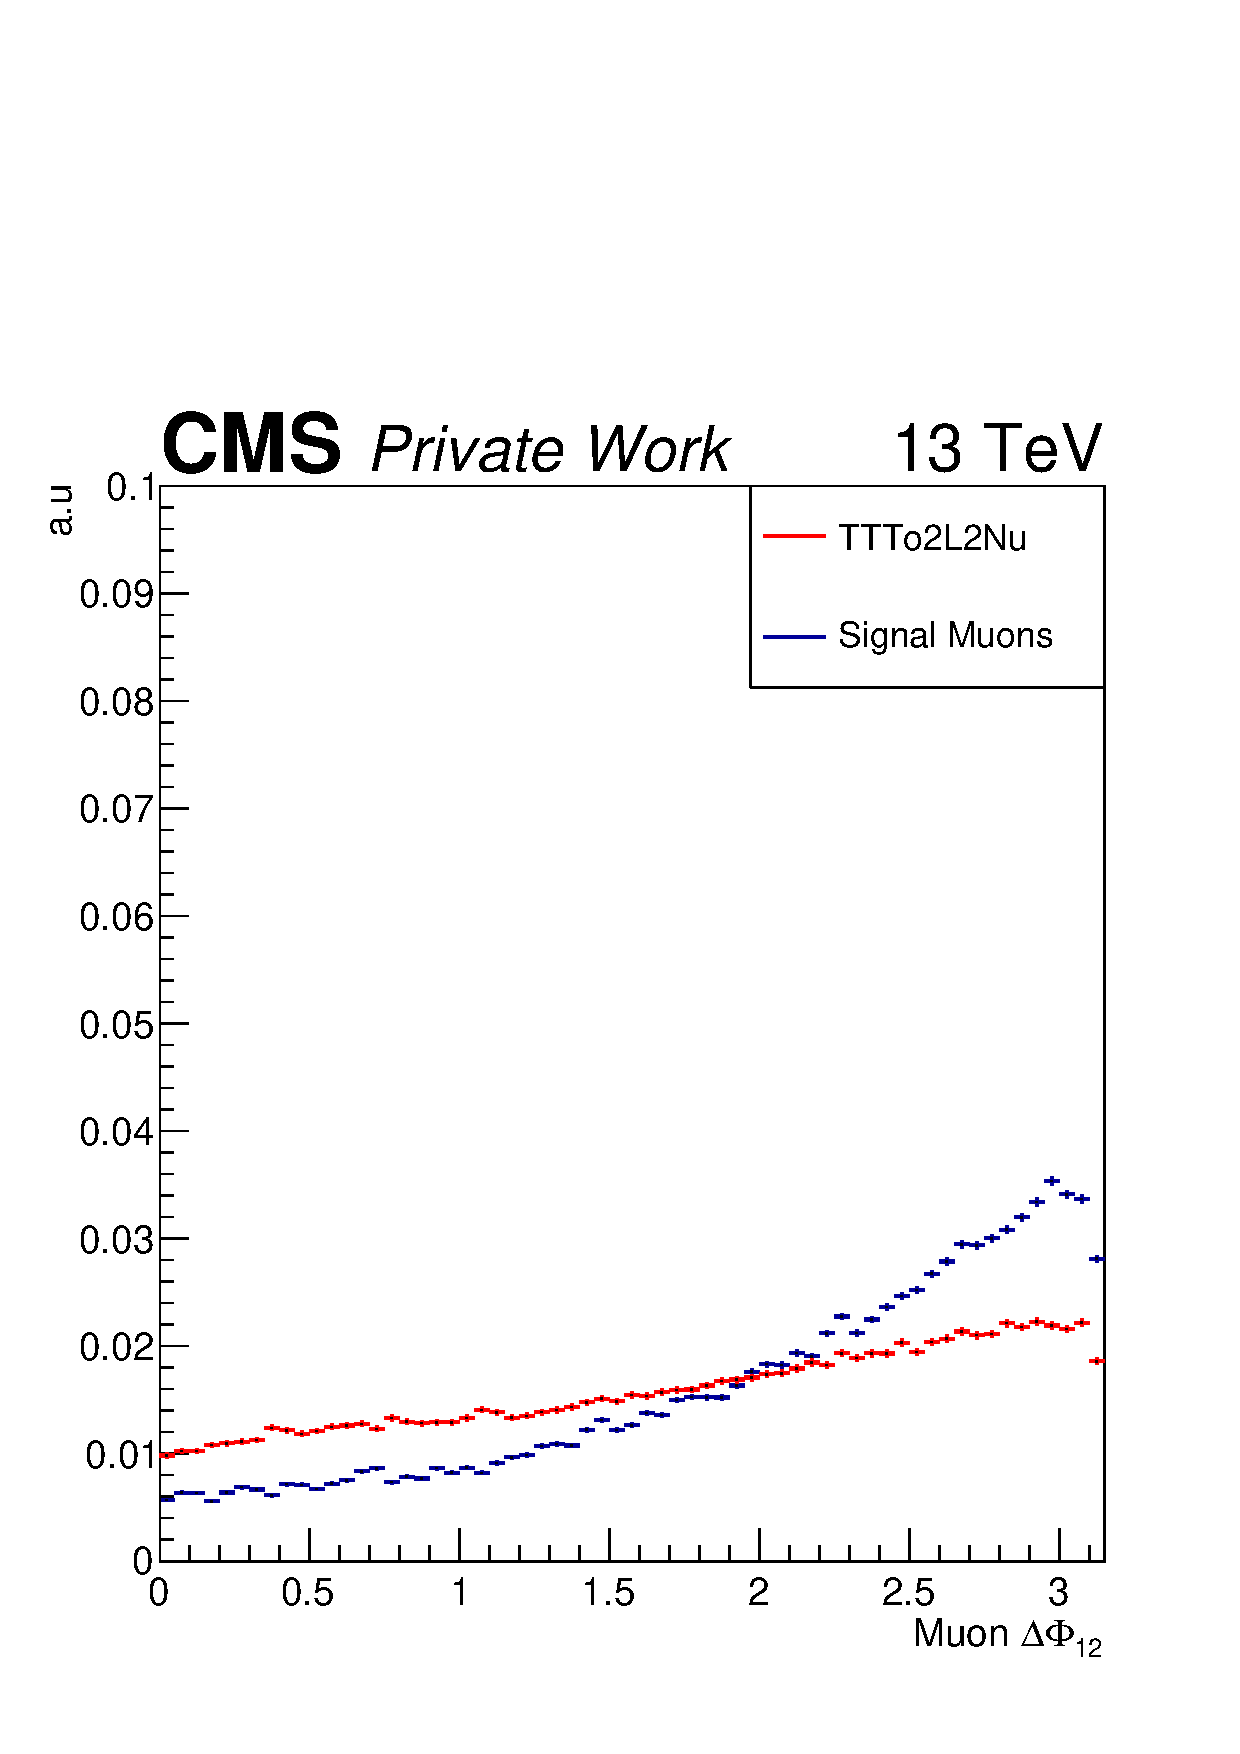
\includegraphics[height=8cm, width=8cm, trim= 0cm 0cm 0cm 0.cm,clip]{images/Muon/MuonMuondPhi.pdf}
\caption{\label{fig:MuondR} $\Delta\eta$ and $\Delta\phi$ distributions between the leading and sub-leading muon in signal events and $t\bar{t}$ MC events.}
\end{figure}
\FloatBarrier

\begin{table}[h]
\centering
\begin{tabular}{|c|c|c|}
  \hline
  \rowcolor{lightgray} 
  Selection & Prompt & Other \\
  \hline
  GlobalMuon & True & True\\
  $|\eta|$ & 2.4 & 2.4\\
  $p_T$ & 3 & 3\\
  $|d_{dxy}|$ & 0.1 cm & none\\
  $|d_{dz}|$ & 0.2 cm & none\\
  TightID & True & False\\
  MiniIsoTight & True & False\\
  \hline
\end{tabular}
    \caption{Selections for the Muons in the muon channel. The identification tag Tight refers to the recommendation tag of the MuonPOG \cite{MuonIDRun2} as well as the isolation flag MiniIsoTight. 
    \label{tab:MUONSEL}}
\end{table}


Concerning muon corrections, the Rochester Correction \cite{ROCCOR} have been applied on the Monte Carlo samples according to the Muon POG recommendations in order to correct the momentum scale and resolution of muons for each year of Run 2.

    In addition to the Rochester Correction, the scale factors for the muons are computed according to the Muon POG \cite{MuonSpark1}\cite{MuonSpark2} using the Spark T\&P tool for both Run 2 and Run 3. This tool is used to correct the discrepancy between data and MC for the muons but also for the trigger used (only for the muon channel). Scale factors are given in bins of $p_T$ and $\eta$ in Fig.\ref{fig:SP1}.
    \label{Spark}

\begin{figure}
    \centering
    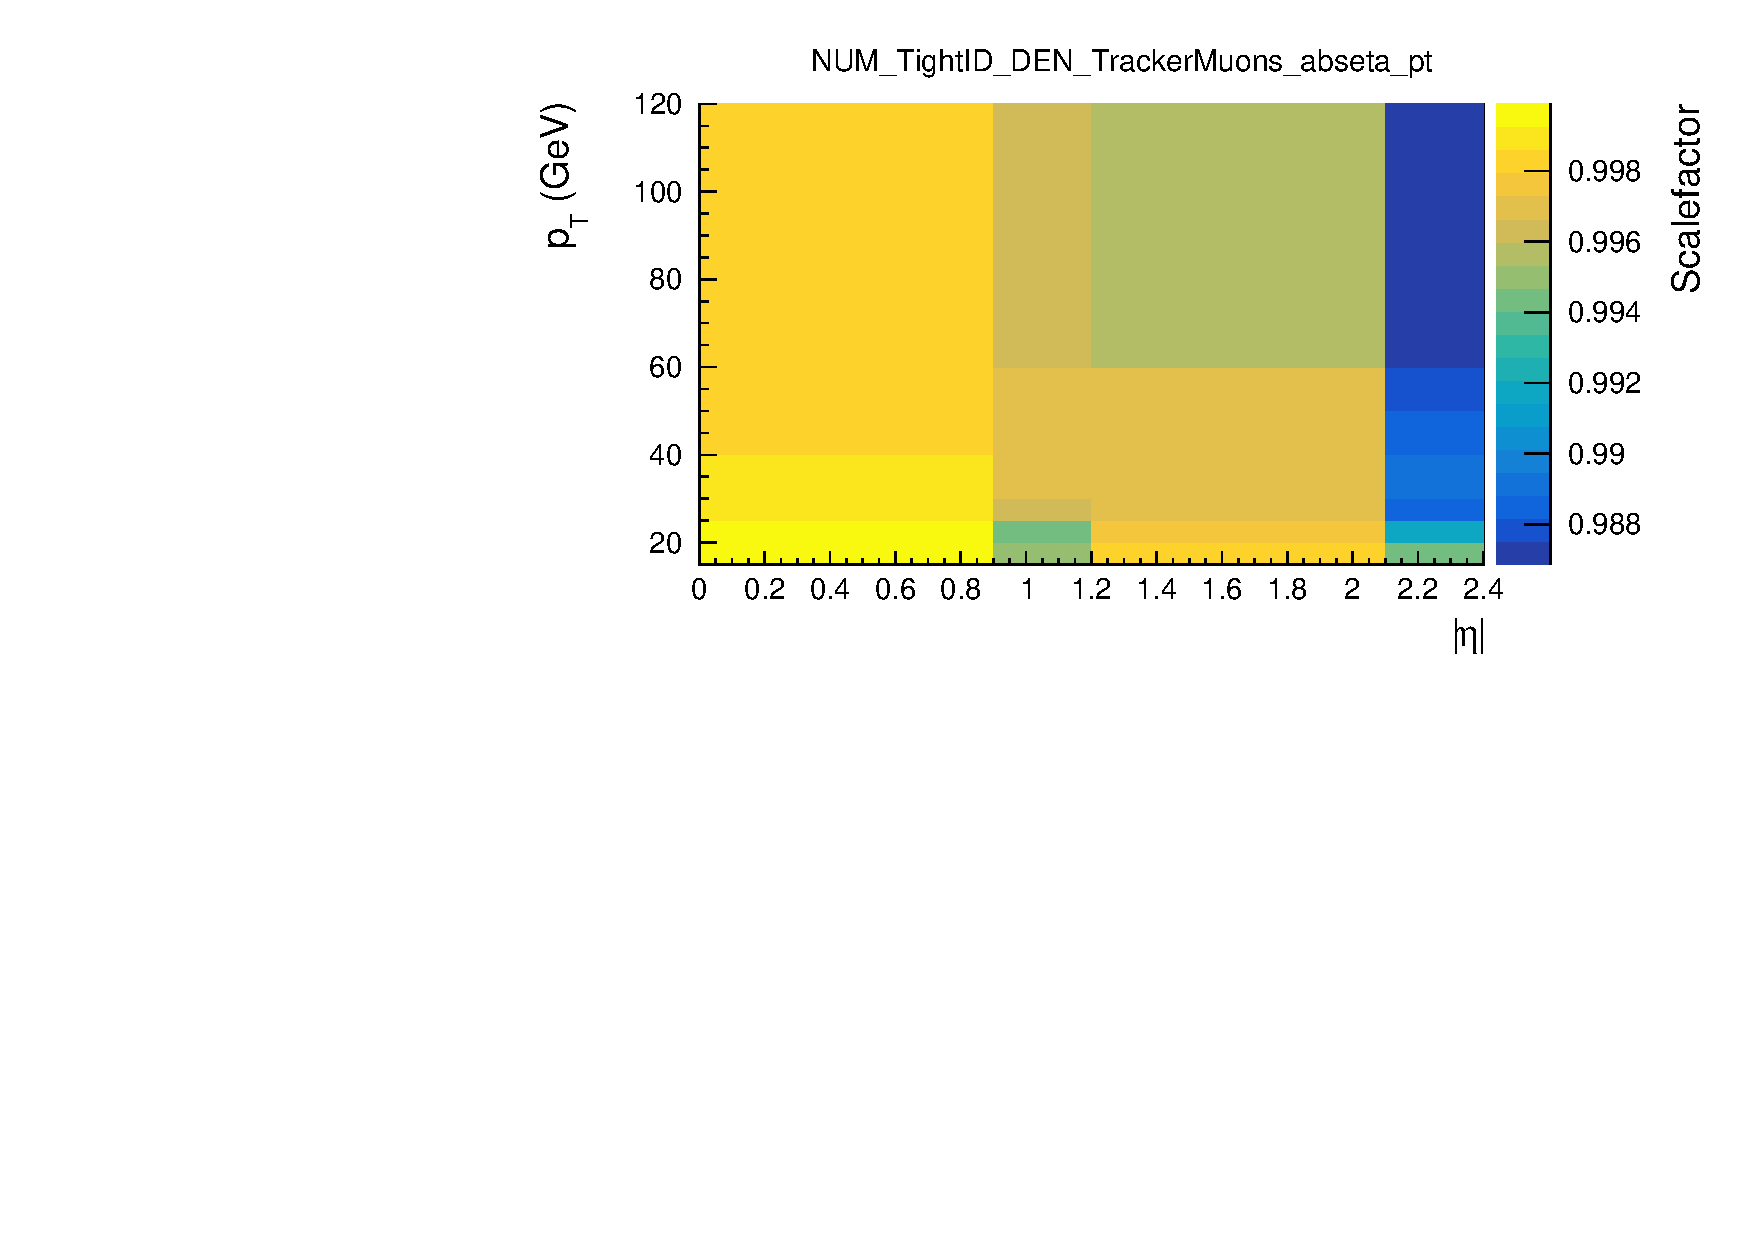
\includegraphics[height=8cm, width=10cm, trim= 0cm 0cm 0cm 0.cm,clip]{images/Muon/NUM_TightID_DEN_TrackerMuons.pdf}
    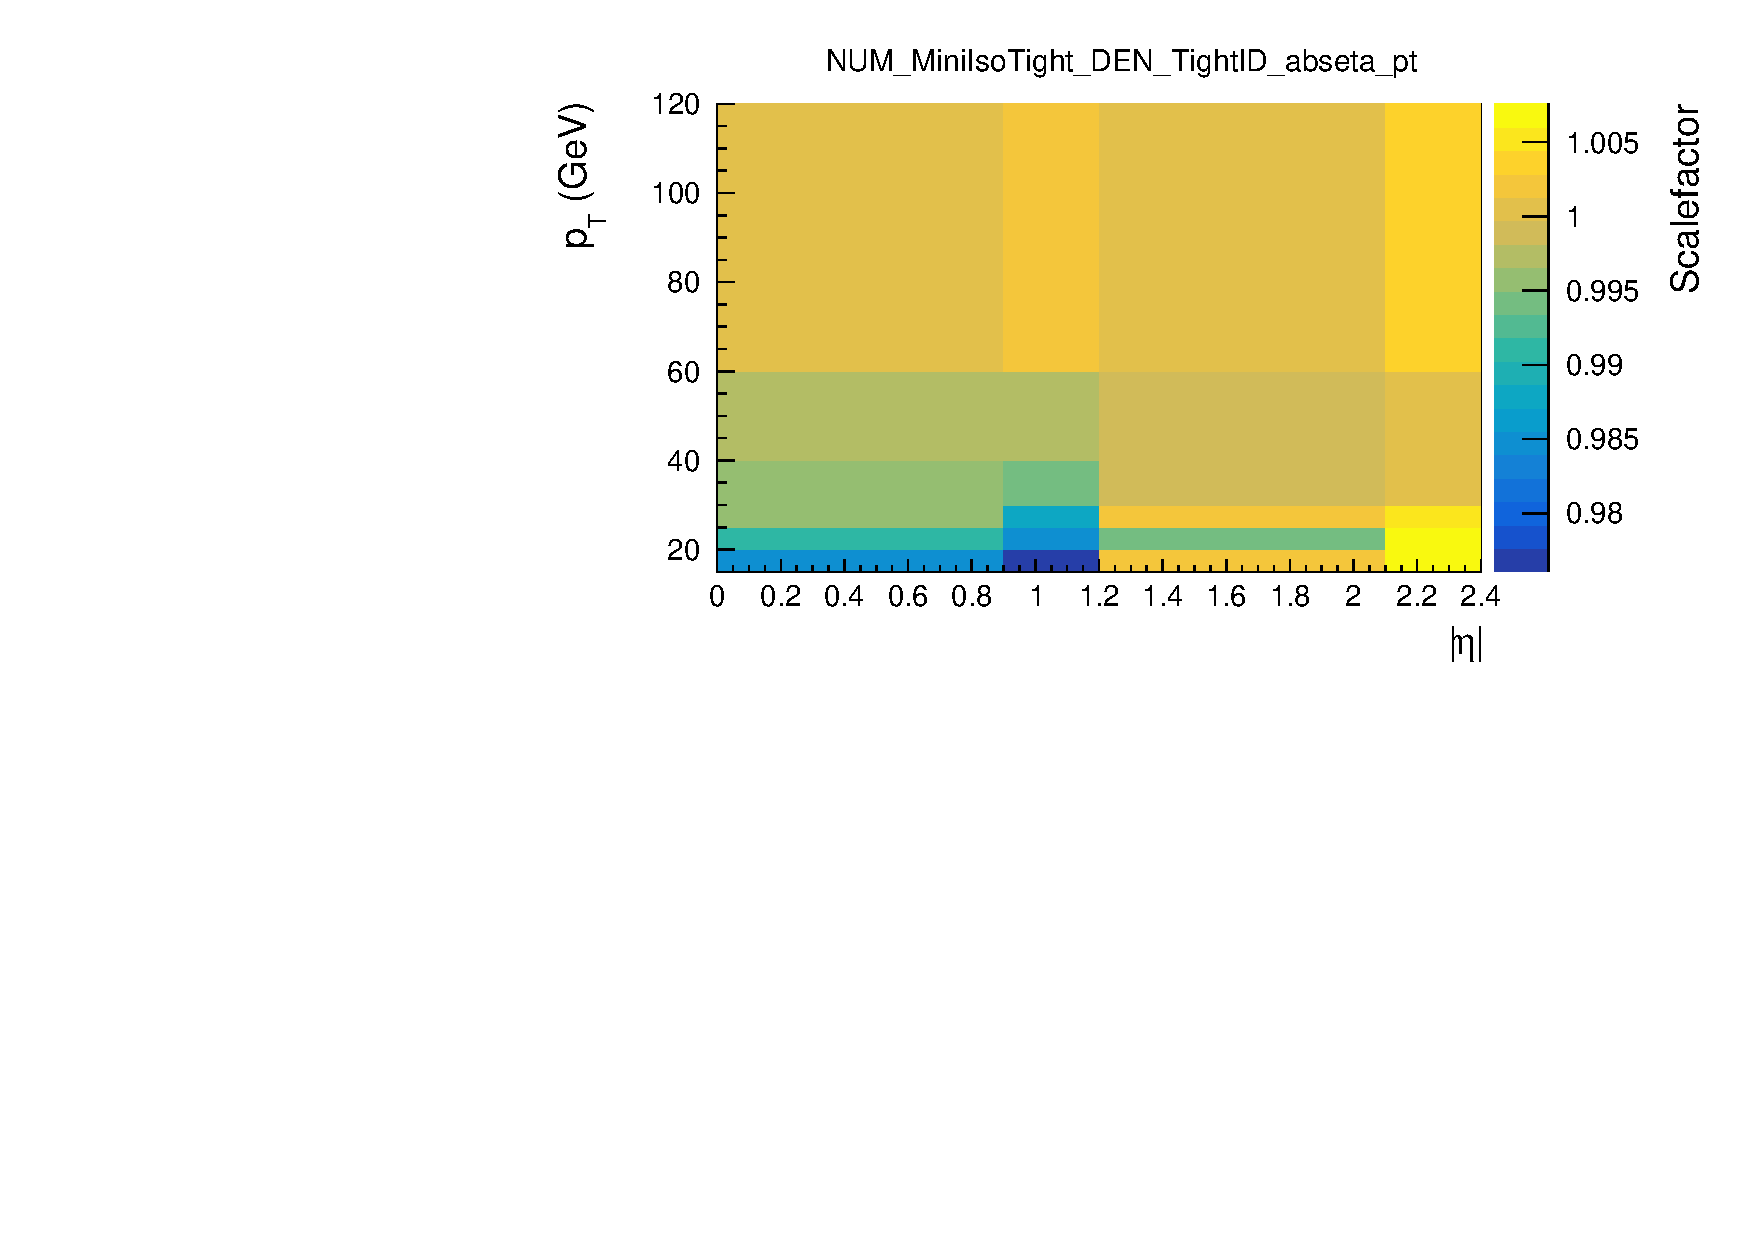
\includegraphics[height=8cm, width=10cm, trim= 0cm 0cm 0cm 0.cm,clip]{images/Muon/NUM_MiniIsoTight_DEN_TightID.pdf}
    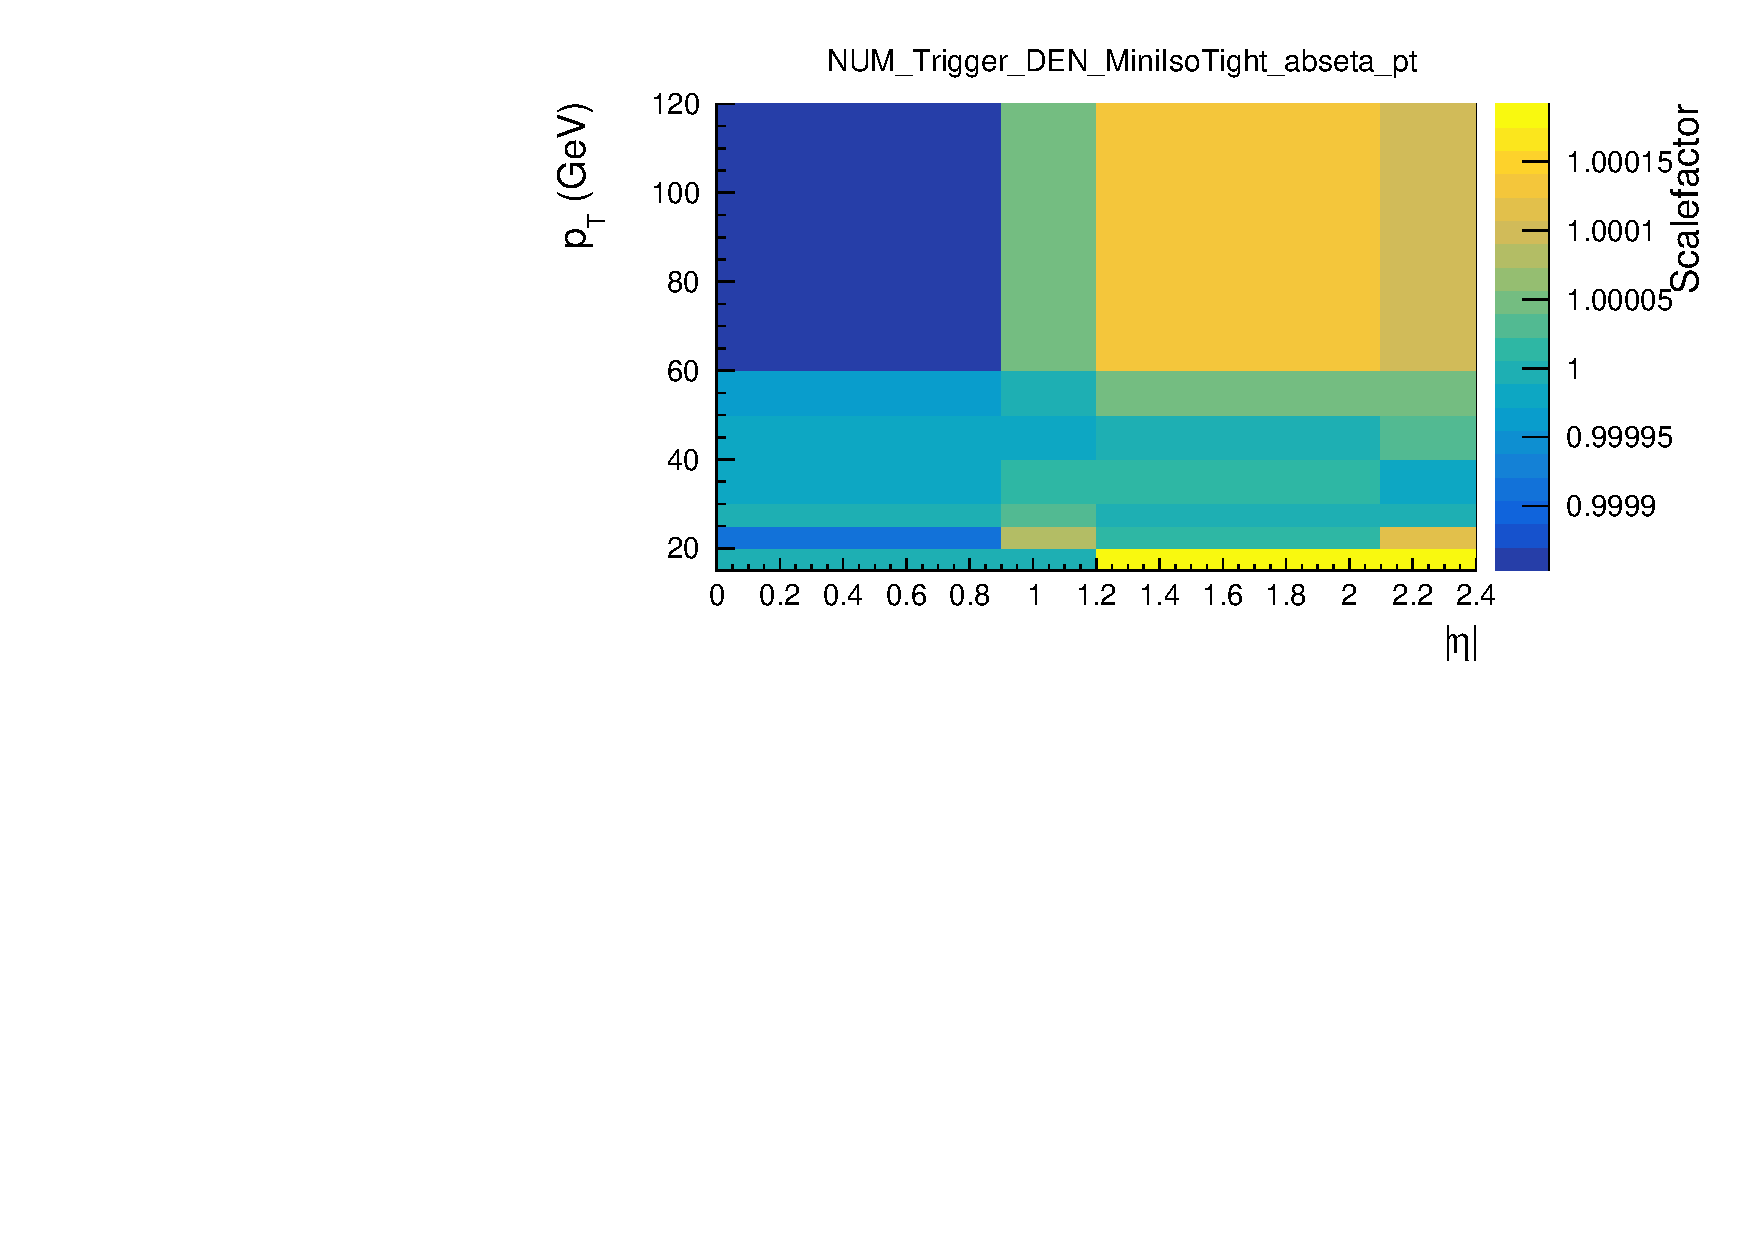
\includegraphics[height=8cm, width=10cm, trim= 0cm 0cm 0cm 0.cm,clip]{images/Muon/NUM_Trigger_DEN_MiniIsoTight.pdf}
    \caption{ Distribution of the muon scale factors in bins of $p_T$ and $\eta$. The top figure correspond to the identification SF $\epsilon^{\mu}_{ID|TRK}$, the middle figure corresponds to the isolation SF $\epsilon^{\mu}_{ISO|ID}$ and the bottom figure corresponds to the trigger SF $\epsilon^{\mu}_{Trigger|ISO}$.}
    \label{fig:SP1}
\end{figure}

    In order to match the online and offline selection of the analysis, the following selection is applied for the computation of the scale factors with Spark on the $Z\rightarrow\mu\mu$ resonance:\\
    \begin{enumerate}
        \item for 2016 : tag\_isGlobal == 1 and probe\_isGlobal == 1 and abs(probe\_dxy)$<$0.1 and abs(probe\_dz)$<$0.2 and abs(tag\_dxy)$<$0.1 and abs(tag\_dz)$<$0.2 and tag\_isTight == 1 and tag\_MiniIsoTight == 1 and tag\_pt$>$25 and probe\_pt$>$10  and abs(tag\_eta)$<$2.4 and probe\_abseta$<$2.4 and tag\_HLT\_Mu17\_TrkIsoVVL\_Mu8\_TrkIsoVVL\_v and pair\_mass $>$ 10
        
        \item for 2017 : tag\_isGlobal == 1 and probe\_isGlobal == 1 and abs(probe\_dxy)$<$0.1 and abs(probe\_dz)$<$0.2 and abs(tag\_dxy)$<$0.1 and abs(tag\_dz)$<$0.2 and tag\_isTight == 1 and tag\_MiniIsoTight == 1 and tag\_pt$>$25 and probe\_pt$>$10  and abs(tag\_eta)$<$2.4 and probe\_abseta$<$2.4 and ( tag\_HLT\_Mu17\_TrkIsoVVL\_Mu8\_TrkIsoVVL\_DZ\_Mass3p8\_v == 1 or \\ tag\_HLT\_Mu17\_TrkIsoVVL\_Mu8\_TrkIsoVVL\_DZ\_Mass8\_v ) and pair\_mass $>$ 10
        
        \item for 2018 :  tag\_isGlobal == 1 and probe\_isGlobal == 1 and abs(probe\_dxy)$<$0.1 and abs(probe\_dz)$<$0.2 and abs(tag\_dxy)$<$0.1 and abs(tag\_dz)$<$0.2 and tag\_isTight == 1 and tag\_MiniIsoTight == 1 and tag\_pt$>$25 and probe\_pt$>$10  and abs(tag\_eta)$<$2.4 and probe\_abseta$<$2.4 and tag\_HLT\_Mu17\_TrkIsoVVL\_Mu8\_TrkIsoVVL\_DZ\_Mass3p8\_v == 1  and pair\_mass $>$ 10
    \end{enumerate}

The final scale factor is defined as the combination of four efficiencies :
\begin{equation}
    SF^{\mu} = \epsilon^{\mu}_{TRK} *\epsilon^{\mu}_{ID|TRK} * \epsilon^{\mu}_{ISO|ID} * \epsilon^{\mu}_{Trigger|ISO}
\end{equation}

where :
\begin{itemize}
    \item $\epsilon^{\mu}_{TRK}$ is the tracking efficiency really close to unity and set to 1 by the MuonPOG
    \item $\epsilon^{\mu}_{ID|TRK}$ is the ratio of muons passing a given Identification flag with respect to the number of tracker muons (to follow the computation of the Muon POG)
    \item $\epsilon^{\mu}_{ISO|ID}$ is the ratio of muons passing a given Isolation flag with respect to the number of muon passing the Identification flag
    \item $\epsilon^{\mu}_{Trigger|ISO}$ is the ratio of muons passing the trigger requirement with respect to the number of muons passing the Isolation criteria (and Identification flag).
\end{itemize}
These efficiencies are computed for each necessary combination \cite{MuonSpark3} of ID/ISO/trigger of muons  indicated in the Table.\ref{tab:MUONSEL}.



    \subsection{Electrons}

    Electrons are objects that have a dedicated tracking algorithm, the Gaussian Sum Filter tracking \cite{Adam_2005} algorithm that uses the information of the tracker and the ECAL to reconstruct the track of electrons taking into account the bremsstrahlung.

    These prompt electrons in the electron-muon channel (for background estimation but also in the potential electron channel) are required to have constraints on their impact parameters, to be of opposite charge and also to follow the electronID and Isolation given in the Table.\ref{tab:ELSEL}. Electron IDs and corrections are implemented following the EGamma POG using the EGammaPostRecoTools \cite{EgammaPostRecoTools}.

    \begin{table}[h]
\centering
\begin{tabular}{|c|c|c|c|}
  \hline
  \rowcolor{lightgray} 
  Selection & $Prompt_{|\eta|<1.479}$ & $Prompt_{|\eta|> 1.556}$ & Others \\
  \hline
  $|\eta|$ & 1.479 & 2.4 & 2.4 \\
  $p_T$ & 10 & 10 & 10\\
  $|d_{dxy}|$ & 0.05 cm  & 0.10 cm & none\\
  $|d_{dz}|$ & 0.10 cm & 0.20 cm & none\\
  TightID & True & True & False\\
  \hline
\end{tabular}
    \caption{Selections for the prompt Electrons in the electron channel. The TightID refers to the "cutBasedElectronID-Fall17-94X-V2-tight" working point from the EGamma POG.}
    \label{tab:ELSEL}
\end{table}



    \subsection{Jets}
        \label{SUB:JETS}

    This analysis aims at looking at Run 2 and Run 3 data. This involves different types of jets between the two data-taking periods. For Run 2, AK4PF jets are used where AK4PF indicates the clustering of Particle-Flow candidates through the anti-$k_T$ algorithm \cite{ANTIKT} with a distance parameter of 0.4. The selection applied on jets are summarized in Table.\ref{tab:JETSEL}. Further selections will be applied on jets for the event reconstruction. The $p_T$  distribution in Fig.\ref{fig:JetPt} shows that the signal tends to be more energetic than the Standard Model $t\bar{t}$ background. The $\Delta R$   distribution in Fig.\ref{fig:JetdR} shows the tendency of the two leading jets to be more back-to-back compared to the $t\bar{t}$ background.
\begin{figure}[ht]
\centering
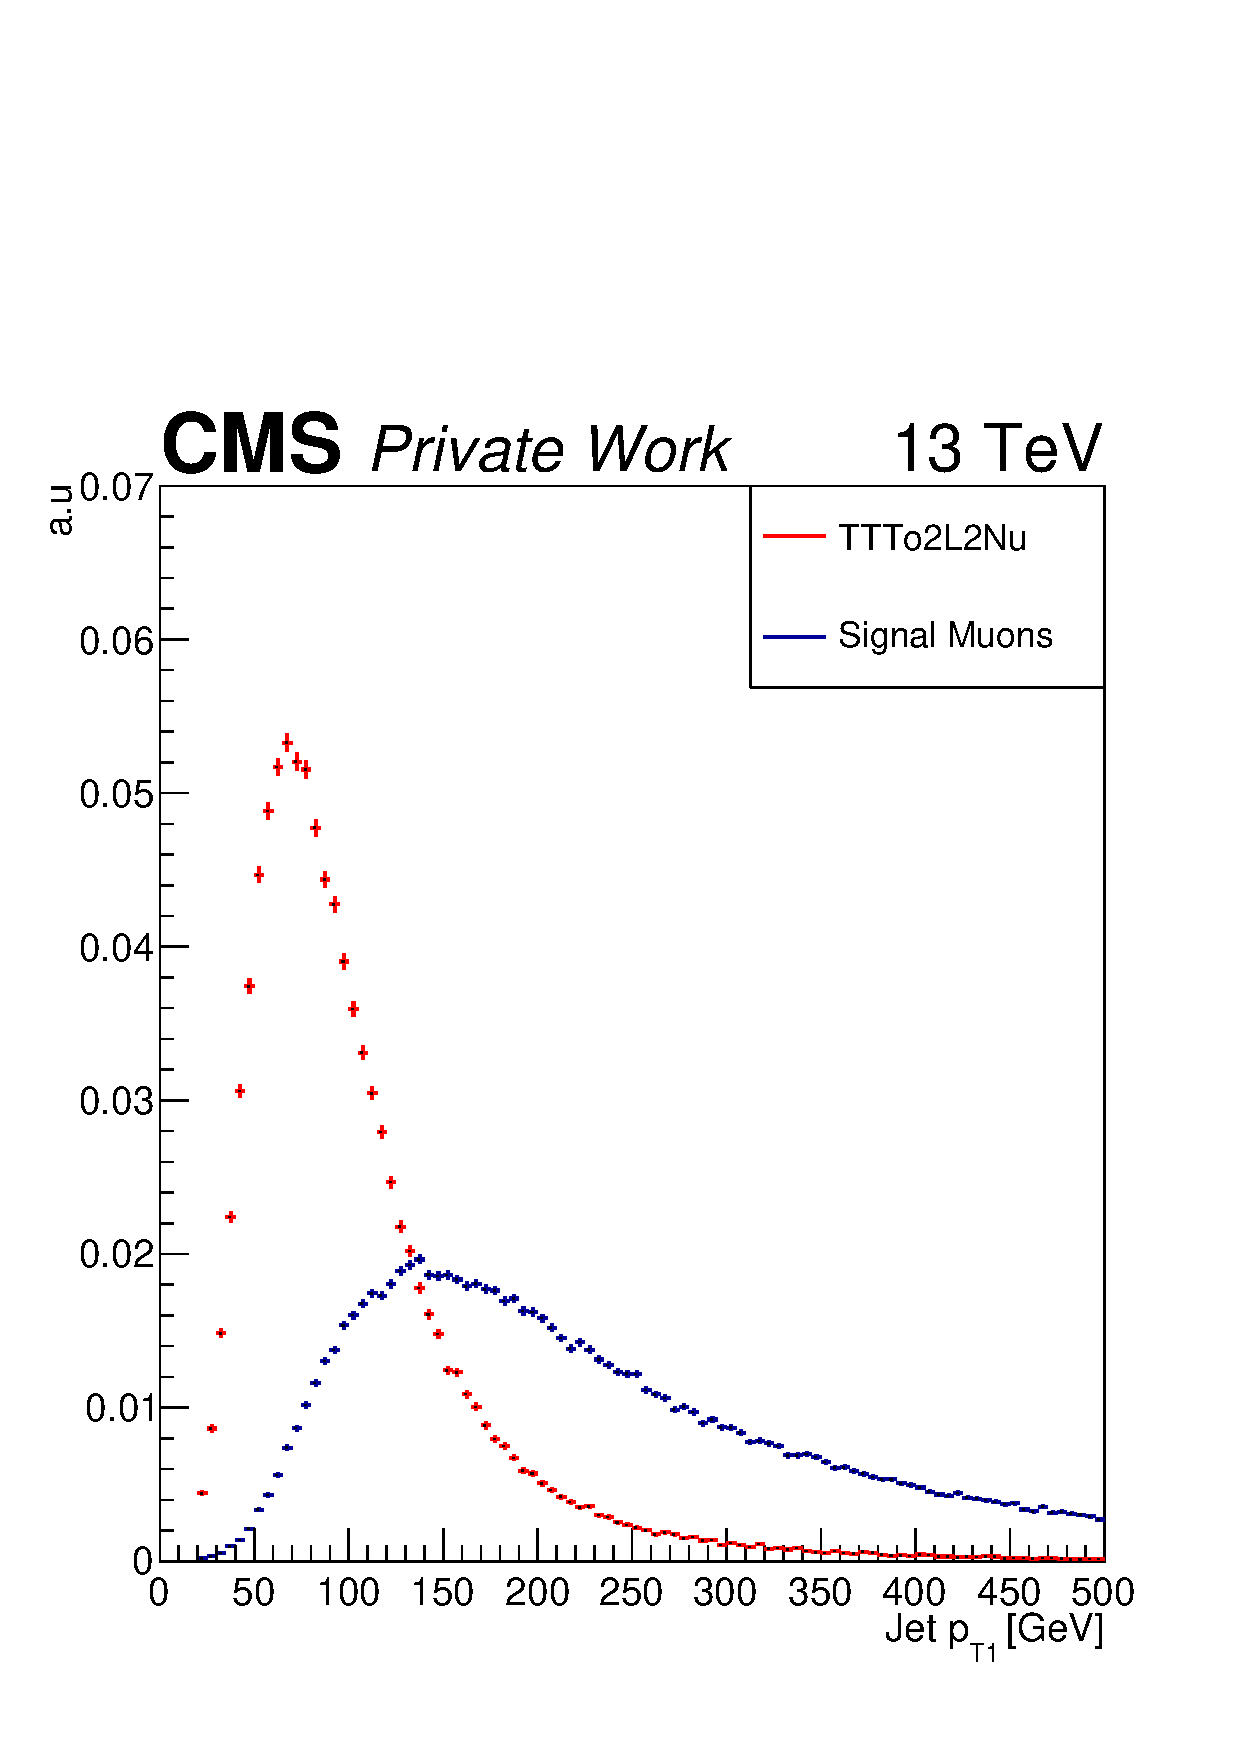
\includegraphics[height=8cm, width=8cm, trim= 0cm 0cm 0cm 0.cm,clip]{images/Jet/JetLeadingPt.pdf}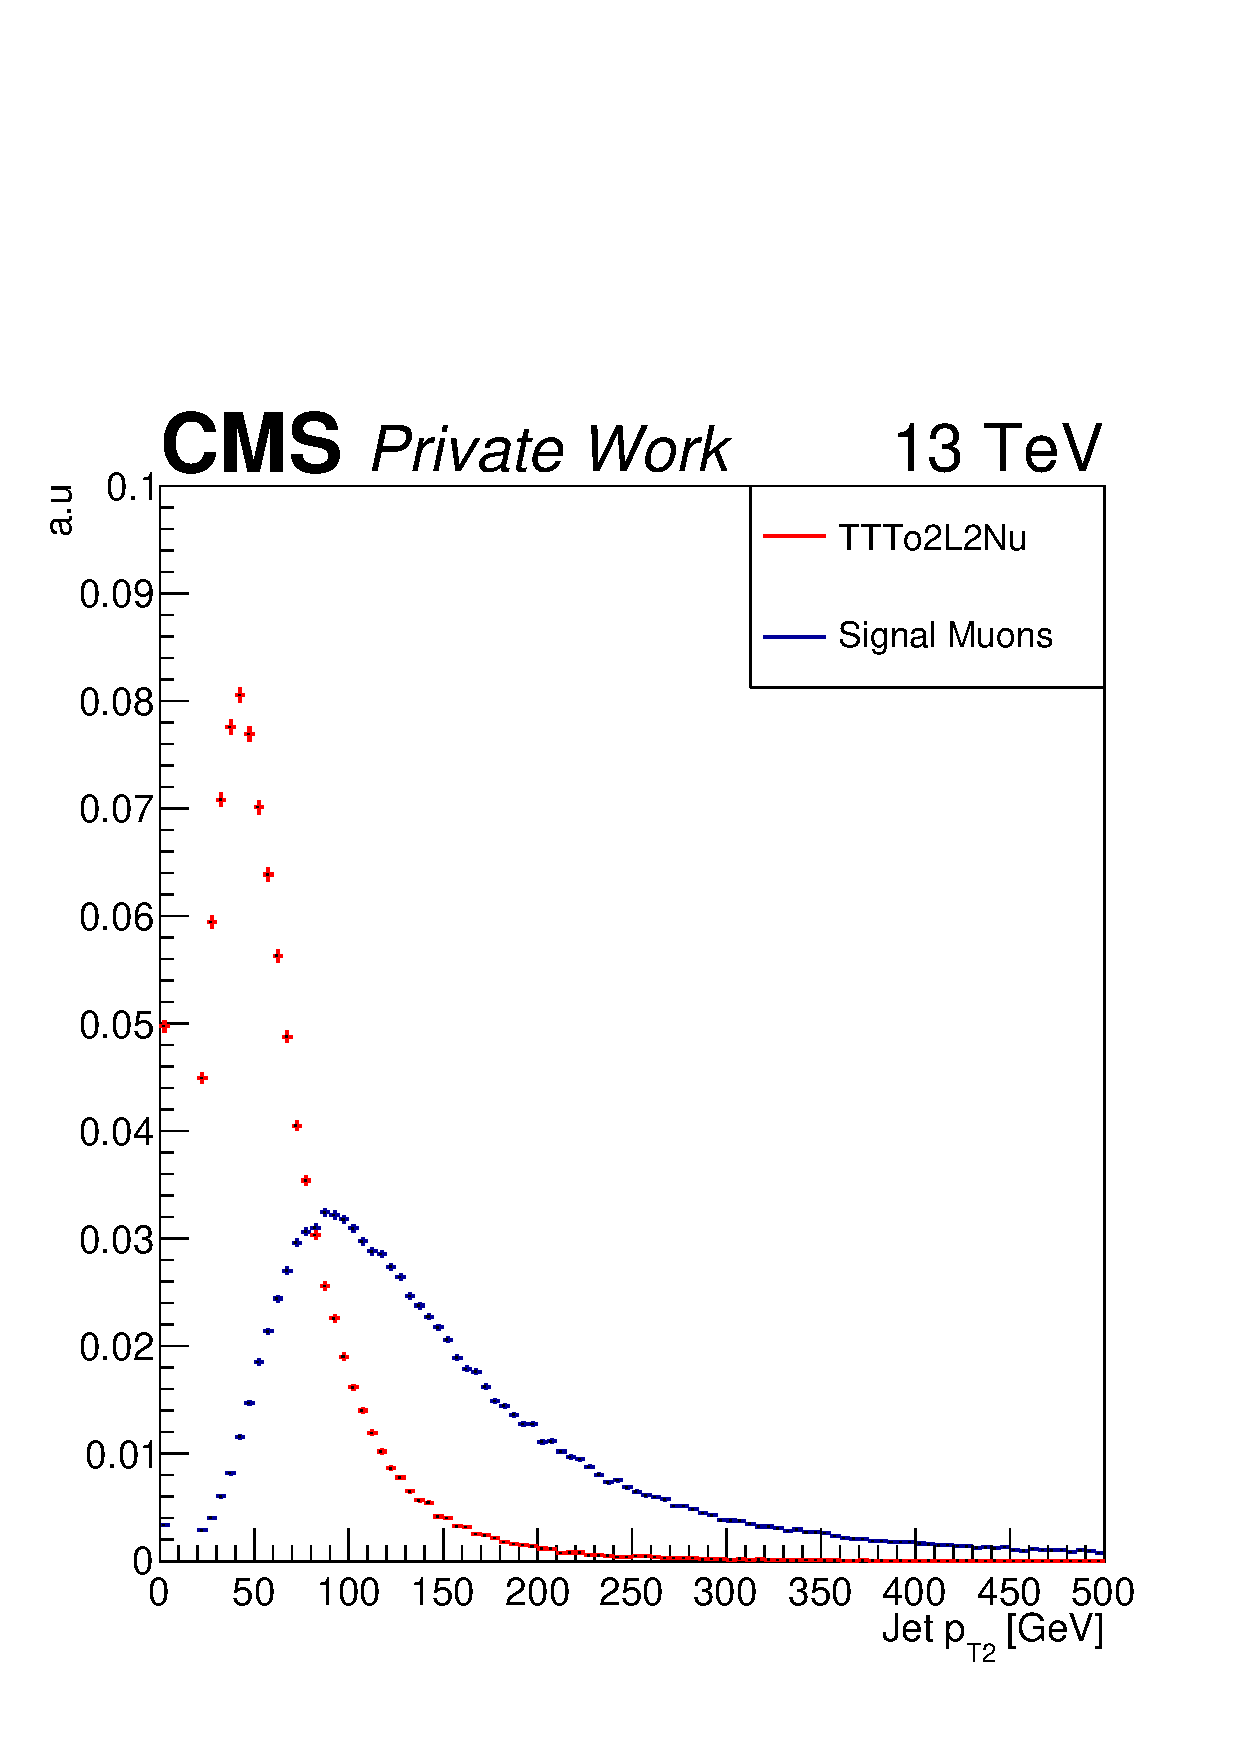
\includegraphics[height=8cm, width=8cm, trim= 0cm 0cm 0cm 0.cm,clip]{images/Jet/JetLeadingPt2.pdf}
\caption{\label{fig:JetPt} Distributions of the leading and sub-leading jet $p_T$ in signal events and $t\bar{t}$ MC events.}
\end{figure}
\FloatBarrier


\begin{figure}[ht]
\centering
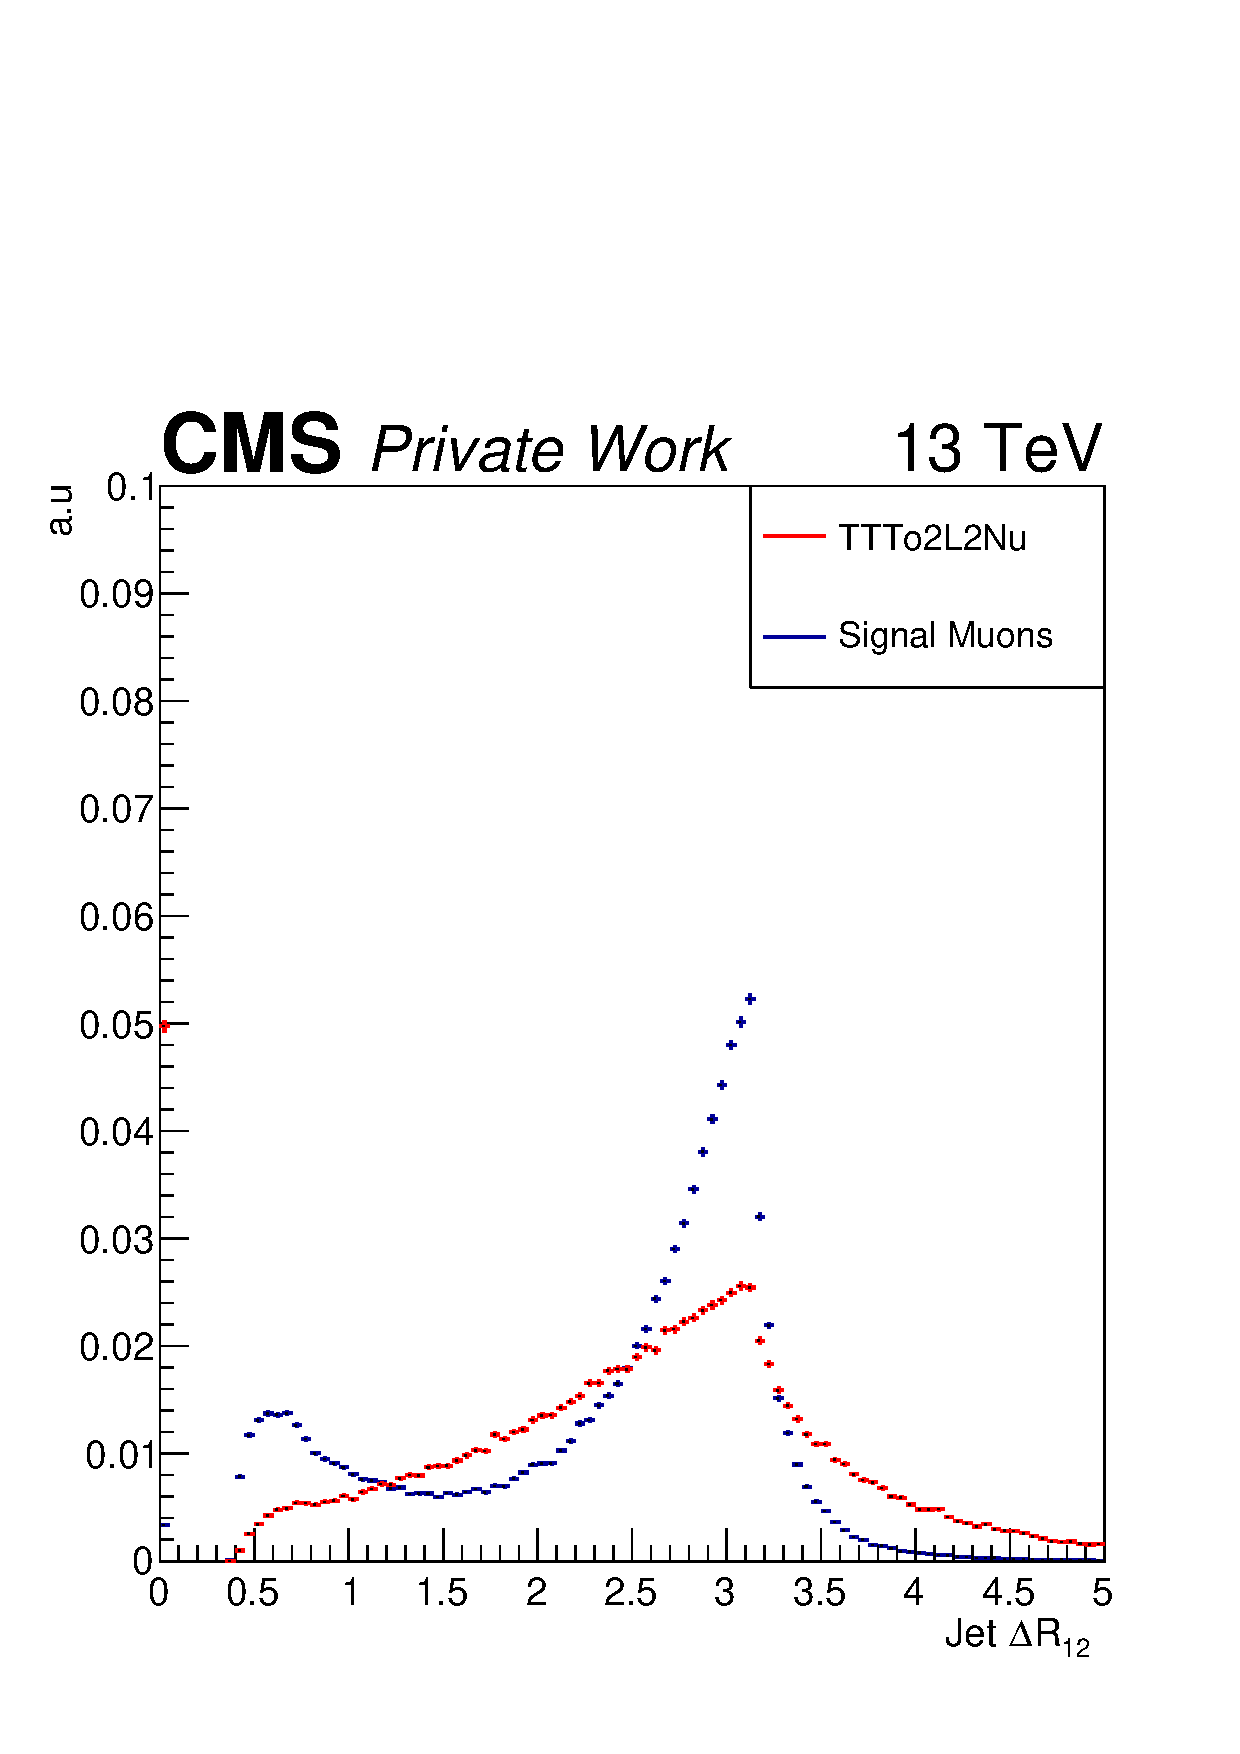
\includegraphics[height=8cm, width=8cm, trim= 0cm 0cm 0cm 0.cm,clip]{images/Jet/JetJetdR.pdf}
\caption{\label{fig:JetdR}  $\Delta R$ distribution between the leading and sub-leading jets in signal and $t\bar{t}$ MC events.}
\end{figure}
\FloatBarrier

\begin{table}[h]
\centering
\begin{tabular}{|c|c|}
  \hline
  \rowcolor{lightgray} 
  Selection & Value \\
  \hline
  $p_T$ & 20 \\
  TightLepVetoId & True \\
  \hline
\end{tabular}
    \caption{Selections for the jets with the TightID referring to the recommendation of the Jets POG\cite{TIGHTJET}.}
    \label{tab:JETSEL}
\end{table}

 As a note, one could wonder the effect of the TightJetID on displaced vertices and on the final vertex reconstruction efficiency since jets are the main constituents of this physics process. It has been checked that the TightJetID and TightJetIDLepVeto select more than 90\% and 80\% respectively of the jets and that the final reconstruction efficiency of the vertices is not affected by this selection despite the loss of jets. \\

 The PUPPI Jets collection has been tested for Run 3 but the signal reconstruction efficiency decreases by a few percent while keeping the AK4PFJets maintains the signal reconstruction efficiency at the same level. Therefore, both Run 2 and Run 3 will make use of the AK4PFJets collection.


%%%%%%%%%%%%%%%%%%%%%%%%%%%%%%%%%%%%%%%%%%%%%%%%%%%%%%%%%%%%%%%
%%%%%%%%%%%%%%%%%%%%%%%%%%%%%%%%%%%%%%%%%%%%%%%%%%%%%%%%%%%%%%%
%------------------- SECTION ----------------------------------
%%%%%%%%%%%%%%%%%%%%%%%%%%%%%%%%%%%%%%%%%%%%%%%%%%%%%%%%%%%%%%%
%%%%%%%%%%%%%%%%%%%%%%%%%%%%%%%%%%%%%%%%%%%%%%%%%%%%%%%%%%%%%%%
\newpage
\section{Event Selection}
\label{SEC: EVTSEL}
    This analysis can take advantage of the two prompt leptons to select the events. One lepton is always selected by the online trigger selection and the second lepton can come from the dilepton trigger mentioned in Table.\ref{tab:TRIGGER2018} or it can also be selected offline following a specific selection on the invariant mass of the two leptons selected, detailed below. The $\tau$ channel is not studied since its decay can significantly change the experimental signature as jets from the $\tau$ decay could overlap with the displaced jets and potentially in due a bias in the reconstruction of the event detailed in section.\ref{SEC: EVTREC}. In this analysis, the two prompt leptons must be of opposite charge since the smuon is considered to be of Dirac nature.
    Adding to the selections introduced on prompt leptons in the previous section and the trigger mentioned in section.\ref{SEC: DATASET}, the first selected muon is required to have a $p_T > 25$ GeV and the second muon selected is required to have a $p_T > 10$ GeV. The invariant mass of the two selected muons is required to be above 10 GeV in order to reduce the amount of low-mass resonances in the search. 

    The topology of the event depends on the point in the phase space of the signal that is chosen where the signal can be very displaced (dozens of centimeters down to a millimeter) and also the mass spectra can change the kinematic of the event considering the signal samples mentioned in Table.\ref{tab:TAB1}.\\
    One important feature of the signal is the $t\Bar{t}$-like experimental signature where two b-jets are produced in the event. B-tagging is applied on slightly displaced vertices \cite{CMS-DP-2018-058} depending on the decay length of the B-Hadron. Since the signal event is close to a $t\bar{t}$ event, the b-tagging could have the same efficiency for both signal and background.
    Therefore, B-Tagging is not a variable that is used in this analysis since its efficiency depends on the point in the phase space we want to look for.\\

    

%     This first online+offline selection allows to reduce backgrounds up to 90\% but it is not enough in order to observe the signal in any part of the phase space. Therefore, a step further is implemented in order to reduce the background at event level using the topology of the event.

%     A multivariate analysis selection based on a Boosted Decision Tree (BDT) from the Toolkit for Multivariate Analysis (TMVA) \cite{TMVA} is implemented. The list of variables given as an input is given in Table \ref{tab:EVTBDTVAR}. The distribution of the input variables between signal and backgrounds are given in the Appendix.\ref{APP: EVTBDT}. 

% \begin{table}[h]
% \centering
% \begin{tabular}{|c|m{10 cm}|}
%   \hline
%   \rowcolor{lightgray} 
%   Variable & Definition \\
%   \hline
%   MET & Total Missing Transverse Energy \\
%   \hline
%   $H_T$ & Sum of the $p_T$ of the jets that passed through the selections in Table.\ref{tab:JETSEL}\\
%   \hline
%   $S_T$ & Sum of the $p_T$ of the muons that passed through the selections  for \textbf{Prompt} muons in Table.\ref{tab:MUONSEL}  \\
%   \hline
%   nJets & Total number of jets that have passed the selections in Table.\ref{tab:JETSEL} \\
%   \hline
%   nPromptMuons &  Total number of prompt muons that have passed the selections for \textbf{Prompt} muons in Table.\ref{tab:MUONSEL} \\
%   \hline
%   nAllMuons & Total number of muons that have passed the selections for \textbf{other} muons in Table.\ref{tab:MUONSEL} \\
%   % \hline
%   % $M_{\mu\mu}$ & Invariant mass of the two selected prompt muons from Section\ref{SEC: EVTSEL} [add table?]\\
%   \hline
%   NTracks & Total number of tracks in the event \\
%   % \hline
%   % $p_{T_{l1}}$ & Muon leading $p_T$ \\
%   % \hline
%   % $p_{T_{l2}}$ & Muon sub-leading $p_T$ \\
%   \hline
%   $p_{T_{j1}}$ & Jet leading $p_T$ \\
%   \hline
%   $p_{T_{j2}}$ & Jet sub-leading $p_T$ \\
%     \hline
%   $p_{T_{j1}}$ & Jet leading $\eta$ \\
%   \hline
%   $p_{T_{j2}}$ & Jet sub-leading $\eta$ \\
%   % \hline
%   % $\Delta R_{l_1-l_2}$ & $\Delta R$ between the leading  and sub-leading muons \\
%   % \hline
%   % $\Delta \phi_{l_1-l_2}$ & $\Delta \phi$ between the leading  and sub-leading muons \\
%   % \hline
%   %  $\Delta \eta_{l_1-l_2}$ & $\Delta \eta$ between the leading  and sub-leading muons \\
%    \hline
%   $\Delta R_{j_1-j_2}$ & $\Delta R$ between the leading  and sub-leading jets \\
%   \hline
%   $\Delta \phi_{j_1-j_2}$ & $\Delta \phi$ between the leading  and sub-leading jets \\
%   \hline
%    $\Delta \eta_{j_1-j_2}$ & $\Delta \eta$ between the leading  and sub-leading jets \\
%    \hline
%   % $\Delta R_{l_1-j_1}$ & $\Delta R$ between the leading muon and leading jet \\
%   % \hline
%   % $\Delta R_{l_1-j_2}$ & $\Delta R$ between the leading muon and sub-leading jet \\
%   % \hline
%   % $\Delta R_{l_2-j_1}$ & $\Delta R$ between the sub-leading muon and leading jet \\
%   % \hline
%   % $\Delta R_{l_2-j_2}$ & $\Delta R$ between the sub-leading muon and sub-leading jet \\
%   \hline
%   Hemi1 njet nomu & Number of jets from the first hemisphere having a $\Delta R$ above 0.4 with respect to the two prompt leptons \\
%     \hline
%   Hemi1 $p_T$ &  $p_T$ of the first reconstructed hemisphere\\
%   \hline
%   Hemi1 eta &  $\eta$ of the first reconstructed hemisphere\\
%   \hline
%   Hemi1 phi & $\phi$ of the first reconstructed hemisphere\\
%   \hline 
%   Hemi1 nTrks & (to be removed) number of tracks of the first reconstructed hemisphere\\
%   \hline
%   Hemi2 njet nomu & Number of jets from the second hemisphere having a $\Delta R$ above 0.4 with respect to the two prompt leptons\\
%   \hline
%   Hemi2 pt & $p_T$ of the second reconstructed hemisphere\\
%   \hline
%   Hemi2 eta & $\eta$ of the second reconstructed hemisphere\\
%   \hline
%   Hemi2 phi & $\phi$ of the second reconstructed hemisphere\\
%   \hline
%   Hemi2 nTrks & (to be removed) number of tracks of the second reconstructed hemisphere\\
%   \hline
%   Mass of Hemisphere 1 & Mass of the first reconstructed hemisphere using the jets \\
%   \hline
%   Mass of Hemisphere 2 & Mass of the second reconstructed hemisphere using the jets \\
%   \hline

% \end{tabular}
%     \caption{Input variables for the Event selection BDT}
%     \label{tab:EVTBDTVAR}
% \end{table}
% \FloatBarrier


    
%     [ADD all infos about the EVT BDT SEL OR CUT]

%     \subsubsection{Dependence of the Event selection BDT with respect to the phase space}
%     will be written when we will agree on the ABCD method since the evt BDT might not be useful

%%%%%%%%%%%%%%%%%%%%%%%%%%%%%%%%%%%%%%%%%%%%%%%%%%%%%%%%%%%%%%%
%%%%%%%%%%%%%%%%%%%%%%%%%%%%%%%%%%%%%%%%%%%%%%%%%%%%%%%%%%%%%%%
%------------------- SECTION ----------------------------------
%%%%%%%%%%%%%%%%%%%%%%%%%%%%%%%%%%%%%%%%%%%%%%%%%%%%%%%%%%%%%%%
%%%%%%%%%%%%%%%%%%%%%%%%%%%%%%%%%%%%%%%%%%%%%%%%%%%%%%%%%%%%%%%
\newpage
\section{Event Reconstruction}
\label{SEC: EVTREC}
\subsection{Hemisphere contruction}
  The final state of the neutralino signal being heavily hadronic, the event reconstruction is based on the jets from the decay of the neutralino. These jets can come from the coupling between the stop and the down and strange quarks as well as the SM decay of the top. No particular restriction is applied on the decay of the W boson from the top, both leptonic and hadronic decays are considered in this analysis and leptons originating from the W or heavy-hadron flavour decays are also considered in the event reconstruction. The event topology and kinematics depends on the phase space of the signal studied: the smuon and neutralino masses, as well as the lifetime of the neutralino.\\

  In the signal, neutralinos are pair-produced from the decay of the smuons, and decay further away in the tracker. Both neutralinos tend to be back-to-back in azimuth ($\phi$) but close in $\eta$, see Fig.\ref{fig:dRNEUNEU} and Fig.\ref{fig:Geometry}, meaning that there are two clusters of tracks, mainly coming from jets, back-to-back in $\phi$. The 3D-space is then divided into two hemispheres, one for each neutralino. A precaution is applied as the prompt muons can overlap with the displaced jets, so the momentum-vector of the prompt leptons are discarded in this building procedure to avoid any bias, then jets are re-ordered by decreasing value of $p_T$. The hemispheres are defined as follows : 
    \begin{itemize}
        \item From the collections of jets ordered by decreasing value of $p_T$, the first jet is taken as the first axis of a first hemisphere
        \item Then, by looking at the other jets, if the $\Delta R$ between the jet and the first axis is below 1.5, we add the momentum-vectors of the two jets to correct on the first axis, else we build a second axis.
        \item  Finally, we iterate over all the jets and assign them to one among both hemispheres and recompute the hemisphere momentum vector for each new jet
        \item If any jets is not involved in this procedure, it is discarded from the analysis
    \end{itemize}


The goal of the analysis is to reconstruct one vertex per hemisphere.

\begin{figure}[ht]
\centering
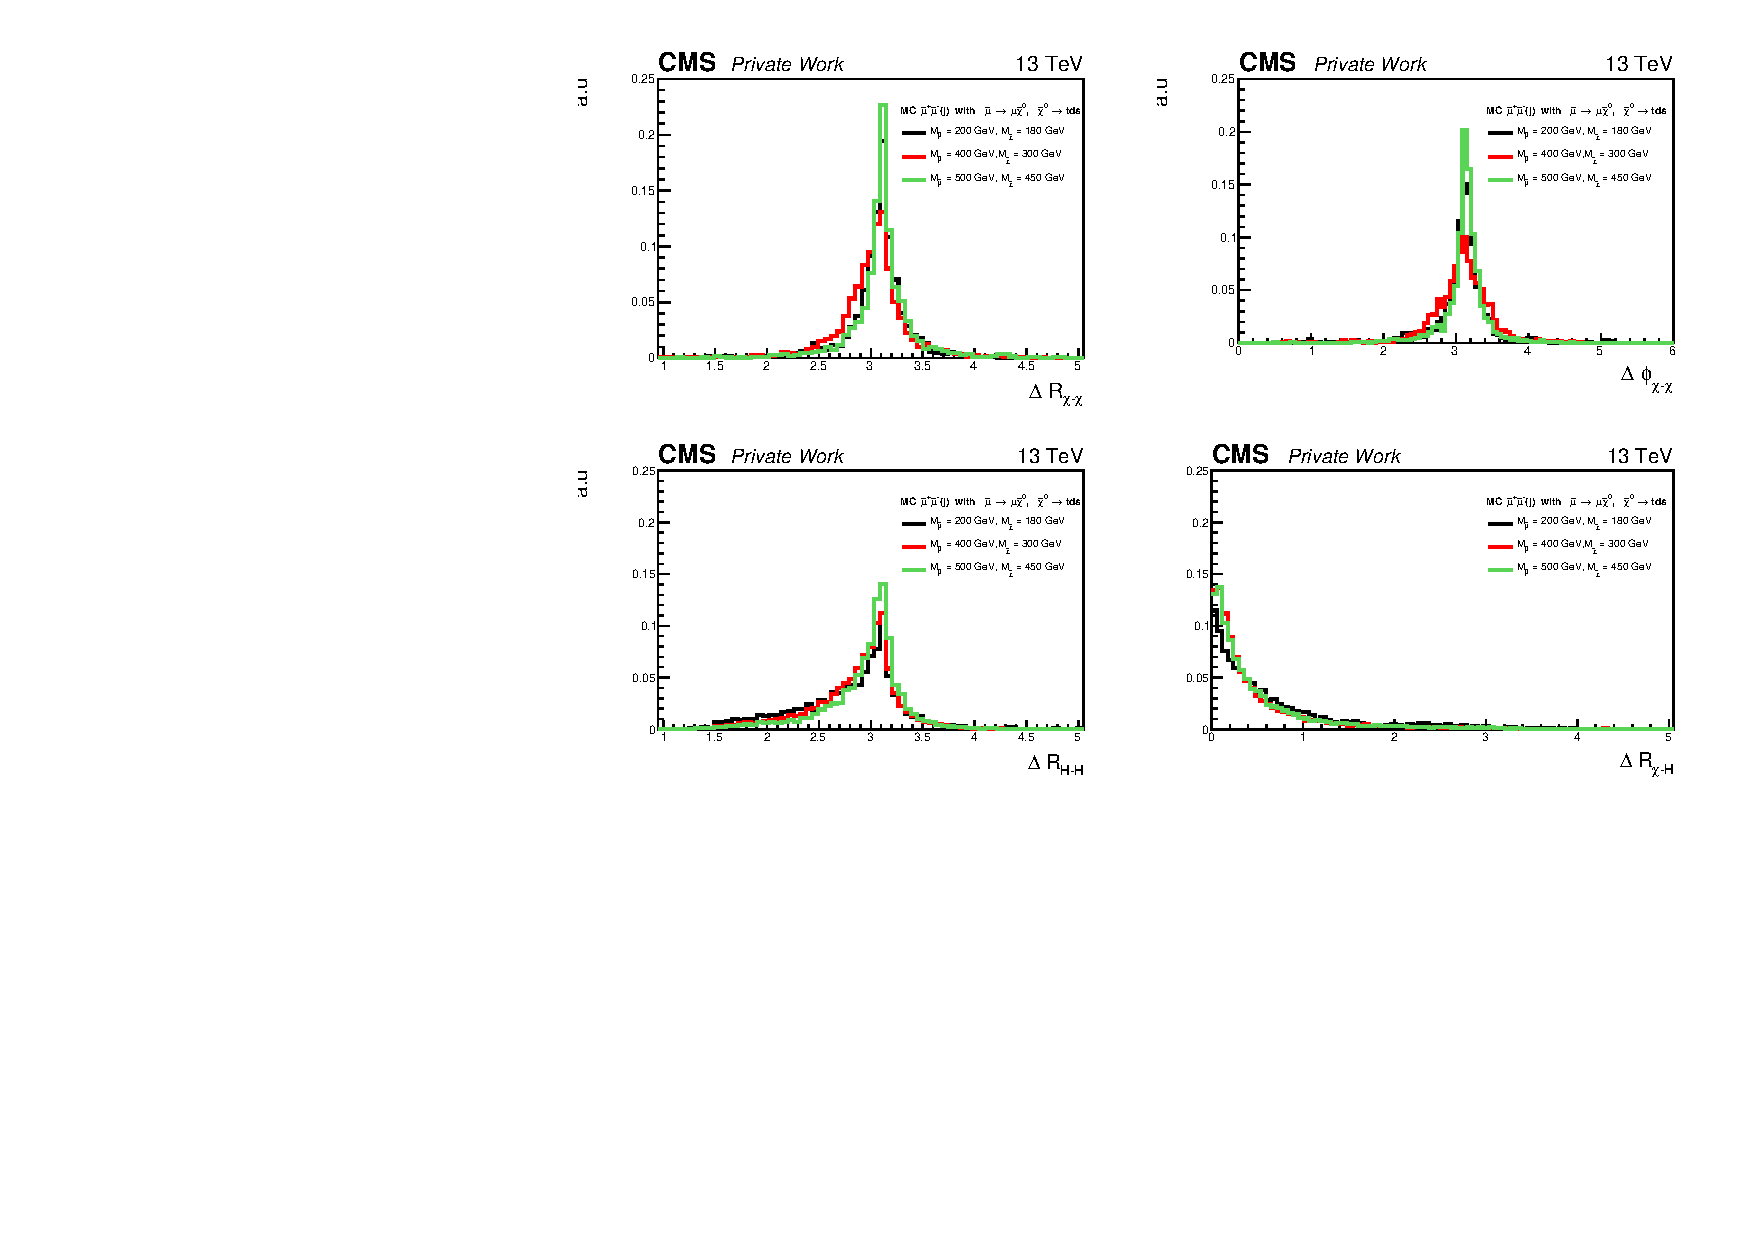
\includegraphics[height=14cm, width=17cm, trim= 2cm 0cm 0cm 0.cm,clip]{images/Topology/dPhi_GenGen.pdf}
\caption{\label{fig:dRNEUNEU} Top Left : $\Delta R$ between the two generated neutralinos. Top Right :  $\Delta \phi$ between the two generated neutralinos. Bottom Left : $\Delta R$ between the two reconstructed hemispheres. Bottom Right : $\Delta R$ between the generated neutralino and reconstructed hemisphere. The last plot shows a quite long tail indicating a mis-reconstruction of the axis in some cases, potentially when the neutralino decays outside of the tracker (or close to the end of the tracker) or an overlap between the two hemispheres.}
\end{figure}

\begin{figure}[ht]
\centering
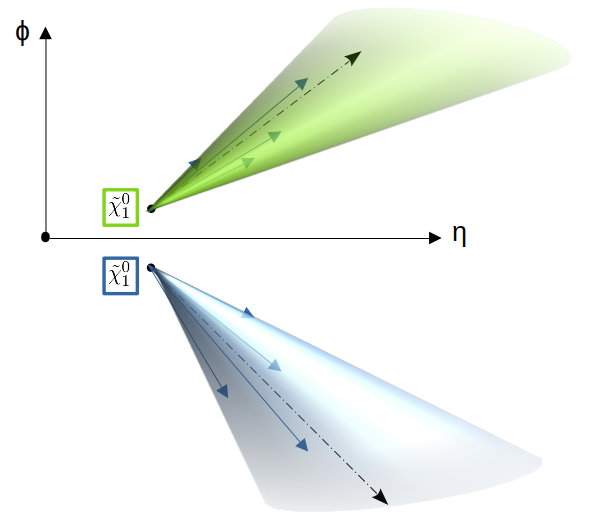
\includegraphics[height=6cm, width=8cm, trim= 0cm 0cm 0cm 0.cm,clip]{images/Topology/topo.png}
\caption{\label{fig:Geometry} Schematic view of the decay of the two neutralinos}
\end{figure}
\FloatBarrier

\subsection{Quality of the reconstructed axes}

    The quality of the reconstructed axes can be estimated by comparing the generated axis of the neutralino and the axis of the reconstructed hemisphere associated. The axis reconstruction depends on the number of jets available, their ordering (by decreasing value of $p_t$) and also the $\Delta R$ criteria that is imposed for the jets to axis association ($\Delta R <$1.5).
    The $\Delta R$ distribution between the reconstructed axis of the hemisphere and the generated neutralino is given in Fig. \ref{fig:AXESQUALITY} as a function of the neutralino mass, smuon mass and neutralino $c\tau$. About 10\% of the hemispheres are not well reconstructed. This can happen for many reasons: the decay length of the neutralino is very high reaching the end of the tracker volume, hence leaving not many jets in the tracker. It can also happened that there is a mis-association of the jets between the two hemispheres if the two neutralinos are closer than $\Delta R $ = 3, therefore inducing a bias in the hemisphere building procedure. The plot on the right indicates that for higher $\Delta M_{\Tilde{\mu}-\Tilde{\chi}^{1}_{0}} = M_{\Tilde{\mu}} - M_{\Tilde{\chi}^{1}_{0}}$, the hemisphere reconstruction efficiency is slightly lower, still reaching 85\%, while for lower $\Delta M_{\Tilde{\mu}-\Tilde{\chi}^{1}_{0}}$, this efficiency reaches 95\%. In the former case where the $\Delta M_{\Tilde{\mu}-\Tilde{\chi}^{1}_{0}}$ is lower, jets from the decay of the neutralino are less energetic, hence not passing the selections inducing a lack of information to complete the building procedure. Finally, the top from the neutralino can be produced at large angles with respect to the neutralino, therefore, the jets from the top are still used for the building procedure but are pointing towards the top direction and not the neutralino one. All these effects can explain why the hemisphere building procedure is not reaching 100\% even though the efficiency remains high.
\begin{figure}[ht]
\centering
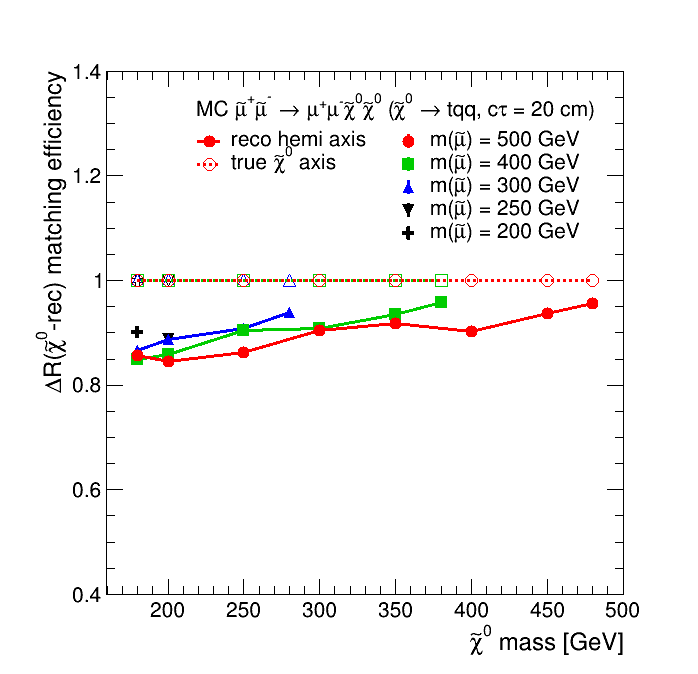
\includegraphics[height=10cm, width=10cm, trim= 0cm 0cm 0cm 0.cm,clip]{images/Topology/eff_dR_trueaxis.png}
\caption{\label{fig:AXESQUALITY} $\Delta R$ between the generated neutralino and the reconstructed axis as a function of the neutralino and smuon masses for a given $c\tau$ of 20 cm.}
\end{figure}


\FloatBarrier
%%%%%%%%%%%%%%%%%%%%%%%%%%%%%%%%%%%%%%%%%%%%%%%%%%%%%%%%%%%%%%%
%%%%%%%%%%%%%%%%%%%%%%%%%%%%%%%%%%%%%%%%%%%%%%%%%%%%%%%%%%%%%%%
%------------------- SECTION ----------------------------------
%%%%%%%%%%%%%%%%%%%%%%%%%%%%%%%%%%%%%%%%%%%%%%%%%%%%%%%%%%%%%%%
%%%%%%%%%%%%%%%%%%%%%%%%%%%%%%%%%%%%%%%%%%%%%%%%%%%%%%%%%%%%%%%
\newpage
\section{Selection of displaced Tracks}
\label{SEC: DISTRK}
    This analysis aims at reconstructing displaced vertices from the decay of a neutral long-lived particle. An important part of this analysis is devoted to the selection of displaced tracks coming from the decay of the neutralino. The displacement is dependant on the signal sample that we want to look for, therefore the selections are  applied as independently as possible from the decay length of the neutralino.\\

    The background coming from the SM is mostly prompt backgrounds with prompt tracks associated to them but secondary displaced vertices can be observed due to different sources such as $V^0$ candidates, photon conversions and other nuclear interactions within the material budget of the tracker of CMS.

    In this analysis, we are aiming to first reduce the amount of tracks coming from these backgrounds (after the event selection mentioned in section.\ref{SEC: EVTSEL}) and then select the displaced tracks. In the CMS Software (CMSSW), there are already collections containing the $V^0$ candidates and the photon conversions. These collections will not be directly used for selections but to control the selections that are applied below.

    
    \subsection{Tracks from $V^0$ candidates}
        $V^0$ candidates stands for two hadrons : the $K^0_S$ meson and the $\Lambda^{0}$ baryon. These hadrons are produced from the hadronization of the strange quark. They have a long lifetime (about $10^{-10}$ s) and produce  displaced vertices with a lower track multiplicity (2-tracks vertices) compared to signal vertices (between 6 and 10 jets). Therefore, these vertices can be identified and the tracks associated to these vertices can be removed from the workflow and not be used later.
         As stated above, CMSSW already gives a collection of the $V^0$ candidates \cite{V0CAND} but there are not directly used. Using a copy of the CMSSW code to built the $V^0$ candidates and changing it to MiniAOD, see Appendix.\ref{APP: COVMAT} and \ref{APP: FIRSTHIT}, we reconstruct the  $V^0$ candidates using the Kalman Filter \cite{KVF} by looking at any pair of tracks of opposite signs, potentially signal tracks.\\
        If all the conditions from CMSSW are passed and a $V^0$ candidate is built, the tracks associated to this candidate are removed from the analysis considering a tighter selection in mass compared to the CMSSW collection, see Fig.\ref{fig:V0Candidates}.\\

        The monitoring of this method is done by comparing between data and MC, the collection that we build in the workflow, see Fig.\ref{fig:K0DATAMC} and \ref{fig:L0DATAMC}. From the collection of reconstructed $V^0$ candidates (not the one of CMSSW), we get 1.1 $V^0$ candidates per signal and $t\Bar{t}$ event.

        
\begin{figure}[ht]
%\centering
\hspace{-1.4cm}
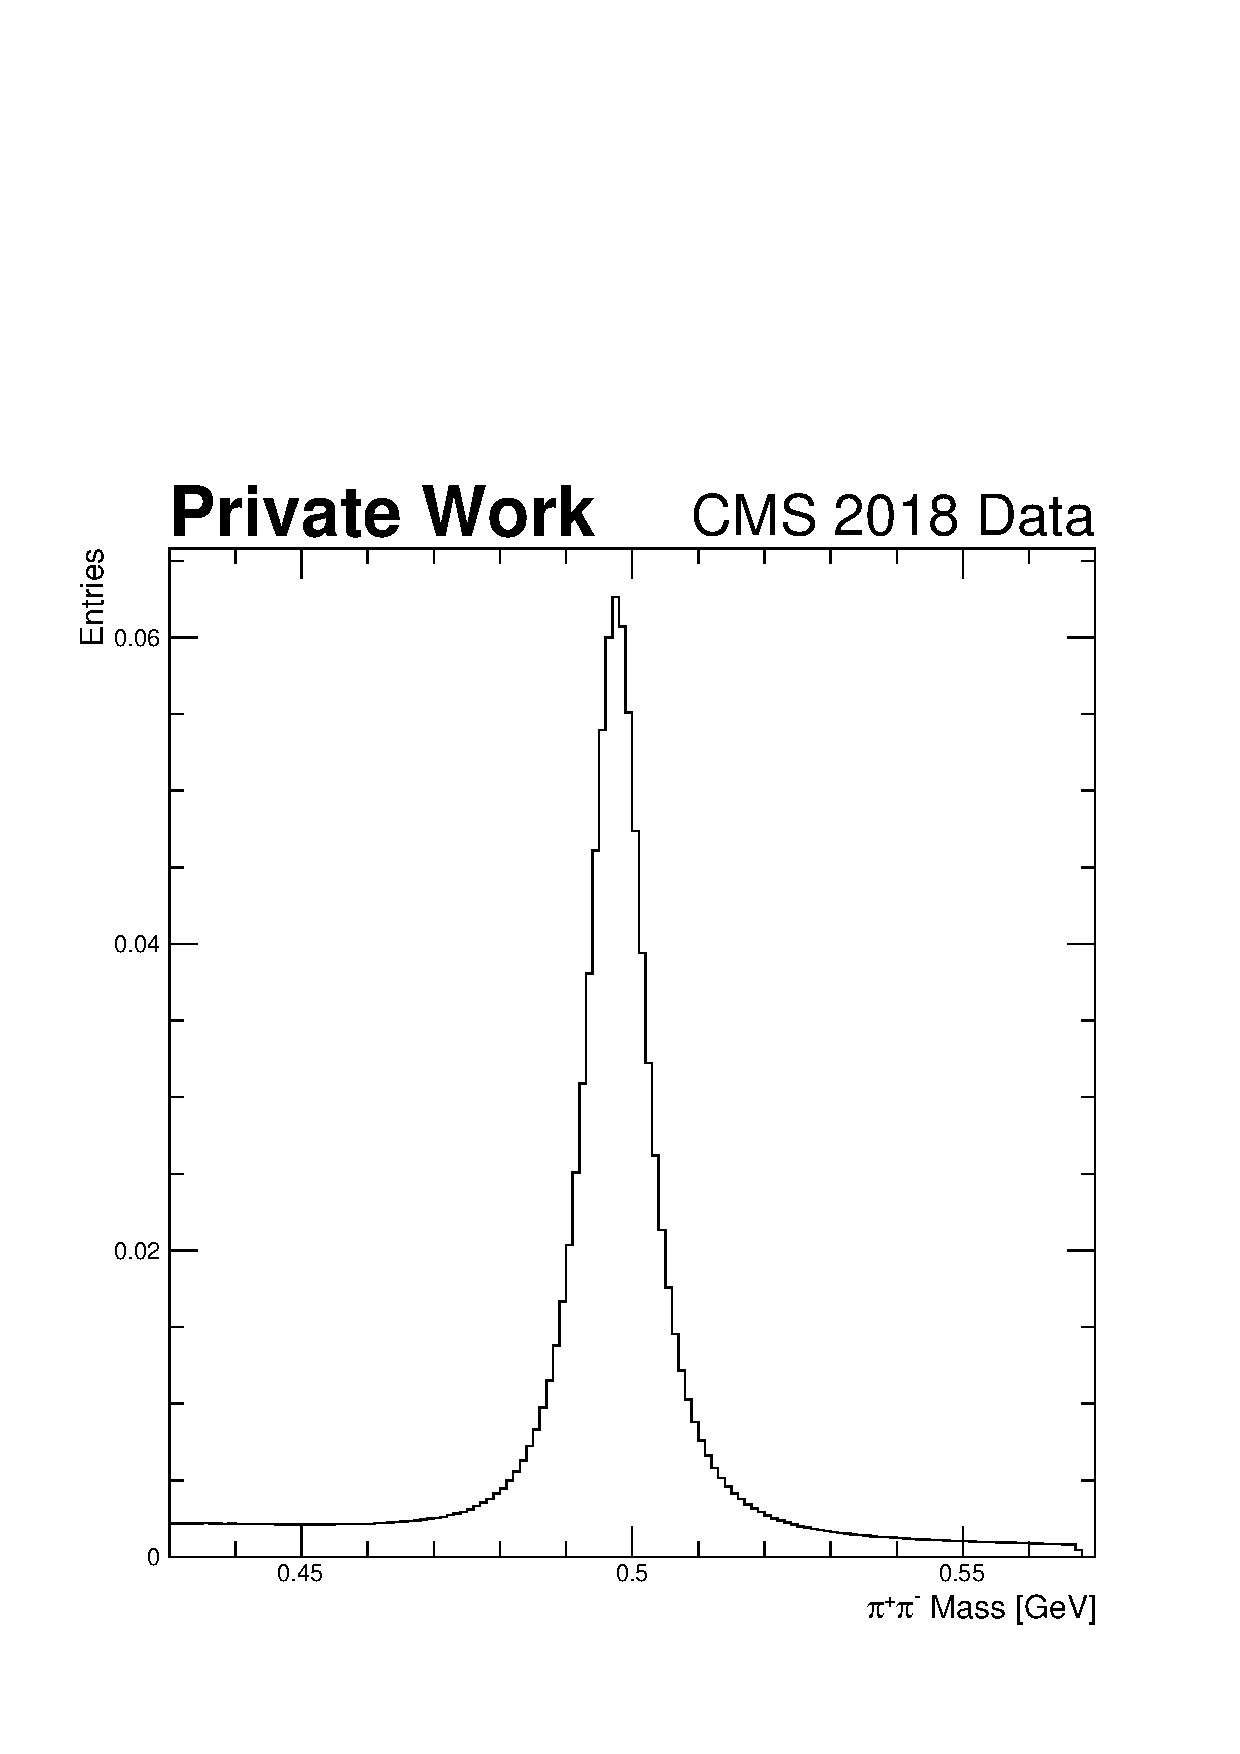
\includegraphics[height=8.5cm, width=9cm, trim= 0cm 0cm 0cm 0.cm,clip]{images/V0Candidates/DoubleMuon_UL2018_MiniAODv2_GT36-v1_hData_reco_K0_mass_.pdf}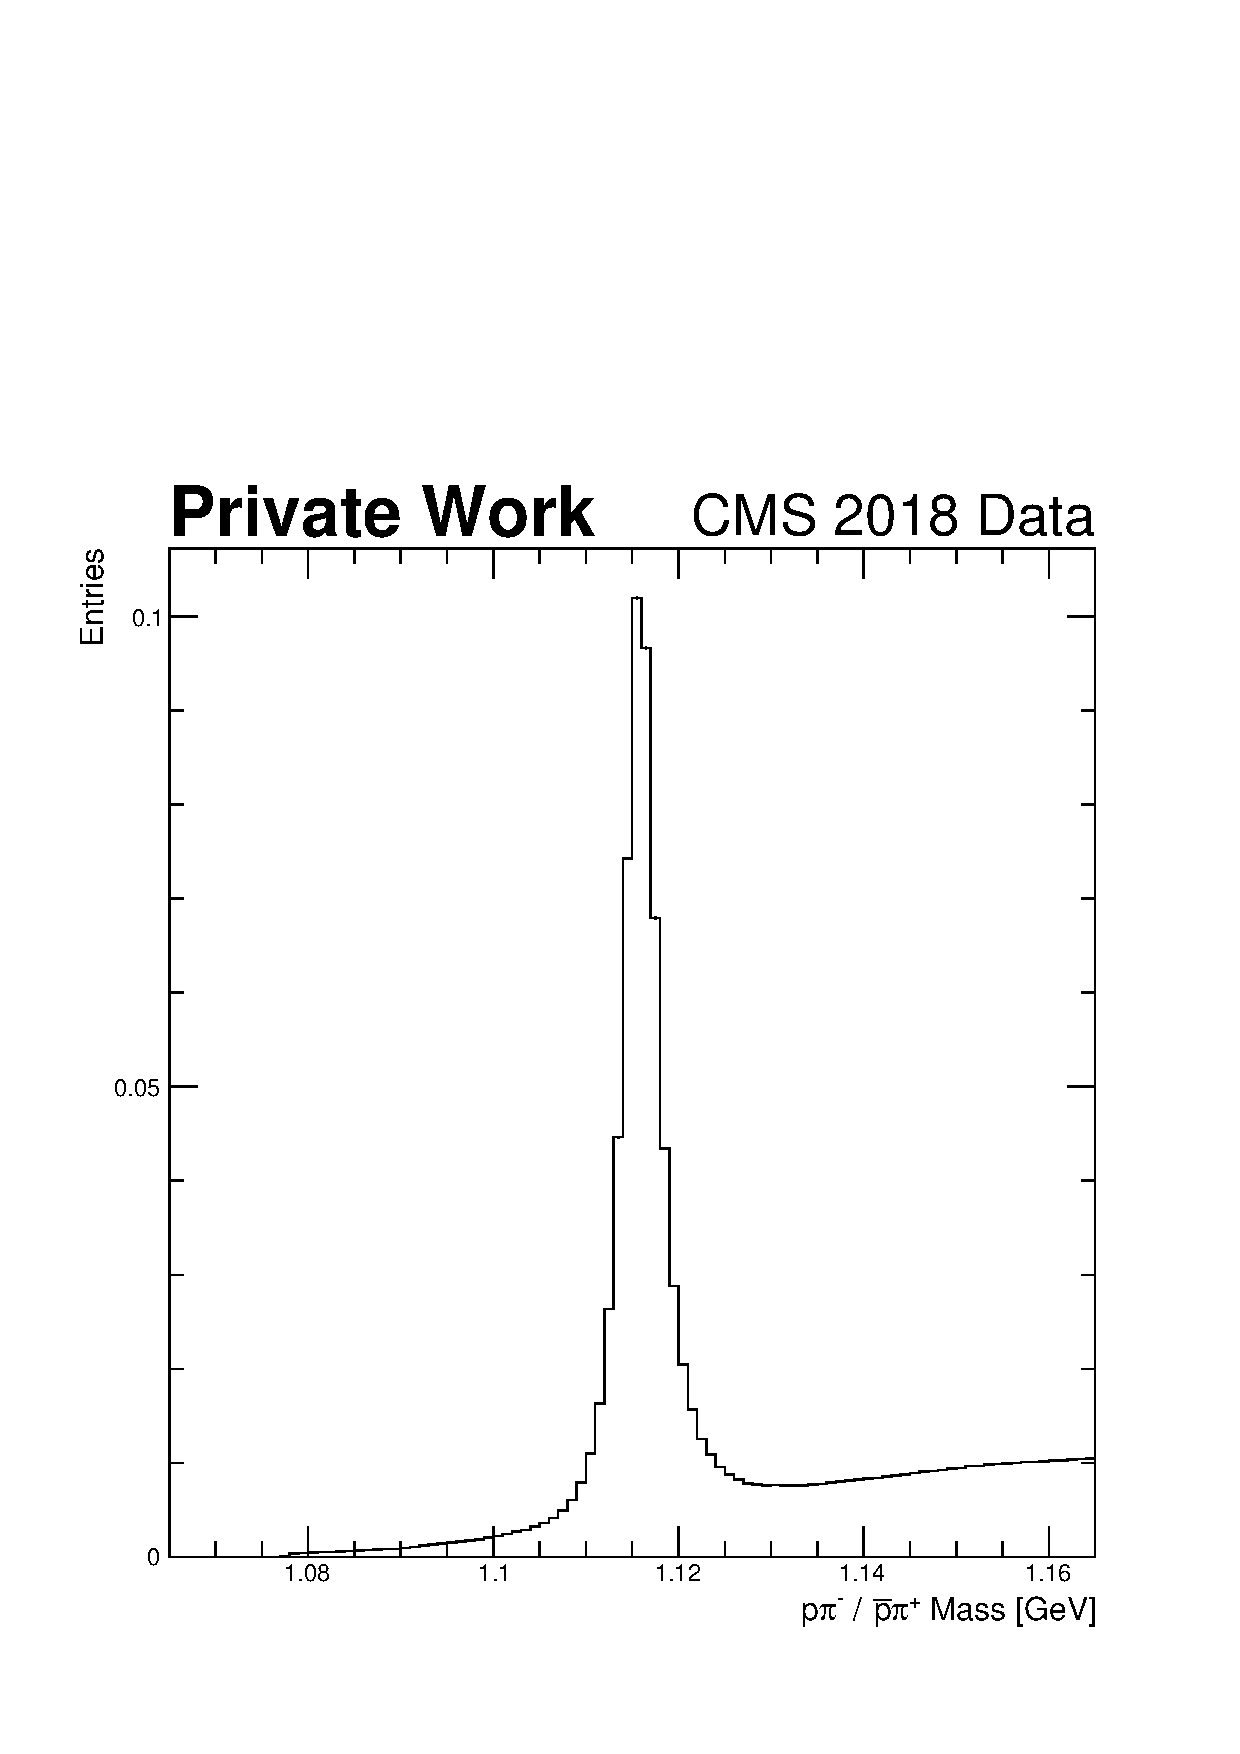
\includegraphics[height=8.5cm, width=9cm, trim= 0cm 0cm 0cm 0.cm,clip]{images/V0Candidates/DoubleMuon_UL2018_MiniAODv2_GT36-v1_hData_reco_L0_mass_.pdf}
\caption{\label{fig:V0Candidates} Mass plots of the V0 candidates from the DoubleMuon data sample of 2018}
\end{figure}


        
    \subsection{Tracks from Secondary Interactions}

        In order to remove the maximum of background tracks, the procedure of removing tracks associated to $V^0$ candidates vertices is extended to all kind of secondary interactions happening in the tracker volume, photon conversions and nuclear interactions with the material budget of CMS. The same algorithm is therefore used but now considering all kind of pair of tracks with selections detailed in Table \ref{tab:SECINTSEL}, that are specific for the reconstruction of such interactions.\\


    \begin{table}
        \centering
        \begin{tabular}{|c|c|}
        \hline
        \rowcolor{lightgray} 
           Variable  &  Cut\\
            \hline
            Nbr of tracks & 2 \\
            \hline
              Charge & SS or OS\\
             \hline
            $p_T$ & $>1$ GeV\\
            \hline
            $\frac{\chi^{2}_{trk}}{nDoF}$  & $<5$\\
            \hline
            $\frac{d_{xy}}{\sigma_{d_{xy}}}$ & $>5$\\
            \hline
             Inv. Mass & $<4$ GeV\\
            \hline
              $\frac{\chi^{2}_{vtx}}{nDoF}$ & $<20$\\
             \hline
        \end{tabular}
        \caption{Selections applied to the tracks and the secondary interaction vertex. Some selections are not mentioned but identical to the one used for V0 candidates.}
        \label{tab:SECINTSEL}
    \end{table}
            However, the veto applied on the pair of tracks belonging to secondary interactions is implemented differently.  In order to remove those tracks, we match the secondary interaction vertex position with the position of the layers of the tracker. These layers can be passive (Pixel Barrel inner and outer support, Pixel Barrel rails, beam pipe, ...) or active (Tracker Layers and Rings). The position of the active layers of the tracker is defined in the RECO data format where the first hit of the tracks is used to define each layer of the tracker, with the first hit of the tracks going up to the Tracker Outer Barrel Layer 1 (TOBL1), about 70 centimeters in the transverse plane from the center of CMS. The example for the Pixel Barrel is given in Fig.\ref{fig:trackermap}.\\
            For the passive layers, we take as a reference \cite{Sirunyan_2018} to define the position of the passive layers (therefore the veto we apply). Several passive layers are defined: the beam pipe, BPIX inner and outer support, BPIX rails, BPIX shields. It has been checked that this reference matches what is observed in MC for each year of Run 2.\\

            To avoid as much as possible secondary interaction vertices to be mistaken as signal vertices, an additional protection is applied by taking into account the vertex resolution in the width of the layers (passive and active). Since the vertex resolution decreases with respect to the distance to the center of CMS, the effective width of the layers can be extended from 0.05 mm for the first layers of pixels to almost 9 cm in the TEC disks.
            

\begin{figure}[ht]
\centering
\includegraphics[height=8cm, width=12cm, trim= 0cm 0cm 0cm 0cm,clip]{images/FirstHit/FirstHit_L1.pdf}
\caption{\label{fig:trackermap} Example of the tracker BPIXL1 geometry built using the RECO dataformat with the first hits of the tracks}
\end{figure}

\begin{figure}[ht]
\centering
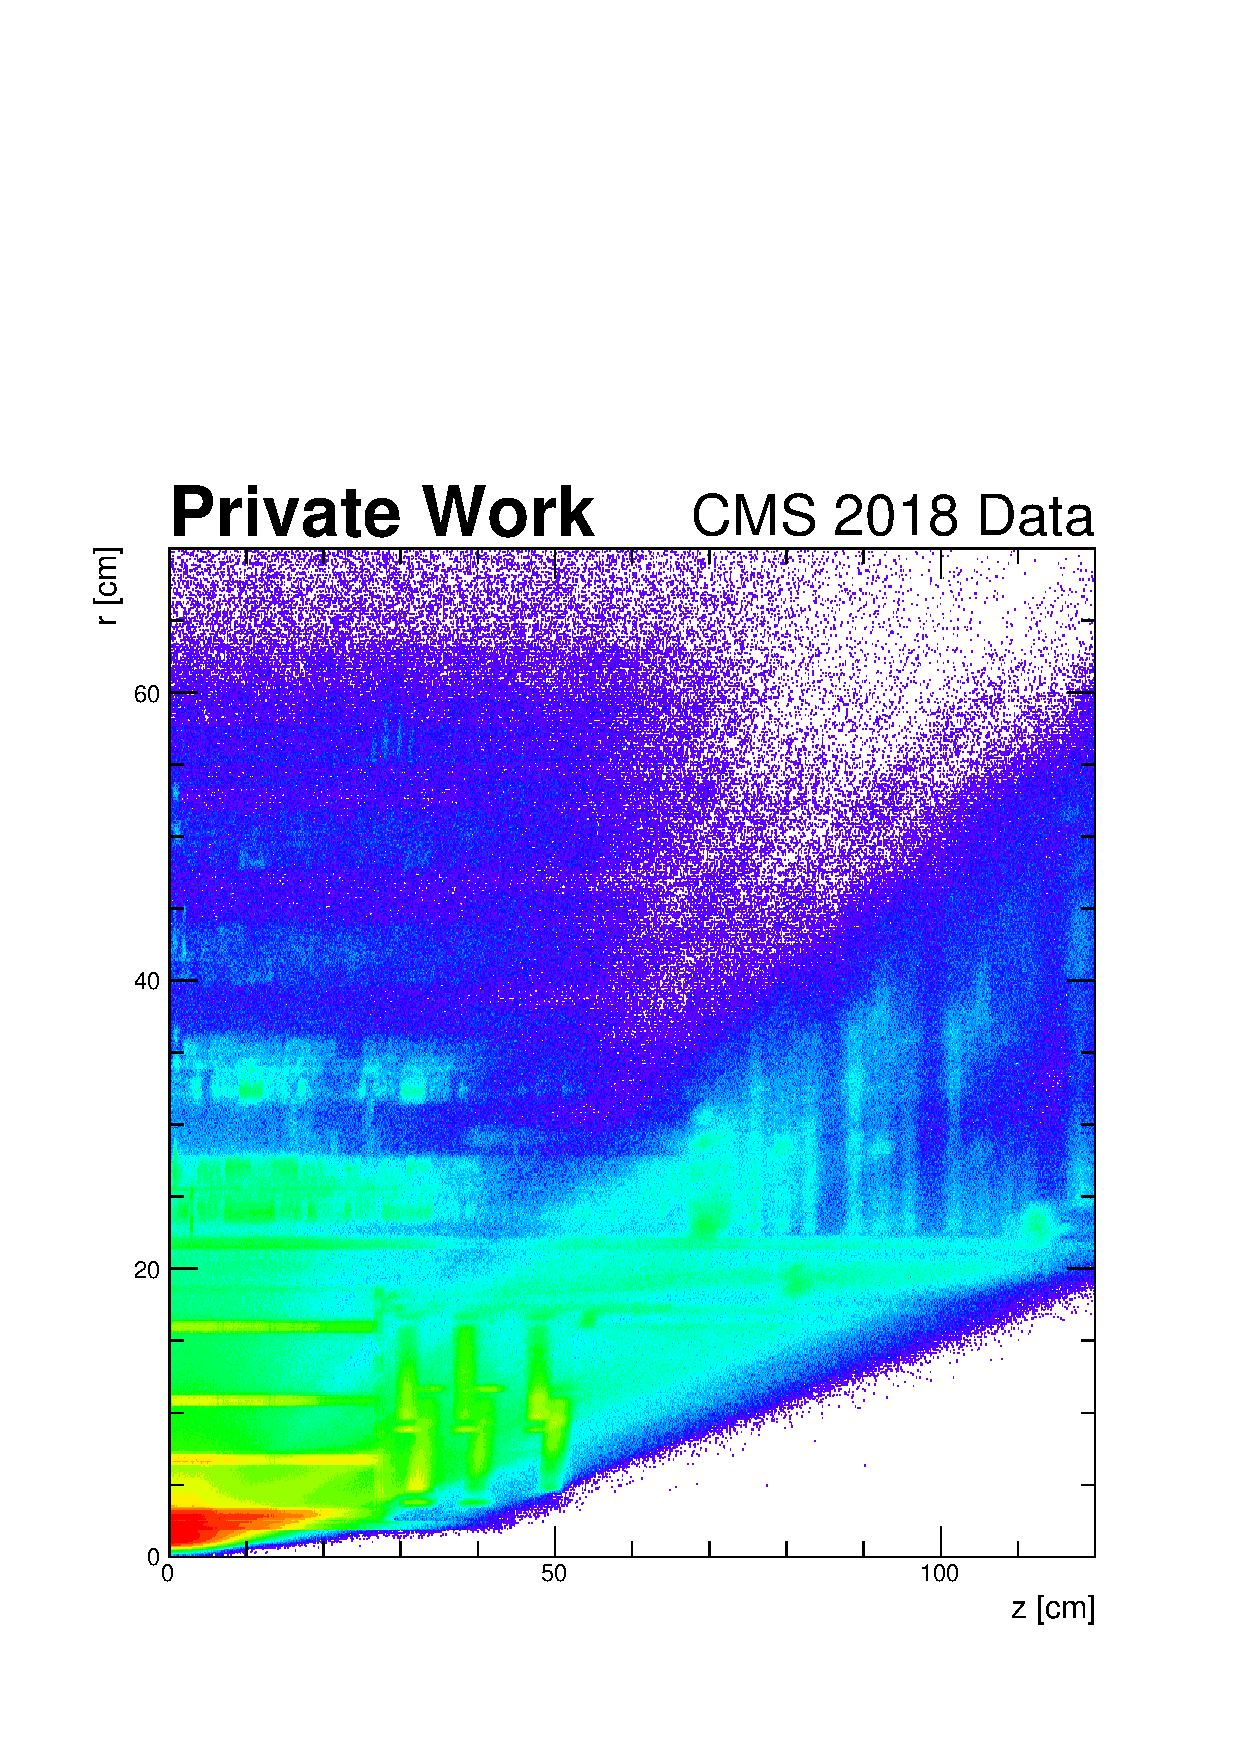
\includegraphics[height=9cm, width=9cm, trim= 0cm 0cm 0cm 0.cm,clip]{images/SecInt/DoubleMuon_UL2018_MiniAODv2_GT36-v1_hData_reco_SecInt_rz_Selec.pdf}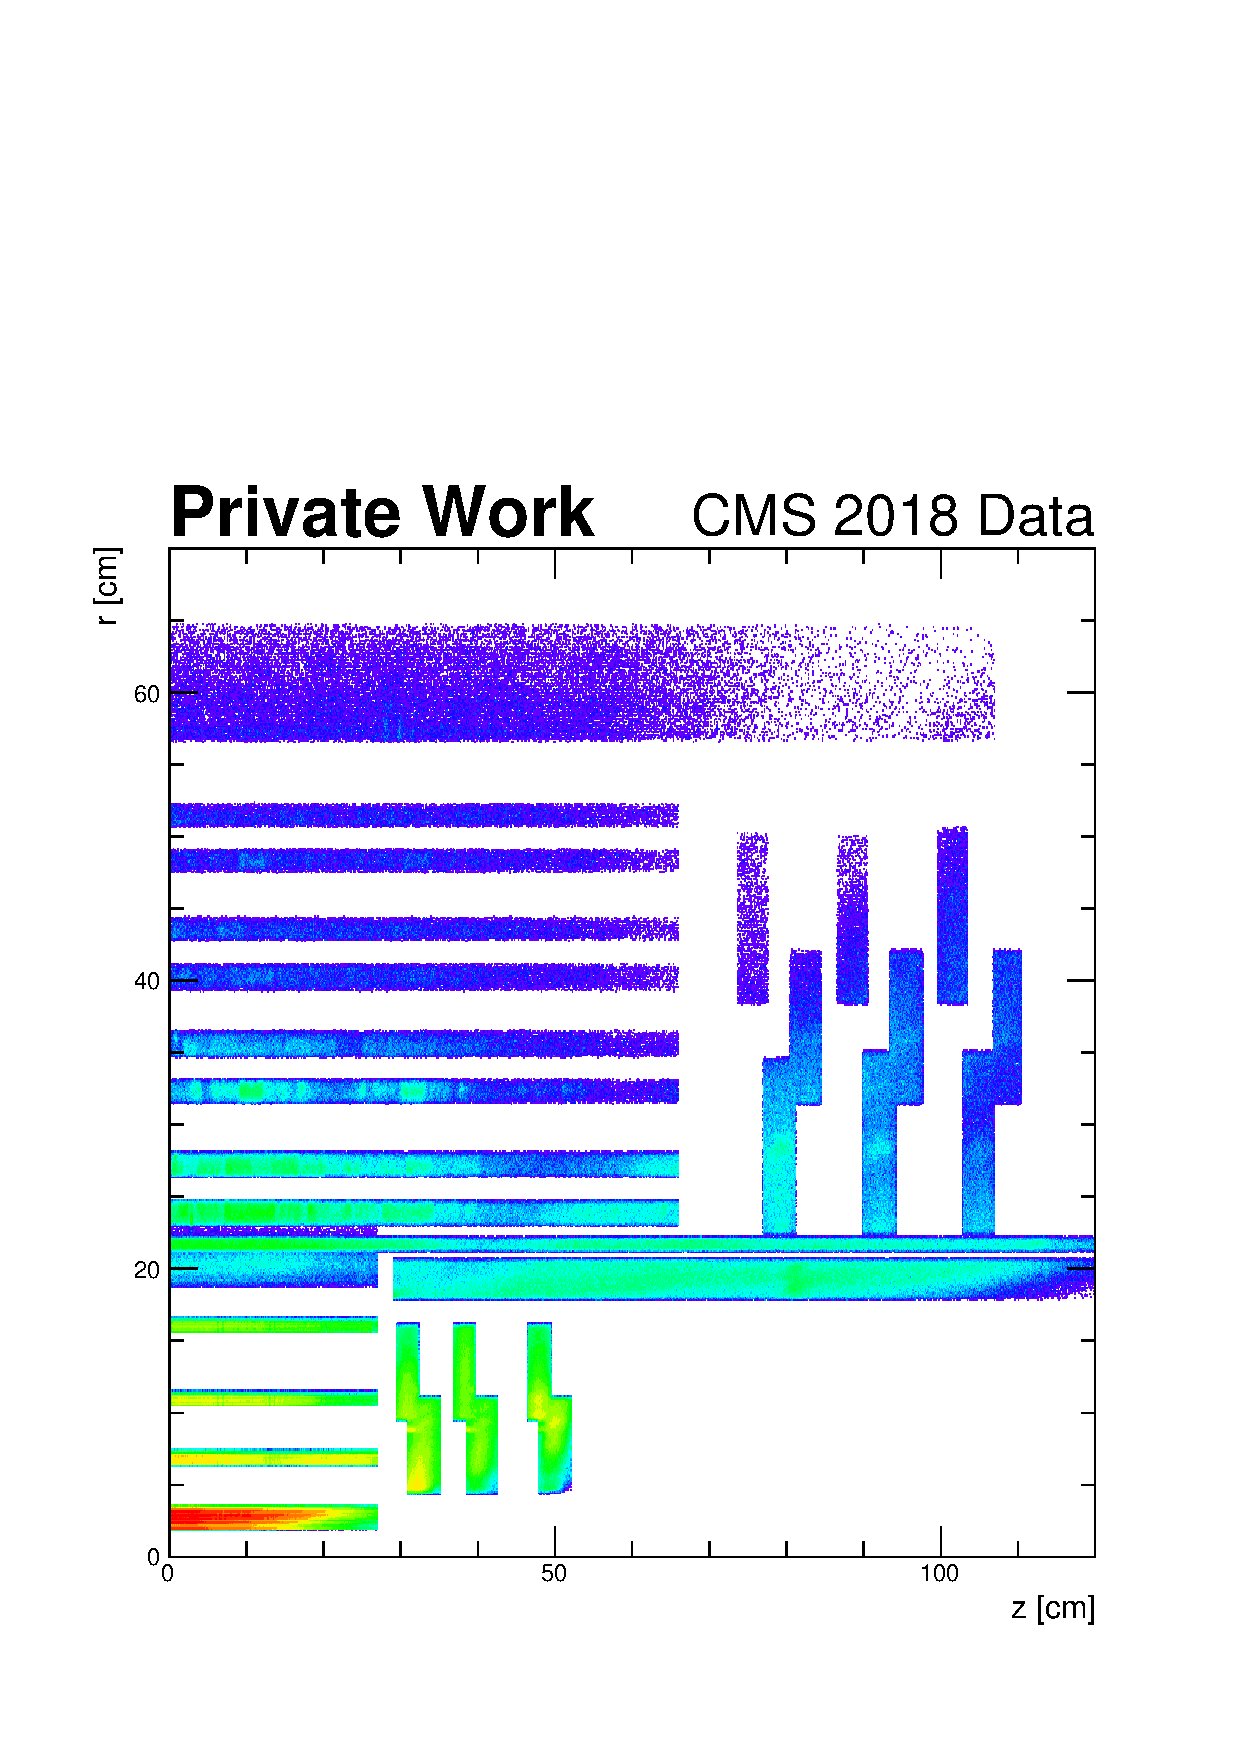
\includegraphics[height=9cm, width=9cm, trim= 0cm 0cm 0cm 0.cm,clip]{images/SecInt/DoubleMuon_UL2018_MiniAODv2_GT36-v1_hData_reco_SecInt_rz_TrackerMatched.pdf}
\caption{\label{fig:longVeto} Longitudinal distribution of secondary interactions for the DoubleMuon data sample}
\end{figure}

\begin{figure}[ht]
% \centering
\hspace{-1 cm}
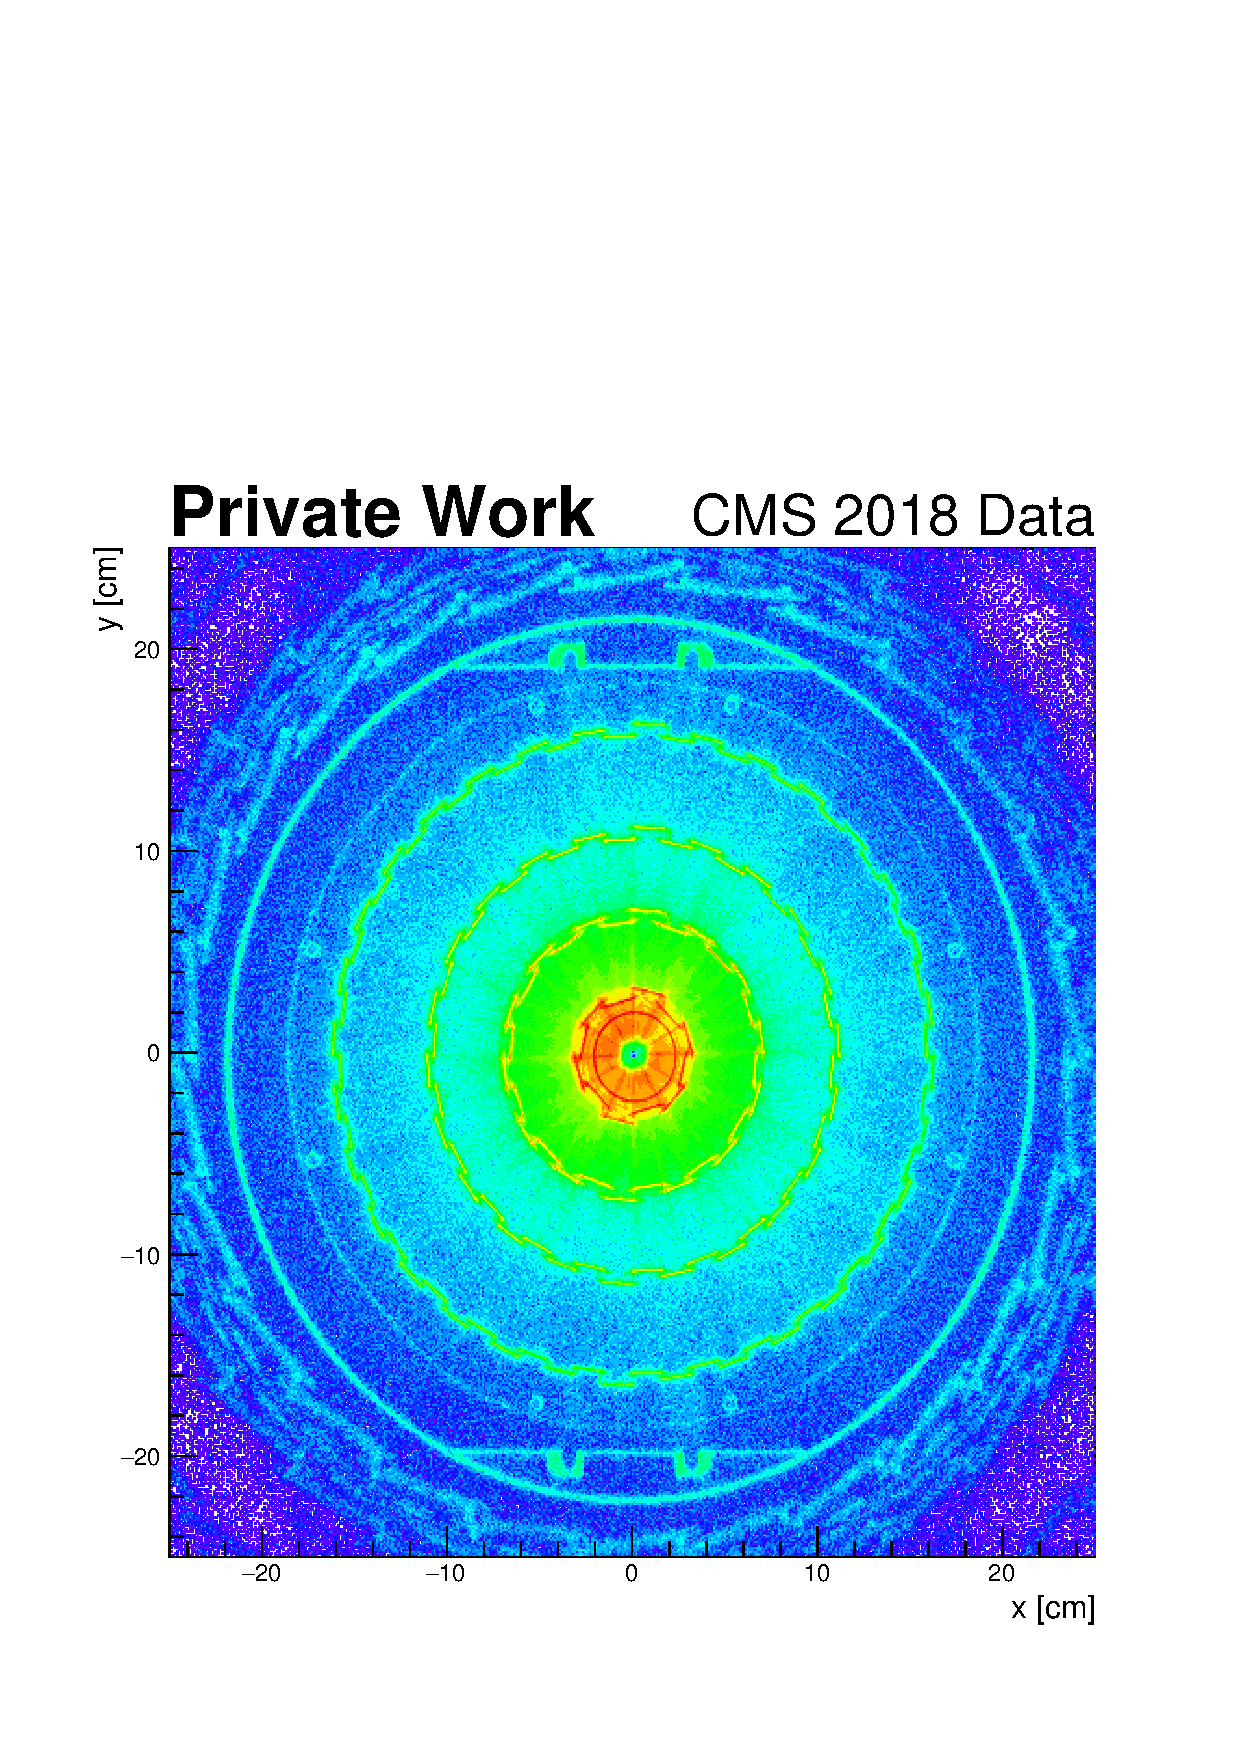
\includegraphics[height=9cm, width=9cm, trim= 0cm 0cm 0cm 0.cm,clip]{images/SecInt/DoubleMuon_UL2018_MiniAODv2_GT36-v1_hData_reco_SecInt_xy_Selec.pdf}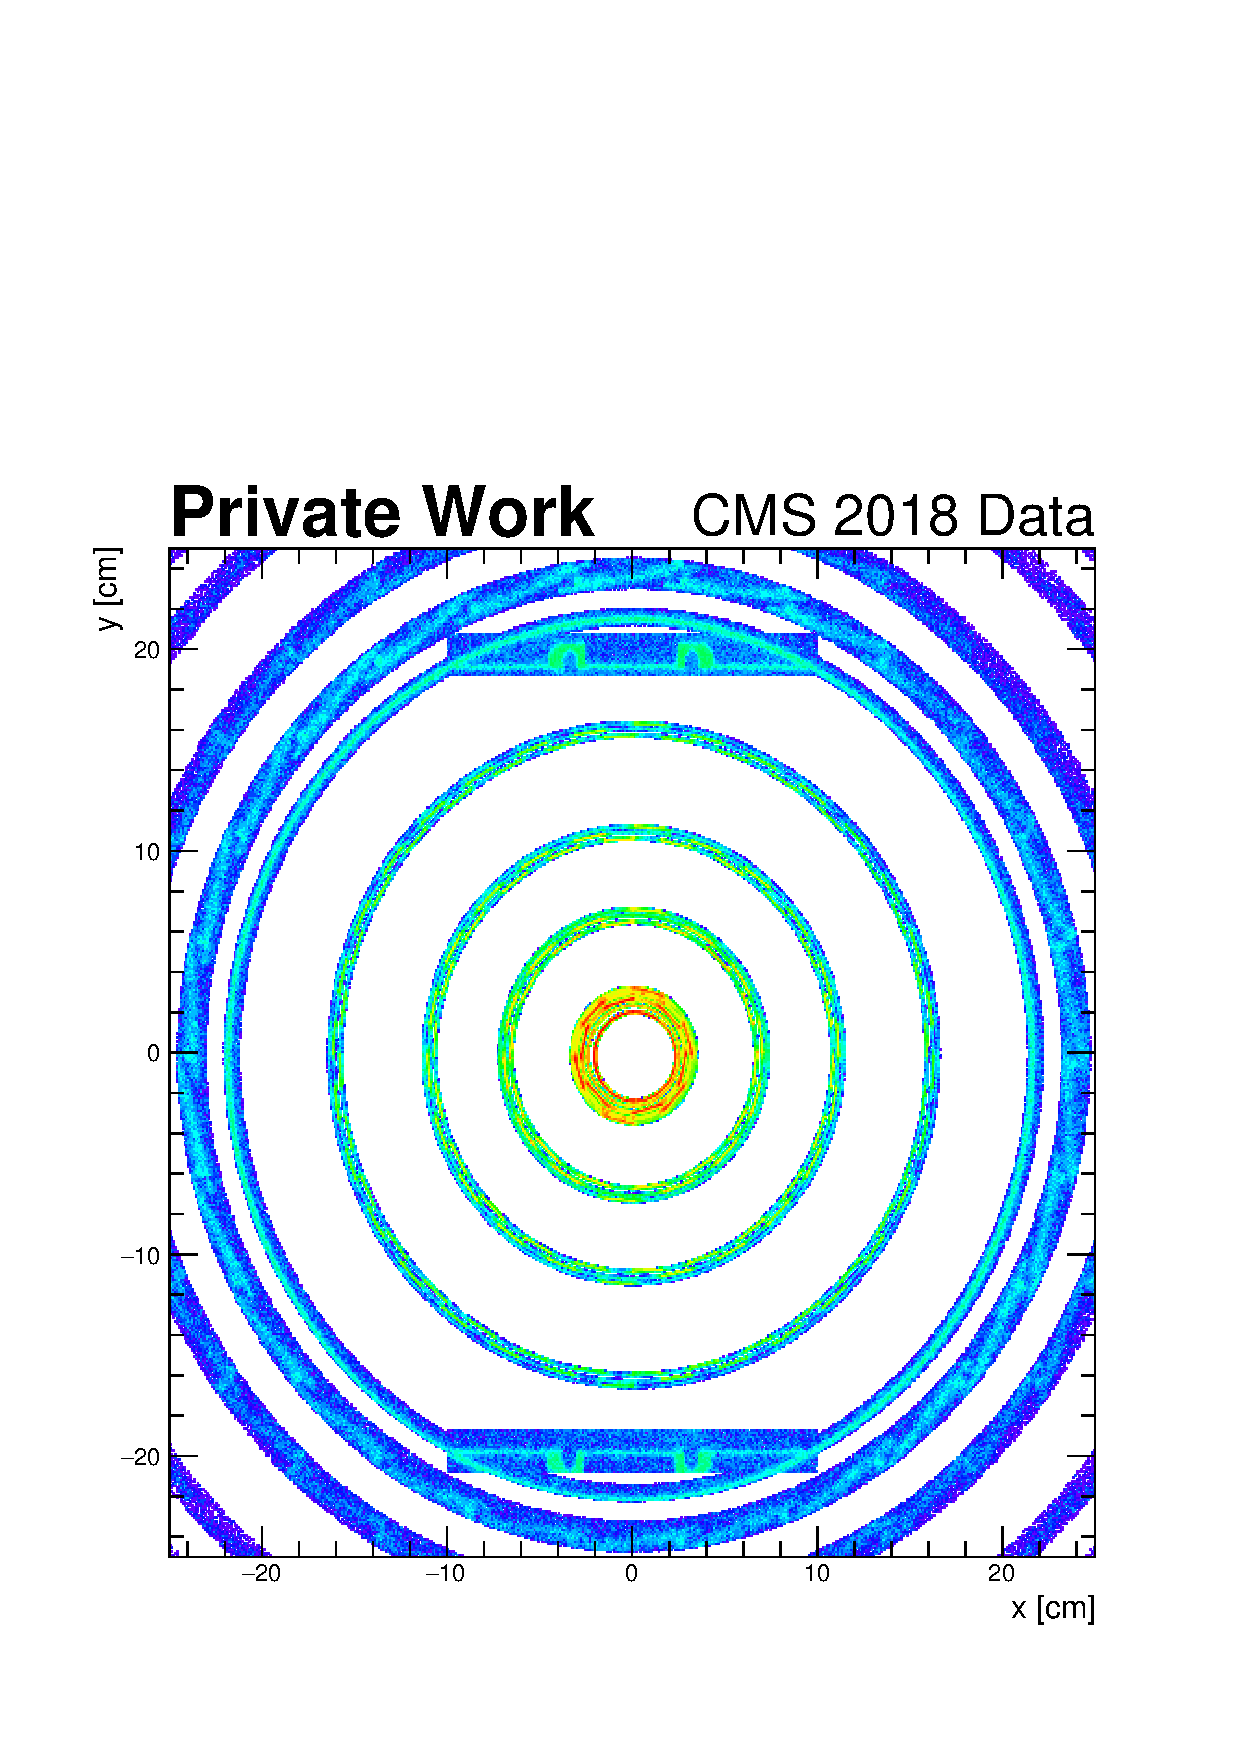
\includegraphics[height=9cm, width=9cm, trim= 0cm 0cm 0cm 0.cm,clip]{images/SecInt/DoubleMuon_UL2018_MiniAODv2_GT36-v1_hData_reco_SecInt_xy_TrackerMatched.pdf}
\caption{\label{fig:Veto} Transverse distribution of secondary interactions for the DoubleMuon data sample}
\end{figure}

\begin{figure}[ht]
% \centering
\hspace{-1 cm}
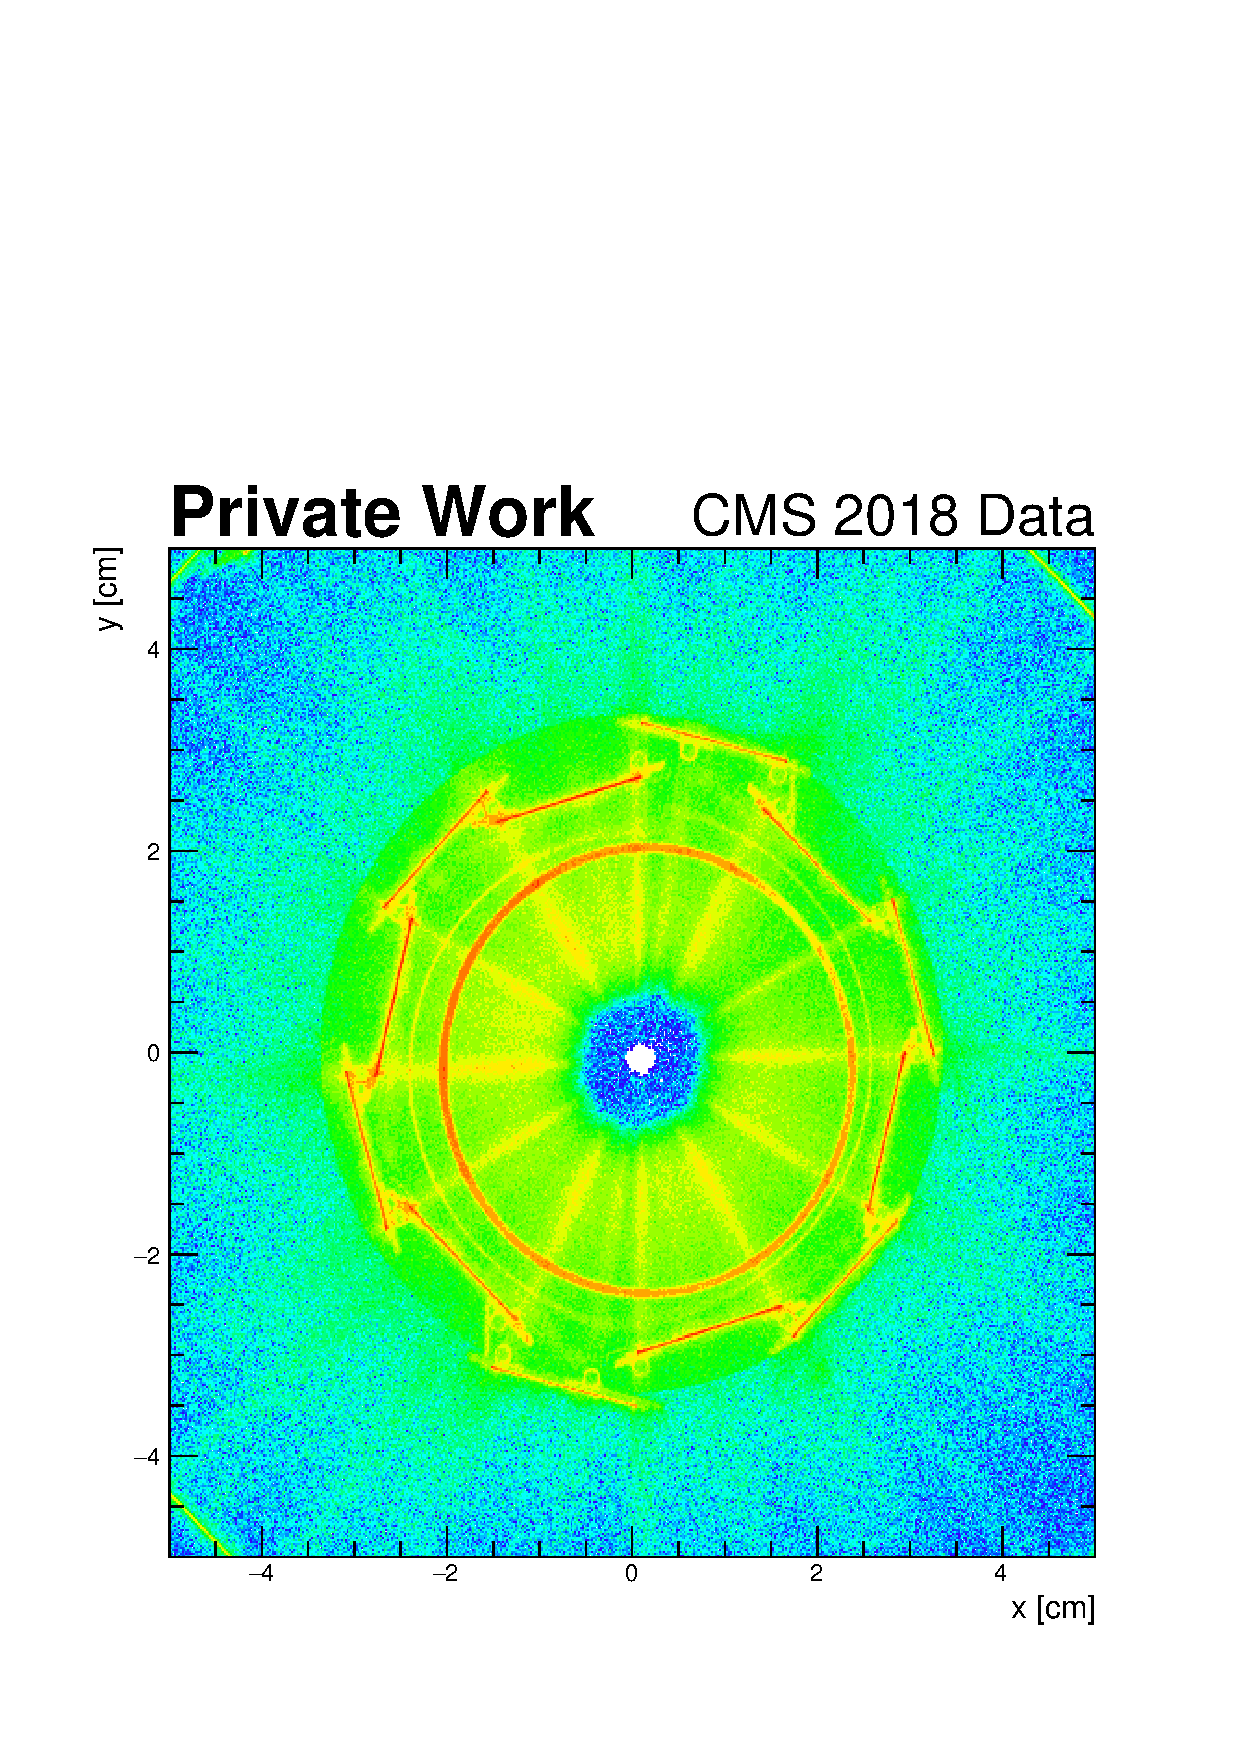
\includegraphics[height=9cm, width=9cm, trim= 0cm 0cm 0cm 0.cm,clip]{images/SecInt/DoubleMuon_UL2018_MiniAODv2_GT36-v1_hData_reco_SecInt_xy_Inner_Selec.pdf}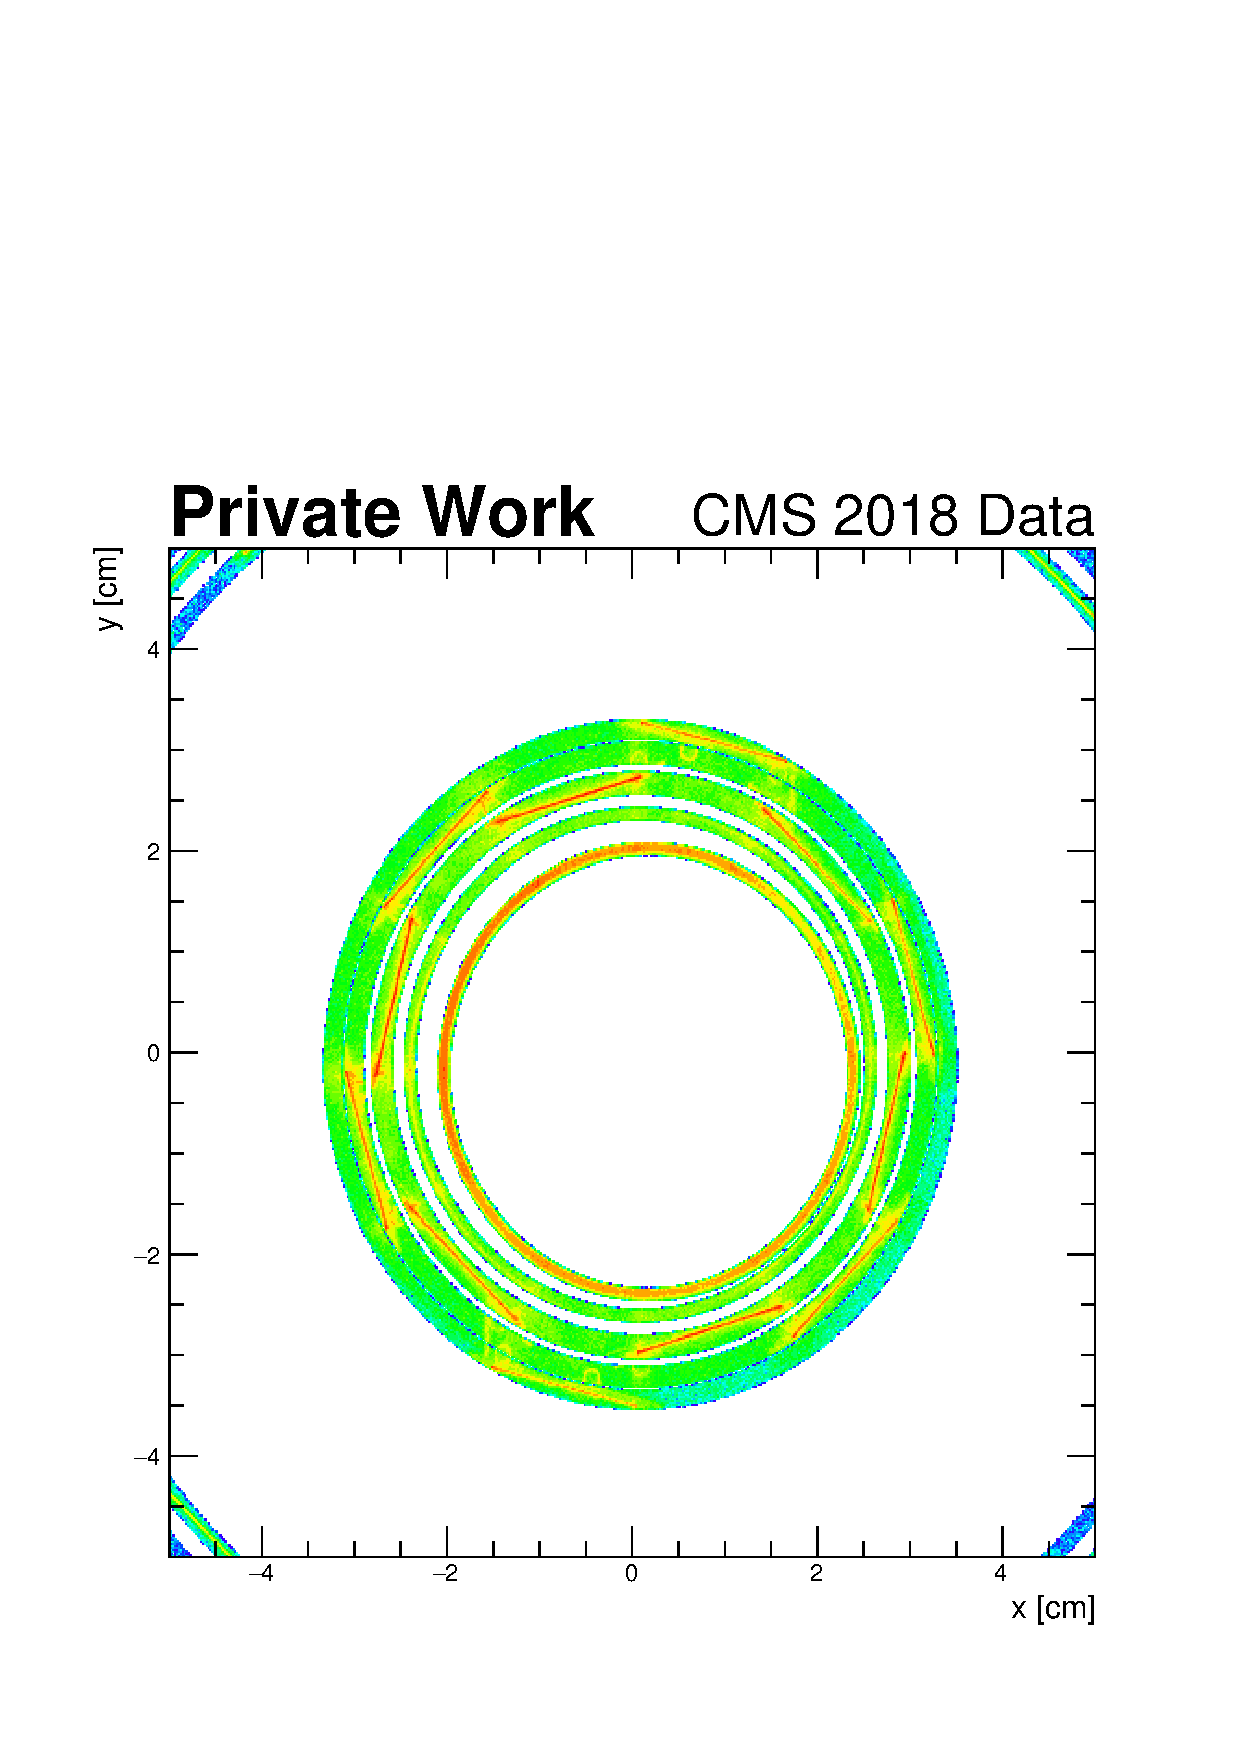
\includegraphics[height=9cm, width=9cm, trim= 0cm 0cm 0cm 0.cm,clip]{images/SecInt/DoubleMuon_UL2018_MiniAODv2_GT36-v1_hData_reco_SecInt_xy_Inner_TrackerMatched.pdf}
\caption{\label{fig:InnerVeto} Transverse distribution of secondary interactions in the inner part of the tracker for the DoubleMuon data sample}
\end{figure}
        \FloatBarrier

    Once the matching is done between the two positions, the tracks associated to the secondary interactions are removed from the workflow. The applied veto is shown in Fig.\ref{fig:longVeto}, Fig.\ref{fig:Veto} and  Fig.\ref{fig:InnerVeto}.
        
    \subsection{Tracks from signal}
        \label{SUB:BDTRK}
        \subsubsection{MiniAOD track constraints}
        Since the analysis is performed in the MiniAOD data format, there are several flags that have to be taken care of. The first one is that in this analysis, both packedPFCandidate and lostTracks collections are considered, more details in \cite{MiniAOD}. Indeed, one can expect displaced tracks to be of worse quality compared to prompt tracks and to be part of the lostTracks collection (not assigned to any PF candidate). The use of MiniAOD data-format also induces the use of High Purity tracks  (mva-based quality criteria using $p_T$ relative error, $\eta$, $\chi^2$, number of hits and number of lost hits). $\sim 97.8$\% of the tracks are HighPurity ones for all signal samples and $\sim$ 90\% in a $t\bar{t}$ MC sample and 88\% in a DY MC sample. The final requirement of the tracks are that lostTracks collection is added without requiring the HighPurity flag on (all tracks are not exaclty high-purity tracks) to keep the maximum of tracks before applying any selection. As a note, most tracks that will be selected by the track selection BDT (see below) are HighPurity tracks ($\sim$ 99\% for all the signal samples and 95\% for a $t\bar{t}$ sample and 94\% for a DY sample).

        % \begin{table}[h]
        %     \centering
        %         \begin{tabular}{|m{4cm}|m{3.cm}|m{3.5cm}|m{3cm}|}
        %             \hline
        %             \rowcolor{lightgray} 
        %              \centering Selection & Signal Track selection efficiency & Bkg track selection efficiency (in Signal Events) & $t\Bar{t}$ track selection efficiency\\
        %             \hline
        %             With LostTracks and without HighPurity flag on &  94.5 & 10 & 6.5 \\
        %             \hline
        %             With LostTracks and HighPurity flag on & 93.3 & 8.7 &  5.4 \\
        %             \hline
        %             Without LostTracks and without HighPurity flag on & 81.5 & 8 & 4.9\\
        %             \hline
        %             Without LostTracks and with HighPurity flag on & 81.4 & 8 & 4.9\\
        %             \hline
        %         \end{tabular}
        %     \caption{Track selection efficiency as a function of track quality flags}
        %     \label{tab:TRKSEL}
        % \end{table}
        
        Tracks from the neutralino have a displacement that depends on the decay length of the latter, and it can be possibly hard to distinguish background tracks from signal tracks depending on the phase space. A first selection is optimised to reduce the number of background tracks by requiring $p_T > 1$ GeV, $\frac{\chi^2}{dof} < 5$ and a transverse impact parameter significance $|\frac{d_{xy}}{\sigma_{xy}}| > 5$ where  $\sigma_{xy}$ is the error on $d_{xy}$. Fig.\ref{fig:TRKDis} shows the distribution of these 3 variables after the cut between signal and $t\bar{t}$ events. This pre-selection allows to reduce a significant amount of background (about 90\% for $t\Bar{t}$) while keeping 95\% of the signal displaced tracks. \\

        \begin{figure}[ht]
        \centering
        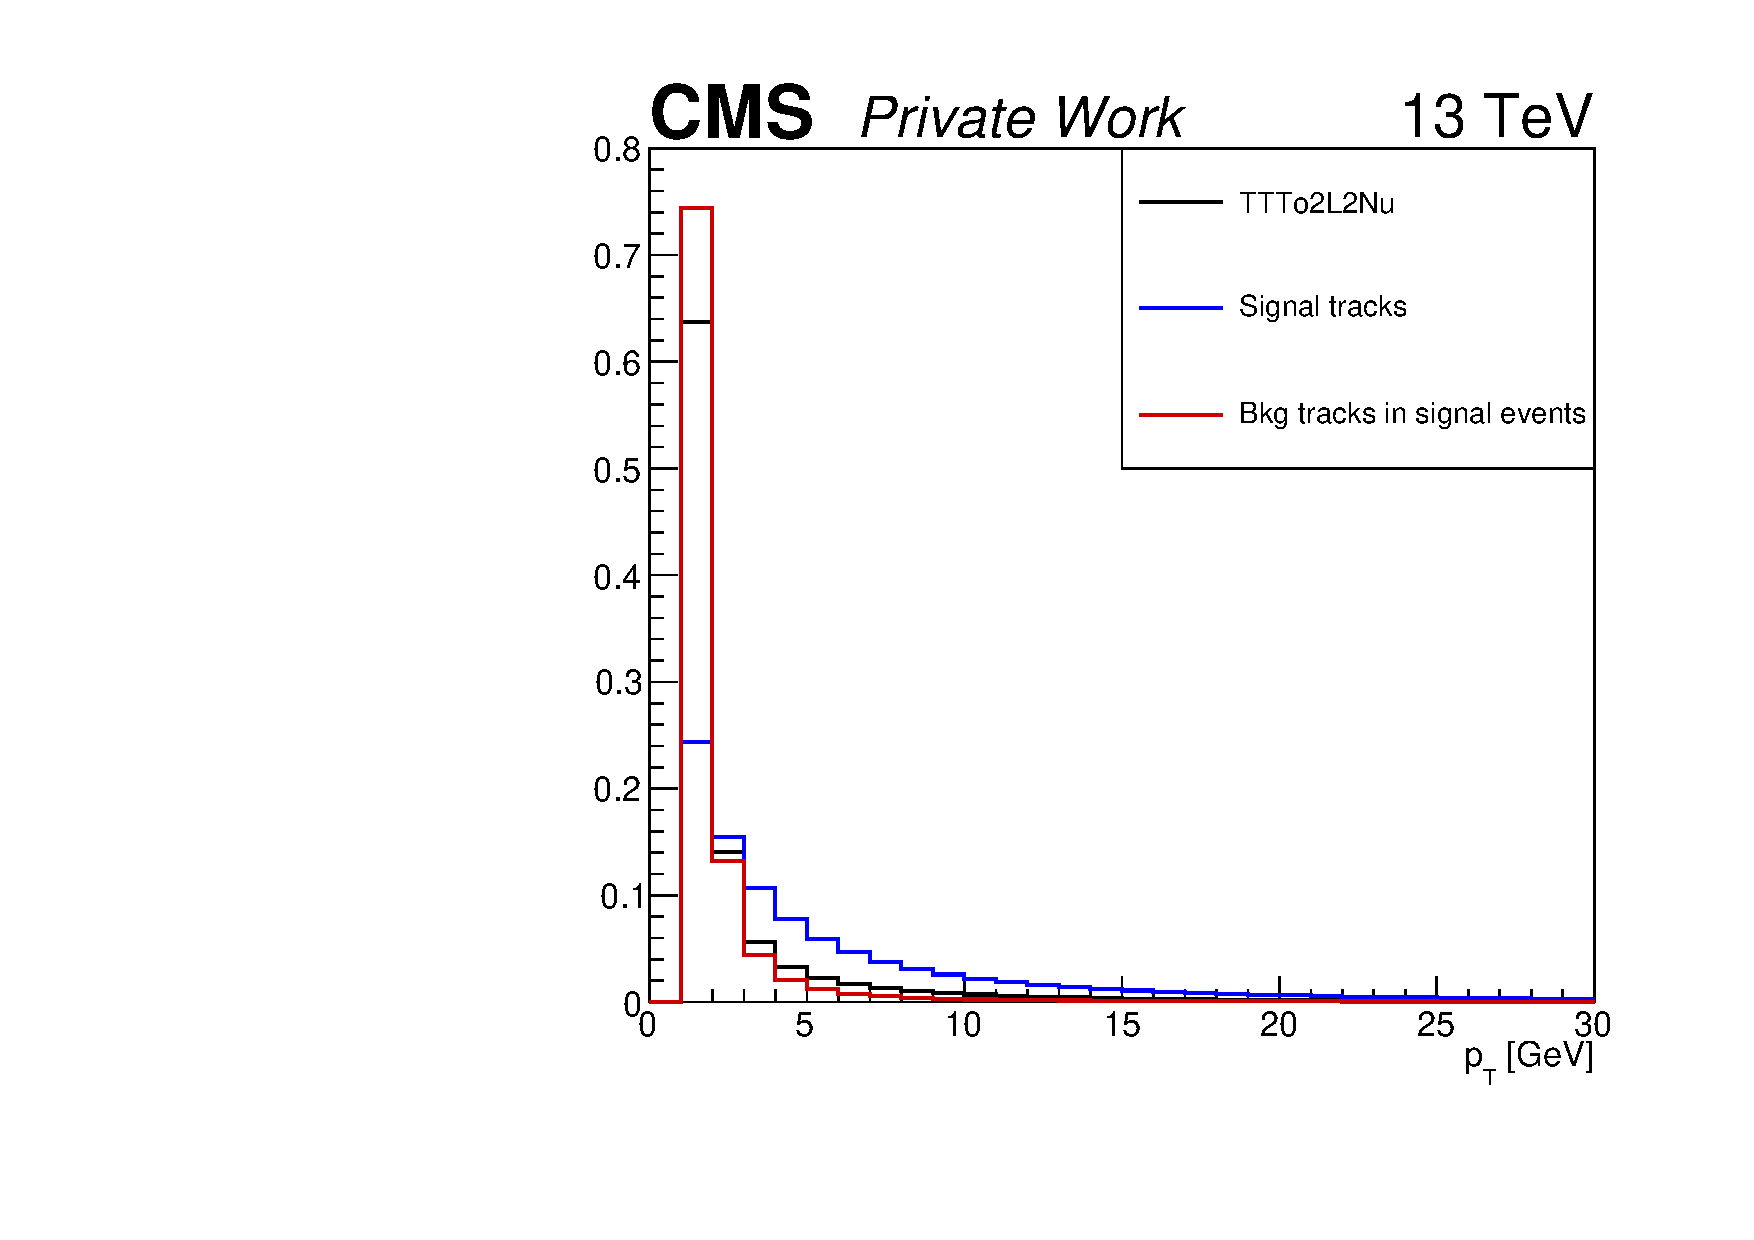
\includegraphics[height=8cm, width=8cm, trim= 0cm 0cm 0cm 0cm,clip]{images/TRK/Pt_TT.pdf}
        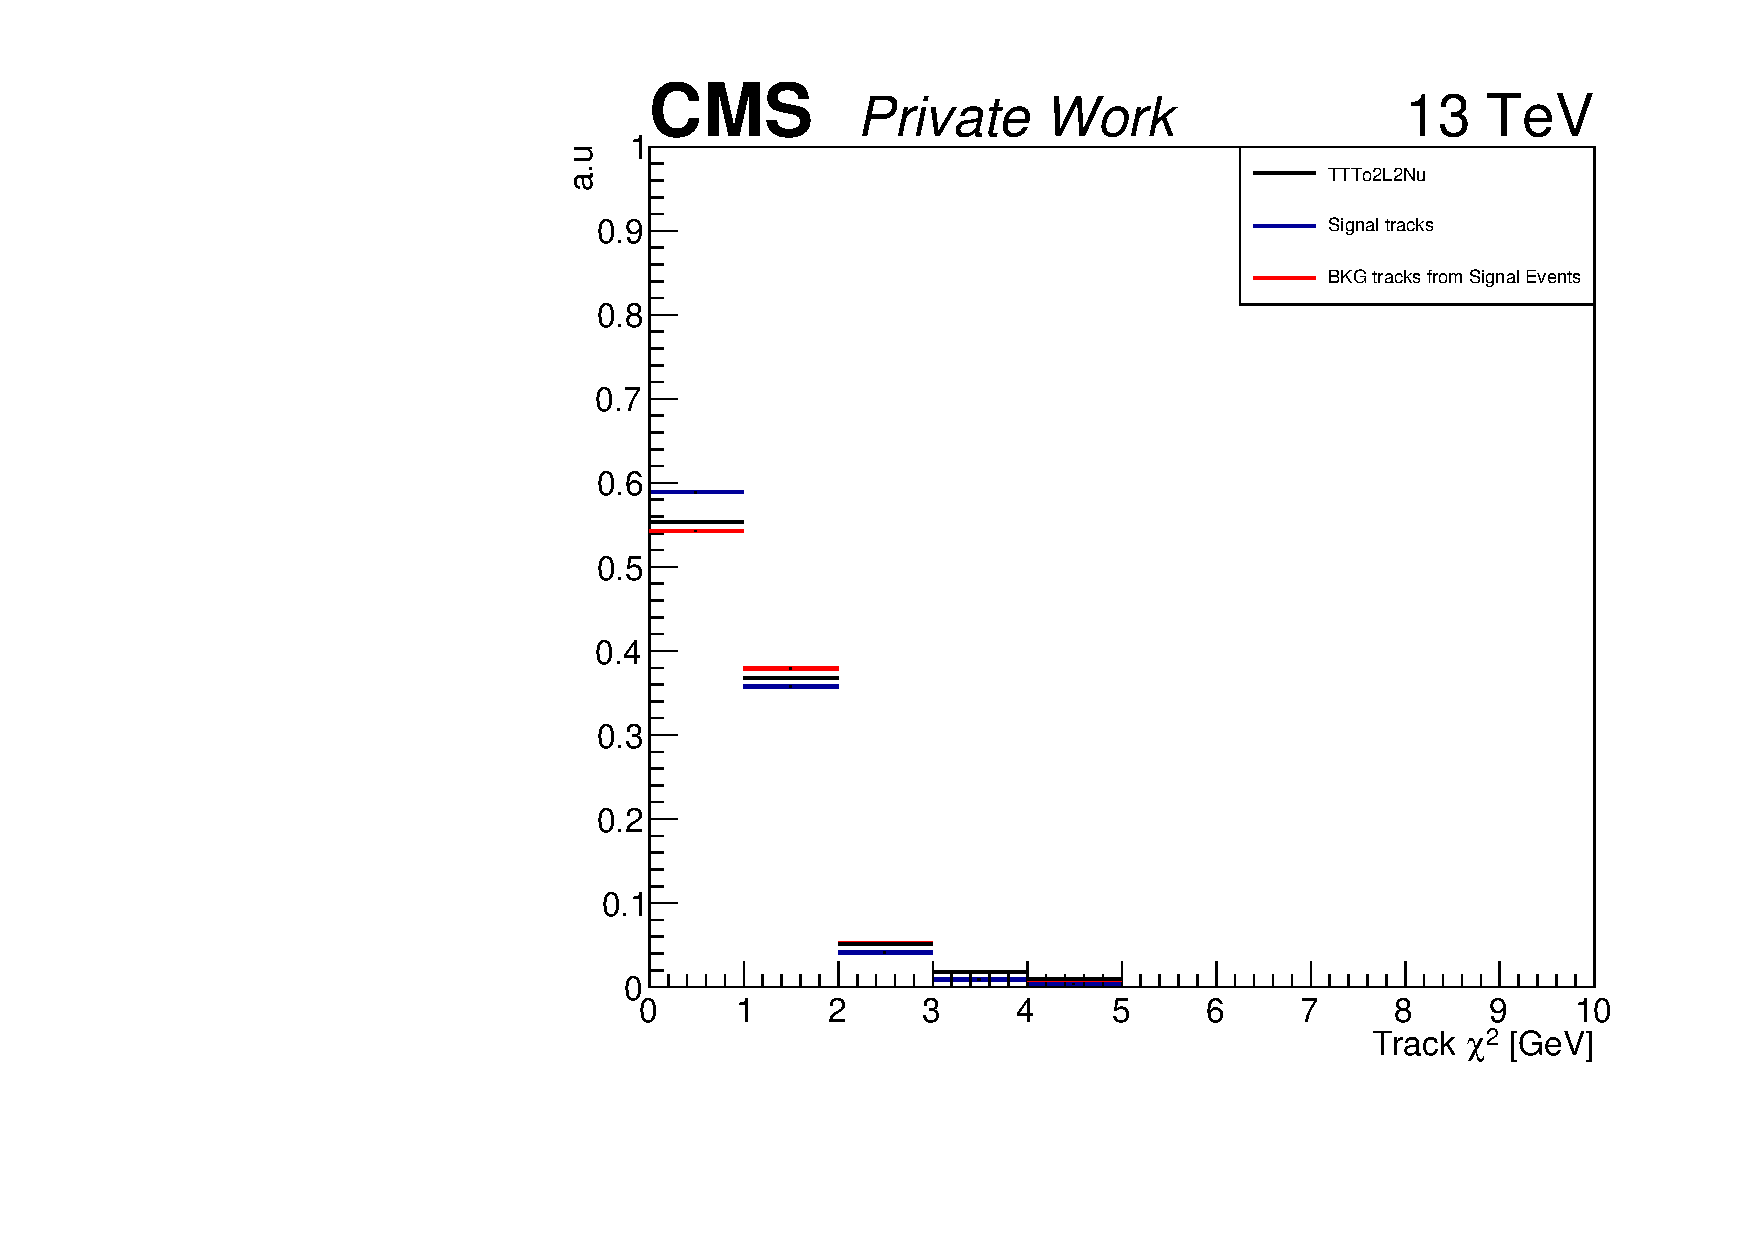
\includegraphics[height=8cm, width=8cm, trim= 0cm 0cm 0cm 0cm,clip]{images/TRK/Track_chi2.pdf}
        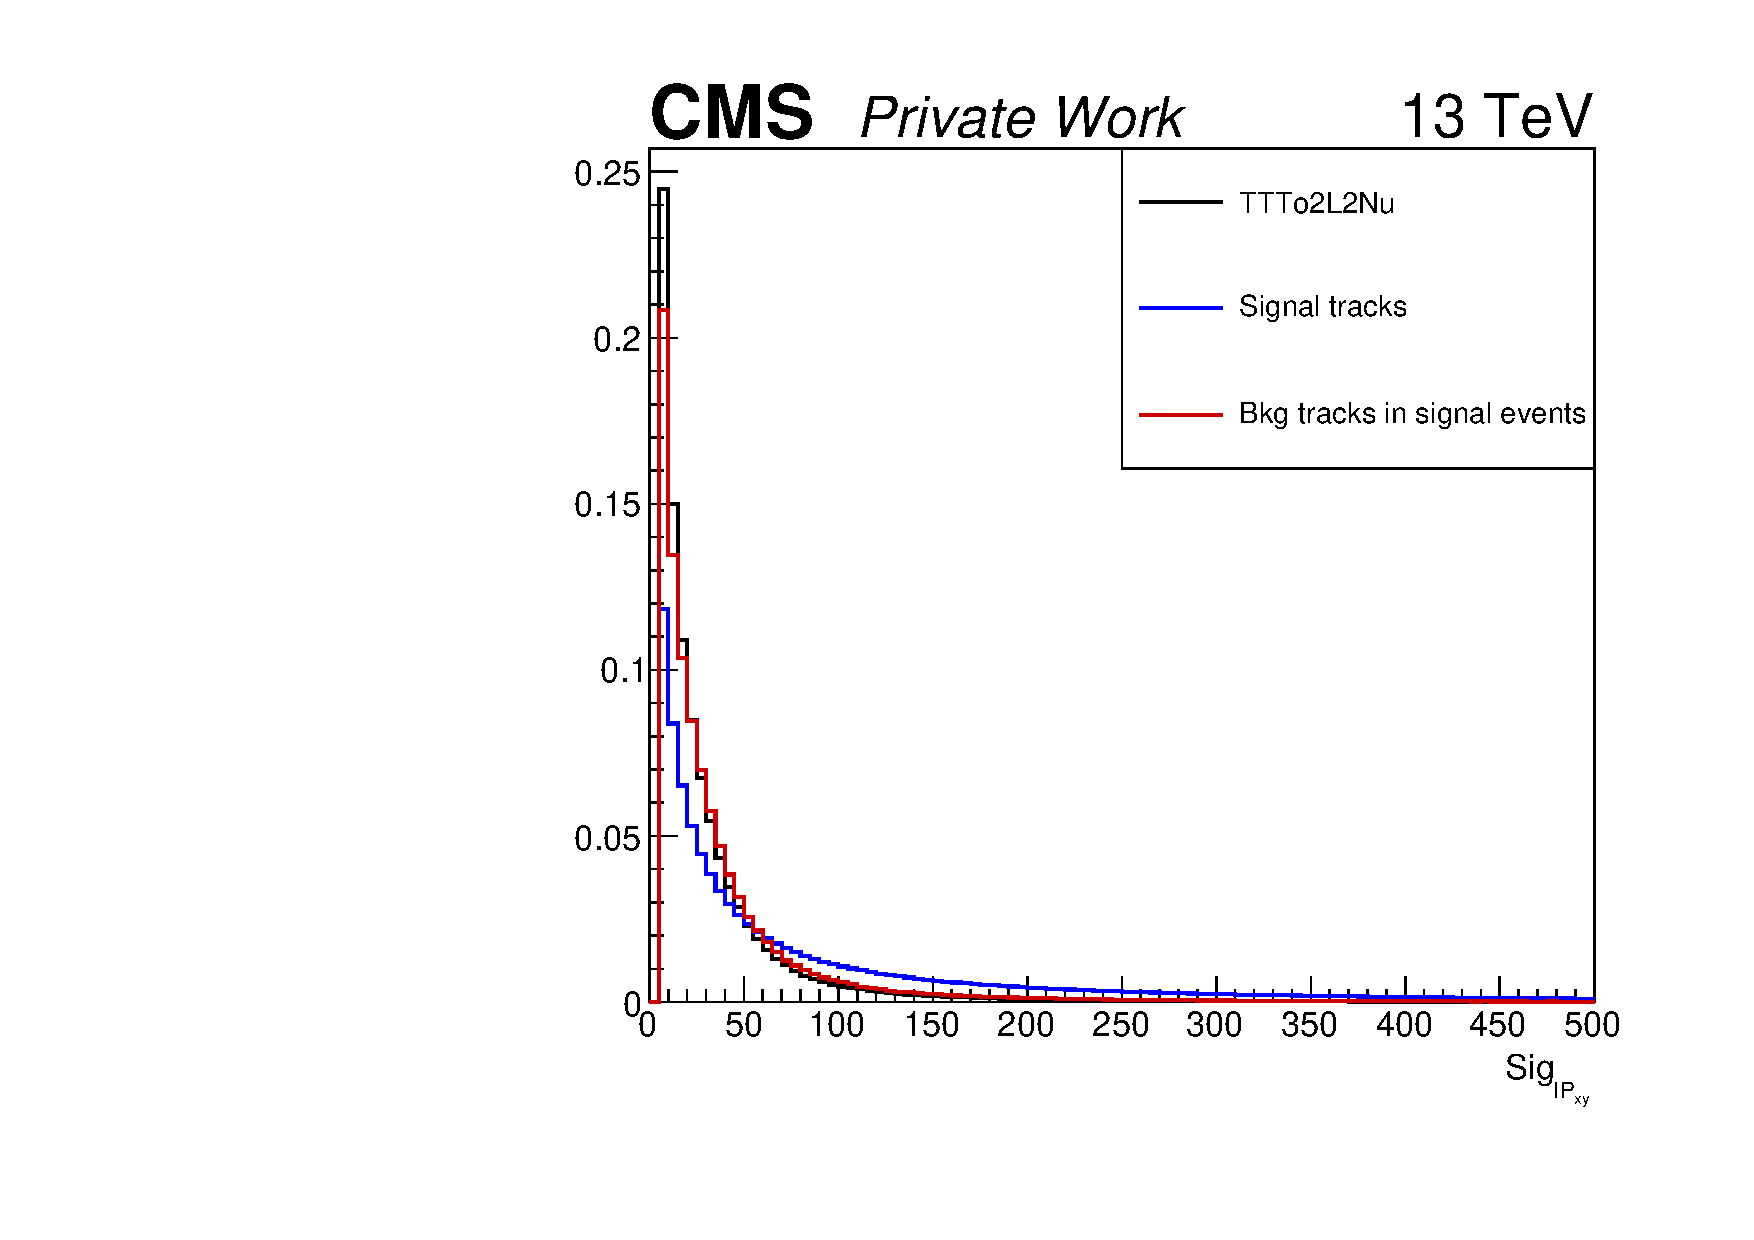
\includegraphics[height=8cm, width=8cm, trim= 0cm 0cm 0cm 0cm,clip]{images/TRK/drSig_TT.pdf}
        \caption{\label{fig:TRKDis} Track $p_T$, $\frac{\chi^2}{nDoF}$ and impact parameter distributions. Distributions are shown for signal tracks, background tracks in signal events and tracks from $t\bar{t}$. }
        \end{figure}

        \FloatBarrier


        \subsubsection{Boosted Decision Tree for track selection}
        However, these first cuts do not allow to reduce the background at a high enough amount to observe the signal, therefore a multivariate analysis based on a BDT is performed to discriminate between signal tracks and background tracks. All the details related to this BDT are shown in the Appendix.\ref{APP: TRKBDT}. The input variables are given in Table.\ref{tab:TRKBDTVAR}. One training is performed for each year of data-taking with 2016 being splitted into two parts. 

        \begin{table}[h]
        \centering
        \begin{tabular}{|m{6cm}||m{9cm}|}
        \hline
        \rowcolor{lightgray} 
         \centering Variables & Definition\\
        \hline
        \centering $Sig_{z}$ & track longitudinal impact parameter significance defined as $\frac{d_{z}}{\sigma_{z}}$  where $\sigma_{z}$ is the error on $d_{z}$ \\
        \hline
        \centering$Sig_{xy}$ & track longitudinal impact parameter significance defined as $\frac{d_{xy}}{\sigma_{xy}}$  where $\sigma_{xy}$ is the error on $d_{xy}$ \\
        \hline
        \centering $p_{T}$  &   $p_{T}$ of the tracks \\
        \hline
        \centering $\eta$ & $\eta$ of the tracks  \\
        \hline
        \centering $\frac{\chi^2}{dof}$  &   $\frac{\chi^2}{dof}$ of the tracks\\     
        \hline
        \centering $n_{hits}$  &   $n_{hits}$ of the tracks\\
        \hline
        \centering ntrk10-20-30-40 & Number of tracks having their first hit within 10-20-30-40 centimeters from the first hit of the track considered\\
        \hline
        \centering IsInJet & If the belong to a jet or not\\
        \hline
        \centering isLost & If the track belongs to the lost track collection\\
        \hline
        \centering $\Delta R_{min}$ & $\Delta R$ between the track considered and the axis of the closest hemisphere\\
        \hline
        \centering $\Delta R_{max}$ & $\Delta R$ between the track considered and the axis of the most distant hemisphere\\
        \hline
        \end{tabular}
        \caption{Track selection BDT input variables}
        \label{tab:TRKBDTVAR}
        \end{table}
        
        Out of this BDT, two working points (WP) are defined for the rest of the workflow : Tight and Loose. The corresponding signal and background efficiencies associated with these WP are given in the Table.\ref{tab:TRKBDTWP}. The tight WP is defined to reduce the background tracks by a factor $10^3$ and the loose WP as a reference to monitor the different backgrounds, as well as for the background estimation method. 

        \begin{table}[h]
\centering
\begin{tabular}{|c|c|c|c|}
  \hline
  \rowcolor{lightgray} 
  WP & BDT value & Signal Efficiency (\%) & Background Rejection  (\%)\\
  \hline
      Tight 2024 & 0.94 & 73 & 99.5 \\
      Tight 2023Post & 0.94 & 73 & 99.5 \\
      Tight 2023Pre & 0.94 & 73 & 99.5 \\
      Tight 2022Post & 0.94 & 73 & 99.5 \\
      Tight 2022Pre & 0.94 & 73 & 99.5 \\
    Tight 2018 & 0.94 & 73 & 99.5 \\
    Tight 2017 & 0.94 & 73 & 99.5 \\
    Tight 2016Post & 0.93 & 73 & 99.5 \\
    Tight 2016Pre & 0.92 & 73 & 99.5 \\
    \hline
    Loose & 0 & 92 & 94 \\
  \hline
\end{tabular}
    \caption{Working Point for the track selection BDTs for Run 2 and 3}
    \label{tab:TRKBDTWP}
\end{table}

Once the tracks have been selected by the BDT, each track is associated to the closest hemisphere by verifying the closest $\Delta R$ between the track and the two axes.
\subsection{Dependence of the track selection BDT with respect to the phase space}
    \subsubsection{Dependence of the track selection BDT with respect to the neutralino mean decay length}
\begin{figure}[ht]
\centering
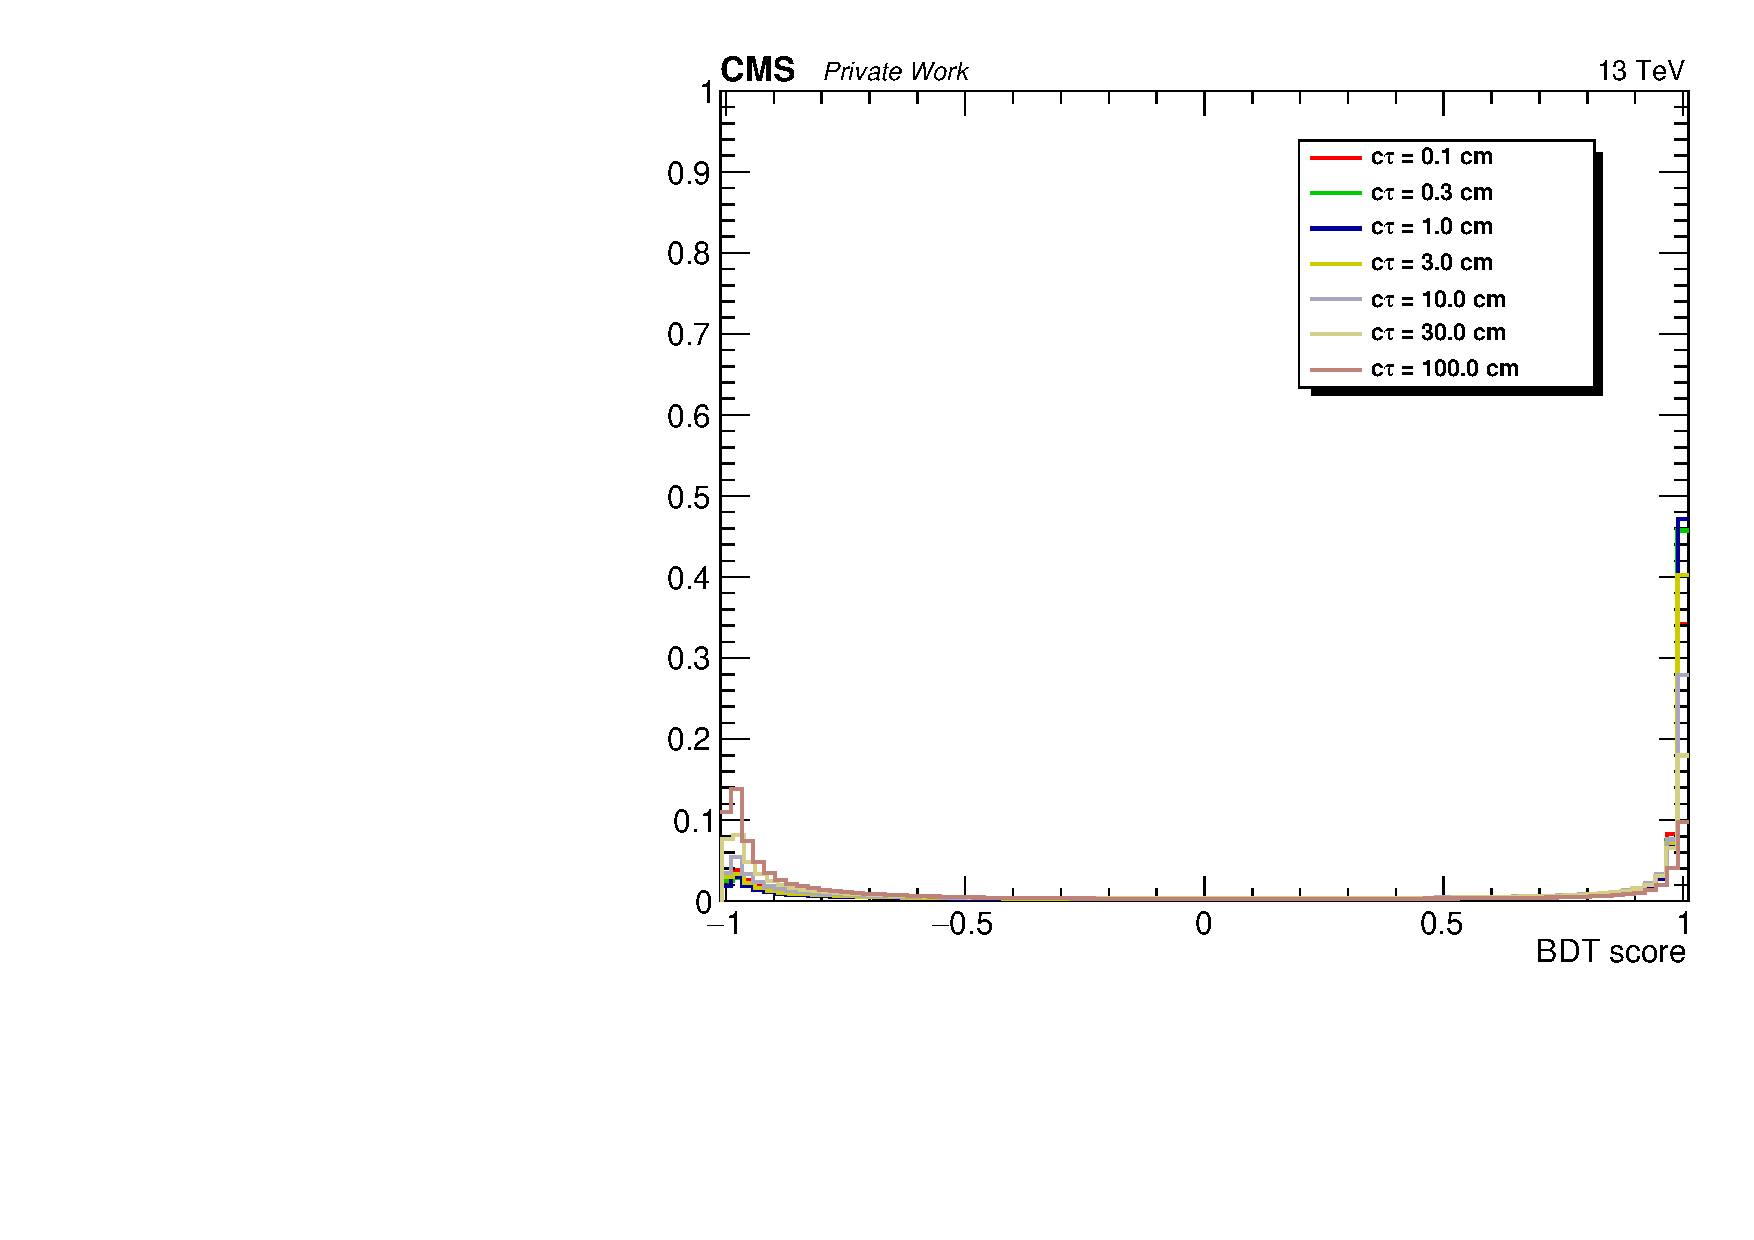
\includegraphics[height=9cm, width=12cm, trim= 0cm 0cm 0cm 0cm,clip]{images/TRKBDT/plot_BDTTRKvsctau.pdf}
\caption{\label{fig:BDTctau} Track BDT score distributions for different neutralino $c\tau$. }
\end{figure}

\FloatBarrier
Since the BDT is trained for a specific neutralino lifetime, the selection efficiency of the track selection BDT can vary as a function of the neutralino decay length. Figure \ref{fig:BDTctau} shows that the best discriminating power is obtained for a $c\tau$ of 1.0 cm and remains good for all decay length except for a $c\tau$ of 100.0 cm. This can be expected as the $\beta\gamma$ of the neutralino is about 2.5, most tracks coming from the neutralino are out of the tracker and the remaining tracks come from the primary vertex, pile-up or fake-tracks.

\subsubsection{Dependence of the track selection BDT with respect to the difference of mass between the neutralino and the smuon}
   \begin{figure}[ht]
\centering
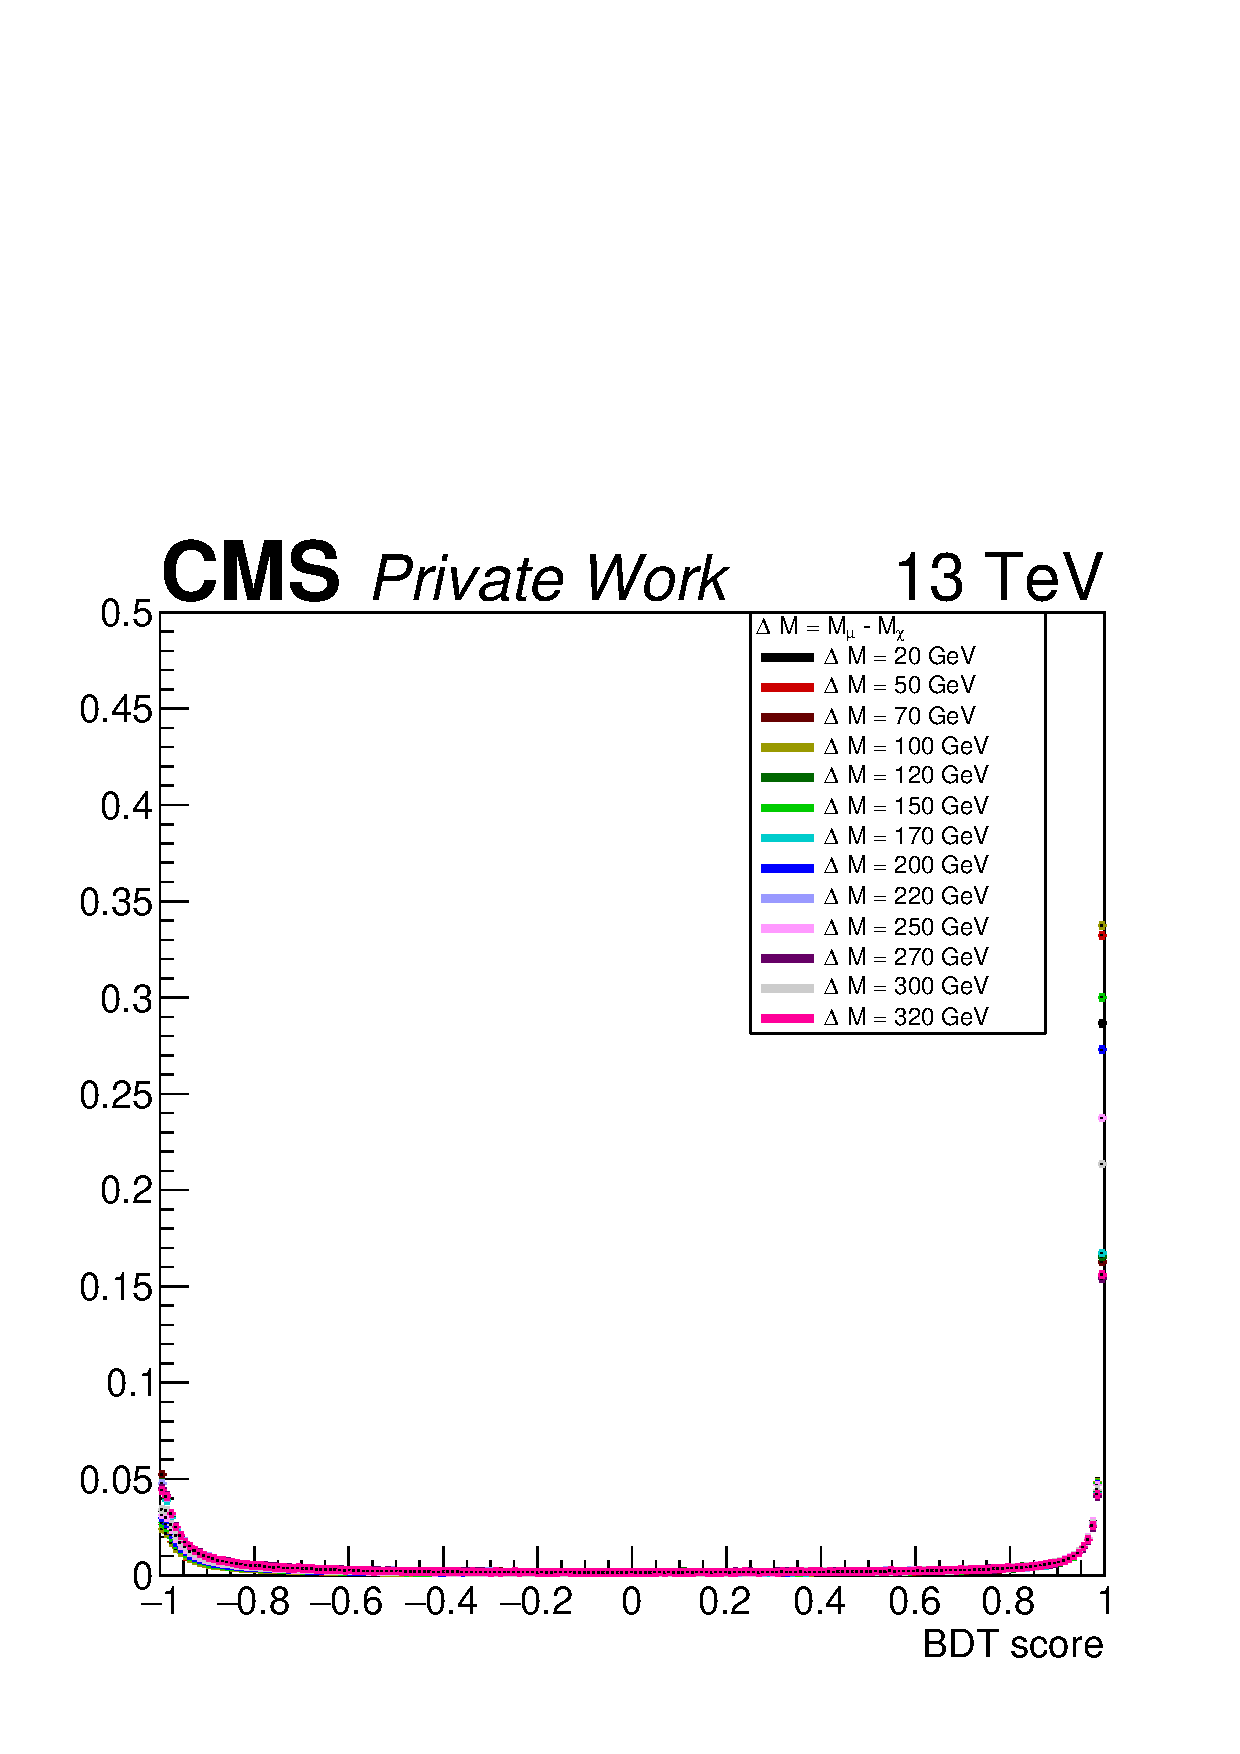
\includegraphics[height=10cm, width=11cm, trim= 0cm 0cm 0cm 0cm,clip]{images/BDT/plotBDTTRK_dm.pdf}
\caption{\label{fig:BDTctau} Track BDT score distributions for different $\Delta M_{\Tilde{\mu}-\Tilde{\chi}^{1}_{0}}$ for a $c\tau$. = 10.0 cm }
\end{figure}

The BDT score distribution as a function of $\Delta M_{\Tilde{\mu}-\Tilde{\chi}^{1}_{0}}$  shows no major discrepancy between the different samples. Sine the BDT is trained for all the $\Delta M_{\Tilde{\mu}-\Tilde{\chi}^{1}_{0}}$ shown, the BDT is therefore behaving as expected from the Appendix.\ref{APP: TRKBDT}.

%%%%%%%%%%%%%%%%%%%%%%%%%%%%%%%%%%%%%%%%%%%%%%%%%%%%%%%%%%%%%%%
%%%%%%%%%%%%%%%%%%%%%%%%%%%%%%%%%%%%%%%%%%%%%%%%%%%%%%%%%%%%%%%
%------------------- SECTION ----------------------------------
%%%%%%%%%%%%%%%%%%%%%%%%%%%%%%%%%%%%%%%%%%%%%%%%%%%%%%%%%%%%%%%
%%%%%%%%%%%%%%%%%%%%%%%%%%%%%%%%%%%%%%%%%%%%%%%%%%%%%%%%%%%%%%%
\newpage
\section{Displaced Vertices Reconstruction}
\label{SEC: DISVTX}
    The main goal of this analysis is the reconstruction of displaced vertices coming from the decay of a long-lived neutralino decaying in the tracker volume. For the vertexing, only one vertex per hemisphere is reconstructed using the Adaptive Vertex Fitter (AVF) \cite{AVF}. The AVF is a more robust iteration of the Kalman Fitter, more efficient with high-track multiplicity vertices allowing to reach good reconstruction efficiencies for our signal. Features from the AVF will also be used later in Section.\ref{SEC: BKGEST} to discriminate signal and background.\\

    The parameters given as an input of the AVF are given in the Table.\ref{tab:AVFPARAMETERS}. After testing different values for the input parameters, no major changes in the final efficiencies were observed therefore the default values from \cite{AVF} and given in the Table.\ref{tab:AVFPARAMETERS} are kept.\\

            \begin{table}[h]
\centering
\begin{tabular}{|c|c|m{10 cm}|}
  \hline
  \rowcolor{lightgray} 
  Parameter & Value & Definition\\
  \hline
        maxshift & 0.0001 & Convergence criterion in centimeter (maximum transverse distance between vertex computed in the previous and the current iterations)\\
        \hline
        maxstep & 30 & Maximum number of iterations to perform\\
        \hline
        maxlpshift & 0.1 & Criterion for the relinearization of the tracks \\
        \hline
        weightthreshold & 0.001 & Minimum track weight for a track to be considered "significant". If fewer than two tracks are significant, an invalid vertex is returned.\\
        \hline
        sigmacut & 5. & Tracks this number of sigma away from the vertex are given a weight of 0.5\\
        \hline
        Tini & 256. & Parameter used to compute the weight of a given track associated to a vertex\\
        \hline
        ratio & 0.25 &  Parameter used to compute the weight of a given track associated to a vertex\\
  \hline
\end{tabular}
    \caption{Input parameters for the Adaptive Vertex Fitter}
    \label{tab:AVFPARAMETERS}
\end{table}

     A first collection of tracks is built for each hemisphere out of the tight WP and a second one using the loose WP. The vertexing will then be performed in 2 steps for each hemisphere for each WP in order to reconstruct one vertex per hemisphere. A detail of the vertexing workflow is given below.
    
    \subsection{Multi-step vertexing}
        In this analysis, one vertex is reconstructed per hemisphere. Further improvement could be potentially obtained by looking for tertiary vertices coming from the b-jets but these jets can be hard to identify since b-tagging does not apply to largely displaced jets (dozens of centimeters) and also due to the decrease in resolution of the vertices.\\

        For each hemisphere, the tracks are ordered by decreasing BDT score. Then, instead of directly giving a set of tracks to the AVF, we only give the first two tracks for which a valid vertex (eventually with a supplementary 0$<\frac{\chi^2_{vtx}}{DoF}<$10 criterion) is reconstructed. Then, we iterate this procedure by adding one track after the other. The tracks that do not allow for the reconstruction of a vertex are removed. In practice, four steps are defined :
    \begin{itemize}
        \item \textcolor{black}{ A selection of tracks using a high BDT score ($>$ TightWP) is used for the IAVF without the $\frac{\chi^2_{vtx}}{DoF}$ criterion.}
        % \vspace{-4.mm}
        \item \textcolor{black}{ Otherwise, the same tracks are used with the IAVF with a $\frac{\chi^2_{vtx}}{DoF}$ criterion in the iterative procedure.}
        % \vspace{-4.mm}
        \item \textcolor{black}{ Otherwise, a selection of tracks using a loose BDT score ($>$ LooseWP) and applying the IAVF without the $\frac{\chi^2_{vtx}}{DoF}$ criterion}
        % \vspace{-4.mm}
        \item  \textcolor{black}{ Otherwise, the same tracks are used with the IAVF with a $\frac{\chi^2_{vtx}}{DoF}$ criterion in the iterative procedure.}
    \end{itemize}

    If the $\frac{\chi^2_{vtx}}{DoF}$ criterion is fulfilled at the end of a step, the vertex reconstruction is  considered successful and no more step is needed. The efficiency of each step is shown in Fig.\ref{fig:StepEffi} .

    \begin{figure}[ht]
\centering
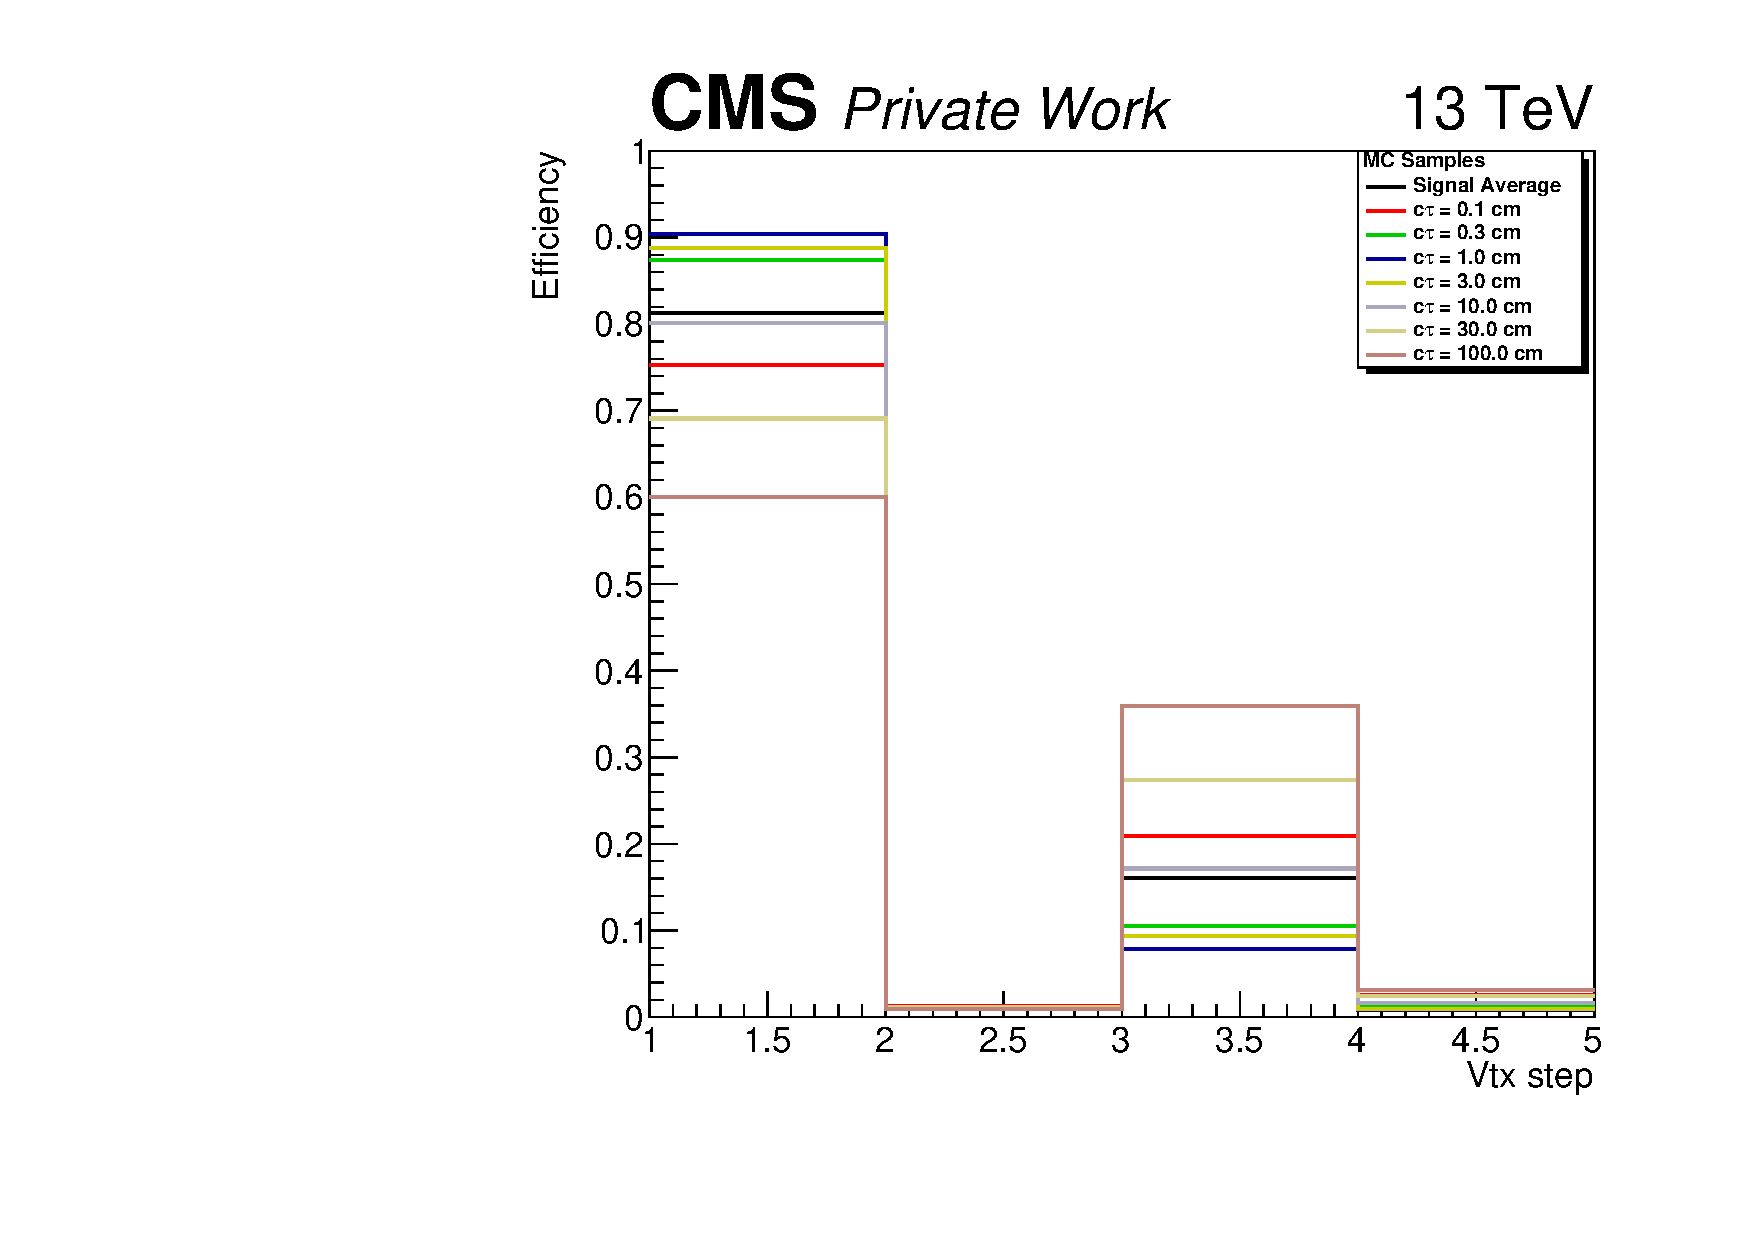
\includegraphics[height=8cm, width=8cm, trim= 0cm 0cm 0cm 0cm,clip]{images/VTXEff/VtxStepEffi_Svsctau.pdf}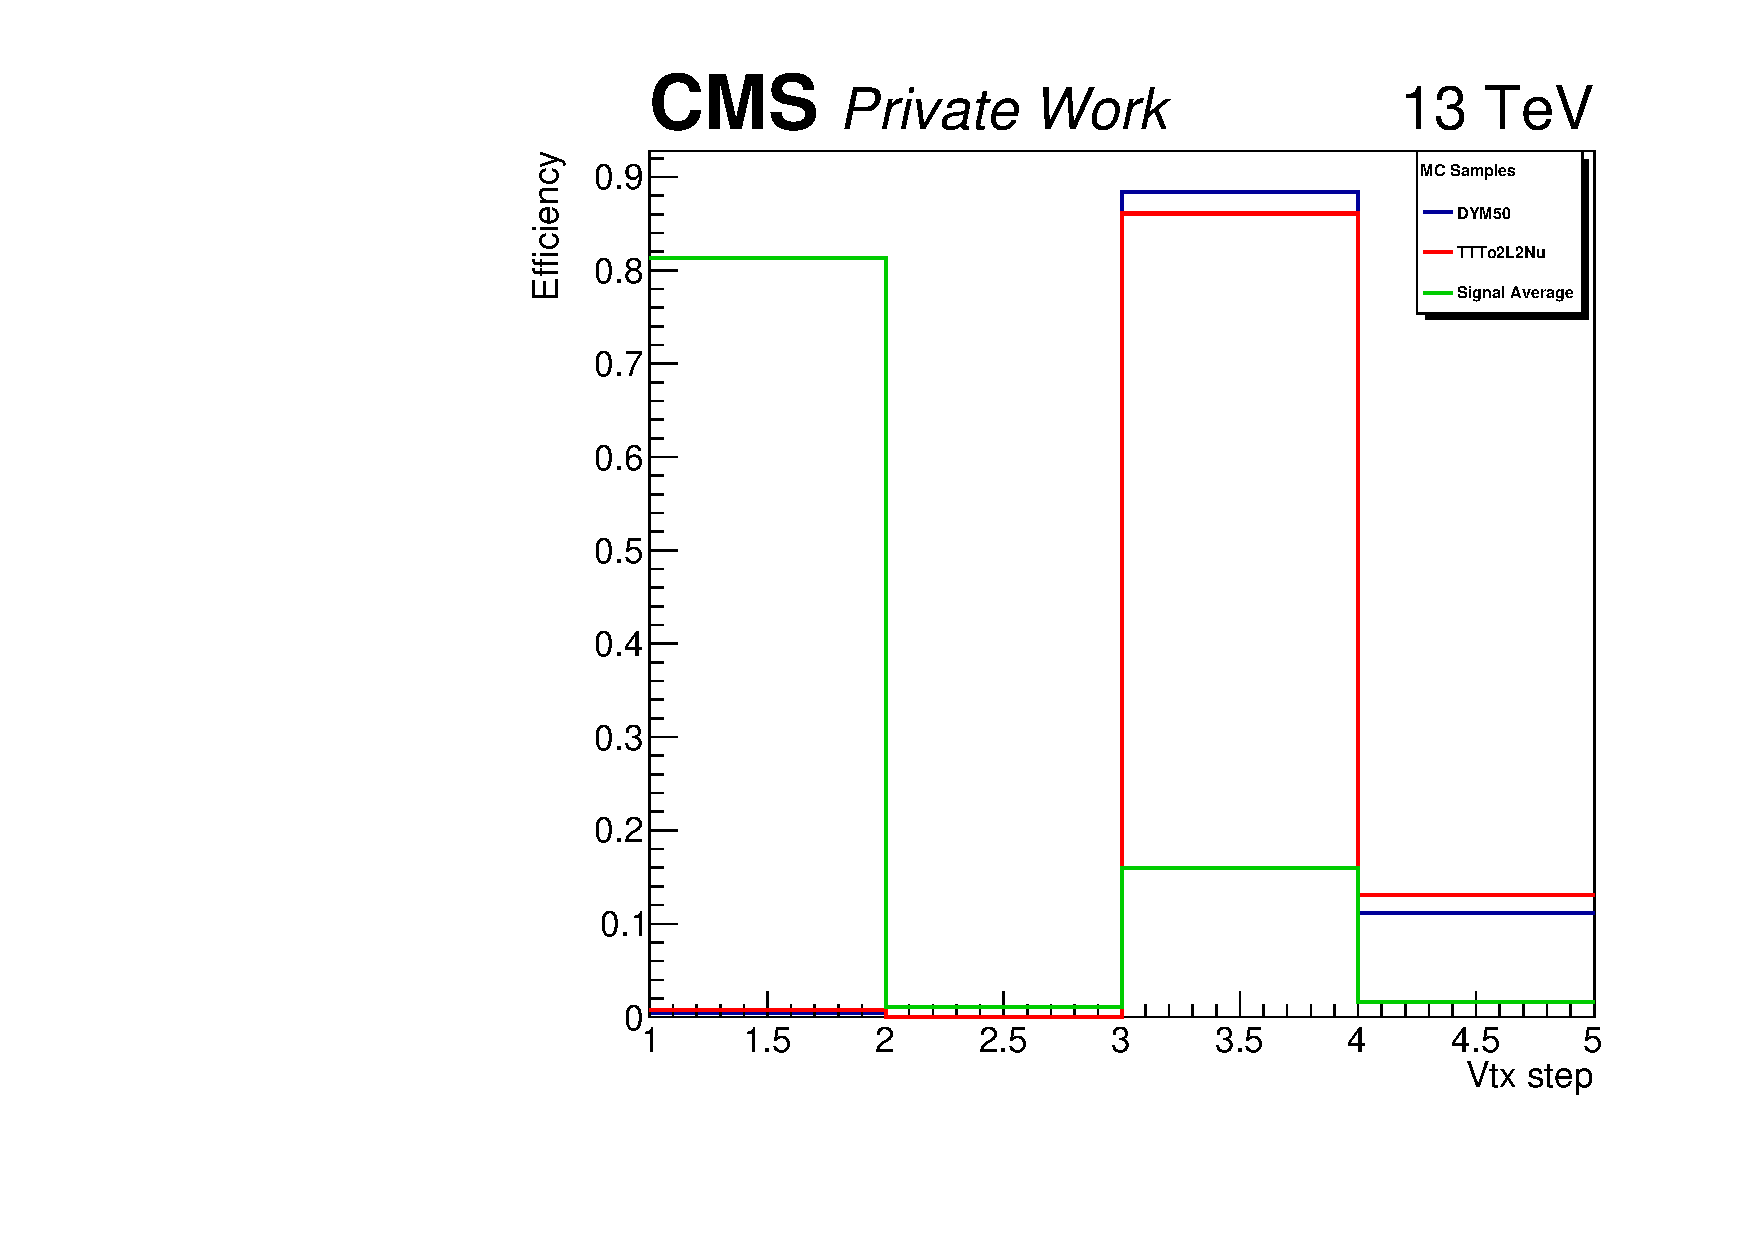
\includegraphics[height=8cm, width=8cm, trim= 0cm 0cm 0cm 0cm,clip]{images/VTXEff/VtxStepEffi_SvsBKG.pdf}
\caption{\label{fig:StepEffi} Step relative contribution to the reconstruction efficiency before merging as a function of the mean neutralino decay (Left) and for two different background samples (Right). }
\end{figure}   

        In this multi-step vertexing, some tracks are removed if they do not respect the criteria that the first hit of any track must come after the position of the vertex that is built or the newly added track does not allow to reconstruct a valid vertex. Out of these removed tracks, there is a possibility that these tracks belong to a tertiary displaced vertices coming from b-jets or real signal vertices. However, applying the AVF on the removed tracks has not shown any improvement in the vertex reconstruction efficiency.
    
    \textcolor{black}{In 10\% to 30\% of the cases, the two reconstructed vertices are too close to each other, below the vertex resolution. Therefore, a merging step is needed by combining the two vertices. The remaining tracks are used to look for another secondary vertex.}\\
    \subsection{Vertex Merging}
        
        The multi-step vertexing has the goal of reconstructing one vertex per hemisphere. Even if the two hemispheres are well reconstructed (opposite in $\phi$ and close to the generated neutralino axis), it happens that two reconstructed vertices are really close in the 3D-space and pointing to the same neutralino meaning the 3-d distance between the two vertices can be below the resolution level. A merging step is implemented as well as a new search of displaced vertex.

        \subsubsection{Merging}
            Since a tight and loose working point are defined for the vertices, one has to be careful when combining the information (mass, number of tracks, $\frac{\chi^2}{dof}$, position, quality) about the two close vertices.
            \begin{itemize}
                \item When both vertices are loose or tight, the mean position between the two original vertices is taken as the new position of the merged vertex. This approximation has been verified to be good since applying the AVF to the collections of tracks of the two original vertices gave a vertex at mean distance between the two original vertices (and both vertices are already close in position $\sim$ 1 mm). The approximation was made in order to gain computing time and avoid the AVF to crash for any reason and lose a vertex. The mass of the new vertex is the sum of the two original masses, the $\frac{\chi^2}{dof}$ is defined as the average $\frac{\chi^2}{dof}$ of the two original vertices and the tracks are just added together to define the new track multiplicity. If the two vertices are tight (loose), the final vertex is defined as tight (loose).
                
                \item When one of the vertex is loose and the other one is tight, the tight vertex is taken as the final vertex with all its associated information  (mass, number of tracks, $\frac{\chi^2}{dof}$, position). The final vertex is defined as tight.
            \end{itemize}
        The definition of the quality tag for merging enables to keep the tight vertices that we expect to be good signal vertices and remove potentially background (signal-like) vertices. However, we lose one vertex by doing this procedure. In order to potentially have 2 vertices in an event that needs merging, a second vertex is searched for. The probability of having to merge two vertices is shown in Fig.\ref{fig:MERGE} on the left plot.
        \begin{figure}[ht]
            % \centering
            \hspace{-1cm}
            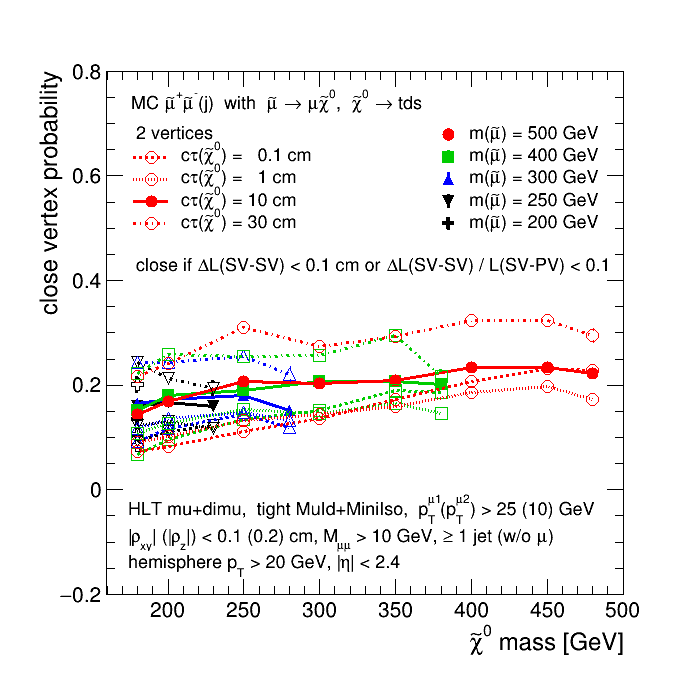
\includegraphics[height=10cm, width=9cm, trim= 0cm 0cm 0cm 0.cm,clip]{images/Merging/close_2vtx_ctau_240322.png}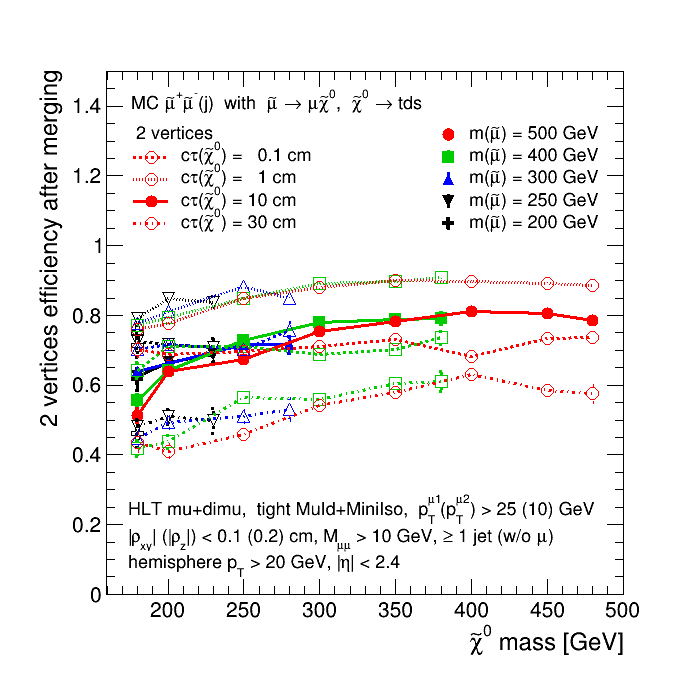
\includegraphics[height=10cm, width=9cm, trim= 0cm 0cm 0cm 0.cm,clip]{images/Merging/merge_2vtx_ctau_240322.png}
            \caption{\label{fig:MERGE} Left plot : Probability of having to merge vertices together. Right plot : probability of reconstructing a new secondary vertex after merging. Figures are shown as function of the neutralino mass for different $c\tau$ of the latter and different masses for the smuon}
        \end{figure}


        
        \subsubsection{Search for a new secondary vertex}
            In order to look for a new secondary vertex, the $\Delta R$ between the two axes and the merged vertex is computed to assign this vertex an hemisphere, the closest one. This allows to look for a new secondary vertex in the other hemisphere. In order to not recompute the same vertex as one of the two original one, the tracks with a weight above 0.05 from the original vertices are removed from the computation of the new secondary vertex ($\Leftrightarrow$ the probability of the track to belong to the original vertex is below 5\%). \\
            The 4 steps of vertexing are then used with the selected tracks of the hemisphere to compute this new vertex. The quality tag is defined as per the original vertices, which again tend to assign tight vertices to the signal and loose to the background vertices. The probability of reconstructing a new secondary vertex after merging is shown in Fig.\ref{fig:MERGE} on the right plot.

    
        
        \subsubsection{Vertex reconstruction efficiency}

                The reconstruction of the signal is expressed as the vertex reconstruction efficiency as a function of the decay length of the neutralino. This efficiency can also be expressed as a function of the transverse distance  or $|\eta|$.
                In this analysis, a vertex is considered reconstructed when the $\frac{\chi^2}{dof}$ is between 0 and 10.  For signal MC samples, a criteria is added on the matching between the reconstructed vertex and the generated one: the relative distance between the two vertices must be lower than 10\% of the generated decay length (called matched vertices). 
                \begin{itemize}
                    \item The efficiency is computed as the ratio between the number of matched vertices by the number of vertices that should be reconstructed in theory, i.e twice the amount of events passing the online+offline selection.
                    \item The second quantity that can be defined in signal MC samples is the purity, that is the ratio between the number of matched vertices and the number of vertices having a $\frac{\chi^2}{dof}$ between 0 and 10.
                \end{itemize}
            Both quantities are shown in Fig.\ref{fig:VTXEff}.  

\begin{figure}
    \centering
    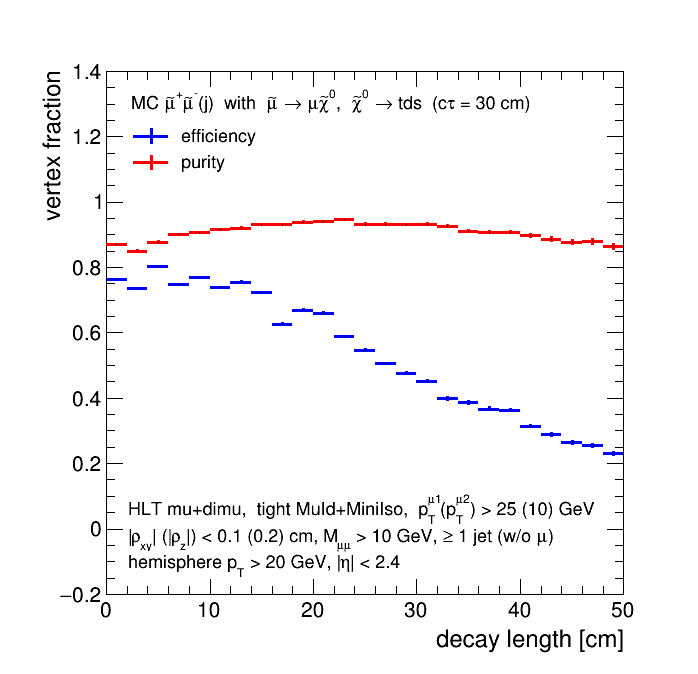
\includegraphics[width=0.5\linewidth]{images/VTXEff/eff_dist_ctau300.png}
    \caption{Vertex reconstruction efficiency (red) and purity (blue) as a function of the decay length of the neutralino.}
    \label{fig:VTXEff}
\end{figure}
\FloatBarrier   
 Concerning the purity, the positive slope at the beginning could be due to the decreasing density of tracks that allows the IAVF to find a good vertex. Then purity is also dependant on the resolution on the vertices for high decay length. The vertex reconstruction efficiency is highly dependant on the tracking efficiency causing the negative slopes after a decay length of 10 cm.

Finally, the vertex reconstruction efficiency is shown as a function of the smuon and neutralino masses in Fig.\ref{fig:VTXEffmass} for a given $c\tau$.
\begin{figure}[ht]
\centering
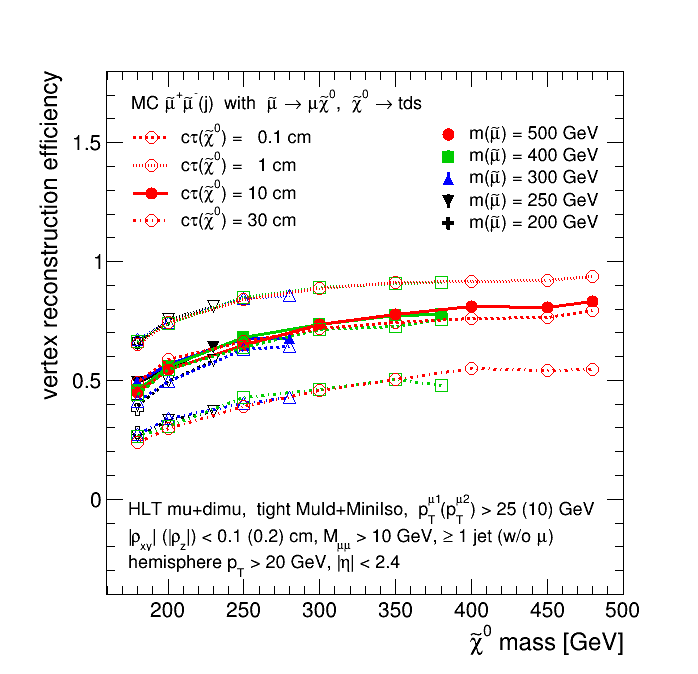
\includegraphics[height=8cm, width=8cm, trim= 0cm 0cm 0cm 0cm,clip]{images/VTXEff/eff_ctau_240328.png}
\caption{\label{fig:VTXEffmass} Vertex reconstruction efficiency as a function of the mass of the neutralino and the smuon.}
\end{figure}   
 In most part of the phase space, the signal event can be identified since in most part of the phase space, one vertex over two is reconstructed.


\FloatBarrier
        \subsubsection{Resolution on the reconstructed vertices}
        The resolution on the position of the vertices is an indicator of the quality of the reconstructed vertices. Since the reconstructed vertices are displaced, the resolution is shown as a function of the decay length in the transverse plane in the barrel region and on the longitudinal axis in the endcaps. The resolution is computed as the distance between a vertex of signal and a vertex of secondary interaction  
        and shown in Fig.\ref{fig:VTXRes}   
        \begin{figure}[ht]
        \hspace{-1cm}
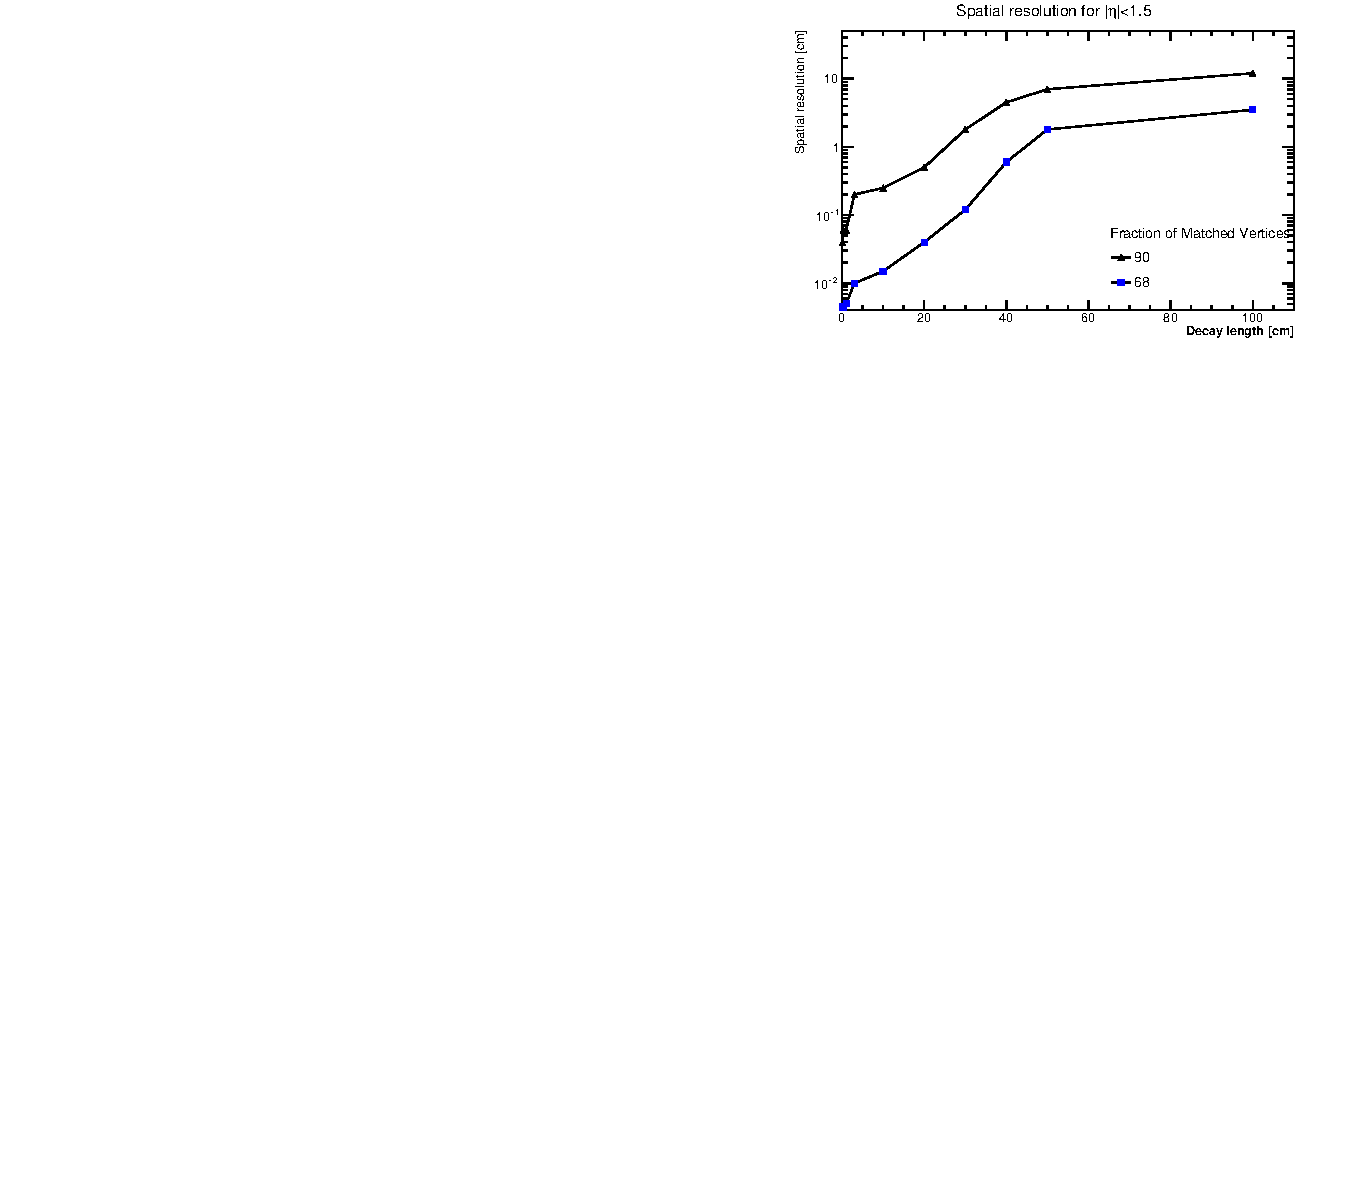
\includegraphics[height=6cm, width=8.5cm, trim= 0cm 7cm 0cm 0cm,clip]{images/VTXRes/ResTrans.pdf}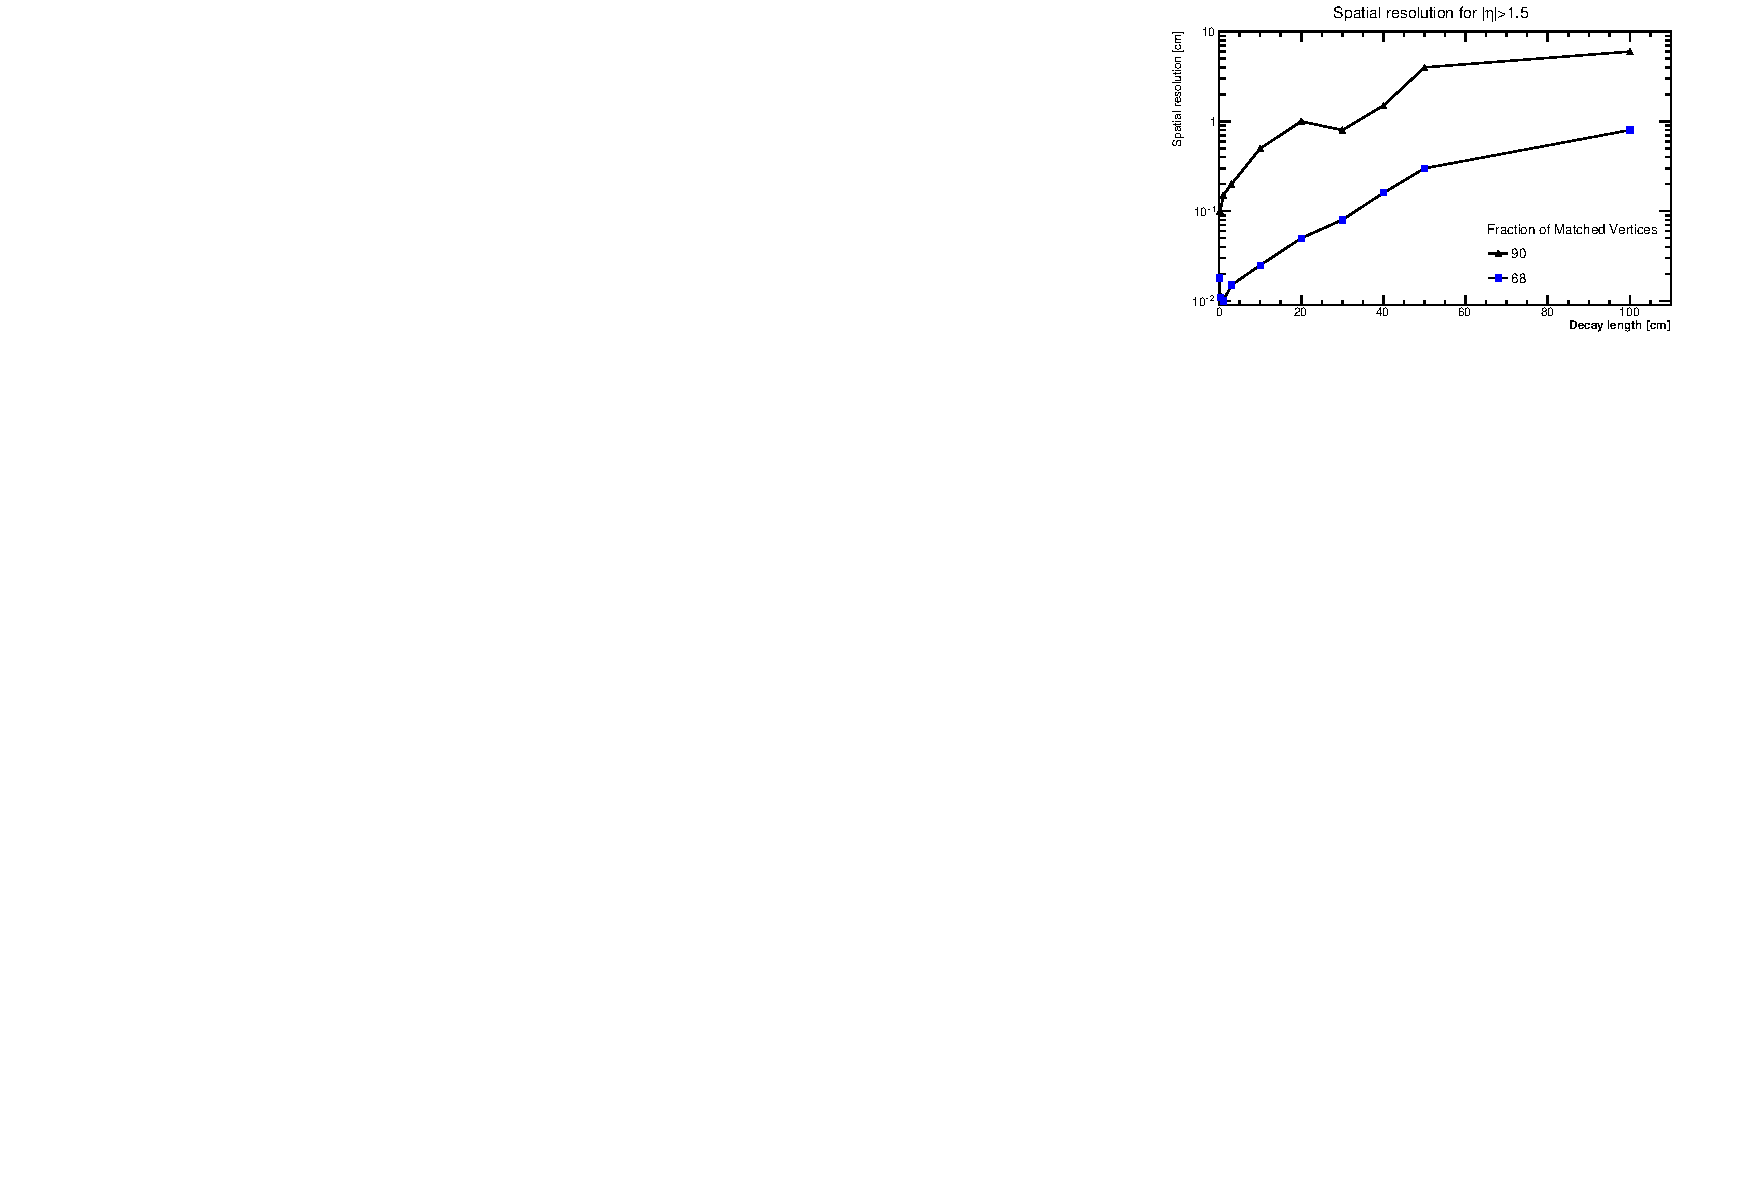
\includegraphics[height=6cm, width=8.5cm, trim= 0cm 0cm 0cm 0cm,clip]{images/VTXRes/ResLong.pdf}
\caption{\label{fig:VTXRes} Transverse (longitudinal) resolution  in the transverse plane (longitudinal axis) as a function of the decay length }
\end{figure}   

%%%%%%%%%%%%%%%%%%%%%%%%%%%%%%%%%%%%%%%%%%%%%%%%%%%%%%%%%%%%%%%
%%%%%%%%%%%%%%%%%%%%%%%%%%%%%%%%%%%%%%%%%%%%%%%%%%%%%%%%%%%%%%%
%------------------- SECTION ----------------------------------
%%%%%%%%%%%%%%%%%%%%%%%%%%%%%%%%%%%%%%%%%%%%%%%%%%%%%%%%%%%%%%%
%%%%%%%%%%%%%%%%%%%%%%%%%%%%%%%%%%%%%%%%%%%%%%%%%%%%%%%%%%%%%%%

\newpage

\section{Event reweighting}
    \label{EVENT_W}
    \subsection{Reweighting from generation}
        The reweighting of the different MC samples is performed at the generator level using \cite{LHEReaderCMSSW}.
    \subsection{PileUp}
        Pile-up distributions tend to be different between data and MC. A pile-up reweighing is therefore needed to make up for the discrepancies. The reweighting procedure is detailed in : \cite{PileupMCReweightingUtilities}.
        
    \subsection{Prefiring}
        A gradual shift of ECAL not propagated to L1 trigger primitives has resulted in a significant fraction of high $\eta$ trigger primitives to be mis-associated to the previous bunch crossing. Since L1 rules do not allow for two consecutive bunch crossing to fire, this can induce some missing event, up to 50\% for jets of several hundreds of GeV for $2.5<|\eta|<3$. The same effect is observed in the muon system due to a limited time resolution in the whole $\eta$ range. Both these effects are simulated and have to be corrected for. The procedure is described in : \cite{L1PrefiringWeightRecipe}
    \subsection{Top $p_{t}$ Reweighting}
            
            Run 1 and Run 2 analyses have shown that the $p_T$ spectra of top quarks in $t\bar{t}$ data was significantly softer than those predicted by different generators. This implies a correction of the reconstructed top $p_T$ based  on the generated $p_T$. Several methods are given by the Top PAG in \cite{TopPtReweighting}. In the case of the search for displaced top quark, the $t\bar{t}$ MC sample is used to probe BSM and to model background. Once the reweighing factor is deduced from a control region enriched in $t\bar{t}$, it can be applied to $t\bar{t}$ MC samples. The Top PAG already provides a function for the reweighing factor as a function of the generated top $p_T$ :

            \begin{equation}
                SF(p_T) = e^{0.0615-0.0005.p^{Gen}_T}
            \end{equation}
%%%%%%%%%%%%%%%%%%%%%%%%%%%%%%%%%%%%%%%%%%%%%%%%%%%%%%%%%%%%%%%
%%%%%%%%%%%%%%%%%%%%%%%%%%%%%%%%%%%%%%%%%%%%%%%%%%%%%%%%%%%%%%%
%------------------- SECTION ----------------------------------
%%%%%%%%%%%%%%%%%%%%%%%%%%%%%%%%%%%%%%%%%%%%%%%%%%%%%%%%%%%%%%%
%%%%%%%%%%%%%%%%%%%%%%%%%%%%%%%%%%%%%%%%%%%%%%%%%%%%%%%%%%%%%%%
\newpage
\section{Background Estimation}
\label{SEC: BKGEST}
 In the signal region defined for this analysis (detailed in the subsection.\ref{ABCD}), the statistics for the different MC samples (DY and $t\Tilde{t}$ especially) are low. The choice is then made to use a data-driven method to better estimate the background in this signal region.
    \subsection{ABCD Method}
        \label{ABCD}
        The multiple selections and observables in this analysis allow to combine them to better distinguish signal and background and define background enriched regions (CR for control regions and VR for validation regions) and signal-enriched regions (SR). The heavy hadronic final state can be used to distinguish the signal from backgrounds when comparing the $p_T$ of the two hemispheres introduced in section.\ref{SEC: EVTREC}. The other variable used to distinguish signal from background is the working point (Tight or Loose) from the track selection BDT that was used to build the vertex. Different ABCD comparisons will be shown depending on the number of reconstructed vertices (1 or 2) while looking at the distributions of the sum of the weights of the tracks associated to a vertex (this variable is described in section.\ref{SEC: SUM}). Another potential distribution is the mass of the reconstructed vertices and will be shown in Appendix.\ref{APP:ABCDVTXMASS}. The ABCD method can then be defined as shown in Fig.\ref{fig:ABCD_sch}.
        \begin{figure}[ht]
\centering
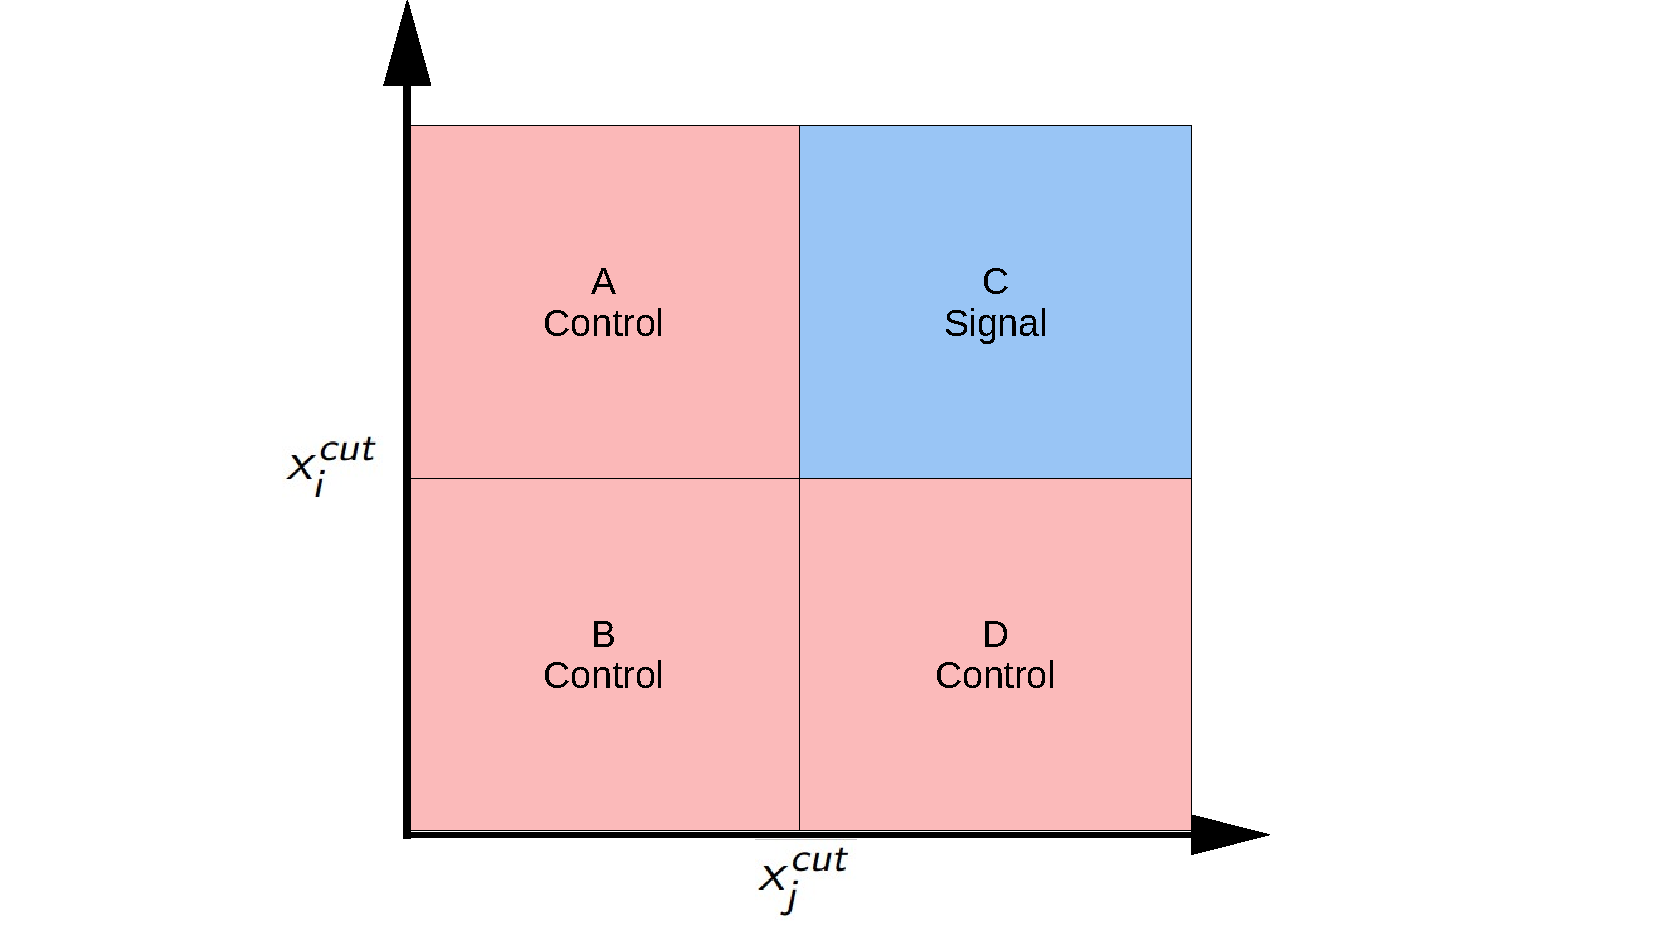
\includegraphics[height=10cm, width=17cm, trim= 0cm 0cm 0cm 0cm,clip]{images/ABCD/ABCD.pdf}
\caption{\label{fig:ABCD_sch} The background estimation method shown with three control regions and 1 signal region. The regions are defined using two cut on non-correlated variables $x_{i}^{cut}$ and $x_{j}^{cut}$. In all four regions, one discriminating variable between signal and background is used to observe the signal in region C. The three other regions are used to predict the background in the signal region which is blinded from data.}
\end{figure}  
\FloatBarrier
        The signal region is defined as the region C where the background is estimated as follows :
        \begin{equation}
             N_{C}^{BKG} = \frac{N_{A}^{BKG}*N_{D}^{BKG}}{N_{B}^{BKG}}
        \end{equation} where $N_{X}^{BKG}$ is the number of background events in the region X.

        \begin{figure}[ht]
\centering
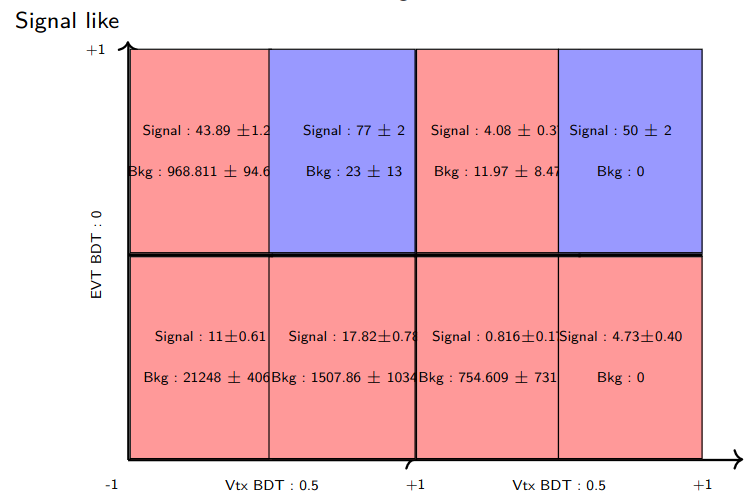
\includegraphics[height=8cm, width=12cm, trim= 0cm 0cm 0cm 0cm,clip]{images/ABCD/EVTYieldsRun2.png}
\caption{\label{fig:EVTYIELDS} Event yields for Run 2 for the one vertex and two vertices categories. The two categories are defined as : "Exactly one vertex reconstructed" and "Exactly two vertices reconstructed" where a vertex is considered reconstructed when its follows $0<\frac{\chi^2}{DoF}<10$. For signal samples, the reconstructed vertex is required to be within 10\% matching with the generated vertex such that : the difference in position between the reconstructed and generated vertices is below 10\% of the generated vertices decay length. The signal region is defined by a BDT value above 0 for the event selection BDT and above 0.5 for the vertex selection BDT. }
\end{figure}  
\FloatBarrier
        \subsection{Validations}
        In order to validate ABCD method, the workflow is tested on the $e\mu$ data and MC samples with specific selections (triggers, dilepton mass, lepton IDs and ISOs, MET) for this channel that are defined in Appendix.\ref{APP: VALIDEMU}. Results are shown in Fig. for the 1 vertex category and in Fig. for the 2 vertex category.
        Correlations between the hemisphere $p_T$ and the use of the two working points are shown in Fig. .
        Signal contamination plots are shown in Fig. for the 1 vertex category and in Fig. in the 2 vertex category \textcolor{red}{add plots}
        \textcolor{red}{Plot is outdated,}
   
    \newpage
%%%%%%%%%%%%%%%%%%%%%%%%%%%%%%%%%%%%%%%%%%%%%%%%%%%%%%%%%%%%%%%
%%%%%%%%%%%%%%%%%%%%%%%%%%%%%%%%%%%%%%%%%%%%%%%%%%%%%%%%%%%%%%%
%------------------- SECTION ----------------------------------
%%%%%%%%%%%%%%%%%%%%%%%%%%%%%%%%%%%%%%%%%%%%%%%%%%%%%%%%%%%%%%%
%%%%%%%%%%%%%%%%%%%%%%%%%%%%%%%%%%%%%%%%%%%%%%%%%%%%%%%%%%%%%%%
\section{Control region for $t\Bar{t}$ $\rightarrow$ e$\mu$ + jets}
\label{APP: VALIDEMU}
For signal region, the dominate background is $t\Bar{t}$ which is estimated by reconstructing control region by selecting e$\mu$ + jets. 
\subsection{Data and Monte Carlo Samples}\label{sec:samples}
%Below is a summary of the data and simulation samples used in this analysis. This analysis has been done using CMSSW$\_$10$\_$6$\_$30 software release for the 2016, 2017, and 2018 data-taking periods, respectively.
The data samples used in this analysis were collected by the CMS experiment during 2016, 2017, and 2018 data-taking periods which corresponds to an integrated luminosity of 36.30 fb$^{-1}$, 41.47 fb$^{-1}$, and 59.80 fb$^{-1}$ are listed in Tables~\ref{tab:datasets2016},~\ref{tab:datasets2017}, and~\ref{tab:datasets2018} respectively. For this analysis, the data is triggered with single or double muon and electron high level triggers (HLTs), with 25$\sim$ns bunch crossing for 2016--2018 data-taking periods. The different statistics corresponding to the different periods of data taking, corresponding to different technical conditions of the machine.

%For each dataset,  the set of trigger that are used is given in Table \ref{tab:TRIGGER2016} for 2016, in Table \ref{tab:TRIGGER2017} for 2017 and in Table\ref{tab:TRIGGER2018} for 2018.

\begin{table}[h]\label{tab:datasets2016}
\begin{center}

\begin{tabular}{|l|l|}
\hline     
Dataset(pp collision 2016) & $\cal L$ (\fbinv)  \\\hline
/MuonEG/Run2016B-ver2\_HIPM\_UL2016\_MiniAODv2-v2/MINIAOD     & 5.82  \\
/MuonEG/Run2016C-HIPM\_UL2016\_MiniAODv2-v2/MINIAOD      & 2.60 \\
/MuonEG/Run2016D-HIPM\_UL2016\_MiniAODv2-v2/MINIAOD   & 4.28 \\
/MuonEG/Run2016E-HIPM\_UL2016\_MiniAODv2-v2/MINIAOD     & 4.06 \\
/MuonEG/Run2016F-HIPM\_UL2016\_MiniAODv2-v2/MINIAOD    & 2.72 \\
/MuonEG/Run2016F-UL2016\_MiniAODv2-v2/MINIAOD    & 0.42 \\
/MuonEG/Run2016G-UL2016\_MiniAODv2-v2/MINIAOD     & 7.65 \\
/MuonEG/Run2016H-UL2016\_MiniAODv2-v2/MINIAOD      & 8.73    \\\hline
Total Lumi & 36.30 \\ \hline
\end{tabular}
\end{center}
\caption{List of 2016 MuonEG data samples and the approximate luminosity as measured using \tt brilcalc with the JSON file $${\tt Cert\_271036-284044\_13TeV\_Legacy2016\_Collisions16\_JSON.txt }$$ in location /afs/cern.ch/cms/CAF/CMSCOMM/COMM$\_$DQM/certification/Collisions16 \\/13TeV/Legacy\_2016/ .}\label{tab:datasets2016}
\end{table}
\begin{table}[htbp]\label{tab:datasets2017}
\begin{center}
\begin{tabular}{|l|l|}
\hline
Dataset(pp collision 2017) & $\cal L$ (\fbinv) \\\hline
/MuonEG/Run2017B-UL2017\_MiniAODv2-v1/MINIAOD    & 4.80 \\
 /MuonEG/Run2017C-UL2017\_MiniAODv2-v1/MINIAOD  & 9.57 \\
/MuonEG/Run2017D-UL2017\_MiniAODv2-v1/MINIAOD   & 4.25 \\
 /MuonEG/Run2017E-UL2017\_MiniAODv2-v1/MINIAOD      & 9.31 \\
 /MuonEG/Run2017F-UL2017\_MiniAODv2-v1/MINIAOD      & 13.54 \\ \hline
 Total Lumi & 41.48 \\ \hline
 \end{tabular}
\end{center}
\caption{List of 2017 MuonEG data samples and the approximate luminosity as measured using \tt brilcalc with the JSON file $${\tt Cert\_294927-306462\_13TeV\_UL2017\_Collisions17\_GoldenJSON.txt}$$ in location afs/cern.ch/cms/CAF/certification/Collisions17/13TeV/Legacy\_2017/ .}\label{tab:datasets2017}
\end{table}
\begin{table}[htbp]\label{tab:datasets2018}
\begin{center}
\begin{tabular}{|l|l|}
\hline
Dataset(pp collision 2018) & $\cal L$ (\fbinv) \\\hline
 /MuonEG/Run2018A-UL2018\_MiniAODv2\_GT36-v1/MINIAOD      &  11.41 \\
 /MuonEG/Run2018B-UL2018\_MiniAODv2\_GT36-v1/MINIAOD    & 7.06 \\
  /MuonEG/Run2018C-UL2018\_MiniAODv2\_GT36-v1/MINIAOD     & 6.89  \\
  /MuonEG/Run2018D-UL2018\_MiniAODv2\_GT36-v1/MINIAOD     & 30.02 \\ \hline
Total  & 59.80 \\ \hline
\end{tabular}
\end{center}
\caption{List of 2018 MuonEG data samples and the approximate luminosity as measured using \tt brilcalc with the JSON file $${\tt Cert\_314472-325175\_13TeV\_Legacy2018\_Collisions18\_JSON.txt}$$ in location afs/cern.ch/cms/CAF/CMSCOMM/COMM$\_$DQM/certification/Collisions18/13TeV \\/Legacy\_2018/.}\label{tab:datasets2018}
\end{table}
\subsection{Simulation}\label{sec:samples}
 MC samples used in this analysis for full Run 2 is same as mentioned in Section 2.2. 
 %The MC samples are processed with the full CMS detector simulation based on \GEANTfour~\cite{Agostinelli:2002hh}. The simulated events are reconstructed using the same algorithms as used for the data and include additional interactions per bunch crossings, referred to as pileup (PU). Simulated events are weighted so that the PU distribution reproduces the one observed in data, which has an average of about 23 (32) interactions per bunch crossing in 2016 (2017 and 2018).


\subsection{Trigger}
The Single and double lepton triggers, as listed in Table ~\ref{tab:trigger}, are used in the present analysis. Single muon triggers have p$_{T}$ thresholds of 24, 27, and 24 GeV for different data takings 2016, 2017, and 2018 respectively. While, thresholds for single electron triggers are 27, 35, and 32 GeV for data collected during 2016, 2017, and 2018. 
The dilepton trigger have p$_{T}$ thresholds of 8 and 23 for muon and 12 and 23 for electrons, respectively for all years.

\begin{table}[htbp]
\begin{center}
\caption{Triggers used to collect events from a given sample for 2016, 2017, and 2018}\label{tab:trigger}
\begin{tabular}{|l|l|l|}
\hline
Year  & Era and MC & Trigger name  \\ \hline
2016 & B-G, MC &  HLT\_Mu8\_TrkIsoVVL\_Ele23\_CaloIdL\_TrackIdL\_IsoVL\_v$\star$ $||$\\

& & HLT\_Mu23\_TrkIsoVVL\_Ele12\_CaloIdL\_TrackIdL\_IsoVL\_v$\star$ \\
 & & $||$ HLT\_Ele27\_WPTight\_Gsf\_v$\star$ $||$ HLT\_IsoMu24\_v$\star$ $||$ 
 HLT\_IsoTkMu24\_v$\star$ \\
&  data-H & HLT\_Mu8\_TrkIsoVVL\_Ele23\_CaloIdL\_TrackIdL\_IsoVL\_DZ\_v$\star$ \\
& & $||$ HLT\_Mu23\_TrkIsoVVL\_Ele12\_CaloIdL\_TrackIdL\_IsoVL\_DZ\_v$\star$ $||$ \\ 
&& HLT\_Ele27\_WPTight\_Gsf\_v$\star$ $||$ HLT\_IsoMu24\_v$\star$ $||$ HLT\_IsoTkMu24\_v$\star$ \\ \hline

2017 & B-F, MC & HLT\_Mu8\_TrkIsoVVL\_Ele23\_CaloIdL\_TrackIdL\_IsoVL\_DZ\_v$\star$ $||$ \\
& & HLT\_Mu23\_TrkIsoVVL\_Ele12\_CaloIdL\_TrackIdL\_IsoVL\_DZ\_v$\star$ $||$ \\
&& HLT\_Ele35\_WPTight\_Gsf\_v$\star$ $||$ HLT\_IsoMu27\_v$\star$ \\
\hline

2018 & A-D, MC & HLT\_Mu8\_TrkIsoVVL\_Ele23\_CaloIdL\_TrackIdL\_IsoVL\_DZ\_v$\star$ $||$ \\
&& HLT\_Mu23\_TrkIsoVVL\_Ele12\_CaloIdL\_TrackIdL\_IsoVL\_v$\star$ $||$ \\
&& HLT\_IsoMu24\_v$\star$ $||$ HLT\_Ele32\_WPTight\_Gsf\_v$\star$ \\ \hline

\hline
\end{tabular}
\end{center}
\end{table}


Table~\ref{tab:selection} summarizes the selection criteria used in this analysis.

\begin{table}[htp]%d
\begin{center}
 \begin{tabular}{|c|c|c|c|} \hline

        Object or event    &   Selection \\ \hline
             Muon & $p^{\mu}_{t}>$25 (leading) ~\GeV, $|\eta_\mu|<2.4$,\\
              &  tight ID, pfRelIso0.4 $<$0.15 \\ \hline
     Electron & $p^{e}_{t}>$14 (leading)~\GeV, $|\eta_e|<2.4$,\\
              &  $|\eta_{SC}| < 1.4442$ or $|\eta_{SC}| > 1.556 $, cut-based tight WP ID, \\ \hline
             % & Barrel$\rightarrow$ d0 (dz) 0.05 (0.10), Endcap$\rightarrow$ d0 (dz) 0.10 (0.20) \\ \hline
    Dilepton    &  Two oppositely charged leptons and each leading (subleading) \\
               &               lepton \pt$>$25 (15)~\GeV,$|m_{ll}|>20~\GeV$ \\ \hline
    jets & {tight jet id with lepton veto, \pt$_{jets}>$20~\GeV, $|\eta_{jets}|<2.4$} \\ \hline
    %PU MVA $>$ 0.61($p_{T} <$ 50 GeV)\\ \hline
     % \cPqb-tagged jets &  2016  :   deep CSV tight WP ($>$ 0.8953) \\
      %          &  2017   :   deep CSV tight WP ($>$ 0.8001) \\
       %         &  2018   :   deep CSV tight WP ($>$ 0.7527) \\ \hline
    $E_T^{miss}$ &   $E_{T}^{miss}$ $>$ 40~\GeV  \\ \hline
 \end{tabular}
\end{center}
\caption{Summary of event selection criteria for the dilepton system in the dimuon and the dielectron channels.}
\label{tab:selection}
\end{table}


\section{Validation at detector level}\label{sec:DatavsMC}
Firstly, the data and MC is validated with the inclusive lepton and dilepton selection without any requirement related to jets. Table~\ref{tab:eventyieldfullRun2_incl} reports the event yields for data, signal MC, and different background processes for 2016, 2017, 2018. 
%It is clear from this table that, a background free data sample of Z boson candidates is achieved with the above selection criteria. The simulation predictions are nicely describing the yield in data within 5\%. Figures~\ref{fig:lepZ_fullRun2_ee} and~\ref{fig:lepZ_fullRun2_mumu} show the comparison of data and MC predictions of the standard kinematic variables for the inclusive Z boson events in the electron and the muon channels for full Run 2, respectively.
%For individual runs, similar distributions are shown in Figs.~\ref{fig:leadsubleadele},~\ref{fig:diele},~\ref{fig:ledsubmuon}, and~\ref{fig:dimuon} in Appendix~\ref{sec:Append 2}. There is good agreement of data and simulation within 5\% across the year.\\
%The selected events have $\approx$ 17--18\% background contamination with major contribution arises from the \zcjs, $t\bar{t}$, and \zljs processes which are $\approx$ 6--7\%, $\approx$ 6--7\%, and $\approx$ 3--5\%, respectively.
%Figures~\ref{fig:z1bjet_fullRun2_ee} and~\ref{fig:z1bjet_fullRun2_mumu} reports the data and MC predictions comparison for the electron and the muon channels, respectively, for full Run 2. The similar comparison plots for individual 2016, 2017, and 2018 years are shown in Figs.~\ref{fig:bjetpt_without_corr_factor_ee},~\ref{fig:bjetpt_delta_without_corr_factor_ee},~\ref{fig:bjetpt_without_corr_factor_mumu}, and~\ref{fig:bjetpt_delta_without_corr_factor_mumu} in Appendix~\ref{sec:Append 2}.
%With this selection criteria \zgtoneb, MC predictions overestimate the data up to 10--15\% for 2016 and 2018.

%Data and MC validation is similar in the electron and the muon channels but there is some difference across the years which can be due to difference in tagging conditions.\rowcolor{lightgray} 
% Another reason can be the PDF and tune used in the MC which is the same in 2017 and 2018 but different than for 2016.

\begin{table}[htp]%d
  \caption{Summary of event yields after dilepton selection in $e\mu$ channel for 2016, 2017, and 2018.}
\begin{center}
 \begin{tabular}{|c|c|c|c|} \hline
                  &  2016       &2017         &2018 \\
                  & $e\mu$    & $e\mu$     &  $e\mu$\\\hline
Data             & 219831         & 286875       & 392714 \\\hline
 $t\bar{t}$     & 188496         &  224584      & 323516  \\ \hline
non-$t\bar{t}$ background & 43256   &  58974    & 82684 \\ \hline
Data/MC           &0.95     & 1.01   &0.97  \\ \hline
Purity ($\%$)       & 80       &   79     &  79   \\ \hline
Scale Factor       & 0.94      & 1.01      & 0.96 \\\hline
%Total simulation/Data & 1.01  &               &   \\ \hline
\end{tabular}
\end{center}
\label{tab:eventyieldfullRun2_incl}
\end{table}



\begin{figure}[h]
\centering
 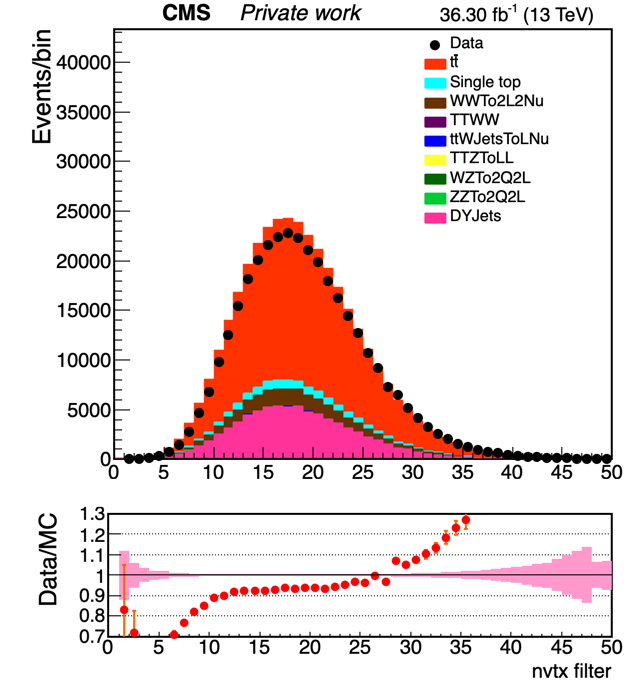
\includegraphics[width=0.32\textwidth]{images/emu_channel/2016/16_Range_0pt7_1pt3/Vertices_filtercut__Linear.png}
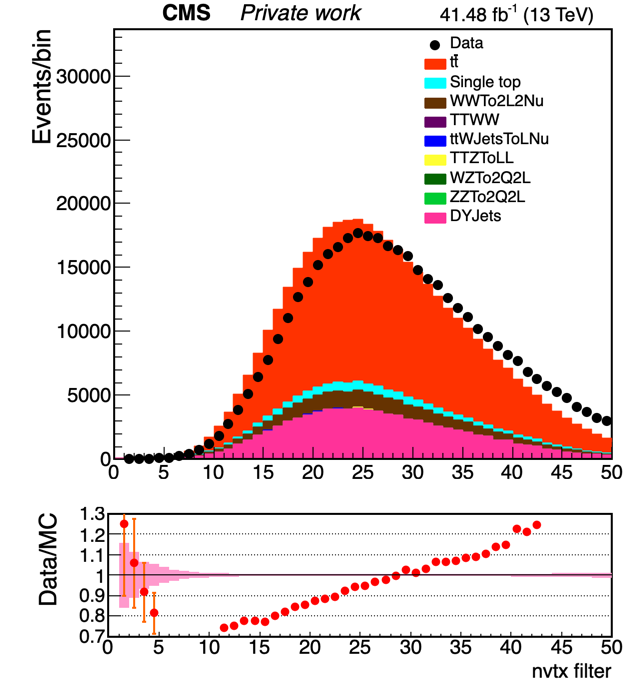
\includegraphics[width=0.32\textwidth]{images/emu_channel/2017/17_Range_0pt7_1pt3/Vertices_filtercut__Linear.png}
 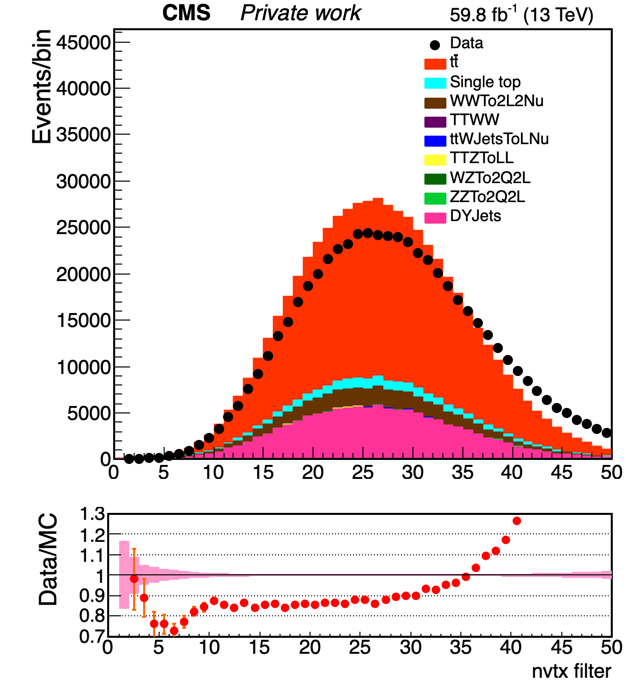
\includegraphics[width=0.32\textwidth]{images/emu_channel/2018/18_Range_0pt7_1pt3/Vertices_filtercut__Linear.png}
  \caption{Distributions of no of primary vertices for 2016 (left), 2017 (middle), 2018(right) Ratio plot at the bottom represents the ratio of data over total MC simulated events.}
%  \caption{Distributions of $\pt$, $|\eta|$, $\phi$ of leading $\mu$ (top) and subleading $\mu$ (middle) and $\mu\mu$ $\pt$, invariant mass, rapidity (bottom) for full Run 2. Ratio plot at the bottom represents the ratio of data over total MC simulated events.}
 \label{fig:nvert_emu}
  \end{figure}
  \begin{figure}[htp]
\centering
 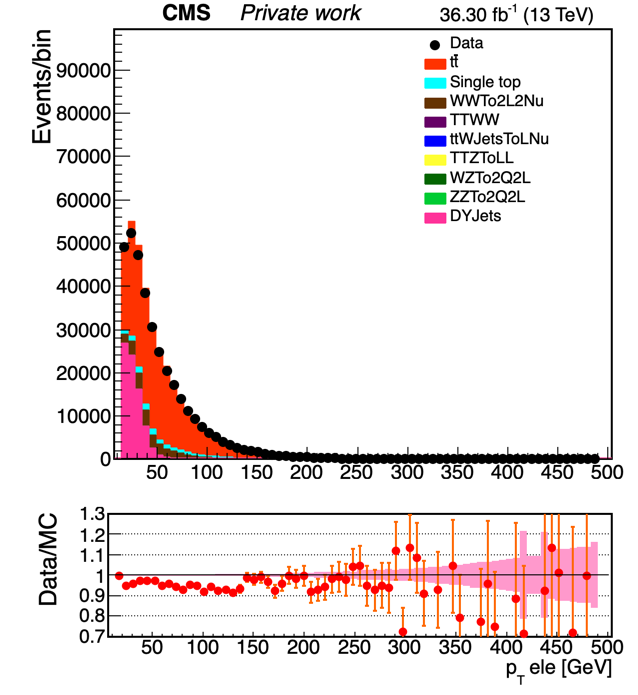
\includegraphics[width=0.32\textwidth]{images/emu_channel/2016/16_Range_0pt7_1pt3/subleading_electron_pt_trig_Linear.png}
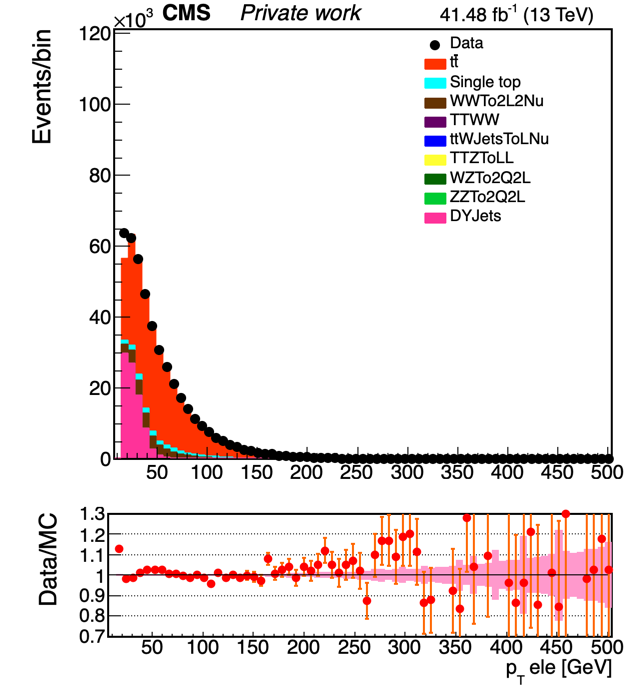
\includegraphics[width=0.32\textwidth]{images/emu_channel/2017/17_Range_0pt7_1pt3/subleading_electron_pt_trig_Linear.png}
 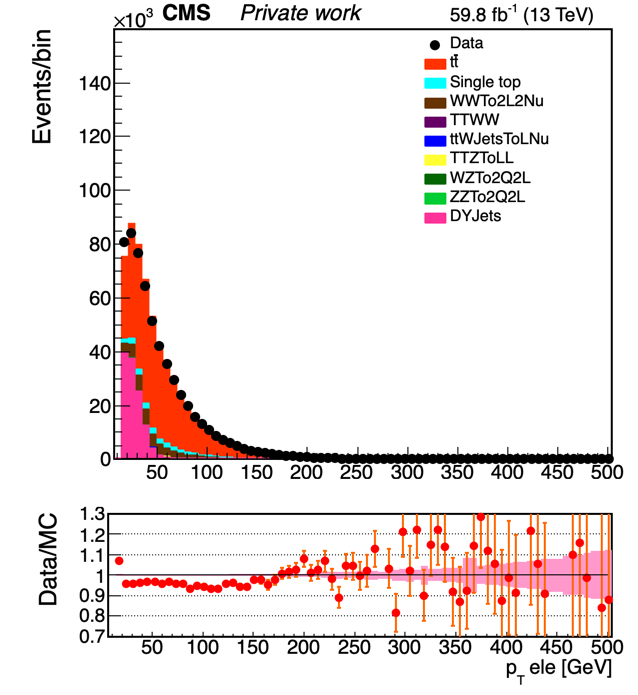
\includegraphics[width=0.32\textwidth]{images/emu_channel/2018/18_Range_0pt7_1pt3/subleading_electron_pt_trig_Linear.png}\\
 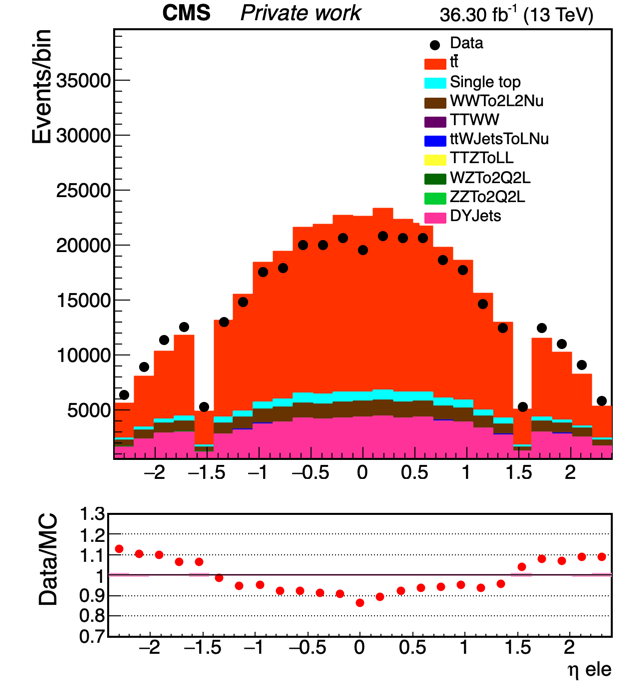
\includegraphics[width=0.32\textwidth]{images/emu_channel/2016/16_Range_0pt7_1pt3/subleading_electron_eta_trig_Linear.png}
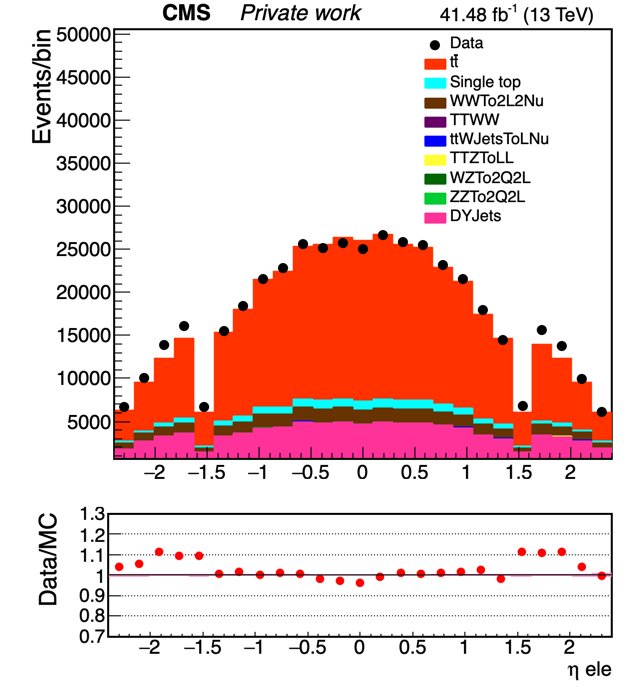
\includegraphics[width=0.32\textwidth]{images/emu_channel/2017/17_Range_0pt7_1pt3/subleading_electron_eta_trig_Linear.png}
 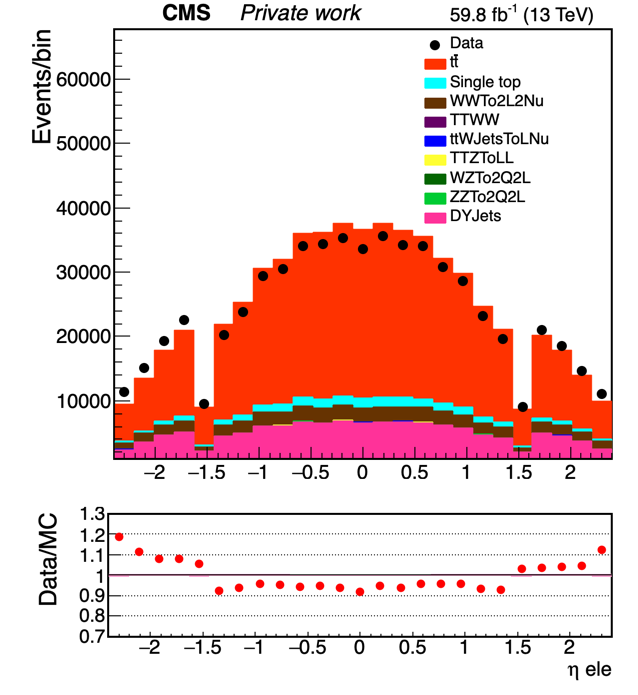
\includegraphics[width=0.32\textwidth]{images/emu_channel/2018/18_Range_0pt7_1pt3/subleading_electron_eta_trig_Linear.png}\\
 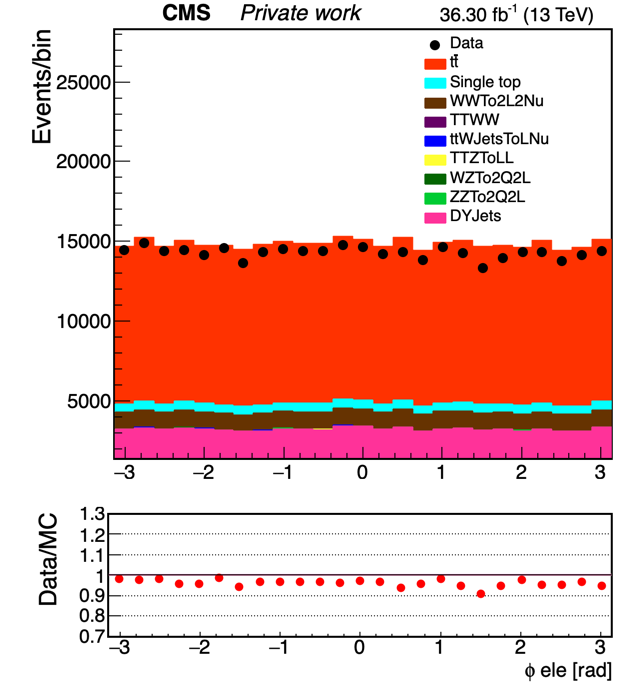
\includegraphics[width=0.32\textwidth]{images/emu_channel/2016/16_Range_0pt7_1pt3/subleading_electron_phi_trig_Linear.png}
\includegraphics[width=0.32\textwidth]{images/emu_channel/2017/17_Range_0pt7_1pt3/subleading_electron_phi_trig_Linear.png}
 \includegraphics[width=0.32\textwidth]{images/emu_channel/2018/18_Range_0pt7_1pt3/subleading_electron_phi_trig_Linear.png} 
 \caption{Distributions of $p_{T}$ (top), $\eta$ (middle), $\phi$ (bottom) of leading electron for 2016 (left), 2017 (middle), 2018(right). Ratio plot at the bottom represents the ratio of data over total MC simulated events.}
%  \caption{Distributions of $\pt$, $|\eta|$, $\phi$ of leading $\mu$ (top) and subleading $\mu$ (middle) and $\mu\mu$ $\pt$, invariant mass, rapidity (bottom) for full Run 2. Ratio plot at the bottom represents the ratio of data over total MC simulated events.}
 \label{fig:e_dis}
  \end{figure}

\begin{figure}[htp]
\centering
 %\begin{subfigure}[b]{0.99\linewidth}
 \includegraphics[width=0.32\textwidth]{images/emu_channel/2016/16_Range_0pt7_1pt3/leading_muon_pt_trig_Linear.png}
\includegraphics[width=0.32\textwidth]{images/emu_channel/2017/17_Range_0pt7_1pt3/leading_muon_pt_trig_Linear.png}
 \includegraphics[width=0.32\textwidth]{images/emu_channel/2018/18_Range_0pt7_1pt3/leading_muon_pt_trig_Linear.png}\\
 \includegraphics[width=0.32\textwidth]{images/emu_channel/2016/16_Range_0pt7_1pt3/leading_muon_eta_trig_Linear.png}
\includegraphics[width=0.32\textwidth]{images/emu_channel/2017/17_Range_0pt7_1pt3/leading_muon_eta_trig_Linear.png}
 \includegraphics[width=0.32\textwidth]{images/emu_channel/2018/18_Range_0pt7_1pt3/leading_muon_eta_trig_Linear.png}\\
 \includegraphics[width=0.32\textwidth]{images/emu_channel/2016/16_Range_0pt7_1pt3/leading_muon_phi_trig_Linear.png}
\includegraphics[width=0.32\textwidth]{images/emu_channel/2017/17_Range_0pt7_1pt3/leading_muon_phi_trig_Linear.png}
 \includegraphics[width=0.32\textwidth]{images/emu_channel/2018/18_Range_0pt7_1pt3/leading_muon_phi_trig_Linear.png}
 %\end{subfigure}\\
 \caption{Distributions of $p_{T}$ (top), $\eta$ (middle), $\phi$ (bottom) of leading $\mu$ for 2016 (left), 2017 (middle), 2018(right). Ratio plot at the bottom represents the ratio of data over total MC simulated events.}
%  \caption{Distributions of $\pt$, $|\eta|$, $\phi$ of leading $\mu$ (top) and subleading $\mu$ (middle) and $\mu\mu$ $\pt$, invariant mass, rapidity (bottom) for full Run 2. Ratio plot at the bottom represents the ratio of data over total MC simulated events.}
 \label{fig:mu_dist}
  \end{figure}

  \begin{figure}[htp]
\centering
 %\begin{subfigure}[b]{0.99\linewidth}
 \includegraphics[width=0.32\textwidth]{images/emu_channel/2016/16_Range_0pt7_1pt3/Dilepton_mass_filter_M20_MET40_Linear.png}
\includegraphics[width=0.32\textwidth]{images/emu_channel/2017/17_Range_0pt7_1pt3/Dilepton_mass_filter_M20_MET40_Linear.png}
 \includegraphics[width=0.32\textwidth]{images/emu_channel/2018/18_Range_0pt7_1pt3/Dilepton_mass_filter_M20_MET40_Linear.png}\\
 \includegraphics[width=0.32\textwidth]{images/emu_channel/2016/16_Range_0pt7_1pt3/Dilepton_pt_filter_M20_MET40_Linear.png}
\includegraphics[width=0.32\textwidth]{images/emu_channel/2017/17_Range_0pt7_1pt3/Dilepton_pt_filter_M20_MET40_Linear.png}
 \includegraphics[width=0.32\textwidth]{images/emu_channel/2018/18_Range_0pt7_1pt3/Dilepton_pt_filter_M20_MET40_Linear.png}\\
 \caption{Distributions of e$\mu$ mass (top) and $p_{T}$ (bottom) for 2016 (left), 2017 (middle), 2018 (right). Ratio plot at the bottom represents the ratio of data over total MC simulated events.}
 \label{fig:mu_dist}
  \end{figure}

\begin{figure}[htp]
\centering
 \includegraphics[width=0.32\textwidth]{images/emu_channel/2016/16_Range_0pt7_1pt3/Dilepton_eta_filter_M20_MET40_Linear.png}
\includegraphics[width=0.32\textwidth]{images/emu_channel/2017/17_Range_0pt7_1pt3/Dilepton_eta_filter_M20_MET40_Linear.png}
 \includegraphics[width=0.32\textwidth]{images/emu_channel/2018/18_Range_0pt7_1pt3/Dilepton_eta_filter_M20_MET40_Linear.png}\\
 \includegraphics[width=0.32\textwidth]{images/emu_channel/2016/16_Range_0pt7_1pt3/Dilepton_phi_filter_M20_MET40_Linear.png}
\includegraphics[width=0.32\textwidth]{images/emu_channel/2017/17_Range_0pt7_1pt3/Dilepton_phi_filter_M20_MET40_Linear.png}
 \includegraphics[width=0.32\textwidth]{images/emu_channel/2018/18_Range_0pt7_1pt3/Dilepton_phi_filter_M20_MET40_Linear.png}
 %\end{subfigure}\\
 \caption{Distributions of e$\mu$ $\eta$ (top) and $\phi$ (bottom) for 2016 (left), 2017 (middle), 2018 (right). Ratio plot at the bottom represents the ratio of data over total MC simulated events.}
 \label{fig:mu_dist}
  \end{figure}

\subsection{K$_{0}$ and $\Lambda_{0}$ validation distribution }
%Purity($\%$):Data-(non-$t\Bar{t}$)/Data
  \begin{table}[h!]  
\begin{center}
   %  \footnotesize{Event Yield after dilepton selection}\\
  %    \resizebox{\textwidth}{!}{
  \begin{tabular}{|c|c|c|c||c|c|c|}
    \hline
    & K$_{0}$ & & &  $\Lambda_{0}$ & &\\
    \hline
      & 2016 & 2017 &2018 & 2016 & 2017 & 2018\\ \hline
   \textcolor{blue}{Data}  & 153969  & 355368 & 478922  &67547 &153694 &207523 \\
  %$t\Bar{t}$          & 140703  & 294149 & 425650 & & & \\
  %non-$t\Bar{t}$       & 17686 & 46213 & 65782 & & & &\\
   \textcolor{blue}{ Total MC} & 161027   & 339106 & 488309 & 62171 & 129095 & 185633\\
   \textcolor{blue}{Data/MC}   & 0.96 & 1.04   & 0.98 & 1.09 & 1.19 & 1.11\\
   Data-(non-$t\Bar{t}$ )/$t\Bar{t}$  MC & 0.95   & 1.05   &0.98 & 1.10 & 1.21 & 1.13\\
   Purity($\%$)       & 88     &87    & 86 &90 &89  &88\\
   \hline
 \end{tabular}
  \end{center}
  \end{table}
 \begin{itemize}
\item K$_{0}$ Mass window 0.497$+-$ 0.022 GeV, $\Lambda_{0}$ mass window 1.115 $+-$ 0.006 GeV
   \end{itemize}
%\vspace{-0.3}
  \begin{table}[h!]  
\begin{center}
   %  \footnotesize{Event Yield after dilepton selection}\\
  %    \resizebox{\textwidth}{!}{
  \begin{tabular}{|c|c|c|c||c|c|c|}
    \hline
    & K$_{0}$ & & &  $\Lambda_{0}$ & &\\
    \hline
      & 2016 & 2017 &2018 & 2016 & 2017 & 2018\\ \hline
   \textcolor{blue}{Data}  & 109966  & 267593 & 359487  &26015 &70956 &96110  \\
  %$t\Bar{t}$          & 186856  & 225215    & 409000\\
  %non-$t\Bar{t}$       & 42191.8 & 58660 &186826\\
   \textcolor{blue}{ Total MC} & 117397   & 254882 & 368898 & 19988 & 48475 & 70169\\
   \textcolor{blue}{Data/MC}   & 0.94 & 1.04   &0.97 & 1.30 & 1.46& 1.37\\
   Data-(non-$t\Bar{t}$ )/$t\Bar{t}$  MC  & 0.93   & 1.05   &0.97 & 1.34 & 1.55 & 1.44\\
   Purity($\%$)  & 87    &85    &85    &90 &89  &89 \\
   \hline
 \end{tabular}
  \end{center}
  \end{table}

  \begin{figure}[htp]
\centering
 \includegraphics[width=0.32\textwidth]{images/emu_channel/2016/16_Range_0pt7_1pt3/Reco_K0_mass__Linear.png}
\includegraphics[width=0.32\textwidth]{images/emu_channel/2017/17_Range_0pt7_1pt3/Reco_K0_mass__Linear.png}
 \includegraphics[width=0.32\textwidth]{images/emu_channel/2018/18_Range_0pt7_1pt3/Reco_K0_mass__Linear.png}\\
 \includegraphics[width=0.32\textwidth]{images/emu_channel/2016/16_Range_0pt7_1pt3/Reco_K0_pt__Linear.png}
\includegraphics[width=0.32\textwidth]{images/emu_channel/2017/17_Range_0pt7_1pt3/Reco_K0_pt__Linear.png}
 \includegraphics[width=0.32\textwidth]{images/emu_channel/2018/18_Range_0pt7_1pt3/Reco_K0_pt__Linear.png}\\
  \includegraphics[width=0.32\textwidth]{images/emu_channel/2016/16_Range_0pt7_1pt3/Reco_K0_eta__Linear.png}
\includegraphics[width=0.32\textwidth]{images/emu_channel/2017/17_Range_0pt7_1pt3/Reco_K0_eta__Linear.png}
 \includegraphics[width=0.32\textwidth]{images/emu_channel/2018/18_Range_0pt7_1pt3/Reco_K0_eta__Linear.png}
 %\end{subfigure}\\
 \caption{Distributions of K$_{0}$ mass (top) and $p_{T}$ (bottom) for 2016 (left), 2017 (middle), 2018 (right). Ratio plot at the bottom represents the ratio of data over total MC simulated events.}
 \label{fig:mu_dist}
  \end{figure}


   \begin{figure}[htp]
\centering
 \includegraphics[width=0.32\textwidth]{images/emu_channel/2016/16_Range_0pt7_1pt3/Reco_K0_mass_M_wind_Linear.png}
\includegraphics[width=0.32\textwidth]{images/emu_channel/2017/17_Range_0pt7_1pt3/Reco_K0_mass_M_wind_Linear.png}
 \includegraphics[width=0.32\textwidth]{images/emu_channel/2018/18_Range_0pt7_1pt3/Reco_K0_mass_M_wind_Linear.png}\\
 \includegraphics[width=0.32\textwidth]{images/emu_channel/2016/16_Range_0pt7_1pt3/Reco_K0_pt_M_wind_Linear.png}
\includegraphics[width=0.32\textwidth]{images/emu_channel/2017/17_Range_0pt7_1pt3/Reco_K0_pt_M_wind_Linear.png}
 \includegraphics[width=0.32\textwidth]{images/emu_channel/2018/18_Range_0pt7_1pt3/Reco_K0_pt_M_wind_Linear.png}\\
 \includegraphics[width=0.32\textwidth]{images/emu_channel/2016/16_Range_0pt7_1pt3/Reco_K0_eta_M_wind_Linear.png}
\includegraphics[width=0.32\textwidth]{images/emu_channel/2017/17_Range_0pt7_1pt3/Reco_K0_eta_M_wind_Linear.png}
 \includegraphics[width=0.32\textwidth]{images/emu_channel/2018/18_Range_0pt7_1pt3/Reco_K0_eta_M_wind_Linear.png}\\
 %\end{subfigure}\\
 \caption{Distributions of K$_{0}$ mass (top), $p_{T}$ (middle), and $\eta$ (bottom) in K$_{0}$ mass window for 2016 (left), 2017 (middle), 2018 (right). Ratio plot at the bottom represents the ratio of data over total MC simulated events.}
 \label{fig:K0DATAMC}
  \end{figure}

    \begin{figure}[htp]
\centering
\includegraphics[width=0.32\textwidth]{images/emu_channel/2016/16_Range_0pt2_1pt8/Reco_L0_mass_M_wind_Linear.png}
\includegraphics[width=0.32\textwidth]{images/emu_channel/2017/17_Range_0pt2_1pt8/Reco_L0_mass_M_wind_Linear.png}
 \includegraphics[width=0.32\textwidth]{images/emu_channel/2018/18_Range_0pt2_1pt8/Reco_L0_mass_M_wind_Linear.png}\\
 \includegraphics[width=0.32\textwidth]{images/emu_channel/2016/16_Range_0pt2_1pt8/Reco_L0_pt_M_wind_Linear.png}
\includegraphics[width=0.32\textwidth]{images/emu_channel/2017/17_Range_0pt2_1pt8/Reco_L0_pt_M_wind_Linear.png}
 \includegraphics[width=0.32\textwidth]{images/emu_channel/2018/18_Range_0pt2_1pt8/Reco_L0_pt_M_wind_Linear.png}\\
 \includegraphics[width=0.32\textwidth]{images/emu_channel/2016/16_Range_0pt2_1pt8/Reco_L0_eta_M_wind_Linear.png}
\includegraphics[width=0.32\textwidth]{images/emu_channel/2017/17_Range_0pt2_1pt8/Reco_L0_eta_M_wind_Linear.png}
 \includegraphics[width=0.32\textwidth]{images/emu_channel/2018/18_Range_0pt2_1pt8/Reco_L0_eta_M_wind_Linear.png}\\
 %\end{subfigure}\\
 \caption{Distributions of $\Lambda_{0}$  mass (top), $p_{T}$ (middle), and $\eta$ (bottom) in $\Lambda_{0}$ mass window for 2016 (left), 2017 (middle), 2018 (right). Ratio plot at the bottom represents the ratio of data over total MC simulated events.}
 \label{fig:L0DATAMC}
  \end{figure}
  


   \begin{figure}[htp]
\centering
\includegraphics[width=0.32\textwidth]{images/emu_channel/2016/16_Range_0pt7_1pt3/SecInt_mass_Selec_Linear.png}
\includegraphics[width=0.32\textwidth]{images/emu_channel/2017/17_Range_0pt7_1pt3/SecInt_mass_Selec_Linear.png}
 \includegraphics[width=0.32\textwidth]{images/emu_channel/2018/18_Range_0pt7_1pt3/SecInt_mass_Selec_Linear.png}\\
 \includegraphics[width=0.32\textwidth]{images/emu_channel/2016/16_Range_0pt7_1pt3/SecInt_mass_TrackerMatched_Linear.png}
\includegraphics[width=0.32\textwidth]{images/emu_channel/2017/17_Range_0pt7_1pt3/SecInt_mass_TrackerMatched_Linear.png}
 \includegraphics[width=0.32\textwidth]{images/emu_channel/2018/18_Range_0pt7_1pt3/SecInt_mass_TrackerMatched_Linear.png}\\
 \caption{Distributions of secondary mass matched without (top) and with (bottom) tracker map for 2016 (left), 2017 (middle), 2018 (right). Ratio plot at the bottom represents the ratio of data over total MC simulated events.}
 \label{fig:L0DATAMC}
  \end{figure}

    \begin{figure}[htp]
\centering
\includegraphics[width=0.32\textwidth]{images/emu_channel/2016/16_Range_0pt7_1pt3/SecInt_pt_Selec_Linear.png}
\includegraphics[width=0.32\textwidth]{images/emu_channel/2017/17_Range_0pt7_1pt3/SecInt_pt_Selec_Linear.png}
 \includegraphics[width=0.32\textwidth]{images/emu_channel/2018/18_Range_0pt7_1pt3/SecInt_pt_Selec_Linear.png}\\
 \includegraphics[width=0.32\textwidth]{images/emu_channel/2016/16_Range_0pt7_1pt3/SecInt_pt_TrackerMatched_Linear.png}
\includegraphics[width=0.32\textwidth]{images/emu_channel/2017/17_Range_0pt7_1pt3/SecInt_pt_TrackerMatched_Linear.png}
 \includegraphics[width=0.32\textwidth]{images/emu_channel/2018/18_Range_0pt7_1pt3/SecInt_pt_TrackerMatched_Linear.png}\\
 \caption{Distributions of secondary $p_{T}$ matched without (top) and with (bottom) tracker map for 2016 (left), 2017 (middle), 2018 (right). Ratio plot at the bottom represents the ratio of data over total MC simulated events.}
 \label{fig:L0DATAMC}
  \end{figure}


  
\begin{figure}[htp]
\centering
\includegraphics[width=0.32\textwidth]{images/emu_channel/2016/16_Range_0pt7_1pt3/SecInt_eta_Selec_Linear.png}
\includegraphics[width=0.32\textwidth]{images/emu_channel/2017/17_Range_0pt7_1pt3/SecInt_eta_Selec_Linear.png}
 \includegraphics[width=0.32\textwidth]{images/emu_channel/2018/18_Range_0pt7_1pt3/SecInt_eta_Selec_Linear.png}\\
 \includegraphics[width=0.32\textwidth]{images/emu_channel/2016/16_Range_0pt7_1pt3/SecInt_eta_TrackerMatched_Linear.png}
\includegraphics[width=0.32\textwidth]{images/emu_channel/2017/17_Range_0pt7_1pt3/SecInt_eta_TrackerMatched_Linear.png}
 \includegraphics[width=0.32\textwidth]{images/emu_channel/2018/18_Range_0pt7_1pt3/SecInt_eta_TrackerMatched_Linear.png}\\
 \caption{Distributions of secondary $\eta$ matched without (top) and with (bottom) tracker map for 2016 (left), 2017 (middle), 2018 (right). Ratio plot at the bottom represents the ratio of data over total MC simulated events.}
 \label{fig:L0DATAMC}
  \end{figure}

  
\begin{figure}[htp]
\centering
\includegraphics[width=4.6cm, height=4.4cm]{images/emu_channel/2016/16_2D_plots/SecInt_XY_sele_eta_6.png}
\includegraphics[width=4.6cm, height=4.4cm]{images/emu_channel/2017/17_2D_plots/SecInt17_slec_eta_XY4.png}
 \includegraphics[width=4.6cm, height=4.4cm]{images/emu_channel/2018/18_2D_plots/SecInt18_XY_4_r1p5_sel.png}\\
 \includegraphics[width=4.6cm, height=4.4cm]{images/emu_channel/2016/16_2D_plots/SecInt_XY_tracker_match_eta_6.png}
\includegraphics[width=4.6cm, height=4.4cm]{images/emu_channel/2017/17_2D_plots/SecInt17_eta_tracker_match_XY4.png}
 \includegraphics[width=4.6cm, height=4.4cm]{images/emu_channel/2018/18_2D_plots/SecInt18_XY_4_r1p5_matched.png}\\
 \caption{Spatial distribution of Secondary Interactions, XY 2D with $|\eta| < 1.5$ matched without (top) and with (bottom) tracker map for 2016 (left), 2017 (middle), 2018 (right). Ratio plot at the bottom represents the ratio of data over total MC simulated events.}
 \label{fig:L0DATAMC}
  \end{figure}

  
\begin{figure}[htp]
\centering
\includegraphics[width=4.6cm, height=4.4cm]{images/emu_channel/2016/16_2D_plots/SecInt16_selc_eta_XY_25.png}
\includegraphics[width=4.6cm, height=4.4cm]{images/emu_channel/2017/17_2D_plots/SecInt17_eta_XY_25.png}
 \includegraphics[width=4.6cm, height=4.4cm]{images/emu_channel/2018/18_2D_plots/SecInt_XY_selc_eta.png}\\
 \includegraphics[width=4.6cm, height=4.4cm]{images/emu_channel/2016/16_2D_plots/SecInt16_tracker_match_eta_XY_25.png}
\includegraphics[width=4.6cm, height=4.4cm]{images/emu_channel/2017/17_2D_plots/SecInt17_eta_trackermatch_XY_24.png}
 \includegraphics[width=4.6cm, height=4.4cm]{images/emu_channel/2018/18_2D_plots/SecInt_XY_tracker_match_eta.png}\\
 \caption{Spatial distribution of Secondary Interactions, XY 2D with $|\eta| < 1.5$ matched without (top) and with (bottom) tracker map for 2016 (left), 2017 (middle), 2018 (right). Ratio plot at the bottom represents the ratio of data over total MC simulated events.}
 \label{fig:L0DATAMC}
  \end{figure}

  
\begin{figure}[htp]
\centering
\includegraphics[width=4.6cm, height=4.4cm]{images/emu_channel/2016/16_2D_plots/SecInt16_selec_zr.png}
\includegraphics[width=4.6cm, height=4.4cm]{images/emu_channel/2017/17_2D_plots/SecInt17_sel_zr.png}
 \includegraphics[width=4.6cm, height=4.4cm]{images/emu_channel/2018/18_2D_plots/SecInt_z_r_sel.png}\\
 \includegraphics[width=4.6cm, height=4.4cm]{images/emu_channel/2016/16_2D_plots/SecInt16_tracker_match_zr.png}
\includegraphics[width=4.6cm, height=4.4cm]{images/emu_channel/2017/17_2D_plots/SecInt17_trackermatch_zr.png}
 \includegraphics[width=4.6cm, height=4.4cm]{images/emu_channel/2018/18_2D_plots/SecInt_z_r_tracker_match.png}\\
 \caption{Spatial distribution of Secondary Interactions, zr 2D matched without (top) and with (bottom) tracker map for 2016 (left), 2017 (middle), 2018 (right). Ratio plot at the bottom represents the ratio of data over total MC simulated events.}
 \label{fig:L0DATAMC}
  \end{figure}


\begin{figure}[htp]
\centering
\includegraphics[width=4.6cm, height=4.4cm] {images/emu_channel/2016/16_Plots_for_r_z/SecInt_r_Selec_eta_r_0_20_Linear.png}
\includegraphics[width=4.6cm, height=4.4cm]{images/emu_channel/2017/17_Plots_for_r_z/SecInt_r_Selec_eta_0_20_Linear.png}
 \includegraphics[width=4.6cm, height=4.4cm]{images/emu_channel/2018/18_Plots_for_r_z/SecInt_r_Selec_eta_r_0_20_Linear.png}\\
 \includegraphics[width=4.6cm, height=4.4cm]{images/emu_channel/2016/16_Plots_for_r_z/SecInt_r_Selec_eta_r_20_70_Linear.png}
\includegraphics[width=4.6cm, height=4.4cm]{images/emu_channel/2017/17_Plots_for_r_z/SecInt_r_Selec_eta_20_70_Linear.png}
 \includegraphics[width=4.6cm, height=4.4cm]{images/emu_channel/2018/18_Plots_for_r_z/SecInt_z_Selec_eta_r_20_70Linear.png}\\
 \caption{Secondary interaction r distribution for range 0-20 cm (top)  and 20-70cm (bottom) with $|\eta|<$ 1.5 for 2016 (left), 2017 (middle), 2018 (right). Ratio plot at the bottom represents the ratio of data over total MC simulated events.}
 \label{fig:L0DATAMC}
  \end{figure}


\begin{figure}[htp]
\centering
\includegraphics[width=4.6cm, height=4.4cm]{images/emu_channel/2016/16_Plots_for_r_z/SecInt_z_Selec_eta_z_plus_25_55_Linear.png}
\includegraphics[width=4.6cm, height=4.4cm]{images/emu_channel/2017/17_Plots_for_r_z/SecInt_z_Selec_eta_plus_25_55_Linear.png}
 \includegraphics[width=4.6cm, height=4.4cm]{images/emu_channel/2018/18_Plots_for_r_z/SecInt_z_Selec_eta_z_25_55_Linear.png}\\
 \includegraphics[width=4.6cm, height=4.4cm]{images/emu_channel/2016/16_Plots_for_r_z/SecInt_z_Selec_eta_z_minus_25_55_Linear.png}
\includegraphics[width=4.6cm, height=4.4cm]{images/emu_channel/2017/17_Plots_for_r_z/SecInt_z_Selec_eta_minus_25_55_Linear.png}
 \includegraphics[width=4.6cm, height=4.4cm]{images/emu_channel/2018/18_Plots_for_r_z/SecInt_z_Selec_eta_minus_z_25_55_Linear.png}\\
 \caption{Secondary interaction z distribution for range 22-55 cm in +ve z (top) and in -ve z (bottom) with $|\eta|>$ 1.5 for 2016 (left), 2017 (middle), 2018 (right). Ratio plot at the bottom represents the ratio of data over total MC simulated events.}
 \label{fig:L0DATAMC}
  \end{figure}


\begin{figure}[htp]
\centering
\includegraphics[width=4.6cm, height=4.4cm]{images/emu_channel/2016/16_Plots_for_r_z/SecInt_z_Selec_eta_z_plus_55_120_Linear.png}
\includegraphics[width=4.6cm, height=4.4cm]{images/emu_channel/2017/17_Plots_for_r_z/SecInt_z_Selec_eta_plus_55_120_Linear.png}
 \includegraphics[width=4.6cm, height=4.4cm]{images/emu_channel/2018/18_Plots_for_r_z/SecInt_z_Selec_eta_z_55_120_Linear.png}\\
 \includegraphics[width=4.6cm, height=4.4cm]{images/emu_channel/2016/16_Plots_for_r_z/SecInt_z_Selec_eta_z_minus_55_120_Linear.png}
\includegraphics[width=4.6cm, height=4.4cm]{images/emu_channel/2017/17_Plots_for_r_z/SecInt_z_Selec_eta_minus_55_120_Linear.png}
 \includegraphics[width=4.6cm, height=4.4cm]{images/emu_channel/2018/18_Plots_for_r_z/SecInt_z_Selec_eta_minus_z_55_120_Linear.png}\\
 \caption{Secondary interaction z distribution for range 55-120 cm in +ve z (top) and -ve z (bottom) with $|\eta|>$ 1.5 for 2016 (left), 2017 (middle), 2018 (right). Ratio plot at the bottom represents the ratio of data over total MC simulated events.}
 \label{fig:L0DATAMC}
  \end{figure}

\begin{figure}[htp]
\centering
\includegraphics[width=4.6cm, height=4.4cm]{images/emu_channel/2016/16_Plots_for_r_z/SecInt_z_Selec_eta_z_plus_120_200_Linear.png}
\includegraphics[width=4.6cm, height=4.4cm]{images/emu_channel/2017/17_Plots_for_r_z/SecInt_z_Selec_eta_plus_55_120_Linear.png}
 \includegraphics[width=4.6cm, height=4.4cm]{images/emu_channel/2018/18_Plots_for_r_z/SecInt_z_Selec_eta_z_120_200_Linear.png}\\
 \includegraphics[width=4.6cm, height=4.4cm]{images/emu_channel/2016/16_Plots_for_r_z/SecInt_z_Selec_eta_z_minus_120_200_Linear.png}
\includegraphics[width=4.6cm, height=4.4cm]{images/emu_channel/2017/17_Plots_for_r_z/SecInt_z_Selec_eta_minus_120_200_Linear.png}
 \includegraphics[width=4.6cm, height=4.4cm]{images/emu_channel/2018/18_Plots_for_r_z/SecInt_z_Selec_eta_minus_z_120_200_Linear.png}\\
 \caption{Secondary interaction z distribution for range 120-200 cm in +ve z (top) and -ve z (bottom) with $|\eta|>$ 1.5 for 2016 (left), 2017 (middle), 2018 (right). Ratio plot at the bottom represents the ratio of data over total MC simulated events.}
 \label{fig:L0DATAMC}
  \end{figure}

 %\subsection{Track BTD vairables} 
 \textbf{Tracks BTD Variables} 
\begin{itemize}
          \item 2016 Data: Total Tracks = 25.81, Lost Tracks = 8.47,  MC: Total Tracks = 21.54, Lost Tracks = 5.62\\
             \vspace{-0.1cm}
           \item 2017 Data: Total Tracks = 32.98, Lost Tracks = 7.64,  MC: Total Tracks = 27.15, Lost Tracks  = 5.25\\
              \vspace{-0.1cm}
            \item 2018 Data: Total Tracks = 30.79, Lost Tracks = 7.28,  MC: Total Tracks = 25.64,  Lost Tracks = 5.22\\
    \end{itemize}

 \begin{figure}[htp]
\centering
\includegraphics[width=4.6cm, height=4.4cm]{images/emu_channel/2016/16_Range_0pt2_1pt8/track_nTracks_TRK_Log.png}
\includegraphics[width=4.6cm, height=4.4cm]{images/emu_channel/2017/17_Range_0pt2_1pt8/track_nTracks_TRK_Log.png}
 \includegraphics[width=4.6cm, height=4.4cm]{images/emu_channel/2018/18_Range_0pt2_1pt8/track_nTracks_TRK_Log.png}\\
 \includegraphics[width=4.6cm, height=4.4cm]{images/emu_channel/2016/16_Range_0pt2_1pt8/track_nLostTracks_TRK_Log.png}
\includegraphics[width=4.6cm, height=4.4cm]{images/emu_channel/2017/17_Range_0pt2_1pt8/track_nLostTracks_TRK_Log.png}
 \includegraphics[width=4.6cm, height=4.4cm]{images/emu_channel/2018/18_Range_0pt2_1pt8/track_nLostTracks_TRK_Log.png}\\
\includegraphics[width=4.6cm, height=4.4cm]{images/emu_channel/2016/16_Range_0pt2_1pt8/track_lost_TRK_Log.png}
\includegraphics[width=4.6cm, height=4.4cm]{images/emu_channel/2017/17_Range_0pt2_1pt8/track_lost_TRK_Log.png}
 \includegraphics[width=4.6cm, height=4.4cm]{images/emu_channel/2018/18_Range_0pt2_1pt8/track_lost_TRK_Log.png}\\
  \caption{Distribution of total tracks (top), total lo tracks (middle), and lost and true tracks (bottom) for 2016 (left), 2017 (middle), 2018 (right). Ratio plot at the bottom represents the ratio of data over total MC simulated events.}
 \label{fig:L0DATAMC}
  \end{figure}

  
 \begin{figure}[htp]
\centering
\includegraphics[width=4.6cm, height=4.4cm]{images/emu_channel/2016/16_Range_0pt2_1pt8/track_dxy_TRK_Linear.png}
\includegraphics[width=4.6cm, height=4.4cm]{images/emu_channel/2017/17_Range_0pt2_1pt8/track_dxy_TRK_Linear.png}
 \includegraphics[width=4.6cm, height=4.4cm]{images/emu_channel/2018/18_Range_0pt2_1pt8/track_dxy_TRK_Linear.png}\\
 \includegraphics[width=4.6cm, height=4.4cm]{images/emu_channel/2016/16_Range_0pt2_1pt8/track_dz_TRK_Linear.png}
\includegraphics[width=4.6cm, height=4.4cm]{images/emu_channel/2017/17_Range_0pt2_1pt8/track_dz_TRK_Linear.png}
 \includegraphics[width=4.6cm, height=4.4cm]{images/emu_channel/2018/18_Range_0pt2_1pt8/track_dz_TRK_Linear.png}\\
\includegraphics[width=4.6cm, height=4.4cm]{images/emu_channel/2016/16_Range_0pt2_1pt8/track_dzSig_TRK_Linear.png}
\includegraphics[width=4.6cm, height=4.4cm]{images/emu_channel/2017/17_Range_0pt2_1pt8/track_dzSig_TRK_Linear.png}
 \includegraphics[width=4.6cm, height=4.4cm]{images/emu_channel/2018/18_Range_0pt2_1pt8/track_dzSig_TRK_Linear.png}\\
  \caption{Distribution of tracks dxy(top), dz(middle), and dz significance (bottom) for 2016 (left), 2017 (middle), 2018 (right). Ratio plot at the bottom represents the ratio of data over total MC simulated events.}
 \label{fig:L0DATAMC}
  \end{figure}


 \begin{figure}[htp]
\centering
\includegraphics[width=4.6cm, height=4.4cm]{images/emu_channel/2016/16_Range_0pt2_1pt8/track_drSig_TRK_Linear.png}
\includegraphics[width=4.6cm, height=4.4cm]{images/emu_channel/2017/17_Range_0pt2_1pt8/track_drSig_TRK_Linear.png}
 \includegraphics[width=4.6cm, height=4.4cm]{images/emu_channel/2018/18_Range_0pt2_1pt8/track_drSig_TRK_Linear.png}\\
 \includegraphics[width=4.6cm, height=4.4cm]{images/emu_channel/2016/16_Range_0pt2_1pt8/track_eta_TRK_Linear.png}
\includegraphics[width=4.6cm, height=4.4cm]{images/emu_channel/2017/17_Range_0pt2_1pt8/track_eta_TRK_Linear.png}
 \includegraphics[width=4.6cm, height=4.4cm]{images/emu_channel/2018/18_Range_0pt2_1pt8/track_eta_TRK_Linear.png}\\
\includegraphics[width=4.6cm, height=4.4cm]{images/emu_channel/2016/16_Range_0pt2_1pt8/track_pt_TRK_Linear.png}
\includegraphics[width=4.6cm, height=4.4cm]{images/emu_channel/2017/17_Range_0pt2_1pt8/track_pt_TRK_Linear.png}
 \includegraphics[width=4.6cm, height=4.4cm]{images/emu_channel/2018/18_Range_0pt2_1pt8/track_pt_TRK_Linear.png}\\
  \caption{Distribution of track dr significance (top), $\eta$ (middle), p$_{T}$ (bottom) for 2016 (left), 2017 (middle), 2018 (right). Ratio plot at the bottom represents the ratio of data over total MC simulated events.}
 \label{fig:L0DATAMC}
  \end{figure}

   \begin{figure}[htp]
\centering
\includegraphics[width=4.6cm, height=4.4cm]{images/emu_channel/2016/16_Range_0pt2_1pt8/track_NChi2_TRK_Linear.png}
\includegraphics[width=4.6cm, height=4.4cm]{images/emu_channel/2017/17_Range_0pt2_1pt8/track_NChi2_TRK_Linear.png}
 \includegraphics[width=4.6cm, height=4.4cm]{images/emu_channel/2018/18_Range_0pt2_1pt8/track_NChi2_TRK_Linear.png}\\
 \includegraphics[width=4.6cm, height=4.4cm]{images/emu_channel/2016/16_Range_0pt2_1pt8/track_nhits_TRK_Linear.png}
\includegraphics[width=4.6cm, height=4.4cm]{images/emu_channel/2017/17_Range_0pt2_1pt8/track_nhits_TRK_Linear.png}
 \includegraphics[width=4.6cm, height=4.4cm]{images/emu_channel/2018/18_Range_0pt2_1pt8/track_nhits_TRK_Linear.png}\\
\includegraphics[width=4.6cm, height=4.4cm]{images/emu_channel/2016/16_Range_0pt2_1pt8/track_ntrk10_TRK_Linear.png}
\includegraphics[width=4.6cm, height=4.4cm]{images/emu_channel/2017/17_Range_0pt2_1pt8/track_ntrk10_TRK_Linear.png}
 \includegraphics[width=4.6cm, height=4.4cm]{images/emu_channel/2018/18_Range_0pt2_1pt8/track_ntrk10_TRK_Linear.png}\\
  \caption{Distribution of track Chi2 (top), no. of hits  (middle), no. of track within 10 cm distance (bottom) for 2016 (left), 2017 (middle), 2018 (right). Ratio plot at the bottom represents the ratio of data over total MC simulated events.}
 \label{fig:L0DATAMC}
  \end{figure}
  \begin{figure}[htp]
\centering
\includegraphics[width=4.6cm, height=4.4cm]{images/emu_channel/2016/16_Range_0pt2_1pt8/track_ntrk20_TRK_Linear.png}
\includegraphics[width=4.6cm, height=4.4cm]{images/emu_channel/2017/17_Range_0pt2_1pt8/track_ntrk20_TRK_Linear.png}
 \includegraphics[width=4.6cm, height=4.4cm]{images/emu_channel/2018/18_Range_0pt2_1pt8/track_ntrk20_TRK_Linear.png}\\
 \includegraphics[width=4.6cm, height=4.4cm]{images/emu_channel/2016/16_Range_0pt2_1pt8/track_ntrk30_TRK_Linear.png}
\includegraphics[width=4.6cm, height=4.4cm]{images/emu_channel/2017/17_Range_0pt2_1pt8/track_ntrk30_TRK_Linear.png}
 \includegraphics[width=4.6cm, height=4.4cm]{images/emu_channel/2018/18_Range_0pt2_1pt8/track_ntrk30_TRK_Linear.png}\\
\includegraphics[width=4.6cm, height=4.4cm]{images/emu_channel/2016/16_Range_0pt2_1pt8/track_ntrk40_TRK_Linear.png }
\includegraphics[width=4.6cm, height=4.4cm]{images/emu_channel/2017/17_Range_0pt2_1pt8/track_ntrk40_TRK_Linear.png }
 \includegraphics[width=4.6cm, height=4.4cm]{images/emu_channel/2018/18_Range_0pt2_1pt8/track_ntrk40_TRK_Linear.png }\\
  \caption{Distribution of no. of track within 20 cm (top), 30 cm (middle), 40 cm (bottom) for 2016 (left), 2017 (middle), 2018 (right). Ratio plot at the bottom represents the ratio of data over total MC simulated events.}
 \label{fig:L0DATAMC}
  \end{figure}

  \begin{figure}[htp]
\centering
\includegraphics[width=4.6cm, height=4.4cm]{images/emu_channel/2016/16_Range_0pt2_1pt8/track_iJet_TRK_Log.png}
\includegraphics[width=4.6cm, height=4.4cm]{images/emu_channel/2017/17_Range_0pt2_1pt8/track_iJet_TRK_Log.png}
 \includegraphics[width=4.6cm, height=4.4cm]{images/emu_channel/2018/18_Range_0pt2_1pt8/track_iJet_TRK_Log.png}\\
 \includegraphics[width=4.6cm, height=4.4cm]{images/emu_channel/2016/16_Range_0pt2_1pt8/track_track_Hemi_dR_TRK_Linear.png}
\includegraphics[width=4.6cm, height=4.4cm]{images/emu_channel/2017/17_Range_0pt2_1pt8/track_track_Hemi_dR_TRK_Linear.png}
 \includegraphics[width=4.6cm, height=4.4cm]{images/emu_channel/2018/18_Range_0pt2_1pt8/track_btag_TRK_Linear.png}\\
\includegraphics[width=4.6cm, height=4.4cm]{images/emu_channel/2016/16_Range_0pt2_1pt8/track_track_Hemi_dRmax_TRK_Linear.png}
\includegraphics[width=4.6cm, height=4.4cm]{images/emu_channel/2017/17_Range_0pt2_1pt8/track_track_Hemi_dRmax_TRK_Linear.png}
 \includegraphics[width=4.6cm, height=4.4cm]{images/emu_channel/2018/18_Range_0pt2_1pt8/track_track_Hemi_dRmax_TRK_Linear.png}\\
  \caption{Distribution of tracks matched no. of jets (top), distance b/w jet and tracks (middle), maximum dR b/w track and jets (bottom) for 2016 (left), 2017 (middle), 2018 (right). Ratio plot at the bottom represents the ratio of data over total MC simulated events.}
 \label{fig:L0DATAMC}
  \end{figure}

  \begin{figure}[htp]
\centering
\includegraphics[width=4.6cm, height=4.4cm]{images/emu_channel/2016/16_Range_0pt2_1pt8/track_MVAVal_TRK_Linear.png}
\includegraphics[width=4.6cm, height=4.4cm]{images/emu_channel/2017/17_Range_0pt2_1pt8/track_MVAVal_TRK_Linear.png}
 \includegraphics[width=4.6cm, height=4.4cm]{images/emu_channel/2018/18_Range_0pt2_1pt8/track_MVAVal_TRK_Linear.png}\\
 \includegraphics[width=4.6cm, height=4.4cm]{images/emu_channel/2016/16_Range_0pt2_1pt8/track_ntrk10rel_TRK_Log.png}
\includegraphics[width=4.6cm, height=4.4cm]{images/emu_channel/2017/17_Range_0pt2_1pt8/track_ntrk10rel_TRK_Log.png}
 \includegraphics[width=4.6cm, height=4.4cm]{images/emu_channel/2018/18_Range_0pt2_1pt8/track_ntrk10rel_TRK_Log.png}\\
\includegraphics[width=4.6cm, height=4.4cm]{images/emu_channel/2016/16_Range_0pt2_1pt8/track_ntrk20rel_TRK_Log.png}
\includegraphics[width=4.6cm, height=4.4cm]{images/emu_channel/2017/17_Range_0pt2_1pt8/track_ntrk20rel_TRK_Log.png}
 \includegraphics[width=4.6cm, height=4.4cm]{images/emu_channel/2018/18_Range_0pt2_1pt8/track_ntrk20rel_TRK_Log.png}\\
  \caption{Distribution of track BTD MVAVal (top), relative tracks within 10 cm  w.r.t to tracks within 40 cm  (middle), relative tracks within 20 cm  w.r.t to tracks within 40 cm for 2016 (left), 2017 (middle), 2018 (right). Ratio plot at the bottom represents the ratio of data over total MC simulated events.}
 \label{fig:L0DATAMC}
  \end{figure}

  
  

  \begin{figure}[htp]
\centering
\includegraphics[width=4.6cm, height=4.4cm]{images/emu_channel/2016/16_Range_0pt2_1pt8/track_ntrk30rel_TRK_Log.png}
\includegraphics[width=4.6cm, height=4.4cm]{images/emu_channel/2017/17_Range_0pt2_1pt8/track_ntrk30rel_TRK_Log.png}
 \includegraphics[width=4.6cm, height=4.4cm]{images/emu_channel/2018/18_Range_0pt2_1pt8/track_ntrk30rel_TRK_Log.png}\\
 \includegraphics[width=4.6cm, height=4.4cm]{images/emu_channel/2016/16_Range_0pt2_1pt8/track_ntrk10reltot_TRK_Log.png}
\includegraphics[width=4.6cm, height=4.4cm]{images/emu_channel/2017/17_Range_0pt2_1pt8/track_ntrk10reltot_TRK_Log.png}
 \includegraphics[width=4.6cm, height=4.4cm]{images/emu_channel/2018/18_Range_0pt2_1pt8/track_ntrk10reltot_TRK_Log.png}\\
\includegraphics[width=4.6cm, height=4.4cm]{images/emu_channel/2016/16_Range_0pt2_1pt8/track_ntrk20reltot_TRK_Log.png}
\includegraphics[width=4.6cm, height=4.4cm]{images/emu_channel/2017/17_Range_0pt2_1pt8/track_ntrk20reltot_TRK_Log.png}
 \includegraphics[width=4.6cm, height=4.4cm]{images/emu_channel/2018/18_Range_0pt2_1pt8/track_ntrk20reltot_TRK_Log.png}\\
  \caption{Distribution of relative tracks within 30 cm  w.r.t to tracks within 40 cm (top), relative tracks within 10 cm  w.r.t to total tracks (selected+lost) (middle), and relative tracks within 20 cm  w.r.t to total tracks (selected+lost) (bottom) for 2016 (left), 2017 (middle), 2018 (right). Ratio plot at the bottom represents the ratio of data over total MC simulated events.}
 \label{fig:L0DATAMC}
  \end{figure}

  
  \begin{figure}[htp]
\centering
\includegraphics[width=4.6cm, height=4.4cm]{images/emu_channel/2016/16_Range_0pt2_1pt8/track_ntrk30reltot_TRK_Log.png}
\includegraphics[width=4.6cm, height=4.4cm]{images/emu_channel/2017/17_Range_0pt2_1pt8/track_ntrk30reltot_TRK_Log.png}
 \includegraphics[width=4.6cm, height=4.4cm]{images/emu_channel/2018/18_Range_0pt2_1pt8/track_ntrk30reltot_TRK_Log.png}\\
 \includegraphics[width=4.6cm, height=4.4cm]{images/emu_channel/2016/16_Range_0pt2_1pt8/track_ntrk40reltot_TRK_Log.png}
\includegraphics[width=4.6cm, height=4.4cm]{images/emu_channel/2017/17_Range_0pt2_1pt8/track_ntrk40reltot_TRK_Log.png}
 \includegraphics[width=4.6cm, height=4.4cm]{images/emu_channel/2018/18_Range_0pt2_1pt8/track_ntrk40reltot_TRK_Log.png}\\
  \caption{Distribution of relative tracks within 30 cm  w.r.t to total tracks (selected+lost) (top), and relative tracks within 40 cm  w.r.t to total tracks (selected+lost) (bottom)   for 2016 (left), 2017 (middle), 2018 (right). Ratio plot at the bottom represents the ratio of data over total MC simulated events.}
 \label{fig:L0DATAMC}
  \end{figure}



  \begin{figure}[htp]
\centering
 \includegraphics[width=4.6cm, height=4.4cm]{images/emu_channel/2016/16_Plots_for_r_z/track_Track_firstHit_r_TRK_etaLT1p5_rLT5_Log.png}
\includegraphics[width=4.6cm, height=4.4cm]{images/emu_channel/2017/17_Plots_for_r_z/track_Track_firstHit_r_TRK_etaLT1p5_rLT5_Log.png}
 \includegraphics[width=4.6cm, height=4.4cm]{images/emu_channel/2018/18_Plots_for_r_z/track_Track_firstHit_r_TRK_etaLT1p5_rLT5_Log.png}\\
\includegraphics[width=4.6cm, height=4.4cm]{images/emu_channel/2016/16_Plots_for_r_z/track_Track_firstHit_r_TRK_etaLT1p5_r5T20_Log.png}
\includegraphics[width=4.6cm, height=4.4cm]{images/emu_channel/2017/17_Plots_for_r_z/track_Track_firstHit_r_TRK_etaLT1p5_r5T20_Log.png}
 \includegraphics[width=4.6cm, height=4.4cm]{images/emu_channel/2018/18_Plots_for_r_z/track_Track_firstHit_r_TRK_etaLT1p5_r5T20_Log.png}\\
\includegraphics[width=4.6cm, height=4.4cm]{images/emu_channel/2016/16_Plots_for_r_z/track_Track_firstHit_r_TRK_etaLT1p5_rGT20_Log.png}
\includegraphics[width=4.6cm, height=4.4cm]{images/emu_channel/2017/17_Plots_for_r_z/track_Track_firstHit_r_TRK_etaLT1p5_rGT20_Log.png}
 \includegraphics[width=4.6cm, height=4.4cm]{images/emu_channel/2018/18_Plots_for_r_z/track_Track_firstHit_r_TRK_etaLT1p5_rGT20_Log.png}\\
  \caption{Distribution of  track first hits r with $|\eta|<$ 1.5 with range 0-5cm (top), 5-20cm (middle), and 20-120cm (bottom) for 2016 (left), 2017 (middle), 2018 (right). Ratio plot at the bottom represents the ratio of data over total MC simulated events.}
 \label{fig:L0DATAMC}
  \end{figure}



  \begin{figure}[htp]
\centering
 \includegraphics[width=4.6cm, height=4.4cm]{images/emu_channel/2016/16_Plots_for_r_z/track_Track_firstHit_z_TRK_etaGT1p5_z30T55_Log.png}
\includegraphics[width=4.6cm, height=4.4cm]{images/emu_channel/2017/17_Plots_for_r_z/track_Track_firstHit_z_TRK_etaGT1p5_z30T55_Log.png}
 \includegraphics[width=4.6cm, height=4.4cm]{images/emu_channel/2018/18_Plots_for_r_z/track_Track_firstHit_z_TRK_etaGT1p5_z30T55_Log.png}\\
  \includegraphics[width=4.6cm, height=4.4cm]{images/emu_channel/2016/16_Plots_for_r_z/track_Track_firstHit_z_TRK_etaGT1p5_z30T55_minus_Log.png}
\includegraphics[width=4.6cm, height=4.4cm]{images/emu_channel/2017/17_Plots_for_r_z/track_Track_firstHit_z_TRK_etaGT1p5_z30T55_minus_Log.png}
 \includegraphics[width=4.6cm, height=4.4cm]{images/emu_channel/2018/18_Plots_for_r_z/track_Track_firstHit_z_TRK_etaGT1p5_z30T55_minus_Log.png}\\

  \caption{Distribution of  track first hits z with $|\eta|>$ 1.5 with range 30-55 cm in +ve (top) and -ve (bottom) for 2016 (left), 2017 (middle), 2018 (right). Ratio plot at the bottom represents the ratio of data over total MC simulated events.}
 \label{fig:L0DATAMC}
  \end{figure}


 \begin{figure}[htp]
\centering

 \includegraphics[width=4.6cm, height=4.4cm]{images/emu_channel/2016/16_Plots_for_r_z/track_Track_firstHit_z_TRK_etaGT1p5_zGT70_Log.png}
\includegraphics[width=4.6cm, height=4.4cm]{images/emu_channel/2017/17_Plots_for_r_z/track_Track_firstHit_z_TRK_etaGT1p5_zGT70_Log.png}
 \includegraphics[width=4.6cm, height=4.4cm]{images/emu_channel/2018/18_Plots_for_r_z/track_Track_firstHit_z_TRK_etaGT1p5_zGT70_Log.png}\\
\includegraphics[width=4.6cm, height=4.4cm]{images/emu_channel/2016/16_Plots_for_r_z/track_Track_firstHit_z_TRK_etaGT1p5_zGT70_minus_Log.png}
\includegraphics[width=4.6cm, height=4.4cm]{images/emu_channel/2017/17_Plots_for_r_z/track_Track_firstHit_z_TRK_etaGT1p5_zGT70_minus_Log.png}
 \includegraphics[width=4.6cm, height=4.4cm]{images/emu_channel/2018/18_Plots_for_r_z/track_Track_firstHit_z_TRK_etaGT1p5_zGT70_minus_Log.png}\\
  \caption{Distribution of  track first hits z for 70-150 cm (+ve) top and (-ve) bottom with $|\eta|>$ 1.5 ) for 2016 (left), 2017 (middle), 2018 (right). Ratio plot at the bottom represents the ratio of data over total MC simulated events.}
 \label{fig:L0DATAMC}
  \end{figure}



 
%\subsubsection{Output}
\pagebreak
%%%%%%%%%%%%%%%%%%%%%%%%%%%%%%%%%%%%%%%%%%%%%%%%%%%%%%%%%%%%%%%
%%%%%%%%%%%%%%%%%%%%%%%%%%%%%%%%%%%%%%%%%%%%%%%%%%%%%%%%%%%%%%%
%------------------- SECTION ----------------------------------
%%%%%%%%%%%%%%%%%%%%%%%%%%%%%%%%%%%%%%%%%%%%%%%%%%%%%%%%%%%%%%%
%%%%%%%%%%%%%%%%%%%%%%%%%%%%%%%%%%%%%%%%%%%%%%%%%%%%%%%%%%%%%%%
\newpage
\section{Systematic Uncertainties}
\label{SEC: SYST}
This analysis relies on the study of simulated Monte Carlo samples. Given that all physic quantities are not perfectly modelled and simulated, systematic effects arise from the study of the Monte Carlo samples. These effects can come from the trigger efficiencies, pile-up, detector effects, particle identification and potentially changing the shape of the different distributions of this analysis.

The systematic parameters mentioned in the following sections are varied both positively and negatively of one sigma from the nominal value. These variations will be referenced as up and down, respectively. The final analysis of these systematic effect is shown in Table.[add table from combine].

    \subsection{PDF uncertainties}
    
        The PDF uncertainties are computed using MG5 taking into account the PDF variations and scale uncertainties \cite{HowToPDF}.
        Uncertainties on the signal production cross-section are given in Table \ref{tab:RLLRXS}. The final shift in the signal efficiency is of XX\%.
    \pagebreak
    \subsection{Luminosity Measurement}
        The measurement on the integrated luminosity delivered to CMS during Run 2 for the UL samples comes with uncertainties. The method applied to compute these quantities are described in \cite{Sirunyan_2021} for 2015/2016, in \cite{CMS:LUM-17-004} for 2017 and \cite{CMS-PAS-LUM-18-002} for 2018. The LumiPOG has defined the luminosity uncertainty to 1.6\% for the total integrated luminosity of Run 2. The individual uncertainties for each year are : 1.2\% for 2016, 2.3\% for 2017 and 2.5\% for 2018.
    \pagebreak
    \subsection{Trigger systematics}
        The trigger efficiency is computed using the Tag\&Probe technique from Spark provided by the MuonPOG. Using the Z resonance, one muon is constrained following the selections of the analysis and defined as the tag muon and has to fire one of the muon triggers used. The other muon is referred as the probe muon and is also following the selections of the analysis on the muons. To compute the efficiency, the test that is performed is whether the probe muon fires the trigger used in the analysis. This efficiency is computed for each year of Run 2 and Run 3 with their associated triggers. The full selections are described in \ref{Spark}. \textcolor{red}{raiot of Data/MC on trigger efficiency}
    \pagebreak
    \subsection{Pileup uncertainties}
        The recommended total pp inelastic cross section for Run2 by the LumiPOG is 69.2 mb \cite{PileupSystematicErrors}. The uncertainty on this measurement is set to 4.6\% for both Run 2 and Run 3. This uncertainty can be increased if the data to MC differences are not covered following the recommendations of LumiPOG.
    % https://twiki.cern.ch/twiki/bin/view/CMS/PileupJSONFileforData
    \pagebreak
    \subsection{Jet energy scale and resolution}

    Uncertainties related to the calibration of the jet energy scale (JES) and resolution (JER) can change the selection efficiency of the jets \cite{JECUncertaintySources}\cite{JetResolution} as well as the reconstruction of the two hemispheres and their $p_T$. Since the distributions of the $p_T$ of the hemispheres is used for the final prediction of the background in the signal region, the impact of these uncertainties has to be evaluated. The implementation of the systematic uncertainties related to JES and JER follows the recommendations of \cite and \cite{WorkBookJetEnergyResolution}.    
    \pagebreak
    
    \subsection{Track selection BDT mis-identification}
    \pagebreak
    \subsection{Lepton identification and isolation}
    \pagebreak
%%%%%%%%%%%%%%%%%%%%%%%%%%%%%%%%%%%%%%%%%%%%%%%%%%%%%%%%%%%%%%%
%%%%%%%%%%%%%%%%%%%%%%%%%%%%%%%%%%%%%%%%%%%%%%%%%%%%%%%%%%%%%%%
%------------------- SECTION ----------------------------------
%%%%%%%%%%%%%%%%%%%%%%%%%%%%%%%%%%%%%%%%%%%%%%%%%%%%%%%%%%%%%%%
%%%%%%%%%%%%%%%%%%%%%%%%%%%%%%%%%%%%%%%%%%%%%%%%%%%%%%%%%%%%%%%
\newpage
\section{Results}
\label{SEC: RESULTS}

\begin{table}[h]
\begin{center}
\begin{tabular}{ |c|c|c|p{0.1\textwidth}| } 
    \hline
    \rowcolor{lightgray} 
    col1 & col2 & col3 & col4\\
    \hline
    \multirow{3}{4em}{Multiple row} & cell2 & cell3 & cell4 \\ 
    \cline{3-4}
    & cell5 & \multicolumn{2}{c|}{cell6 and cell7} \\
    \cline{3-4}
    & cell8 & cell9 & cell10 \\ 
    \hline
    cell11 & cell12 & cell13 & cell14 \\ 
    \hline
    \multicolumn{4}{|c|}{ Multicolumn} \\
    \hline
\end{tabular}
\end{center}
\caption{A table is as happy about a caption as a fiugre.}
\label{tab:exampletable}
\end{table}

%%%%%%%%%%%%%%%%%%%%%%%%%%%%%%%%%%%%%%%%%%%%%%%%%%%%%%%%%%%%%%%
%%%%%%%%%%%%%%%%%%%%%%%%%%%%%%%%%%%%%%%%%%%%%%%%%%%%%%%%%%%%%%%
%------------------- SECTION ----------------------------------
%%%%%%%%%%%%%%%%%%%%%%%%%%%%%%%%%%%%%%%%%%%%%%%%%%%%%%%%%%%%%%%
%%%%%%%%%%%%%%%%%%%%%%%%%%%%%%%%%%%%%%%%%%%%%%%%%%%%%%%%%%%%%%%
\newpage
\section{Summary}

In this paper, a search for displaced top quark through the decay of a massive long-lived particle in the tracker of CMS for the Run 2 of the LHC is introduced. This search is mainly based on machine learning to select displaced tracks in order to reconstruct signal displaced vertices reaching a signal vertex reconstruction efficiency of about 50\% at a decay length of 50 cm for the neutralino.

\label{SEC: SUM}

%%%%%%%%%%%%%%%%%%%%%%%%%%%%%%%%%%%%%%%%%%%%%%%%%%%%%%%%%%%%%%%
%%%%%%%%%%%%%%%%%%%%%%%%%%%%%%%%%%%%%%%%%%%%%%%%%%%%%%%%%%%%%%%
%------------------- SECTION ----------------------------------
%%%%%%%%%%%%%%%%%%%%%%%%%%%%%%%%%%%%%%%%%%%%%%%%%%%%%%%%%%%%%%%
%%%%%%%%%%%%%%%%%%%%%%%%%%%%%%%%%%%%%%%%%%%%%%%%%%%%%%%%%%%%%%%
\newpage
\section{Appendix}
\label{SEC: APP}

%%%%%%%%%%%%%%%%%%%%%%%%%%%%%%%%%%%%%%%%%%%%%%%%%%%%%%%%%%%%%%%
%%%%%%%%%%%%%%%%%%%%%%%%%%%%%%%%%%%%%%%%%%%%%%%%%%%%%%%%%%%%%%%
%------------------- SECTION ----------------------------------
%%%%%%%%%%%%%%%%%%%%%%%%%%%%%%%%%%%%%%%%%%%%%%%%%%%%%%%%%%%%%%%
%%%%%%%%%%%%%%%%%%%%%%%%%%%%%%%%%%%%%%%%%%%%%%%%%%%%%%%%%%%%%%%
\subsection{Monte Carlo generation of signal samples}
\label{APP: GEN}
The generation of the RPV process is made using the MADGRAPH5\_aMC@NLO (MG5) generator. Since there is no explicit Universal FeynRules Output (UFO, see \cite{UFO}) model dedicated to the RPV-process studied, a private model has been developed taking into account the constraints from MG5 such as the non-possibility of the lightest neutralino (LSP) to decay. In the following, the lightest neutralino at the MG5 level will be $\chi^2_{0}$ (mentioned as sl2 or sl5 in MG5) since MG5 allows for its decay. To proceed with the generation, the merging between Pythia8 \cite{bierlich2022comprehensive} and MG5 for the hadronization part has to be defined, then the generation of events with the needed input parameters.
For the first part, the value of merging (also know as "xqcut") is given by the MC\&I contact. The generation is detailed below. The private model is called "DisplacedTopUDD".
\subsubsection{Parameterization}

The event generation of the pair-production of neutralino is done at LO+1 jet as an initial state radiation (ISR).
The commands given are used to generate the signal : 
% \\
\begin{enumerate}
    \item import model DisplacedTopUDD --modelname
    \item generate p p  $>$ sl2+ sl2- / h01 h02 a0 n1 n2 n3 n4, (sl2+ $>$ n2 mu+, n2\
 $>$ t d s / sd1 sd1~ sd2 sd2~ sd3 sd3~ sd4 sd4~ sd5 sd5~ sd6 sd6~), (sl2- $>$ n2 mu-, n2 $>$ t d s / sd1 sd1~ sd2 sd2~ sd3 sd3~ sd4 sd4~ sd5 sd5~\
 sd6 sd6~)  
    \item add process p p  $>$ sl2+ sl2- j / h01 h02 a0 n1 n2 n3 n4, (sl2+ $>$ n2 mu+, n2\
 $>$ t d s / sd1 sd1~ sd2 sd2~ sd3 sd3~ sd4 sd4~ sd5 sd5~ sd6 sd6~), (sl2- $>$ n2 mu-, n2 $>$ t d s / sd1 sd1~ sd2 sd2~ sd3 sd3~ sd4 sd4~ sd5 sd5~\
 sd6 sd6~) 
\end{enumerate}

  The slepton mixing matrix is defined such that mass states are in equal proportion of left-handed and right-handed states :
\begin{center}
 $\begin{pmatrix}
  \Tilde{e}_{1} \\ 
  \Tilde{e}_{2}  \\
  \Tilde{e}_{3} \\
  \Tilde{e}_{4} \\
  \Tilde{e}_{5}  \\
  \Tilde{e}_{6} \\
\end{pmatrix}_{mass-ordered}$ = SELMIX *  $\begin{pmatrix}
  \Tilde{e}_{L} \\ 
  \Tilde{\mu}_{L}  \\
  \Tilde{\tau}_{L} \\
  \Tilde{e}_{R} \\
  \Tilde{\mu}_{R}  \\
  \Tilde{\tau}_{R} \\
\end{pmatrix}_{super-PMNS}$
\end{center}
where SELMIX is the MG5 block for the slepton mixing matrix \cite{Allanach_2009} defined as followed in the case of equal proportion between left-handed and right-handed states :

\begin{center}
     $\begin{pmatrix}
  \frac{1}{\sqrt{2}} & 0 & 0 & \frac{1}{\sqrt{2}} & 0 & 0 \\ 
  0 & \frac{1}{\sqrt{2}} & 0 & 0 & \frac{1}{\sqrt{2}} & 0  \\
  0 & 0 & \frac{1}{\sqrt{2}} & 0 & 0 & \frac{1}{\sqrt{2}} \\
  \frac{-1}{\sqrt{2}} & a & a & \frac{1}{\sqrt{2}} & 0 & 0  \\
  0 & \frac{-1}{\sqrt{2}} & a & a & \frac{1}{\sqrt{2}} & 0  \\
  0 & 0 & \frac{-1}{\sqrt{2}} & a & a & \frac{1}{\sqrt{2}}  \\
\end{pmatrix}$
\end{center}

In order to compare with other models studying the pure left-handed state and the pure right-handed state, SELMIX is also defined for these pure states :

\begin{center}
     $\begin{pmatrix}
  0 & 0 & 0 & 0 & 0 & 0 \\ 
  0 & 1 & 0 & 0 & 0 & 0  \\
  0 & 0 & 0 & 0 & 0 & 0  \\
  0 & 0 & 0 & 0 & 0 & 0  \\
  0 & 0 & 0 & 0 & 1 & 0  \\
  0 & 0 & 0 & 0 & 0 & 0  \\
\end{pmatrix}$
\end{center}
 The pure right-handed and left-handed states do not have the same cross-section for a given mass of the slepton. Indeed, the pure left-handed state has a higher cross-section potentially leading to better exclusion of this state compared to the pure right-handed state, see Tables~\ref{tab:LEFTXS} and \ref{tab:RIGHTXS}. 
 %\\

 \subsubsection{Generation and Hadronization}
The SELMIX matrix is injected into the param\_card of MG5 to produce the signal samples.
Then, the parameters used for generating the LHE file are the following:
\begin{table}[h]
\begin{center}
\begin{tabular}{ |c|c|m{8cm}| } 
    \hline
    \rowcolor{lightgray} 
    Parameter & Value & Definition\\
    \hline 
    shower program & Pythia8 & Hadronization \\
    \hline
    pdflabel & lhapdf & PDF set  \\ 
    \hline
    lhaid & 90500 & lhapdf number (PDF4LHC15\_nlo\_mc)\\
    \hline
    ickkw & 1 & MLM \\
    \hline
    asrwgtflavor & 5 & highest quark flavor for $\alpha_{S}$ reweight \\
    \hline
    xqcut & 30 & minimum kt jet measure between partons \\
    \hline
\end{tabular}
\end{center}
\caption{List of tuning parameters for Pythia8.}
\label{TAB : GENPARA}
\end{table}
\FloatBarrier 
The merging value ("xqcut") between MG5 and Pythia8 is the one provided by the Monte Carlo contact : between 20 and 30. This value was also recovered by generating signal samples for different values of xqcut, from 1 to 100. The LHE output file is then used to produce the signal samples by running the "cmsDriver" commands.

\subsubsection{Central Production (MC\&I request)}
    The $c\tau_0$ of the neutralino has to follow an exponential distribution of the mean value defined by the user : 1~mm, 3~mm, 1~cm, 3~cm , 10~cm, 30~cm, 100~cm in order to probe the tracker volume. In order to produce LHE files with a specific mean $c\tau_0$, a few steps are needed and described below:
        \begin{itemize}
            \item Extract the generated basic tarball 
            \item Copy the python script that changes the $c\tau$ in the LHE file with a defined $c\tau$ into the tarball directory
            \item The "runcmsgrid.sh" file also has to be changed (at the very end) in order to call the python script
            \item Compress the original tarball directories with the new python and bash files in order to get the final gridpack
        \end{itemize}
\newpage
%%%%%%%%%%%%%%%%%%%%%%%%%%%%%%%%%%%%%%%%%%%%%%%%%%%%%%%%%%%%%%%
%%%%%%%%%%%%%%%%%%%%%%%%%%%%%%%%%%%%%%%%%%%%%%%%%%%%%%%%%%%%%%%
%------------------- SECTION ----------------------------------
%%%%%%%%%%%%%%%%%%%%%%%%%%%%%%%%%%%%%%%%%%%%%%%%%%%%%%%%%%%%%%%
%%%%%%%%%%%%%%%%%%%%%%%%%%%%%%%%%%%%%%%%%%%%%%%%%%%%%%%%%%%%%%%
\subsection{Covariance Matrix}
\label{APP: COVMAT}
This analysis used to be performed in the RECO data format, but it was moved to the MiniAOD data format following the request of the CMS group to reduce the computing time / file size. However, this change induces several changes, such as the approximation of the covariance matrix of the tracks. This approximation may not have direct consequences for track selection, but a drop of 10\% of the total vertex reconstruction efficiency was observed due to the MiniAOD data format. 
The covariance matrix of the track is gathering :
\begin{enumerate}
    \item  $\frac{q}{abs(p)}$ :  signed inverse of momentum [1/GeV] 
    \item  $\lambda$ = $\frac{\pi}{2}$ - $\theta$ with $\theta$ being the polar angle at a given point 
    \item  $\phi$ : azimuth angle at the given point 
    \item  $d_{xy}$ : -$v_x$*sin($\phi$) + $v_y$*cos($\phi$) [cm] 
    \item  $d_{sz}$ : $v_z$*cos($\lambda$) - ($v_x$*cos($\phi$)+$v_y$*sin($\phi$))*sin($\lambda$) [cm] 
\end{enumerate}
In the MiniAOD format, due to the approximation of this matrix, the latter is not positive-definite with matrix element being equal to 0 or infinite. A simple correction is applied to correct for these non-defined values and make the matrix positive-definite. The correction was developed by the B Physics group \cite{COVMAT} in the release CMSSW\_13\_0\_0, but it can also be added by hand in the analysis framework. The correction allows to recover for the 10\% vertex reconstruction efficiency drop observed when going from RECO to MiniAOD.

\pagebreak
%%%%%%%%%%%%%%%%%%%%%%%%%%%%%%%%%%%%%%%%%%%%%%%%%%%%%%%%%%%%%%%
%%%%%%%%%%%%%%%%%%%%%%%%%%%%%%%%%%%%%%%%%%%%%%%%%%%%%%%%%%%%%%%
%------------------- SECTION ----------------------------------
%%%%%%%%%%%%%%%%%%%%%%%%%%%%%%%%%%%%%%%%%%%%%%%%%%%%%%%%%%%%%%%
%%%%%%%%%%%%%%%%%%%%%%%%%%%%%%%%%%%%%%%%%%%%%%%%%%%%%%%%%%%%%%%
\subsection{First hit retrieval}
\label{APP: FIRSTHIT}
This analysis used to be performed on the  MiniAOD data-format following the request of the CMS group to reduce computing time/file size. However, this change induces several changes such as the loss of the position of the first-hit of the tracks. This loss can be characterized in two ways : one for the packedPFCandidate and one for the lostTracks collection. In MiniAOD data-format, the only information about the position of the first-hit of the tracks is the layer of the first-hit. It is registered as an 11-bit number that can be interpreted as a 4-digits number also called hitpattern \cite{HP}. Concerning the lostTracks collection, the 4-digits number is not registered correctly leading to no first-hit information at all. A correction is applied on Run 3 for 2022 and beyond. Concerning the packedPFCandidate collection, this 4-digit number is stored correctly and can be used to retrieve the first-hit position of the tracks using track parameters and propagators. The needed track parameters are the following : momentum , $\eta$, $\phi$, the distance of closest approach of the center of CMS (reference point) along the longitudinal axis, the state of the track at the reference point defined as a 6-dimensional state matrix with the associated error matrix, and the hitpattern mentioned above. The 6-dimensional state matrix parameters are the position (defined in the global frame), the momentum, the charge, the signed inverse momentum (charge divided by the magnitude of the momentum) and the transverse curvature ( Transverse curvature kappa which is the inverse radius of curvature in the transverse plane) in $cm^{-1}$. Sign convention is such that positive kappa means counterclockwise rotation of the track with respect to the global z-axis.). \\

With this set of parameters with their associated errors, propagators are then used to retrieve the position of the first-hit. There are two different propagators used for this procedure, depending on the region of propagation : barrel or endcap. For the endcap region, the StraightLinePlaneCrossing propagator is used and the analytical propagator is used for the barrel region \cite{PROP}. If the propagators fail, a geometric estimation of the position of the first-hit of the track is done using $\eta$, $\phi$ and the distance of closest approach of the center of CMS (reference point) along the longitudinal axis. The output of the propagators is shown in Fig.\ref{fig:BPIXL1PROPA} for TIB L1. \textcolor{black}{The resolution on the first-hit of the tracks is given in Table.\ref{tab:FIRSTHITRES}}.

\begin{figure}
    \centering
    \includegraphics[width=0.5\linewidth]{images/FirstHit/BPIXL1RECO2018.pdf}\includegraphics[width=0.5\linewidth]{images/FirstHit/BPIXL1PROPA2018.pdf}
    \caption{Left : first hit of the tracks in the BPIXL1 in the RECO dataformat. Right : first hit of the tracks in the BPIXL1 in the MiniAOD data format. Layers in MiniAOD are approximated as cylinders in the barrel region and as planes in the endcap regions. The cylinder has a radius that is defined by the mean position of the first hit of tracks in the RECO data format. Masked modules that can be identified in the RECO data format are still clearly visible in the MiniAOD data-format.}
    \label{fig:BPIXL1PROPA}
\end{figure}




\begin{table}
    \centering
    \begin{tabular}{|c|c|c|c|}
    \hline
     Tracker Layer  &  r (cm) &  z (cm) &  d (cm)\\
     \hline
         PIXBL1 & 0.19  & 0.39  & 0.47 \\
         \hline
         PIXBL2 & 0.19 & 0.28 & 0.36\\
         \hline
         PIXBL3 & 0.19 & 0.17 & 0.27\\
         \hline
         PIXBL4 & 0.19 & 0.12 & 0.23\\
         \hline
         TIBL1 & 0.24 & 0.20 & 0.33 \\
         \hline
         TIBL1 stereo &0.36 & 0.31 & 0.49 \\
         \hline
         TIBL2 & 0.44  & 0.33 & 0.55 \\
         \hline
         TIBL2 stereo & 0.33 & 0.16 & 0.39 \\
         \hline
         TIBL3 & 1.63 & 0.88 & 1.97\\
         \hline
         TIBL4 &  1.61 & 0.90 & 1.90\\
         \hline
         TOBL1 & 1.63 & 0.86 & 1.96 \\
         \hline
         PXF disk1 & 0.42 & 0.87 & 0.97 \\
         \hline
         PXF disk2 & 0.63 & 1..03 & 1.26 \\
         \hline
         PXF disk3 & 0.56 & 1.01 & 1.21\\
         \hline
         TID wheel1 & 4.07 & 1.30 & 4.44\\
         \hline
         TID wheel1 stereo & 3.12 & 0.93 & 3.47\\
         \hline
         TID wheel2 & 5.07 & 1.60 & 5.55\\
         \hline
         TID wheel2 stereo & 3.26 & 1.33 & 3.57\\
         \hline
         TID wheel3 & 5.67 & 1.63 & 6.10 \\
         \hline
         TID wheel3 stereo & 3.19 & 1.21 & 3.50\\
         \hline
         TEC wheel 1 & 8.35 & 3.52 & 9.37\\
         \hline
         TEC wheel 1 stereo & 4.18 & 3.42 & 5.73\\
          \hline
         TEC wheel 2 & 7.87 & 3.15 & 8.80\\
          \hline
         TEC wheel 2 stereo & 4.80 & 3.00 & 6.04\\
          \hline
         TEC wheel 3 & 8.00 & 3.12 & 8.90\\
          \hline
         TEC wheel 3 stereo & 6.32 & 3.11 &  7.51\\
          \hline
         TEC wheel 4 & 8.96 & 3.02 & 9.78\\
          \hline
         TEC wheel 4 stereo & 14.89 & 3.49 & 15.5\\
          \hline
         TEC wheel 5 & x stat &  X stat  &  X stat\\
          \hline
         TEC wheel 5 stereo & X stat & X stat &  X stat\\
          \hline
         TEC wheel 6 & X stat & X stat & X stat\\
          \hline
         TEC wheel 6 stereo & X stat & X stat & X stat\\
          \hline
         TEC wheel 7 & X stat & X stat & X stat\\
        \hline
    \end{tabular}
    \caption{Resolution of the first hit  of the tracks in MiniAOD. The resolution is computed wit respect to the RECO first hits and defined as followed : $x_{propagated}-x_{reco}$, $y_{propagated}-y_{reco}$,$z_{propagated}-z_{reco}$. The resolution on r and 3d distance is computed by adding the quadratic resolutions x and y for r, x y and z fro the 3d distance.}
    \label{tab:FIRSTHITRES}
\end{table}

 \pagebreak
%%%%%%%%%%%%%%%%%%%%%%%%%%%%%%%%%%%%%%%%%%%%%%%%%%%%%%%%%%%%%%%
%%%%%%%%%%%%%%%%%%%%%%%%%%%%%%%%%%%%%%%%%%%%%%%%%%%%%%%%%%%%%%%
%------------------- SECTION ----------------------------------
%%%%%%%%%%%%%%%%%%%%%%%%%%%%%%%%%%%%%%%%%%%%%%%%%%%%%%%%%%%%%%%
%%%%%%%%%%%%%%%%%%%%%%%%%%%%%%%%%%%%%%%%%%%%%%%%%%%%%%%%%%%%%%%
\subsection{Track Selection BDT}
\label{APP: TRKBDT}
 The final selection of displaced tracks for the reconstruction of vertices is performed using the Toolkit For Multivariate Data Analysis (TMVA) available in ROOT \cite{hoecker2009tmvatoolkitmultivariate}. This toolkit allows for many implementations of multivariate data analysis techniques, from the BDT to Convolution Neural Networks. In this analysis, we make use of the BDT to distinguish signal displaced tracks with respect to prompt tracks from SM backgrounds.  The BDT implementation needs three steps : training, testing and "verification". The first two are performed by root while the third one has to be performed by the analyzers to monitor the theoretical and observed outputs.\\
 
 For the selection of tracks, the training has been performed using all the signal samples having a $c\tau$ = 10 cm for the neutralino with 300k tracks. For the backgrounds, the training has been performed using data on the MuonEG sample (Validation region). A total of 300k tracks have been used for the background samples for the training (300k for testing). 
 The input variables for this BDT are the ones given in Table.\ref{tab:TRKBDTVAR} with the distribution for the signal and background given in Fig.\ref{fig:TRKInputs}. The correlations between these variables are given in Fig.\ref{fig:TRKCOR}. The results of the training are provided in Fig.\ref{fig:TRKTraining}. Since no difference of efficiency is observed between training and testing, no over-training is obtained but it is expected that this BDT is trained for specific regions of the phase space and therefore "over-trained" for these regions. \\
 The plot on the right of Fig.\ref{fig:TRKTraining} shows a good discrimination power that can be used to select displaced tracks. Therefore, one working point is defined for this BDT, a tight one (TWP). The TWP is defined such that the rejection power for the background is about $10^3$ (this factor depends on the background sample). This factor is obtained for a value of 0.94 (for 2018 and 2017), 0.93 or 0.92 depending on the period of 2016. This value for the TWP the BDT value giving a signal efficiency of 73\% and background rejection of 99.5\%. This working point will be used to build one collection of tight tracks (TT) that will be then given as an input for the vertexing workflow. The loose working point is also defined as a reference working point to monitor what is happening beyond the tight working point but also to build a background enriched region.

\begin{figure}[ht]
\centering
\includegraphics[height=8cm, width=8cm, trim= 0cm 0cm 0cm 0cm,clip]{images/TRKBDT/BDTDaniel_CORS.png}\includegraphics[height=8cm, width=8cm, trim= 0cm 0cm 0cm 0cm,clip]{images/TRKBDT/BDTDaniel_CORB.png}
\caption{\label{fig:TRKCOR} Correlation matrices between input variables for the track selection BDT for signal on the left and background on the right}.
\end{figure} 

\begin{figure}[ht]
\centering
\includegraphics[height=6cm, width=8cm, trim= 0cm 0cm 0cm 0cm,clip]{images/TRKBDT/BDTDaniel_ROC.png}\includegraphics[height=6cm, width=8cm, trim= 0cm 0cm 0cm 0cm,clip]{images/TRKBDT/BDTDaniel_SB.png}
\caption{\label{fig:TRKTraining} On the left, ROC Curve showing the background rejection with respect to signal efficiency. On the right, the test (histograms) and training (dots) output distributions for signal and background}.
\end{figure} 


\begin{figure}[ht]
\centering
\includegraphics[height=9cm, width=14cm, trim= 0cm 0cm 0cm 0cm,clip]{images/TRKBDT/BDTDaniel_VAR1.png}
\includegraphics[height=9cm, width=14cm, trim= 0cm 0cm 0cm 0cm,clip]{images/TRKBDT/BDTDaniel_VAR2.png}
\includegraphics[height=5cm, width=6cm, trim= 0cm 0cm 0cm 0cm,clip]{images/TRKBDT/BDTDaniel_VAR3.png}
\caption{\label{fig:TRKInputs} Input variables to the BDT}.
\end{figure} 

\FloatBarrier

 \pagebreak
 %%%%%%%%%%%%%%%%%%%%%%%%%%%%%%%%%%%%%%%%%%%%%%%%%%%%%%%%%%%%%%%
%%%%%%%%%%%%%%%%%%%%%%%%%%%%%%%%%%%%%%%%%%%%%%%%%%%%%%%%%%%%%%%
%------------------- SECTION ----------------------------------
%%%%%%%%%%%%%%%%%%%%%%%%%%%%%%%%%%%%%%%%%%%%%%%%%%%%%%%%%%%%%%%
%%%%%%%%%%%%%%%%%%%%%%%%%%%%%%%%%%%%%%%%%%%%%%%%%%%%%%%%%%%%%%%
\subsection{Adaptive Vertex Fitter}
\label{APP: AVF}
The goal of the analysis is to reconstruct displaced vertices coming from the decay of a long-lived neutralino in each of the two hemispheres. The AVF is used to reconstruct the vertices in order to increase the robustness with respect to track-multiplicity and displacement compared to the basic Kalman Fitter. \\
The AVF uses all the tracks from a collection but each track is weighted according to their distance to the vertex. The weight is computed as followed :
\begin{equation}
        w_{i}(\chi^{2}_{i})= \frac{  \exp^{-\chi^{2}_{i}/2T_{ini}}  }{\exp^{-\chi^{2}_{i}/2T_{ini}} + \exp^{-\chi^{2}_{cut}/2T_{ini}}}
\end{equation}

where $\chi^{2}_{i}$ is a $\chi^{2}$-type criterion for statistical compatibility between the vertex position and track i. The temperature parameter $T_{ini}$ introduced before defines the shape of the function. Then, the AVF uses a deterministic annealing schema to avoid local minimum where $T_{ini}$ is decreased by a factor defined by the parameter $ratio$, so that the temperature converges to 1. The weight is therefore defined between 0 and 1 and can be interpreted as the probability for a track to belong to the associated vertex. \\

A vertex is built if :
    \begin{enumerate}
        \item the AVF converges before the maximum of iteration is reached
        \item the fitted position of the vertex is within the tracker bounds
        \item there are at-least two tracks with a "high-enough" weight (above 0.8). 
    \end{enumerate}

Therefore, one has to check the weight of the tracks when looking at the number of tracks associated  to a vertex. A deeper analysis of the weight of the tracks is provided in Appendix.\ref{APP: MWT}
\pagebreak

%%%%%%%%%%%%%%%%%%%%%%%%%%%%%%%%%%%%%%%%%%%%%%%%%%%%%%%%%%%%%%%
%%%%%%%%%%%%%%%%%%%%%%%%%%%%%%%%%%%%%%%%%%%%%%%%%%%%%%%%%%%%%%%
%------------------- SECTION ----------------------------------
%%%%%%%%%%%%%%%%%%%%%%%%%%%%%%%%%%%%%%%%%%%%%%%%%%%%%%%%%%%%%%%
%%%%%%%%%%%%%%%%%%%%%%%%%%%%%%%%%%%%%%%%%%%%%%%%%%%%%%%%%%%%%%%
\subsection{Iterative Adaptive Vertex Fitter}
\label{APP: IAVF}
The goal of the analysis is to reconstruct displaced vertices coming from the decay of a long-lived neutralino in each of the two hemispheres. The AVF is used in an iterative way (IAVF) to reconstruct the vertices in order to increase the robustness with respect to the track-multiplicity and displacement compared to the basic Kalman Fitter. The AVF is already an iterative procedure by itself but it can be changed in order to facilitate and improve the building procedure of a vertex. \\
In the first two steps of the vertexing, the IAVF uses the tight WP collection of tracks as an input and the output is either a vertex with a good $\frac{\chi^2}{dof}$, a vertex with a bad $\frac{\chi^2}{dof}$ or no vertex at all. Then, two other steps are implemented with the loose WP collection of tracks, still using the IAVF. A vertex is considered good when the 
$\frac{\chi^2}{dof}$ is between 0 and 10, see Fig.\ref{fig:VTXChi2}, where the $dof$ is defined as the sum of the sum of the tracks weights minus 3. To better improve the reconstruction of a vertex, the tracks are ordered by decreasing value of BDT score of the track selection BDT, making the most signal-like tracks to be selected first. The IAVF can be defined as follow :
\begin{enumerate}
    \item a first good  vertex (0 $<\frac{\chi^2}{dof}<$ 10) is built out of any pair of tracks from the track collection. This vertex is called the seed. This step makes use of the ordering of the tracks by decreasing value of BDT score. If the first two tracks are not used to build the seed, it iterates over all the remaining tracks but no track is discarded from the vertexing during this procedure. If no seed is found, no vertex is built.
    \item When the seed is built, we add one track after the other to the seed by making sure that after each new track, the newly fitted vertex has a good $\frac{\chi^2}{dof}$. If this criteria is satisfied, it iterates over the remaining tracks. Else, the track that makes the vertex not satisfying the $\frac{\chi^2}{dof}$ criteria is removed from the vertexing.
    \item The final possible outputs are: a good vertex can be obtained, a bad vertex or no vertex at all if no seed is built
    \item Note : if a track has a hit before the vertex position, the track is discarded. There is an exception for tracks from the lostTracks collection where the information of the first-hit is not stored correctly for Run 2 Monte Carlo, see Appendix~\ref{APP: FIRSTHIT} 
\end{enumerate}
\begin{figure}[ht]
\centering
\includegraphics[height=8cm, width=10cm, trim= 0cm 0cm 0cm 0cm,clip]{images/VTXBDT/plot_VtxChi.pdf}
\caption{\label{fig:VTXChi2} $\frac{\chi^2}{dof}$ distribution for signal and $t\bar{t}$ vertices}. 
\end{figure} 
\pagebreak


%%%%%%%%%%%%%%%%%%%%%%%%%%%%%%%%%%%%%%%%%%%%%%%%%%%%%%%%%%%%%%%
%%%%%%%%%%%%%%%%%%%%%%%%%%%%%%%%%%%%%%%%%%%%%%%%%%%%%%%%%%%%%%%
%------------------- SECTION ----------------------------------
%%%%%%%%%%%%%%%%%%%%%%%%%%%%%%%%%%%%%%%%%%%%%%%%%%%%%%%%%%%%%%%
%%%%%%%%%%%%%%%%%%%%%%%%%%%%%%%%%%%%%%%%%%%%%%%%%%%%%%%%%%%%%%%
\subsubsection{Sum of the weight of the tracks associated to a vertex}
\label{APP: MWT}
During the multi-step vertexing procedure, tracks are re-fitted in order to build a vertex. If a vertex is effectively built, the associated tracks are assigned a weight representing the probability of the track to effectively belong to the vertex, details in \cite{AVF}. Therefore, the weight is defined between 0 and 1 for each track where the weights are mostly close to 0 or 1, see Fig.\ref{fig:ITW}. 
At this state of the analysis, the level of rejection of background is not high enough to observe the signal \textcolor{red}{[see Table or plot, selection efficiency vs step]}. A vertex selection step is then needed to reach higher level of rejection of background. \\



\begin{table}
    \centering
    \begin{tabular}{ |c|c|c|c|c|c|c|c|c|c|}
    \hline
         & Selection & DY & TTTo2L2Nu & $S_{200}$ & $S_{300}$ & $S_{400}$ & $S_{500}$ \\
         \hline
         &  &  &  &  &  &  &   \\
         \hline
         &  &  &  &  &  &  &   \\
         \hline
         &  &  &  &  &  &  &  \\
         \hline
         &  &  &  &  &  &  &  \\
         \hline
         &  &  &  &  &  &  &  \\
         \hline
         &  &  &  &  &  &  &  \\
         \hline
         &  &  &  &  &  &  &   \\
         \hline
         &  &  &  &  &  &  &   \\
         \hline
         &  &  &  &  &  &  &   \\
    \hline
    \end{tabular}
    \caption{Caption}
    \label{tab:EVTYIELS2018} Event Yields for 2018 for signal and the main background MC samples.
\end{table}



\begin{figure}[ht]
\centering
\includegraphics[height=8cm, width=10cm, trim= 0cm 0cm 0cm 0cm,clip]{images/VTXEff/TrackWeightCompare.pdf}
\caption{\label{fig:ITW} Example of the distribution of the track weight for one MC signal sample and one background $t\bar{t}$ sample. The peaks are observed around 0 and 1.}
\end{figure} 

Vertex level variables are then needed to select signal displaced vertices from SM background vertices. One vertex level variable can be built using the sum of the weight of the tracks associated to a vertex. This variable can be interpreted as the effective number of tracks that belong to a vertex since the weight of a track is either close to 0 or to 1.
Hence, for a vertex with N tracks associated, there are $\sum w$ effective tracks with w being the weight of a track. The difference between the two quantities is important : the first is a integer that only depicts the tracks used to build a vertex (directly linked to the track-multiplicity of the final-state), the second is a float that as mentioned above, is the effective number of tracks  that is also linked to the track-multiplicity of the final-state but also describes the quality of the association of the tracks. To illustrate the last point, see Fig. \ref{fig:nMTW}. The best case scenario is obtained when $ N = \lceil \sum w \rceil$ meaning all the BDT selected tracks are well associated to a vertex, plus the higher the value of N, the better since the track-multiplicity is expected to be higher in the signal process.\\
This newly-formed vertex level variable that is the sum of the weight of the tracks associated to a vertex can then be used as a discriminating variable between signal and background vertices as it carries multiple information : track multiplicity and the quality of the reconstructed vertex. The difference in discriminating power between track-multiplicity and STW are shown in section.\ref{SEC: BKGEST} and 2-d plots of the number of tracks associated to a vertex with respect to the STW are shown below in Fig.\ref{fig:STWvsNtrks}. 

\begin{figure}[ht]
\centering
\includegraphics[height=10cm, width=14cm, trim= 0cm 0cm 0cm 0cm,clip]{images/VTXEff/SumTrackWeightCompare.pdf}
\caption{\label{fig:nMTW} Example of the distribution of SWT. The peaks are observed around integers where a large fraction of these peaks is due to $ N = \lceil N_{\sum w}\rceil$. But with N tracks, N-M tracks can have a high weight and M tracks have a low weight. Therefore,  for these N tracks, there will be a contribution at N-M effective tracks.}
\end{figure} 


\begin{figure}[ht]
% \hspace{-1cm}
% \vspace{-1cm}
\includegraphics[height=8cm, width=9cm, trim= 0cm 0cm 0cm 0cm,clip]{images/VTXBDT/STW_Ntrks_200_180_100.pdf}\includegraphics[height=8cm, width=9cm, trim= 0cm 0cm 0cm 0cm,clip]{images/VTXBDT/STW_Ntrks_300_180_100.pdf}
% \hspace{-1cm}
\includegraphics[height=8cm, width=9cm, trim= 0cm 0cm 0cm 0cm,clip]{images/VTXBDT/STW_Ntrks_400_300_100.pdf}\includegraphics[height=8cm, width=9cm, trim= 0cm 0cm 0cm 0cm,clip]{images/VTXBDT/STW_Ntrks_500_350_100.pdf}
% \hspace{-1cm}
\includegraphics[height=8cm, width=9cm, trim= 0cm 0cm 0cm 0cm,clip]{images/VTXBDT/STW_Ntrks_TTTo2L2Nu.pdf}\includegraphics[height=8cm, width=9cm, trim= 0cm 0cm 0cm 0cm,clip]{images/VTXBDT/STW_Ntrks_DYM50.pdf}
\caption{\label{fig:STWvsNtrks} Number of tracks associated to a vertex versus the sum of the weights of the tracks. The top and mid plots are shown for four different signal samples with different smuon mass (from 200 to 500). The bottom left plot correspond to the $t\bar{t}$ MC sample and the bottom right plot correspond to the DY sample.}
\end{figure} 
\FloatBarrier

%%%%%%%%%%%%%%%%%%%%%%%%%%%%%%%%%%%%%%%%%%%%%%%%%%%%%%%%%%%%%%%
%%%%%%%%%%%%%%%%%%%%%%%%%%%%%%%%%%%%%%%%%%%%%%%%%%%%%%%%%%%%%%%
%------------------- SECTION ----------------------------------
%%%%%%%%%%%%%%%%%%%%%%%%%%%%%%%%%%%%%%%%%%%%%%%%%%%%%%%%%%%%%%%
%%%%%%%%%%%%%%%%%%%%%%%%%%%%%%%%%%%%%%%%%%%%%%%%%%%%%%%%%%%%%%%

\subsection{ABCD using the vertex mass}
\label{APP:ABCDVTXMASS}
\textcolor{red}{add the pltos when ready}

%%%%%%%%%%%%%%%%%%%%%%%%%%%%%%%%%%%%%%%%%%%%%%%%%%%%%%%%%%%%%%%
%%%%%%%%%%%%%%%%%%%%%%%%%%%%%%%%%%%%%%%%%%%%%%%%%%%%%%%%%%%%%%%
%------------------- SECTION ----------------------------------
%%%%%%%%%%%%%%%%%%%%%%%%%%%%%%%%%%%%%%%%%%%%%%%%%%%%%%%%%%%%%%%
%%%%%%%%%%%%%%%%%%%%%%%%%%%%%%%%%%%%%%%%%%%%%%%%%%%%%%%%%%%%%%%
\subsection{Parameters of the Boosted Decision Tree}
\label{APP: BDTPARA}

This analysis is performing a multivariate analysis based on the TMVA framework of Root. TMVA allows for the implementation of a Boosted Decision Tree. A Boosted decision tree is a binary classifier based on a set of nodes making Signal-like/Background-like decisions using one input variable as shown in Fig.\ref{fig:BDTRoot}. The depth of the tree is  given as a free parameter. The Root implementation of the BDT is a forest, the average of a set of trees to enhance the robustness with respect to the input sample. A boost is applied to also increase the stability of the response of the final classifier with respect to fluctuations in the input samples. The different parameters that are used to tune the BDT are given in Table.\ref{TAB : BDTPARA}

\begin{figure}[ht]
\centering
\includegraphics[height=8cm, width=10cm, trim= 0cm 0cm 0cm 0cm,clip]{images/BDT/BDTRoot.png}
\caption{\label{fig:BDTRoot} Example of a Boosted Decision Tree with the final leaves labelled as "S" for signal and "B" for background, extracted from \cite{TMVA}. The $x_i$ and $x_j$ are variables used as an input to the BDT.}
\end{figure} 

\FloatBarrier

\begin{table}[h]
\begin{center}
\begin{tabular}{ |c|c|m{8cm}| } 
    \hline
    \rowcolor{lightgray} 
    Parameter & Value & Definition\\
    \hline
    NTrees & 500 & Number of trees in the forest  \\ 
    \hline
    MinNodeSize & 2.5\% & Minimum percentage of training
events required in a leaf node (default value is 5\% for classification) \\
    \hline
    MaxDepth & 4 & Max depth of the decision tree allowed \\ 
    \hline
    BoostType & Grad & Boosting type for the trees in the forest  \\ 
    \hline
    UseBaggedBoost & True & Use only a random subsample of all
    events for growing the trees in each iteration \\
    \hline
    GradBaggingFraction & 0.6 & Defines the fraction of
events to be used in each iteration \\
    \hline
    Shrinkage & 0.1 & Learning rate for GradBoost algorithm \\
    \hline
    SeparationType & GiniIndex & Separation criterion for node splitting \\
    \hline
    nCuts & 20 & Number of grid points in variable
range used in finding optimal cut in
node splitting (default value). Increasing this value can be time consuming\\
    \hline
    UseYesNoLeaf & False & Use Sig or Bkg categories, or the purity=S/(S+B) as classification of the
leaf node \\
    \hline
    UseRandomisedTrees & False & Determine at each node splitting the
cut variable only as the best out of
a random subset of variable \\
    \hline
    DoBoostMonitor & True & Create control plot with ROC integral
vs tree number \\
    \hline
\end{tabular}
\end{center}
\caption{List of tuning parameters for the Boosted Decision Trees.}
\label{TAB : BDTPARA}
\end{table}
The SeparationType GiniIndex is a cell splitting algorithm that maximises the gain of a node based on the following function :
\begin{equation}
    gain(node) = p*(1-p)
\end{equation}
 where $p = \frac{N_{S}}{N_{S}+N_{B}}$ with $N_{S}$ and $N_{B}$ being the number of signal and background events respectively.\\
 The Gradient boosting (Grad) is a boosting procedure only available for decision trees that is defined as followed :\\
 \begin{enumerate}
     \item As mentioned above, the implementation of the BDT is a forest made of N trees called weak-learners
     \item The function $F(x)= \sum^{M}_{m=0} = \beta * f(x)$ where $\beta$ is the weight given to a single tree. To adjust the weight such that the difference between the final response of the BDT F(x) and the true value obtained from the training sample y is minimised, a loss function is implemented.
     \item The Gradient Boosting uses a loss function robust to noisy samples/ samples with outliers :  \\
     \begin{equation}
         L(F,y) = \ln{(1+\exp^{-2F(x)y})}
     \end{equation}
     \item The use of Gradient Boosting is efficient for small-depth trees, between 2 and 4, reducing the possibility of overtraining. 
     \item The robustness can be increased by having a low learning rate (Shrinkage) between 0.1 and 0.3 but this requires a high number of trees.
     \item The efficiency of the BDT can be increased by using the BaggingSampleFraction where the best values are between 0.5 and 0.8.
 \end{enumerate}

Finally, the Boost Monitor helps verifying that the BDT converges well and "quickly" to a final value as shown in the Fig.\ref{fig:BDTCONV}. More details about these parameters are given in \cite{TMVA}.
\FloatBarrier

\begin{figure}[ht]
\centering
\includegraphics[height=8cm, width=8cm, trim= 0cm 0cm 0cm 0cm,clip]{images/TRKBDT/BDTDaniel_CONV.png}
\caption{\label{fig:BDTCONV} ROC Integral evolution with respect to the number of trees in the training. The ROC Integral (also called AUC for Area Under Curve depicts the overall power of the classifier.)}
\end{figure} 



\FloatBarrier
\pagebreak


%%%%%%%%%%%%%%%%%%%%%%%%%%%%%%%%%%%%%%%%%%%%%%%%%%%%%%%%%%%%%%%
%%%%%%%%%%%%%%%%%%%%%%%%%%%%%%%%%%%%%%%%%%%%%%%%%%%%%%%%%%%%%%%
%------------------- SECTION ----------------------------------
%%%%%%%%%%%%%%%%%%%%%%%%%%%%%%%%%%%%%%%%%%%%%%%%%%%%%%%%%%%%%%%
%%%%%%%%%%%%%%%%%%%%%%%%%%%%%%%%%%%%%%%%%%%%%%%%%%%%%%%%%%%%%%%
\bibliography{references}
\bibliographystyle{unsrt}

\end{document}